\documentclass[a4j,dvipdfmx]{jsarticle}

\usepackage[dvipdfmx]{graphicx}
\usepackage{amsmath,amssymb}
\usepackage{siunitx}
\usepackage{ascmac}
\usepackage[subrefformat=parens]{subcaption}
\usepackage{fancyhdr}
\usepackage{otf}
\usepackage[dvipdfmx]{hyperref}
\usepackage{pxjahyper}
\usepackage{okumacro}
\usepackage{tikz}
\usepackage{bm}
\usepackage{ulem}

\pagestyle{headings}

% \renewcommand{\thesubsection}{\arabic{subsection}}
\renewcommand{\headrulewidth}{1pt}
\renewcommand{\Re}{\operatorname{Re}}
\renewcommand{\Im}{\operatorname{Im}}


\newcounter{basic_quastion}\setcounter{basic_quastion}{1}
\newcommand{\basicquestion}{\noindent{\large 基本問題\hspace{1mm}\huge\fbox{\textbf{\arabic{basic_quastion}}}\addtocounter{basic_quastion}{1}}\thispagestyle{fancy}\lhead{$\Sigma$基本問題}\rhead{\thepage}\cfoot{}\quad}
\newcommand{\sign}{\mathop{\mathrm{sign}}\nolimits}
\newcommand{\linktoMOKUZI}{\vspace{\stretch{1}}\fbox{\centerline{\hyperref[目次]{目次に戻る}}}}

\newcounter{basic_answer}\setcounter{basic_answer}{1}
\newcommand{\basicanswer}{\noindent{\large 基本問題\hspace{1mm}\huge\fbox{\textbf{\arabic{basic_answer}}}\addtocounter{basic_answer}{1}}\thispagestyle{fancy}\lhead{基本問題解答}\rhead{\thepage}\cfoot{}\quad}

\newcommand{\ner}{
\begin{tikzpicture}[scale=0.3,baseline=0.3]
\draw[->,>=stealth] (0,0) to[bend right=45] (1,1);
\end{tikzpicture}
}

\newcommand{\nel}{
\begin{tikzpicture}[scale=0.3,baseline=0.3]
\draw[->,>=stealth] (0,0) to[bend left=45] (1.2,1);
\end{tikzpicture}
}

\newcommand{\sel}{
\begin{tikzpicture}[scale=0.3,baseline=0.3]
\draw[->,>=stealth] (0,1) to[bend left=45] (1,0);
\end{tikzpicture}
}

\newcommand{\ser}{
\begin{tikzpicture}[scale=0.3,baseline=0.3]
\draw[->,>=stealth] (0,1) to[bend right=45] (1.2,0);
\end{tikzpicture}
}



\title{Quuノート -微分積分\ajRoman{1}-}
\date{最終更新 2025/01/12}
\author{責任者 Quu}

\begin{document}
    \maketitle
    \thispagestyle{empty}
    \begin{figure}[h]
        \centering
        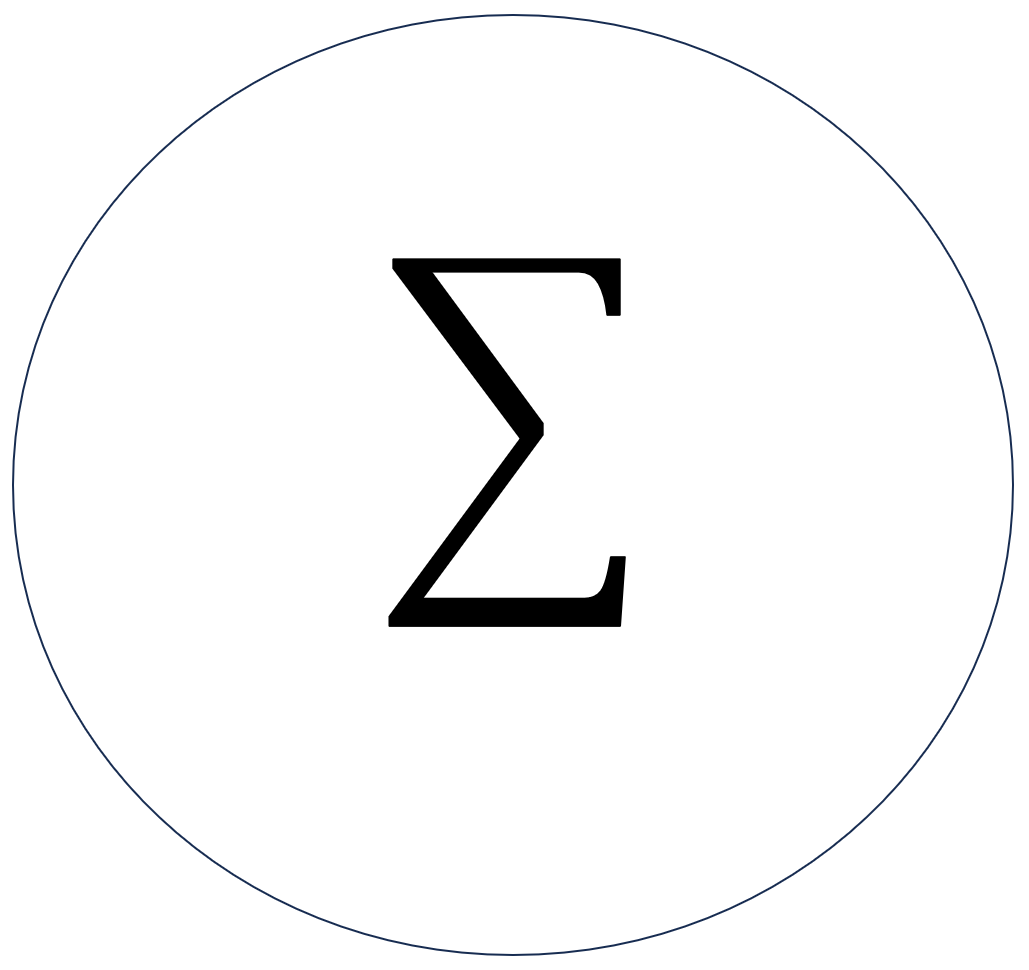
\includegraphics[scale=0.5]{img/QuuNote/icon.png}
    \end{figure}
    
    \vspace{\stretch{1}}
    \centerline{\textbf{概要}}
    \noindent
    微分積分学入門についてのノート。\\
    主に、一変数の極限、一変数の微分・積分、実数の無限級数について扱う。
    
    \clearpage
     
    \clearpage
    \part*{このノートを読む前に}
        このノートははじめて微分積分を学ぶ人のためにつくられている。人によってこれまで勉強した数学が違うだろうから、最低限中学校の知識があれば読めるように配慮した。
        ただ、すでに三角関数をはじめとする前提知識を学んだ人もいるだろうから、そういう人はそこの部分を飛ばして読んでも構わない。このノートでは、厳密さと実際の計算への応用の両立を
        目指し、二年生の微分積分学Iが丸暗記の勉強にならず、円滑に授業を受けられるようにしたつもりである。しかし、中途半端に厳密で不満に思う人もいるかもしれない。そんな人のために
        ノートの最後に参考書籍を上げている。ぜひ参考にしてほしい。

        演習問題についてだが、それぞれの話題で最低限抑えておくべき問題を中心に選んだつもりである。それに加えて、内容に関連する面白い問題等も加えている。そうなると必然的に、学んだあといきなり解くには難易度が
        高すぎるもの含まれてしまう。問題が解けなくても落ち込む必要はないのである。むしろ、5分考えてわからない問題はさっさと解答を見たほうが何倍も自分の勉強になると思う。ただし、最初から答えを見るのは論外である。

        本来なら、微分積分の発明の歴史も詳しく述べられたらよかったが、書く気力がなかったので書かなかった。気になる人は各自で調べてほしい。

        このノート中では同じ表式でも別の記号使っていることがある。例えば、$\sin^{-1}$と書いたり$\arcsin$と書いたり。本来ならどちらかに統一すべきだが、ここではどちらの記法にも慣れてもらうために
        意図的に混同して使っている。しかし、これに限らずだが、意図しない間違い等もあるかもしれない。その時は遠慮せず報告をお願いしたい。

        これを一度読んですべてを理解できる人はまずいないだろうし、その必要もない。わからないところは何回も読んで\footnote{ちなみに、どこかの解析の本では声に出して読むとよいと書いてあった。}、考えることが大切だ。

        このノートの最後でも述べているが、ここに書かれている内容は今後の数学の基礎となる非常に重要なものである。このノートの内容をある程度身に着けたら、今度はもっと高度な内容に挑戦してほしい。
        いきなり難しい本に挑戦するのもよいし、簡単な本から順番に読んでいくのもよいと思う。
        
        これを読んで少しでも微分積分が面白いと思ってもらえたら幸いである。$\square$\\

        以下このノートを書く際に使ったアプリケーション等をあげておく。
        \begin{enumerate}
            \item \TeX (正確には\LaTeX)
            \item VSCode(テキストエディタ)
            \item PowerPoint(主に図を作成するときに用いた)
            \item \href{https://www.wolframalpha.com/}{WolflamAlpha}(検算で大活躍した)
            \item \href{https://www.geogebra.org/graphing}{GeoGebra 関数グラフ}(主に関数を描画する際に用いた)
        \end{enumerate}

        


        
    \clearpage
    \label{目次}
    \tableofcontents
    \clearpage
    
    \part{前提知識}
    \vspace{\stretch{1}}
    \begin{screen}
        微分積分を学ぶうえで前提となる知識をまとめた。微分積分は主に関数の微分・積分について扱うわけだから、ある程度の関数の扱い方も知っておく必要がある。
        そのほか数の種類についてや閉区間・開区間、極限についてもまとめてある。極限は微分積分を学ぶ際にいたるところに出てきて、陰から支える縁の下の力持ち的な役割を持つ。極限は一見すると
        代入と同じように見えるが、実は違う。極限は代入だと都合が悪い時にありがたみが実感できる。極限に関連して、無限という概念も登場する。
    \end{screen}
    \clearpage
    \section{様々な`数'と数直線}

        \subsection{数の種類}
            数学を勉強するうえで、様々な数が登場する。まず一番初めに思いつくのが$1,2,3...$といった\textbf{自然数}である。
            次の自然数に$0$と負の符号をつけたものを加えた\textbf{整数}が考えられる。整数同士で足し算、引き算、掛け算を行っても
            その値は整数である。このことを\textbf{和、差、積について閉じている}という。これは$a,b\in \mathbb{Z}$となる任意の$a,b$
            について
            \begin{equation}
                a+b , a-b , a\times b \in \mathbb{Z}
            \end{equation}
            が成り立つことを意味している。

            一方割り算は整数の中に閉じていない。\footnote{例えば$1\div 2$など。}しかし、$0.5,3.14$などの\textbf{有理数}まで数を拡張すれば、その中に商は閉じている。
            つまり、$a,b \in \mathbb{Q}$となる任意の$a,b$について
            \begin{equation}
                \frac{a}{b} \in \mathbb{Q}
            \end{equation}
            となる。よって、数を有理数まで拡張すれば\textbf{四則について閉じている}ことがわかる。

            さらに数の拡張を考えよう。たとえば$x^2-2=0$を満たす$x$について考えてみるには、数を\textbf{無理数}まで拡張しなければならない。
            一般の二次方程式の解も
            \begin{equation}
                x = \frac{-b\pm \sqrt{b^2-4ac}}{2a}
            \end{equation}
            と有理数だけでは表現できないことがわかる。無理数には$\pi,e\footnote{自然対数の底またはネイピア数と呼ばれる。具体的な値は$e=2.71...$}$などの\textbf{超越数}もふくむ。

            私たちの生活の中では有理数と無理数をあわせた\textbf{実数}があれば十分事足りるが、数学の世界ではそうもいかない。先ほどの二次方程式についてより深く調べてみると、
            解を持たない条件(根号の中身が負)があることがすぐに分かる。例えば、$x^2+1 = 0$は$x^2 = -1$と変形できるが、二乗して負になるような数は実数のうちには存在しない。
            よってこの方程式は\textbf{解なし}となる。がしかし、ここで
            \begin{equation}
                i = \sqrt{-1}
            \end{equation}
            となる`数'を定義してあげると、方程式は$x=\pm i$となり、$(実数)+i$を含めた範囲に解をもつことがわかる。
            この数は、今までの実数とは異なる数であり、実数との和,差は直接計算できない。一般に実数$a,b$と$i$を用いて
            \begin{equation}
                z = a + bi
            \end{equation}
            として表した$z$を\textbf{複素数}といい、$i$を虚数単位という。さらに$a$を$z$の実部、$b$を$z$の虚部といい、それぞれ
            $a=\Re z,b=\Im z$と表す。

            先ほど、二次方程式の解を有理数だけでは表現できないといったが、実は無理数を含めてもできない。この複素数を含めることで初めてすべて表現できるようになるのだ。\footnote{もちろんこれで数の拡張が終わるわけではない。しかし微分積分を学ぶうち間は複素数まで拡張すれば事足りる。}
        \subsection{数直線}
            では、数の大小関係をわかりやすくするためにはどうすればよいだろうか。視覚的にわかりやすくするためには数直線を用いればよい。
            \begin{figure}[h]
                \centering
                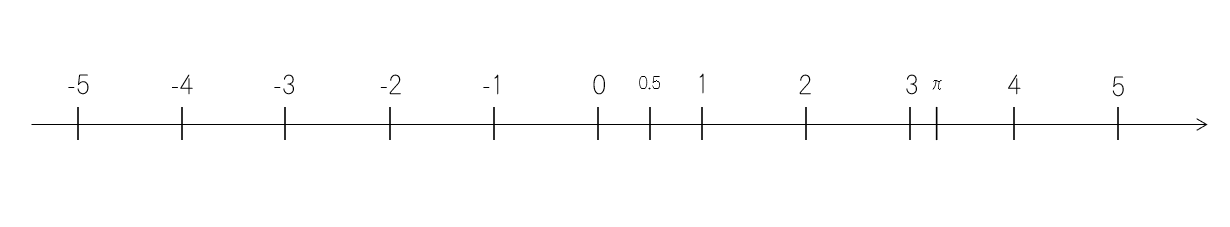
\includegraphics[keepaspectratio,scale=0.5]{img/QuuNote/NumLine_1.png}
                \caption{数直線}
            \end{figure}
            
            上の例では、整数、有理数、無理数の一部を記載している。当然書いてある数以外も数直線の中には含まれている。
            むしろ、数の点の集まりとして数直線を捉える方がイメージがわきやすいかもしれない。
            ここで注意しなければならないのは、この数直線上に複素数$(\Im z\neq 0)$は含まれないといけないということである。
            数直線は\underline{実数を表す}直線なので、複素数のすべては含むことができないのである。

            では実数も含めた複素数はどう表せばよいのか。答えは単純で実数の軸\footnote{これを実軸と呼ぶ。}とは別の軸\footnote{虚軸という。}を
            加えればよい。つまり複素数は平`面'上で表せられるのである。\footnote{この平面を複素平面という。いつものy-xグラフとは見た目は同じだが感覚が違うので注意。}  
            \newpage
        \subsection{開区間・閉区間}
            実数が数直線上の一点で表せることはすでに前項で述べた。では点に続いて次は区間について考えていこう。

            区間は大きく二つある。それらはそれぞれ\textbf{開区間}、\textbf{閉区間}と呼ばれる。これらの違いは端点を含むかどうかで、
            逆に言えば端以外は同じである。例えば、$1<x<2,1\leq x\leq2$について前者は端点$x=1,2$を含まず、後者は端点を含むのである。
            端点を含まない場合が開区間、端点を含む場合が閉区間である。

            閉区間、開区間を数直線上で表すにはどうすればよいだろうか。これも数直線と同様に区間の端から端まで線を引けばよい。注意しないといけないのが
            端点で、区間が開区間か閉区間かによって端点を書き分けないといけない。開区間のときは$\circ$、閉区間のときは$\bullet$と書けばよい。

            \begin{figure}[h]
                \centering
                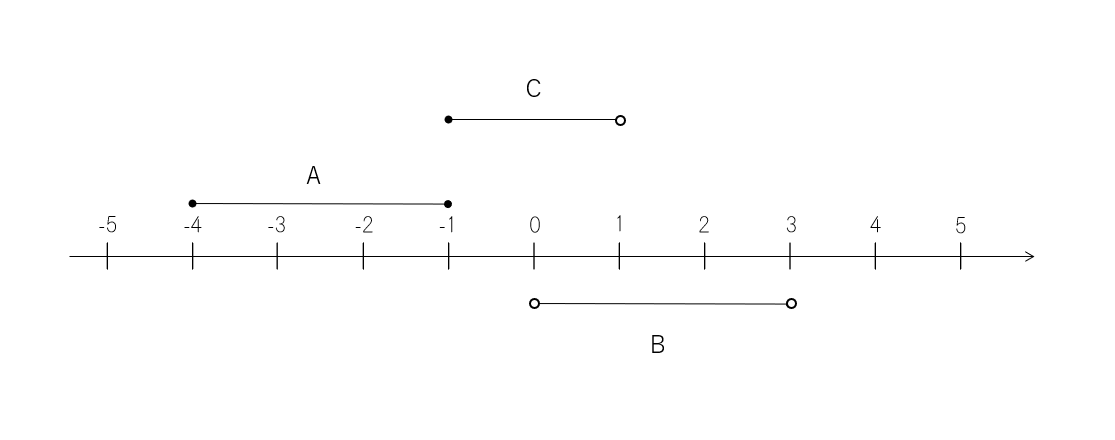
\includegraphics[keepaspectratio,scale=0.7]{img/QuuNote/IntervalLine.png}
                \caption{開区間と閉区間}
            \end{figure}
            例えば上図の例をみてみると、$A,B,C$の三つの区間がある。それぞれ$-4\leq x\leq -1,0<x<3,-1\leq x<1$となる。
            今までは不等号を用いて区間を表現してきたが\footnote{厳密に言えば区間は集合なので、不等号を用いて区間を表現するという言い方は適切ではない。}、もっと簡潔に$(\hspace{1mm}),[\hspace{1mm}]$を用いて表現する方法もある。
            この表現方法を使えば、$A,B,C$はそれぞれ$[-4,-1],(0,3),[-1,1)$と表せる。$(\hspace{1mm})$が等号を含まない、$[\hspace{1mm}]$が
            等号を含む、というわけである。

            では、値が無限に続く(例えば実数全体など)場合はどう表現すればよいのか。この場合は無限大の記号$\infty$を用いて$(-\infty,\infty)$などと表せばよい。\footnote{この方法を使えば、a以上の実数などの場合でも$[a,\infty)$と表せばよいことがわかる。}
            \clearpage
            
        \basicquestion 以下問に答えよ。

        \paragraph{問1}以下の主張のうち正しいものには〇を、間違っているものには×をつけよ。
            \begin{enumerate}
                \item $\sqrt{9}$は無理数である。
                \item 有理数は全て分子分母が整数である分数の形で表せる。
                \item $i$は複素数である。
                \item 有理数の集合は$\mathbb{Q}$として表し、無理数の集合は$\mathbb{N}$で表す。
                \item 自然数全体の集合(区間)は$(0,\infty]$である。
            \end{enumerate}
        \paragraph{問2}以下の区間について、数直線上に示せ。もし数直線上に記されていない数字が出てくる場合はそれも記載せよ。
            \begin{figure}[h]
                \centering
                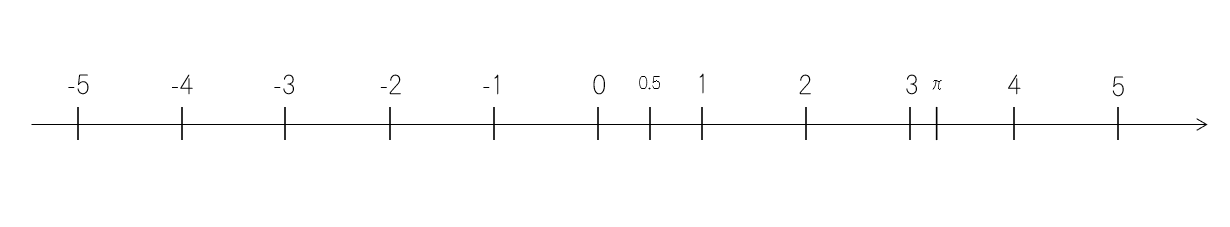
\includegraphics[keepaspectratio,scale=0.6]{img/QuuNote/NumLine_1.png}
                \caption{数直線}
            \end{figure}

            $1.\quad [2,3]$\hspace{3mm}
            $2.\quad (3,5)$\hspace{3mm}
            $3.\quad [-5,\pi]$\hspace{3mm}
            $4.\quad (-2,0.5]$\hspace{3mm}
            $5.\quad [-1,0)$\hspace{3mm}
            $6.\quad (-\infty,0)$\hspace{3mm}
            $7.\quad [0,\infty)$\hspace{3mm}
        \clearpage
        
        \section{関数の性質}
            \subsection{偶関数・奇関数}
                一般の関数$f(x)$について、$f(-x)=f(x)$を満たすものを\textbf{偶関数}、$f(-x)=-f(x)$を満たすものを\textbf{奇関数}という。
                もちろん全ての関数が偶関数・奇関数のどちらかであるというわけではない。しかし、全ての関数は偶関数と奇関数の和で表せられること
                が知られている。\\

                関数が偶関数・奇関数である場合のグラフはどうなるだろうか。まずは偶関数から考えてみると、定義より$x>0$と$x<0$の点において$f$は
                同じ値を取るわけであるから、グラフはy軸に対して対象になるはずである。つぎに奇関数について考えてみよう。これも定義より$x>0$と$x<0$の
                点において、$f$はx軸に対してそれぞれ対象に点を取るはずである。つまり、グラフは原点に対して点対象になるはずである。\\

                偶関数の例となる関数は、$x^2,\cos x,a(\text{定数関数})$などがあげられる。奇関数の例となる関数は、$x,\sin x,\tan x$などがあげられる。
                各自でグラフソフトなどでグラフを見てみるとよい。
            \clearpage
            \subsection{べき関数}
                関数のなかでもっともなじみやすいのが、$f(x)=x^n$であろう。例えば$x$は一次関数、$x^2$は二次関数と呼ばれる。
                別に$n$は自然数に限らなくてもよい。$x^{\frac{1}{2}}=\sqrt{x}$は指数が自然数ではないが、これもべき関数の一つである。
                $n$が自然数のうちは、関数の定義域について特別意識をする必要はない。しかし$n=\frac{1}{2}$などのように指数が有理数であったり、
                $n=-1$のように指数が負の値を取る場合には定義域に十分注意する必要がある。このように、一般に$f(x)=x^n$で表される関数を\textbf{べき関数}という。

                次に関数のグラフについて、グラフ描画ソフトを用いて数式を入力すると以下のようになる。
                \begin{figure}[h]
                    \centering
                    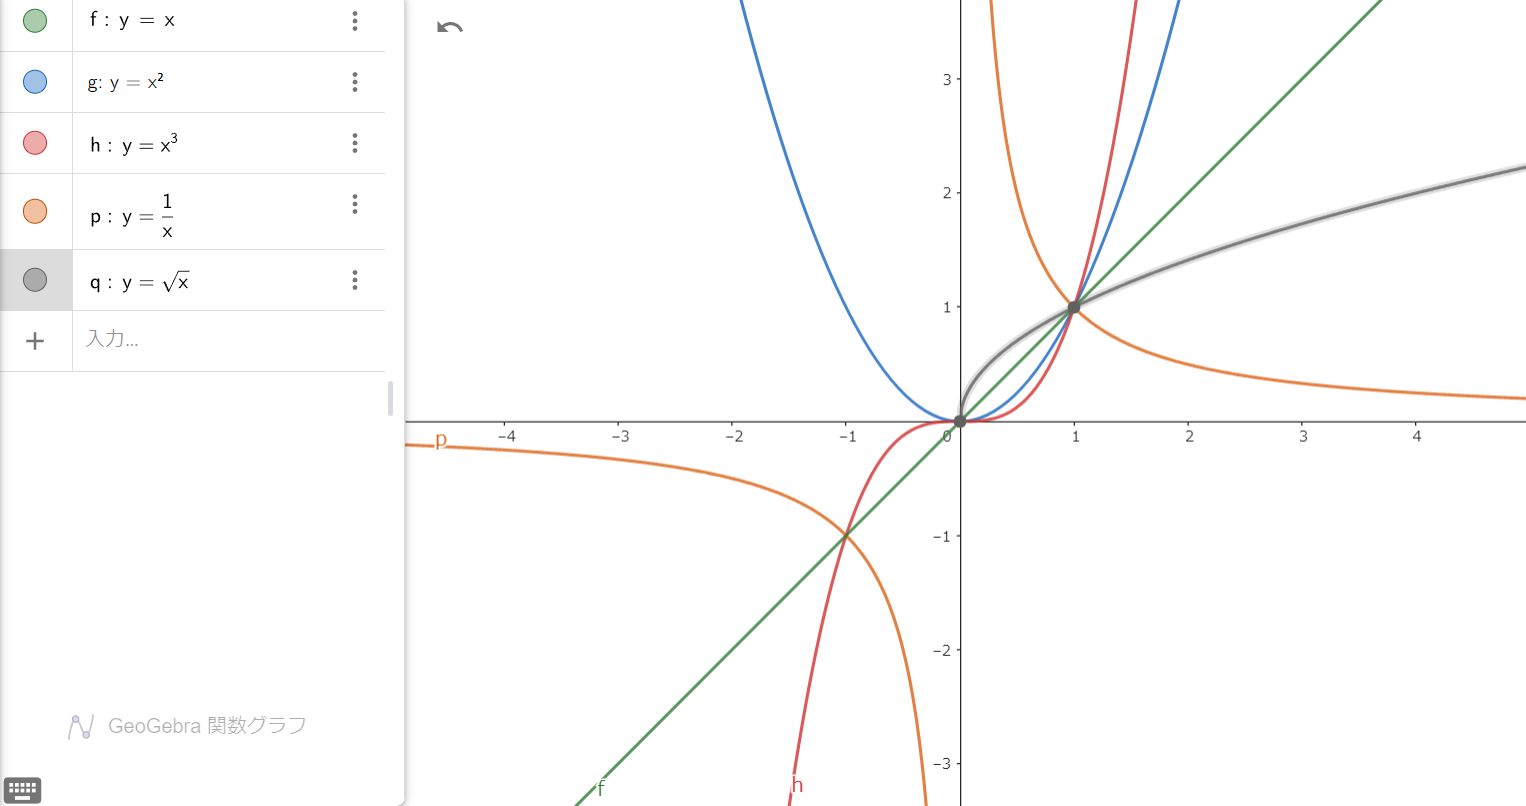
\includegraphics[keepaspectratio,scale=0.5]{img/QuuNote/PowerFuncGraph.png}
                    \caption{べき関数グラフ}
                \end{figure}

                図からも$\sqrt{x}$が$x<0$で定義されないことがわかる。また、$x^2$と$\sqrt{x}$は$y=x$を軸にして線対象になっており、
                $x^2$と$\sqrt{x}$は互いに\textbf{逆関数}であることがわかる。
            \clearpage
            \subsection{三角関数}
                \textbf{三角関数}は三角比を一般角に拡張した関数である。直交座標から極座標に変換する際などにしばし用いられる。
                三角比の定義自体を忘れた人はいないだろうが一応説明しておく。
                \begin{figure}[h]
                    \centering
                    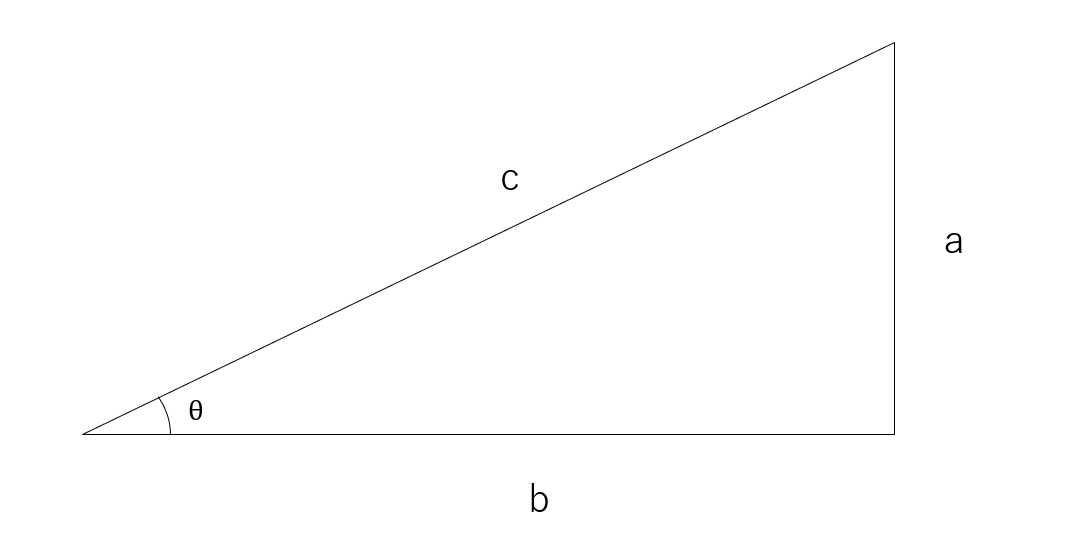
\includegraphics[keepaspectratio,scale=0.3]{img/QuuNote/triangleFunc.png}
                    \caption{三角比}
                \end{figure}

                上図\footnote{aの辺のことを対辺、bの辺のことを隣辺、cの辺のことを斜辺という。}において
                \begin{align}
                    \sin \theta &= \frac{a}{c}\\
                    \cos \theta &= \frac{b}{c}\\
                    \tan \theta &= \frac{a}{b}
                \end{align}
                また、定義より$\displaystyle\tan \theta = \frac{\sin \theta}{\cos \theta}$が成り立つ。

                三角関数には様々な公式がある。\footnote{公式集を眺めるとやたらと二乗がついていることがわかる。つまり三角関数は\underline{二乗に強い}のである。この性質は積分を解く際に重要である。}
                しかしそれらは単位円を書けばすぐに導けるので、一部を除いて割愛する。
                また、二倍角の公式などについても、全て\textbf{加法定理}より導けるのでここでは加法定理のみ紹介する。

                \begin{align}
                    \sin^2 x + \cos ^2 x &= 1 &\quad 1 + \tan^2 x &= \frac{1}{\cos^2 x}\\
                    \sin\left(\frac{\pi}{2}-x\right) &= \cos x &\quad \cos\left(\frac{\pi}{2}-x\right) &= \sin x\\
                    \tan\left(\frac{\pi}{2}-x\right) &= \frac{1}{\tan x} &&
                \end{align}
                \begin{align}
                    \sin(\alpha\pm\beta) &= \sin\alpha\cos\beta \pm \cos\alpha\sin\beta\\
                    \cos(\alpha\pm\beta) &= \cos\alpha\cos\beta \mp \sin\alpha\sin\beta\\
                    \tan(\alpha\pm\beta) &= \frac{\tan\alpha\pm\tan\beta}{1\mp\tan\alpha\tan\beta}
                \end{align}
                また、三角関数は\textbf{周期関数}である。$\sin x,\cos x$は周期$2\pi$、$\tan x$は周期$\pi$である。
            \clearpage
            \subsection{指数・対数関数}
                `指数関数的に増加する'という言葉をよく耳にする。これは、なにか爆発的な増加の様子を示している表現である。このように、\textbf{指数関数}は$x$の値が少し変わるだけで値が
                大きく増加・減少する関数である。その具体的な表式は$a^x$と表される。指数の部分が変数になっているのである。

                指数関数は、$a$の値によって性質が少し異なる。$0<a<1$の場合には単調減少関数となり、$1<a$の場合には単調増加関数になる。
                このとき$a$が負の値の場合は定義しない。\footnote{例として$(-2)^x$のグラフを書いてその理由を考えてみるといい。}\footnote{実際は定義することができるがその際には複素関数の知識が必要。なので今回は扱わない。}

                以下、指数法則について述べる。$a,b>0\quad x,y\in \mathbb{R}$とすると、
                \begin{align}
                    a^x\cdot a^y&=a^{x+y}\\
                    \frac{a^x}{a^y} &= a^{x-y}\\
                    (a^x)^y &= a^{xy}\\
                    (ab)^{x} &= a^x\cdot b^x
                \end{align}

                指数関数のグラフは、以下のようになる。
                \begin{figure}[h]
                    \centering
                    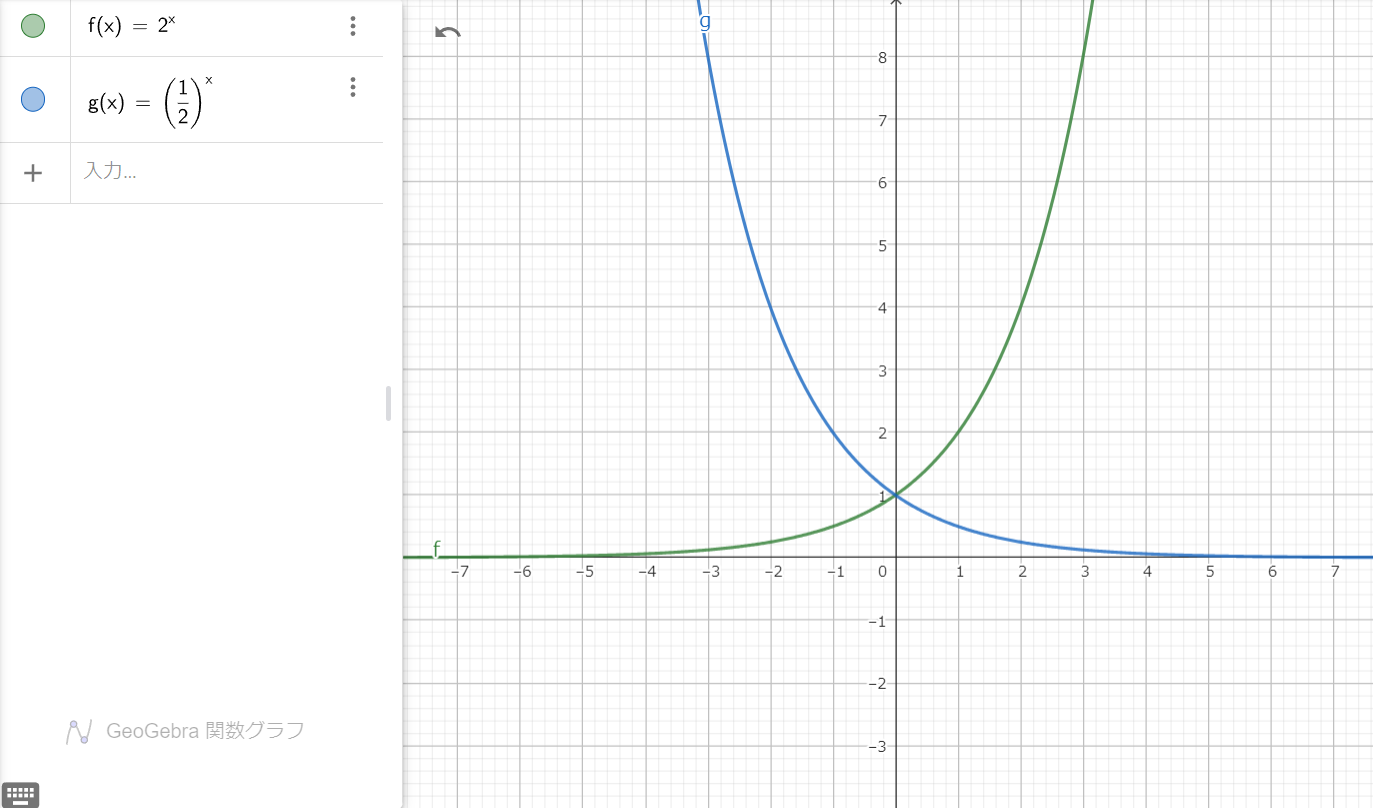
\includegraphics[keepaspectratio,scale=0.3]{img/QuuNote/ExpFuncGraph.png}
                    \caption{指数関数のグラフ}
                \end{figure}

                グラフから、$a$が1より大きくても小さくても$x=0$で$y=1$を取ることがわかる。

                なお、底が$e$の場合の指数関数は$e^x=\exp{x}$と書くこともある。\\

                では次に、指数関数の逆関数を考えてみよう。指数関数の逆関数は与えられた値に対して、
                底を何回掛けたらその値になるかの回数を表す関数である。つまり、指数関数の底ごとに
                逆関数が存在する。文章で見てもわかりずらいので数式で以下示す。

                \begin{equation}
                    f(x)=a^x \leftrightarrow x = f^{-1}(y) = \log_a{y}
                \end{equation}
                指数関数の逆関数は底が何かを示さないといけないので、逆関数$\log$に下付き文字で書く。
                しかし、底が$e$だった場合は省略して$\log y$と書いてもよい。この関数を\textbf{自然対数}という。\footnote{自然対数は$\ln x$と書くこともある。natural logarithmのことである。}
                底が$e$じゃない場合は単に対数と呼ぶ。\footnote{底が10の場合は常用対数という。}

                以下、対数の性質を述べる。必要ない限り底は省略して記載する。指数法則と見比べると理解が深まる。

                \begin{align}
                    \log(xy)&=\log x+\log y\\
                    \log\left(\frac{x}{y}\right)&=\log x - \log y\\
                    \log(a^b) &= b\log a \\
                    \frac{\log_c b}{\log_c a}&=\log_a b\qquad(\text{\textbf{底の変換公式}})
                \end{align}

                また、対数の定義より
                \begin{equation}
                    \log 1 = 0\quad \log_a a = 1
                \end{equation}
                が成り立つ。対数関数$\log x$の引数$x$のことを真数と呼び、これは$x>0$である。\footnote{真数が正であるという条件のことを真数条件という。}

                対数関数のグラフは以下のようになる。

                \begin{figure}[h]
                    \centering
                    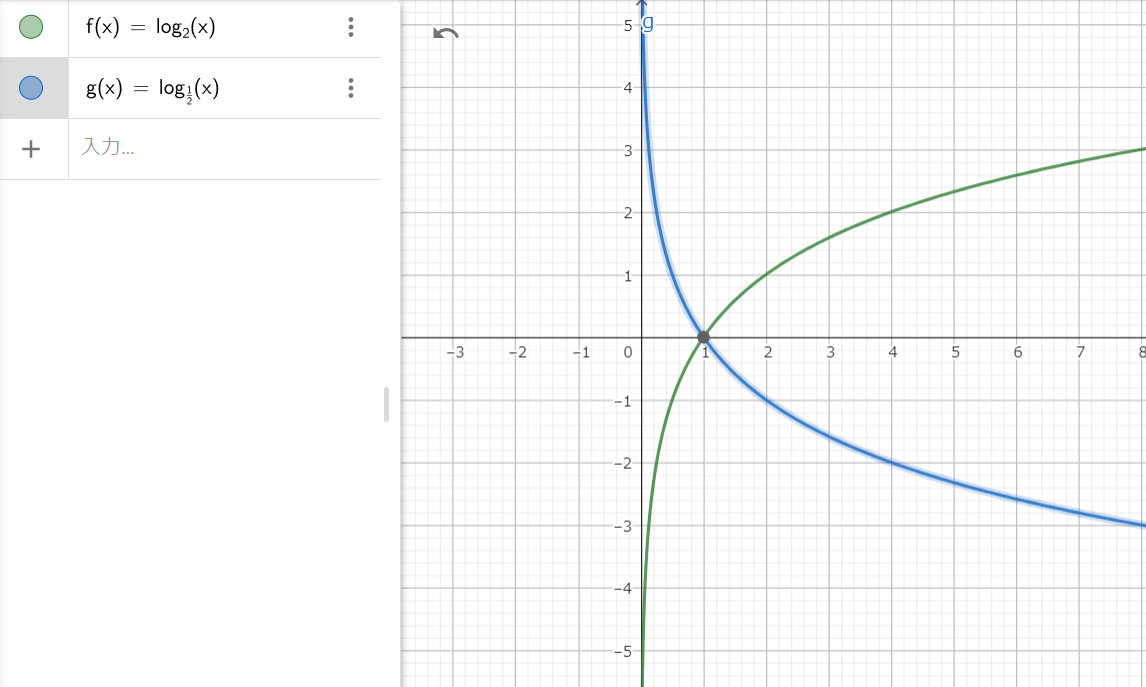
\includegraphics[keepaspectratio,scale=0.5]{img/QuuNote/LogFuncGraph.png}
                    \caption{対数関数}
                \end{figure}
                
                グラフを見ればわかるように、底が1より大きいか小さいかで単調増加・減少かが変わる。

                対数関数は爆発的に増加・減少する指数関数とは対照的に、値の変化が($x<1$を除いて)緩やかである。
                そのため、値がとても大きい値でも対数を取ることで値のスケールを小さくすることができる。
                また、対数を取ることで\underline{掛け算を足し算にできる}。この性質は非常に重要である。
            \clearpage
            \subsection{逆三角関数}
                指数関数の逆関数である対数関数を考えたのと同じように、三角関数の逆関数も考えてみよう。
                三角関数は与えられた角度に対応するそれぞれの三角比を返す関数である。では三角関数の逆関数は
                与えられた三角比に対応する`角度'を返す関数であることがすぐに分かる。これらを次のように書くことにする。
                \begin{align}
                    \arcsin x &= \sin^{-1} x \\
                    \arccos x &= \cos^{-1} x \\
                    \arctan x &= \tan^{-1} x
                \end{align}
                左辺にちなんで左からそれぞれ「アークサイン」,「アークコサイン」,「アークタンジェント」と読む。これらをまとめて
                \textbf{逆三角関数}という。表記に左辺を用いるか右辺を用いるかは個人の好みによる。\footnote{だからといって、$\frac{1}{\sin x}$を$\sin^{-1}x$と書くことはまずない。}

                三角関数が周期関数であるため、逆三角関数は多価関数であることは容易に想像できる。
                逆三角関数を一価関数にするため、値域をそれぞれ$[-\frac{\pi}{2},\frac{\pi}{2}],[0,\pi],(-\frac{\pi}{2},\frac{\pi}{2})$
                に制限して用いることがある。このことを\ruby{主枝}{しゅし}を取るという。またこの制限した値域を主枝という。
                主枝以外の値域を分枝と呼ぶ。

                逆三角関数が主枝を取っていることを明示するために
                \begin{align}
                    {\rm Arcsin} x &= {\rm Sin^{-1}} x \\
                    {\rm Arccos} x &= {\rm Cos^{-1}} x \\
                    {\rm Arctan} x &= {\rm Tan^{-1}} x
                \end{align}
                のように、先頭を大文字で書くこともある。しかし今回はこの記法は採用しない。

                逆三角関数のグラフは以下のようになる。
                \begin{figure}[h]
                    \begin{minipage}{5cm}
                        \centering
                        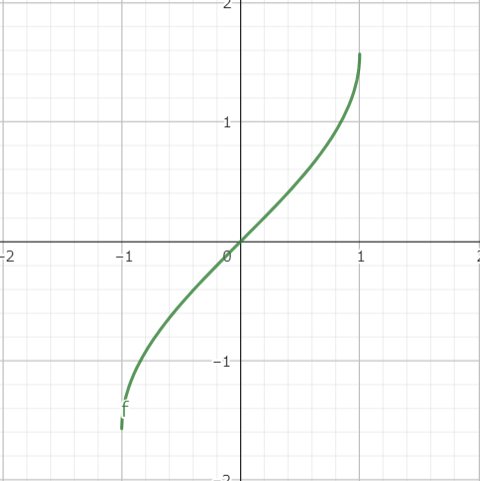
\includegraphics[keepaspectratio,scale=0.3]{img/QuuNote/ArcsinFuncGraph.png}
                        \caption{$\arcsin x$のグラフ}
                    \end{minipage}
                    \begin{minipage}{5cm}
                        \centering
                        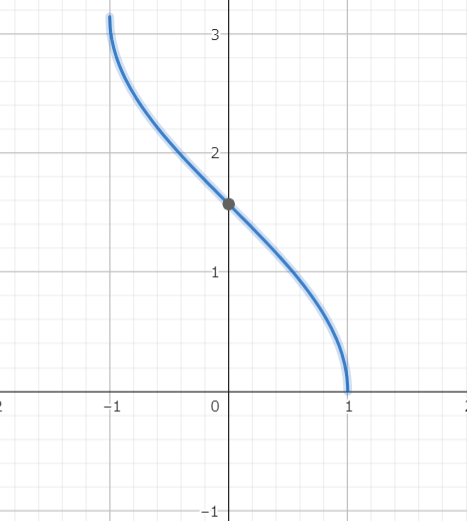
\includegraphics[keepaspectratio,scale=0.3]{img/QuuNote/ArccosFuncGraph_ver2.png}
                        \caption{$\arccos x$のグラフ}
                    \end{minipage}
                    \begin{minipage}{5cm}
                        \centering
                        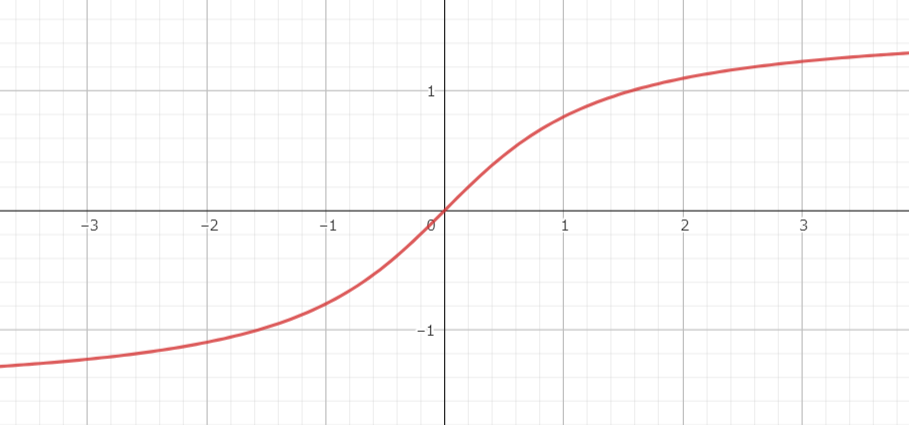
\includegraphics[keepaspectratio,scale=0.3]{img/QuuNote/ArctanFuncGraph.png}
                        \caption{$\arctan x$のグラフ}
                    \end{minipage}
                \end{figure}
                
                もちろん主枝を取らない場合は、それぞれと同じグラフが上や下につながっていく。\\

                三角関数の公式から、逆三角関数についても公式が導ける。例えば、
                \begin{equation}
                    \sin^{-1} x+\cos^{-1} x =\frac{\pi}{2}
                \end{equation}
                ほかにも公式が導けるので、各自で考えてみるとよい。
            \clearpage
            \subsection{双曲線関数}
                いきなりだが、次のように関数を定義する。$e$はネイピア数である。
                \begin{align}
                    \sinh x &= \frac{e^x - e^{-x}}{2}\\
                    \cosh x &= \frac{e^x + e^{-x}}{2}\\
                    \tanh x &= \frac{\sinh x}{\cosh x} = \frac{e^x - e^{-x}}{e^x + e^{-x}}
                \end{align}
                これらは\textbf{双曲線関数}と呼ばれる。読み方はそれぞれ「ハイパボリックサイン」、「ハイパボリックコサイン」、
                「ハイパボリックタンジェント」である。ただこれだと長ったらしいので「シンチ」、「コッシュ」、「タンチ」と呼ぶ
                場合もある。

                見た目が三角関数と酷使しているが、実は性質も似たものを持つ。例えば、$\cosh^2 x - \sinh^2 x = 1$など。
                また、加法定理も符号は若干異なるがほとんど同じ形をしている。

                さらに、オイラーの公式$e^{ix}=\cos x + i\sin x$\footnote{この公式自体はだいぶ後になって解説する。}を用いれば、
                $\sin ix = i\sinh x,\cos ix=\cosh x$が導ける。\footnote{むしろこの性質が成り立つように双曲線関数を定義するといったほうが正しいかもしれない。}\\

                双曲線関数のグラフは以下のようになる。
                \begin{figure}[h]
                    \begin{minipage}{5cm}
                        \centering
                        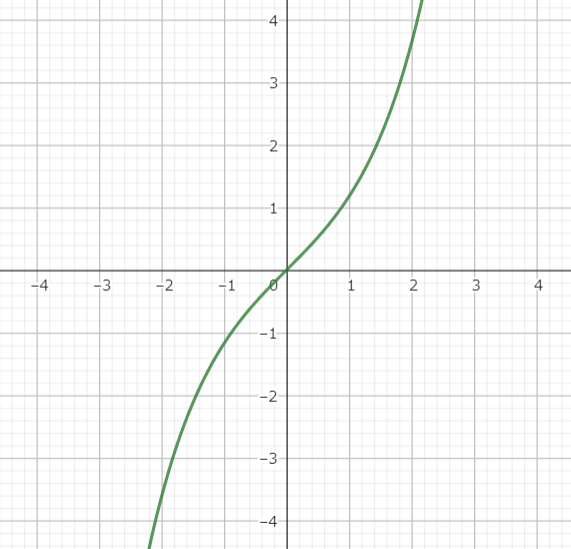
\includegraphics[keepaspectratio,scale=0.3]{img/QuuNote/SinhFuncGraph.png}
                        \caption{$\sinh x$のグラフ}
                    \end{minipage}
                    \begin{minipage}{5cm}
                        \centering
                        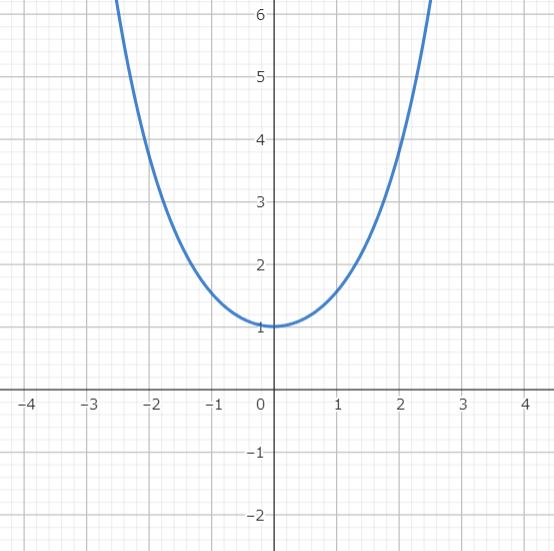
\includegraphics[keepaspectratio,scale=0.3]{img/QuuNote/CoshFuncGraph.png}
                        \caption{$\cosh x$のグラフ}
                    \end{minipage}
                    \begin{minipage}{5cm}
                        \centering
                        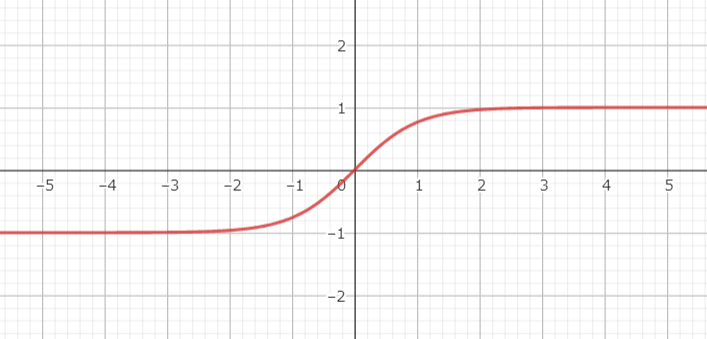
\includegraphics[keepaspectratio,scale=0.3]{img/QuuNote/TanhFuncGraph.png}
                        \caption{$\tanh x$のグラフ}
                    \end{minipage}
                \end{figure}

                $\cosh x$のグラフはカテナリーと呼ばれる。電柱などの垂れた線はこれにあたる。
            \clearpage
            \subsection{初等関数}
                前節まで述べたべき関数、三角関数、指数・対数関数、逆三角関数は\textbf{初等関数}という。
                また、それらの関数からなる多項式の関数や初等関数の合成関数は初等関数である。例えば、双曲線関数は
                $e^x,e^{-x}$の和でなっているが、これらは初等関数なので双曲線関数も初等関数である。

                しかし初等関数の逆関数は必ずしも初等関数であるとは言えない。よく例に挙げられるのが$f(x)=xe^x$の逆関数である。
                この関数はランベルトのW関数とよばれ、$f^{-1}(x)=W(x)$と書かれる。

                初等関数は性質がよく知られているので、微分・積分するうえで比較的扱いやすい。初等関数を微分したもの
                も初等関数であるが、初等関数を積分したものが必ずしも初等関数である保証はない。とはいえ今は微分も積分も知らないわけだから、
                単に事実として受け入れるだけでよい。\\

                初等関数に対して高等関数というものもある。これは初等関数以外の関数のことで、初等関数よりも数は多い。
                先ほど紹介したランベルトのW関数以外には以下のようなものがある。

                \begin{align}
                    \Gamma(s) &= \int_0^\infty e^{-x}x^{s-1}dx\qquad&&(\text{\textbf{ガンマ関数}})\\ 
                    B(p,q) &= \int_{0}^{1} x^{p-1}(1-x)^{q-1}dx\qquad&&(\text{\textbf{ベータ関数}})\\
                    {\rm Li}(x) &= \int \frac{dx}{\log x}\qquad&&(\text{\textbf{対数積分}})\\
                    \zeta(s) &=  \sum_{n=1}^{\infty}\frac{1}{n^s}\qquad&&(\text{\textbf{ゼータ関数}})
                \end{align}

                もちろんこれ以外にも様々な関数がある。興味があったら調べてみるといい。
                \clearpage
                \basicquestion 以下の問いに答えよ。

                \paragraph{問1}次の関数が偶関数か奇関数かを判別せよ。

                \noindent
                (1)$x\sin x$\hspace{3mm}
                (2)$x^5$\hspace{3mm}
                (3)$\sinh x$\hspace{3mm}
                (4)$\log|x^2|$\hspace{3mm}
                (5)$x^3+x+\sin x$\hspace{3mm}
                (6)$e^{-x}$\hspace{3mm}
                (7)$f(\cos x)$\hspace{3mm}
                (8)$\arctan x$

                \paragraph{問2}以下の等式を証明せよ。

                \noindent
                $(1)\sin 2x=2\sin x\cos x/\cos 2x=\cos^2 x-\sin^2 x$(\textbf{倍角の公式})\\
                $(2)\displaystyle \sin^2\frac{x}{2}=\frac{1-\cos x}{2}/\cos^2\frac{x}{2}=\frac{1+\cos x}{2}$(\textbf{半角の公式})\\
                $(3)\sinh(x+y)=\sinh x\cosh y + \cosh x\sinh y/\cosh(x+y)=\cosh(x+y)=\cosh x\cosh y + \sinh x\sinh y$\\
                
                \paragraph{問3}以下の値を求めよ。

                \noindent
                $(1)\sin \pi+\cos \frac{3}{2}\pi + \tan(-\pi)$\hspace{3mm}
                $(2)\arcsin(\frac{1}{2})$\hspace{3mm}
                $(3)\arccos(1)$\hspace{3mm}
                $(4)\log_28$\hspace{3mm}
                $(5)\log_a(\tan(\frac{\pi}{4}))\quad(a>1)$\\
                $(6)\log_63+\log_62$\hspace{3mm}
                $(7)\arcsin(1-\log\pi)-\cos(\log2)\sin(\log 3)+\sin(\log3 -\log 2)-\log e^{\arccos(\log \pi-1)}$

                \paragraph{問4}対数を使えば桁数の多い数字同士の掛け算を足し算で計算することができる。簡単な例として$271\times 314$を
                対数を用いて計算せよ。ただし、常用対数$\log_{10} 2.71\simeq0.4346,\log_{10} 3.14\simeq0.4969,10^{4.9315}\simeq85408$は用いてよい。
                
                \paragraph{問5}$t=\tan\frac{x}{2}$とするとき、$\sin x,\cos x,\tan x$をそれぞれ$t$を用いた式で表せ。\footnote{ヒント:半角の公式を用いる。}
            \clearpage
            \section{極限}
            \subsection{数列の極限}
                \textbf{数列}とは、数字をある規則によって並べた列のことで、例えば$1,2,3,4,\cdots,100$などがある。
                この数字に左から順に番号付けすることを考える。そのときある数列$\{a_n\}$について、左から$n$番目の数値を$a_n$
                と表し、第$n$項とよぶ。特に$n=1$の一番初めの項$a_1$を初項という。
                数列には等差数列や階差数列があるがここでは詳しく述べない。

                項の数は有限でも無限でもよいので、項が無限にある数列$\{a_n\}$について考えてみることにする。$n$を限りなく大きくすると
                数列の値がある一定の値$a$に近づくときがある。この時数列$\{a_n\}$は\textbf{収束する}といい、近づく値$a$を\textbf{極限値}
                という。これを数式で表すと
                \begin{equation}
                    \lim_{n\to \infty}a_n=a
                \end{equation}
                新しく$\lim$という記号が出てきたが、これは$n$を限りなく大きくする(無限大に近づける)という操作を表す記号である。
                $a_n\to a \hspace{1mm}(n\to\infty)$と書いてもよい。このとき$a_n=a$となる$n$が存在する必要はない。
                
                \paragraph*{例}$\{a_n\}=1-\frac{1}{n}$について考える。$n$を限りなく大きくすると$\frac{1}{n}$は限りなく小さくなる($0$に近づく)ので
                $a_n$は$1-0=1$に近づく。よって$\{a_n\}$は収束し、極限値は$1$。\\

                始めのうちは値が近づく、と言われても何をどうすればよいかわからないであろうから、代入のような何かという風にとらえてもよい。実際極限のほとんどの操作は
                代入と結果的に等しくなる。気を付けないといけないは代入だと定義できない$\frac{1}{0}$などの場合である。\\

                極限の性質について以下にまとめる。$\displaystyle\lim_{n\to\infty}a_n=a,\lim_{n\to\infty}b_n=b,cは定数$とする。
                \begin{align}
                    \lim_{n\to\infty}(a_n\pm b_n)&=a\pm b\\
                    \lim_{n\to\infty}(c\cdot a_n)&=c\cdot a\\
                    \lim_{n\to\infty}(a_n\cdot b_n)&=a\cdot b\\
                    \lim_{n\to\infty}\frac{a_n}{b_n}&=\frac{a}{b}\quad(b_n\neq 0,b\neq 0)
                \end{align}

                収束するとは$n$を限りなく大きくしたときに数列が有限の値に近づくことだが、これはより厳密に言うことができる。
                \begin{itembox}{数列の収束の定義}
                    数列$\{a_n\}$が$a$に収束する$\Leftrightarrow $任意の$\varepsilon>0$が与えられたとき、それに対応してある$N$が\fbox{$n>N$のとき$|a-a_n|<\varepsilon$}となるように定められる。
                \end{itembox}
                正直一目見ただけでは全然意味がわからないはず。少しずつ理解していこう。この定義は二つに分けると見やすい。
                まず、任意の$\varepsilon$、つまりどんな$\varepsilon>0$に対しても、(収束するなら)対応する$N$\footnote{限定記号を使えば$\forall \varepsilon>0,\exists N\in\mathbb{N}$となるので、$N=N(\varepsilon)$と書いてもよい。}が必ず見つかるということを言っている。
                ただ、このままだとなにをどう対応する$N$なのかがはっきりしない。そこで四角で囲った条件が必要になる。ざっくり言ってしまえば
                \underbar{正数$\varepsilon$がどんな値でも、四角で囲った条件を満たす$N$が見つかる}ということになる。

                次に四角で囲った条件について詳しく見ていこう。始めの条件$n>N$は一旦無視して、$|a-a_n|<\varepsilon$に注目する。
                この不等式の左辺が何を表すかを考えてみよう。数直線上に$a,a_n$をプロットすると、$|a-a_n|$はそのプロットした点と点
                との距離を表す。つまり不等式は、「近づく(であろう)値と$a_n$との距離をどんなに小さくとっても\footnote{$\varepsilon$は任意の数なのでどんなに小さくとってもよい。
                反対に大きくとることもできるが、$<\varepsilon$なので大きくとることに言及する意味はない。}」という意味になる。
                ここで飛ばした$n>N$についてみてみると、これは$n$が$\varepsilon$によって決まる$N$より大きい、という意味であるから、
                四角の条件をまとめると「近づく(であろう)値と$a_n$との距離をどんなに小さくとっても、その小さくとった幅に対応して$n$を大きくとれる」ということになる。\\

                とはいえ、これを文章で説明されても全然イメージがわかない。ということで実際に値をプロットしてみた。
                \begin{figure}[h]
                    \centering
                    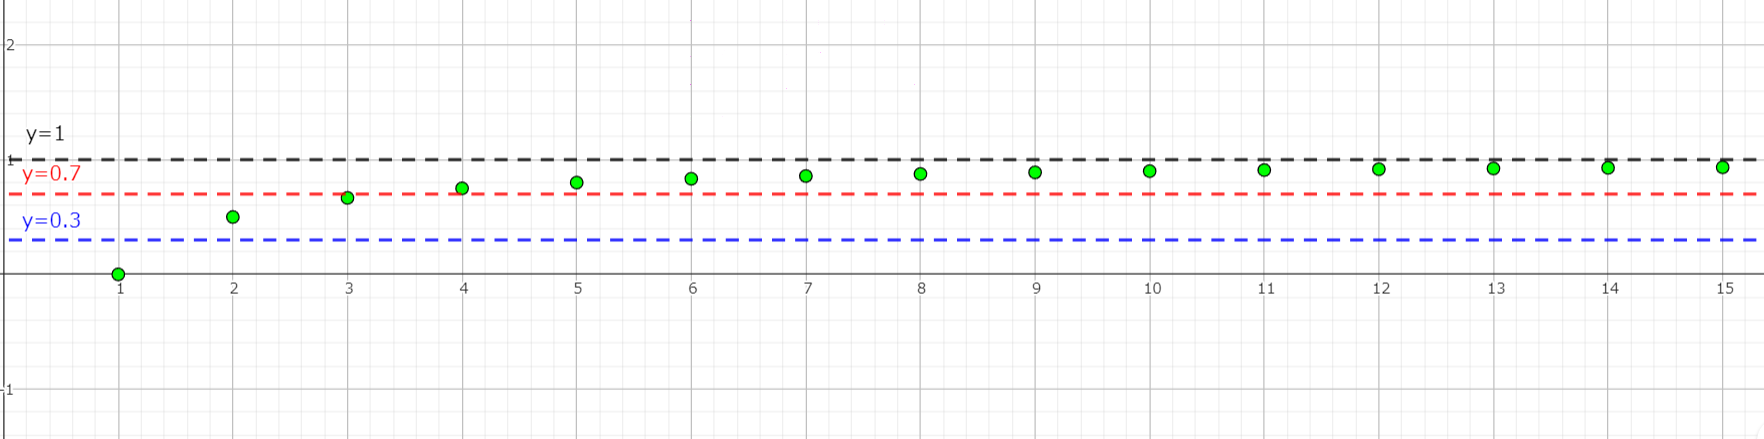
\includegraphics[keepaspectratio,scale=0.45]{img/QuuNote/SequeanceLimitGraph.png}
                    \caption{$\{a_n\}=1-\frac{1}{n}$のグラフ}
                \end{figure}
                
                この数列で「$\varepsilon=0.7$を取るとき、$|a-a_n|=\frac{1}{n}<0.7\to n> 1=N$となるように$N$を取れば、$n>N$となる全ての$a_n$は
                図中の黒線と青線の間に入っている」が成り立っている。
                次の「$\varepsilon=0.3$を取るとき、$|a-a_n|=\frac{1}{n}<0.3\to n>3=N$となるように$N$を取れば、$n>N$となる全ての$a_n$は
                図中の黒線と青線の間に入っている」も成り立っている。

                このように「黒線との距離がどんなに小さな点線を考えても、ある番号$N$以上なら黒線とその小さい点線の間にプロットされる。そのような$N$が必ず見つかる。」というのが収束の定義の主張である。\\

                この収束の定義はとても難しい話なので、理解するのに時間がかかるかもしれない。(丁寧に説明したつもりけど、逆に回りくどくなってわかりにくいかも)そんな時は一旦飛ばすというのも手である。
                もちろんここで立ち止まって考えてもいいが一旦放置してあとから見直すとわかる、なんてこともざらにある。\\

                {\color{blue}$\diamondsuit$収束する数列はすべて有界\footnote{有界とは全ての$n$に対して$m\leq a_n \leq M$である定数$m,M$が存在すること。}である。\footnote{詳しい話は無限級数を扱うときに述べる。}}
            \clearpage
            \subsection{関数の極限}
                次の関数の極限について述べる。数列と違い、無限大以外に近づける場合も出てくる。ひとまず定義域$x\in I=(a,b)$である関数$f(x)$と
                定数$c\in I$を考えよう。$x$の値を$c$に限りなく近づけたとき、$f(x)$の値がある一定の値$C$に近づくとする。
                このとき
                \begin{equation}
                    \lim_{x\to c}f(x)=C
                \end{equation}
                と表し、$f(x)$は\textbf{収束する}という。また、$C$を$x$を$c$に近づけたときの$f(x)$の\textbf{極限値}という。記号の使い方は数列と同じなので馴染みやすい。
                もちろん$f(x)\to C\quad(x\to c)$という書き方もできる。
                
                \paragraph{例}$\displaystyle\lim_{x\to 2}x^2 = 4$ $x<2$の点からでも$x>2$の点からでも$2$に近づければ$f(x)=4$に近づく。これはグラフを見ても直感的にわかる。\\
                
                いま$c$は$f(x)$の定義域に含まれている状態で考えてみるが、実は含まれていなくてもよい。
                例えば、$f(x)=\frac{x^2-1}{x-1}$は$x=1$で定義出来ないが、$x\neq 1$で$f(x)=x+1$であるから$x\to 1$の
                極限を取ると値は$2$に近づく。このような例で極限と代入との違いがはっきりとわかる。\\

                いま近づけている値は有限の値を想定しているが、数列のように無限大(小)に大きくする極限も考えることが考えることができる。
                \begin{equation}
                    \lim_{x\to\infty}f(x)\quad \lim_{x\to-\infty}f(x)
                \end{equation}
                のように書く。例えば、$\displaystyle\lim_{x\to \pm\infty}\frac{1}{x}=0$。
                
                \noindent
                極限の性質の公式は、数列と同様であるためここでは述べない。\\

                さて、数列の極限と同様、関数の極限でもより厳密な定義について考えてみよう。それは以下のようになる。
                \begin{itembox}{関数の極限の定義}
                    $f(x)$が$x\to a$で$b$に収束する$\Leftrightarrow$任意の$\varepsilon>0$が与えられたとき、それに対応してある$\delta > 0$が\fbox{$0<|x-a|<\delta$のとき$|f(x)-b|<\varepsilon$}
                    となるように定められる。
                \end{itembox}
                これはいわゆる\textbf{$\varepsilon-\delta$論法}と呼ばれるもので、ぶっちゃけめっちゃ難しい。ただこれも落ち着いてみれば数列の極限の定義\footnote{$\varepsilon-N$論法という。}と似通っているところがあることに気づける。

                数列の極限との違いは$x$の範囲の制限にある。数列の場合は$x>N$だったが、関数の場合は$|x-a|<\delta$となっている。$N,\delta$の役割は同じなので今はただ記号を変えているだけと考えてよい。
                $|x-a|$は$x$と$a$との数直線上での差、つまり二つの点の距離を表しているので、$|x-a|<\delta$はその距離が$\delta$より小さいときというのを表している。
                あとは数列の場合と大体同じで、どんなに$f$と極限値が近づいていても($\varepsilon$を小さくしても)それに対応する$\delta$の値が定められる($x$が$a$に近づく)ということになる。
                \newpage

                $\varepsilon-\delta$論法を使って、実際に収束することを証明してみる。
                \paragraph*{例}$\displaystyle\lim_{x\to 2}x^2=4$を証明する。\\
                $0<|x-2|<\delta$とするとき、$|x^2-4|=|x-2|\cdot|x+2|=|x-2|\cdot|(x-2)+4|\leq |x-2|^2+4|x-2|<\delta^2+4\delta$
                であるため、$\varepsilon=\delta^2+4\delta\leftrightarrow \delta = -2+\sqrt{4+\varepsilon}$となるように$\delta$を取ればよい。このとき$0<|x-2|<\delta\rightarrow|x^2-4|<\varepsilon$を満たすので証明が終わる。$\square$\\

                試しに、$\varepsilon = 0.1$を代入すると$\delta \thickapprox 0.02484$であるため、$x=2.02483$のとき$|x^2-4|<\varepsilon$を満たすはずである。
                実際、$|x^2-4|=0.0999770256<0.1=\varepsilon$となっていて満たしている。今回は具体的に$\delta(\varepsilon)$を求めたが、このやり方にとらわれなくても四角で囲った条件を満たすように$\delta$が
                取れればよい。\\

                ここまで関数の収束について述べたが、ある一定の値に近づかずそのまま値が無限大に増大する場合などについて考えてみる。
                例えば、$x^3$は$x\to\infty$で$x^3\to\infty$である。このような場合\textbf{無限大に発散する}という。
                もちろん負の無限大に発散する場合も考えられる。一方で、$\sin x$は$x\to\infty$で値が無限大に増大するわけではないが、
                値が一つに定まることもない。このような場合は\textbf{振動する}という。\footnote{$\sin x$のグラフを見れば「振動する」という言い方がぴったりだとわかる。}\\

                次に重要な極限の公式を述べる。
                \begin{align}
                    \lim_{x\to 0}&\frac{\sin x}{x}=1\label{eq:limit of sin/x}\\
                    \lim_{x\to 0}&\left(1+x\right)^\frac{1}{x} = e\label{eq:define_e}
                \end{align}
                式\eqref{eq:define_e}はネイピア数の定義である。実際は左辺の極限が収束することを証明しないといけないが、ここでは割愛する。

                では式\eqref{eq:limit of sin/x}を証明する。
                \paragraph{証明}下図のような単位円を考える。
                \begin{figure}[h]
                    \centering
                    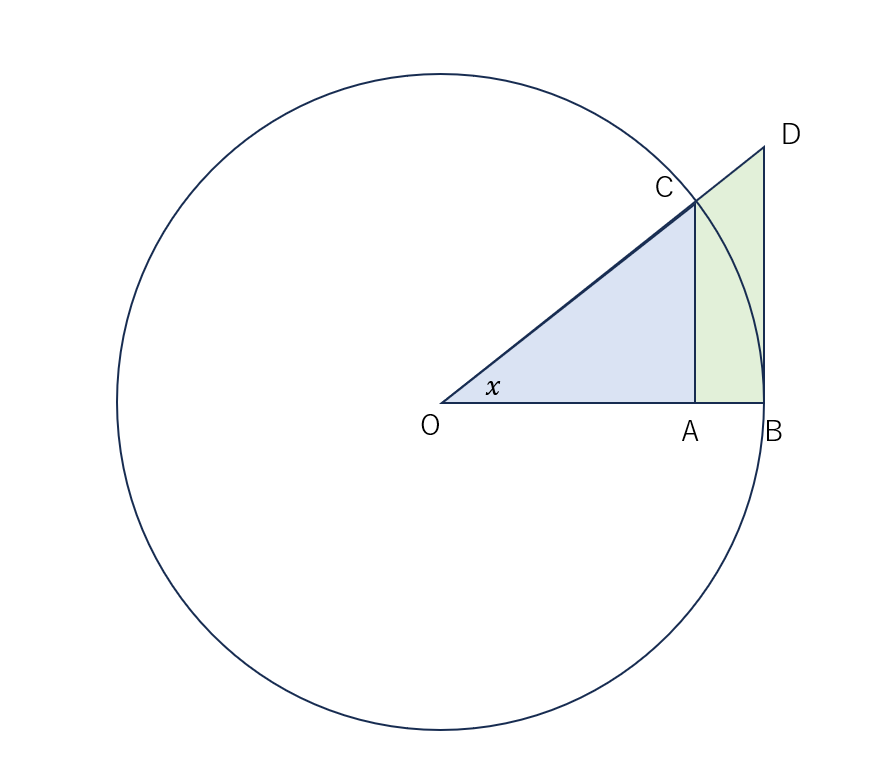
\includegraphics[keepaspectratio,scale=0.3]{img/QuuNote/circleFor_sin_div_xLimit.png}
                    \caption{単位円}
                \end{figure}

                このとき$\triangle OAC< OBC < \triangle OBD$である。それぞれ$\frac{1}{2}OA\cdot AC,\frac{1}{2}OC^2x,\frac{1}{2}OB\cdot BD$なので
                
                \begin{alignat}{3}
                    \frac{1}{2}OA\cdot AC&<& \frac{1}{2}OC^2x &<& \frac{1}{2}OB\cdot BD\notag\\
                    \frac{1}{2}OC^2 \sin x\cos x & < & \frac{1}{2}OC^2 x & < & \frac{1}{2}OC^2\tan x\notag\\
                    \sin x\cos x & < & x & < & \tan x\notag\\
                    \cos x & < & \frac{x}{\sin x} & < & \frac{1}{\cos x}\notag\\
                    \cos x & < & \frac{\sin x}{x} & < & \frac{1}{\cos x}\label{eq:Hasamiuti}
                \end{alignat}
                よって、$x\to 0$の極限を取れば$\displaystyle \cos x\to 1,\frac{1}{\cos x}\to 1$より$\displaystyle\frac{\sin x}{x}\to 1$となる。$\square$\footnote{より厳密な立場では、$x$が負の方向から近づく場合も考慮しなければならない。}\\

                最後の不等式\eqref{eq:Hasamiuti}のような不等式のとき、両側の極限値が一致すれば、間に挟まれた極限値も等しくなる。これを\textbf{はさみうちの原理}という。
                はさみうちの原理ではうまく挟み込める不等式をつくる必要があるので、慣れるまで時間がかかる。

            \clearpage
            \subsection{極限の計算}
                この節では実際に極限の計算方法について学ぶ。単純な場合は代入と同様に計算してよいが$\frac{0}{0}$などの形になる場合は式を変形する必要がある。

                \paragraph{例1}次の極限を求めよ。
                    \begin{equation*}
                        \lim_{x\to \infty}\frac{x^3+5x^2+x+2}{x^3+x+10}
                    \end{equation*}
                    $\frac{1}{x}\to 0(x\to \infty)$の結果を利用する。分子と分母に$\frac{1}{x^3}$をかけて
                    \begin{equation*}
                        \lim_{x\to \infty}\frac{1+\frac{5}{x}+\frac{1}{x^2}+\frac{2}{x^3}}{1+\frac{1}{x^2}+\frac{10}{x^3}}=\frac{1+0+0+0}{1+0+0}=1
                    \end{equation*}
                
                \paragraph{例2}次の極限を求めよ。
                    \begin{equation*}
                        \lim_{x\to 0}\frac{x}{1-\sqrt{x+1}}
                    \end{equation*}
                    $(a-b)(a+b)=a^2-b^2$を用いる。分子と分母に$1+\sqrt{x+1}$をかけて
                    \begin{equation*}
                        \lim_{x\to 0}\frac{x(1+\sqrt{x+1})}{(1-\sqrt{x+1})(1+\sqrt{x+1})}=\lim_{x\to 0}\frac{x(1+\sqrt{x+1})}{-x}=-(1+\sqrt{0+1})=-2
                    \end{equation*}
                
                \paragraph{例3}次の極限を求めよ。
                    \begin{equation*}
                        \lim_{x\to\infty}\frac{2^x+1}{3^x}
                    \end{equation*}
                    $x$が十分大きいとき$2^x\ll 3^x$であるため、直感的に極限値は0だとわかる。
                    \begin{equation*}
                        \lim_{x\to\infty}\left(\left(\frac{2}{3}\right)^x+\frac{1}{3^x}\right)=\lim_{x\to\infty}\left(\frac{2}{3}\right)^x+\lim_{x\to\infty}\frac{1}{3^x}=0+0=0
                    \end{equation*}
                    二項目は指数関数の性質$a^x\quad(a<1)$の場合を用いた。三項目は$x\to\infty$のとき$3^x\to\infty$であることを用いた。

                \paragraph{例4}次の等式を証明せよ。
                    \begin{equation*}
                        \lim_{x\to \infty}\left(1+\frac{1}{x}\right)^x = \lim_{x\to 0}\left(1+x\right)^\frac{1}{x} 
                    \end{equation*}
                    $x=\frac{1}{t}$と置くと、$x\to\infty$で$t\to0$だから
                    \begin{equation*}
                        \lim_{x\to \infty}\left(1+\frac{1}{x}\right)^x = \lim_{t\to 0}\left(1+\frac{1}{\frac{1}{t}}\right)^\frac{1}{t}=\lim_{t\to\infty}(1+t)^\frac{1}{t}
                    \end{equation*}
                    よって等式が成り立つ。\\

                もちろんこれ以外にも極限の計算を行う際に用いるテクニックは存在するが、もう少し勉強を進めないと使うことができない。その時が来るまで楽しみにしていてほしい。
                なお、これらのテクニックのほとんどは数列の極限にも用いることができる。
            \clearpage
            \subsection{関数の連続}
                次に、関数の連続について考えていく。ひとまず定義から述べる。関数$f(x)$が$x=a$で\textbf{連続}であるとは、次の三つの条件を満たすことである。
                \begin{enumerate}
                    \item $f(a)$が定義されている。
                    \item $\displaystyle\lim_{x\to a}f(x)$が存在する。
                    \item $\displaystyle f(a)=\lim_{x\to a}f(x)$である。
                \end{enumerate}
                極限の場合は$x=a$で値が存在していなくてもよかったが、連続では$x=a$での値も必要となる。なお、これを$\varepsilon-\delta$風に書けば、
                \begin{screen}
                    任意の$\varepsilon>0$に対して、ある$\delta >0$が存在して、$|x-a|<\delta $のとき、$|f(x)-\delta|<\varepsilon$
                \end{screen}
                である。$0<|x-a|<\delta$でないことに注意されたい。

                連続の条件2について、極限が存在するとはどういうことなのか考えてみよう。関数の極限$x\to a$では、\underline{$x$をどのように$a$
                に近づけても同じ極限値を取る}必要がある。
                どのように近づけても、と言われて困るかもしれないが、単に$x>a$の点と$x<a$の点から近づける場合を考えておけばよい。\footnote{二変数関数になると少し事情は変わる。`xy平面上のどの点から'近づけても同じになる必要がある。}

                このうち、$x>a$の点から近づける場合、すなわち数直線の右側から近づける場合を$\displaystyle\lim_{x\to a+0}f(x)$と表し、\textbf{右側極限値}と呼ぶ。
                同様に$x<a$の点から近づける場合は$\displaystyle\lim_{x\to a-0}f(x)$と表し、\textbf{左側極限値}と呼ぶ。この右側極限値と左側極限値が等しくなる時、
                極限は存在し、その値は
                \begin{equation}
                    \lim_{x\to a}f(x)=\lim_{x\to a+0}f(x)=\lim_{x\to a-0}f(x)
                \end{equation}
                となる。

                関数$f(x)$がある区間$I$で連続であるとき、$f(x)$は$I$で\textbf{連続関数}であるという。例えば、$f(x)=\sin x$は区間$(-\infty,\infty)$で連続関数である。
                一般に、初等関数は値が定義される(無限大にならないなど)全ての$x$について連続である。

                関数がある区間で連続であるといったが、そもそも区間の端での連続はどう定義すればよいだろうか。
                例えば、関数$f(x)=\sqrt{x}$は明らかに$x\geq 0$のすべての$x$で定義されているが$x=0$において連続の条件
                が適用できない。そこで、一般に関数が$x\geq a$で定義されているとき
                \begin{equation}
                    \lim_{x\to a+0}f(x)=f(a)
                \end{equation}
                が成り立てば、$x=a$において連続であるとする。こう定義することで、$\sqrt{x}$が区間$x\geq 0$で連続と定義できる。
                同様にして$x\leq b$である場合の端でも連続が定義される。この場合
                \begin{equation}
                    \lim_{x\to b-0}f(x)=f(b)
                \end{equation}
                のように左極限を取ることに注意。\\

                以下連続関数の性質について述べる。まず連続関数$f(x),g(x)$について
                \begin{equation}
                    f(x)\pm g(x)\quad f(x)g(x)\quad \frac{f(x)}{g(x)}
                \end{equation}
                は連続関数である。ただし、最後の式は$g(x)\neq 0$であるとする。このことから、連続関数の多項式も連続関数であることがわかる。\\

                \noindent
                例えば、$f(x)=x^n(n\in\mathbb{N})$は区間$(-\infty,\infty)$で連続であるため、多項式
                \begin{equation}
                    P(x)=a_nx^n+a_{n-1}x^{n-1}+\cdots+a_{1}x+a_0
                \end{equation}
                も区間$(-\infty,\infty)$で連続である。ほかにも、以下の\textbf{有理関数}
                \begin{equation}
                    R(x)=\frac{a_nx^n+a_{n-1}x^{n-1}+\cdots+a_{1}x+a_0}{b_nx^n+b_{n-1}x^{n-1}+\cdots+b_{1}x+b_0}
                \end{equation}
                も分母が0にならない限り連続である。

                また、次の\textbf{合成関数}$f(g(x))$を考えてみると、$f(x),g(x)$が連続関数であるかぎり$f(g(x))$も連続関数である。
                例えば$\log(\sqrt{x}+1)$は$x\geq 0$のすべての$x$で連続である。\\

                関数$f(x)$が区間$[a,b]$で連続関数である場合、次の二つが成り立つ。
                \begin{screen}
                    $f(a)\neq f(b)$なら$f(a)\leq k \leq f(b)$である任意の$k$について
                    \begin{equation*}
                        f(c)=k \label{eq:中間値の定理}
                    \end{equation*}
                    となる点$c\in[a,b]$が少なくとも一つ存在する。(\textbf{中間値の定理})
                \end{screen}
                \begin{screen}
                    $f(x)$は区間$[a,b]$で必ず最大値$M$と最小値$m$を取る。つまり
                    \begin{equation*}
                        m=f(x_m)\leq f(x)\leq f(x_M)=M
                    \end{equation*}
                    となる点$x_m,x_M\in[a,b]$が必ず存在する。
                \end{screen}
                文字だけだとわかりずらいが、グラフを見ればむしろ当たり前のことのように感じる。
                \begin{figure}[h]
                    \centering
                    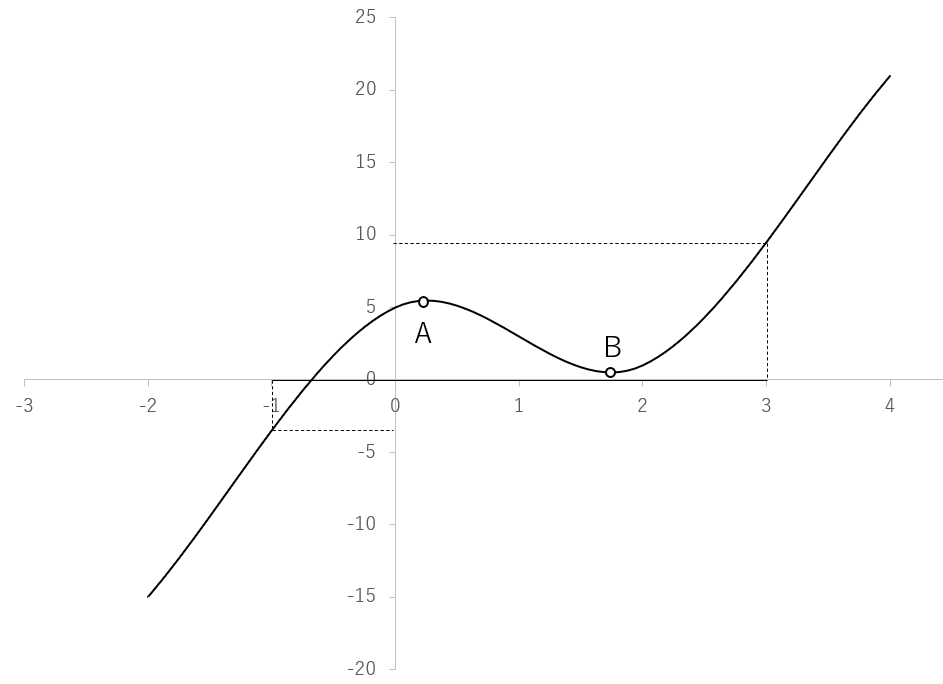
\includegraphics[keepaspectratio,scale=0.3]{img/QuuNote/ContinuousFuncGraph.png}
                    \caption{連続関数}\label{fig:連続関数,中間値の定理,最大最小}
                \end{figure}

                図\ref{fig:連続関数,中間値の定理,最大最小}を見ると、区間$[1,3]$において関数は連続であり、その端での値
                おおよそ$-3$と$9$の間のすべて値に対して、対応する$x\in[-1,3]$が存在していることがわかる。これが中間値の定理
                の主張である。また区間における最大値と最小値も存在している(それぞれ$x=-1,3$の点)ことがわかる。
                ちなみに、点A,Bはそれぞれその周囲の点の間では最大・最小の値である。これらをそれぞれ極大値、極小値とよび、総称して
                \textbf{極値}という。
                \newpage
                また、中間値の定理において$f(a)$と$f(b)$の符号が異なる場合、方程式$f(x)=0$は
                区間$[a,b]$に実数解を少なくとも持つことがわかる。\footnote{注:実数解を(少なくとも一つ)もつことは中間値の定理からわかるが、実数解を持たないことは中間値の定理ではいえない。例えば$f(x)=x^2,[-1,2]$では$f(-1),f(2)>0$であるが区間内に実数解をもつ。}これは中間値の定理の応用である。
                \paragraph{例}方程式$x^3-3x-1=0$は区間$[0,2]$に少なくとも一つの実数解を持つかどうか答えよ。

                $f(0)=0-0-1=-1<0,f(2)=8-6-1=1>0$より、$f(0)$と$f(2)$の符号が異なるため方程式は区間$[0,2]$で少なくとも一つの実数解をもつ。\\

                いままでは連続関数の性質について述べたが、連続の条件が一つでも満たされていない場合についても考えてみよう。
                このとき関数$f(x)$は$x=a$で\textbf{不連続}であるという。例えば$\frac{1}{x}$は$x=0$で不連続である。
                一方で関数$\displaystyle g(x)=\frac{x^2-1}{x-1}$も$x=1$で不連続であるが、$x\neq1$では$g(x)=x+1$で連続である。
                そこで、
                \begin{equation}
                    g(x)=\left\{\begin{array}{lr}\displaystyle\frac{x^2-1}{x-1}&(x\neq 1)\\ x+1&(x=1)\end{array}\right.
                \end{equation}
                のように改めて定義しなおすことで、この関数は$x=1$で連続にできる。各自確かめてみよ。
            \clearpage
            \basicquestion 以下の問いに答えよ。

                \paragraph{問1}以下の数列の一般項を示し、それらが収束するかどうか答えよ。\\
                $(1)\{a_n\}=\frac{2}{1},\frac{3}{2},\frac{4}{3}\cdots$\hspace{3mm}
                $(2)\{b_n\}=\frac{1}{3},\frac{1}{9},\frac{1}{27}\cdots$\hspace{3mm}
                $(3)\{c_n\}=1,-1,1,-1\cdots$\\
                $(4)\{d_n\}=a,a+d,a+2d,a+3d\cdots(a,dは定数)$

                \paragraph{問2}以下を証明せよ。
                \begin{equation*}
                    \lim_{n\to\infty}(a_n+b_n)=a+b
                \end{equation*}
                ただし、$\displaystyle\lim_{n\to\infty}a_n=a,\lim_{n\to\infty}b_n=b$とする。{\scriptsize ヒント:$\varepsilon-N$論法を用いる。}

                \paragraph{問3}以下計算せよ。\\

                \noindent
                $(1)\displaystyle \lim_{x\to 0}\frac{\sin2x}{x}$\hspace{3mm}
                $(2)\displaystyle \lim_{x\to 2\pi}\sin \frac{x}{2}+x^2$\hspace{3mm}
                $(3)\displaystyle \lim_{x\to\infty}\frac{x^2+x+1}{x^3+1}$\hspace{3mm}
                $(4)\displaystyle \lim_{x\to 0}\frac{x^2}{1-\cos x}$\hspace{3mm}
                $(5)\displaystyle \lim_{x\to 0}\tan x$\hspace{3mm}
                $(6)\displaystyle \lim_{x\to\infty}\frac{2^x+3^x}{2^x-3^x}$\\
                $(7)\displaystyle \lim_{x\to 0}\frac{\sqrt[3]{8+x}-2}{x}$\hspace{3mm}
                $(8)\displaystyle \lim_{x\to 0}\frac{e^x-1}{x}$
                
                \paragraph{問4}次の関数が()内の点において連続であるかどうか調べよ。\\
                $(1)f(x)=x^2\quad(x=2)$\hspace{1mm}
                $(2)f(x)=\sin x\quad(x=\frac{\pi}{2})$\hspace{1mm}
                $(3)f(x)=\sqrt{1-x^2}\quad(x=1)$\hspace{1mm}
                $(4)f(x)=\frac{1}{\sqrt{x}}\quad(x=0)$\\
                $(5)f(x)=|x|\quad(x=0)$\hspace{1mm}
                $(6)\displaystyle f(x)=\left\{\begin{array}{lr}\displaystyle x\sin\frac{1}{x}&(x\neq 0)\\1&(x=0)\end{array}\right.$\\

                \paragraph{問5}方程式$\sin x=x$が区間$[0,\frac{\pi}{2}]$に実数解をもつかどうか調べよ。
            \clearpage
            \section{第I部演習問題}
                \paragraph{問1} 以下の計算をせよ。ただし$(2)$において$-1<x<1$とする。
                    \begin{alignat*}{9}
                        &[1]\log\sqrt{2+\sqrt{3}} &[2]&\sin^{-1}x+\cos^{-1}x &[3]&\cos\left(\frac{5\pi}{12}\right) & [4]&\log(e^{x^2}) & [5]&\sin(12\pi)\\
                        &[6]\lim_{x\to 0}x^n(n\in\mathbb{N}) &[7]&\lim_{n\to 0}x^n &[8]&\lim_{n\to 0}(\sqrt{n^2+3n}-n) &[9]&\lim_{n\to\infty}(\sqrt[3]{n+1}-\sqrt[3]{n}) & [10]&\lim_{x\to \infty}\tanh x\\
                        &[11]\lim_{x\to +0}\frac{\sin x}{\sqrt{x}} &[12]& \lim_{x\to\infty}\frac{\sin(x)}{x} &[13]&\lim_{n\to\infty}\sum_{k=1}^{n}\left(\frac{k}{n}\right)\cdot \frac{1}{n} &[14]&\lim_{t\to 0}\frac{(x+t)^2-x^2}{t}
                    \end{alignat*}
                \paragraph{問2}次の式について以下の問いに答えよ。
                    \begin{equation}
                        \lim_{n\to n}a_n=a \Rightarrow \lim_{n\to\infty}\frac{a_1+a_2+\cdots+a_n}{n}=a
                    \end{equation}
                    \begin{description}
                        \item[(1\textrm{)}] 上式を証明せよ。
                        \item[(2\textrm{)}] $\log\left(\frac{2}{1}\times\frac{3}{2}\times\cdots\times\frac{n+1}{n}\right)-\log\frac{n+1}{n}$を求めよ。
                        \item[(3\textrm{)}] $\displaystyle \lim_{n\to\infty}\frac{\log n}{n}$を求めよ。
                    \end{description}
                
                \paragraph{問3}
                    次の関数が$[\quad]$の点で連続であるかどうか答えよ。
                    \begin{align*}
                        (1)&\sign x = \left\{\begin{array}{cc}\displaystyle 1 & (x>0) \\ 0 & (x=0) \\ -1 & (x<0)\end{array}\right.&\quad [x=0]\\
                        (2)&f(x)=\lim_{n\to \infty}f_n(x)\quad (f_n(x)=x^n\quad(0\leq x\leq 1))&\quad [x=1]
                    \end{align*} 
                    (1)の関数は\textbf{符号関数}という。${\rm sgn}(x)$と書く場合もある。

                \paragraph{問4}
                    数学において$0^0$は$1$と定義されたりそもそも定義されなかったりする。さて、$0^0=1$と定義する立場での根拠について関数$f(x)=x^x$を用いて極限の観点から述べよ。
                
                \linktoMOKUZI
                
    \clearpage
    \part{微分法$f'$}
    \vspace{\stretch{1}}
    \begin{screen}
        いよいよ微分積分の``微分''の話に移る。微分法は、関数の挙動について解析するときに用いる。具体的な計算は公式に当てはめるだけなので
        そこまで難しくない。それにもかかわらず微分の応用例は幅広い。理屈がわかったらあとは練習あるのみである。
        また、ここではテイラー展開などについても扱う。
    \end{screen}
    \clearpage
    \section{導関数}
        \subsection{平均変化率・微分係数}
            一次関数$y=\alpha x+b$の傾き$\alpha$を求める方法は直線上の二点の座標がわかればよく、それらを$(x_1,y_1),(x_2,y_2)$と置けば、
            \begin{equation}
                \alpha=\frac{y_2-y_1}{x_2-x_1}
            \end{equation}
            で求まる。また分子と分母はそれぞれ$(x_1,y_1)$からの$x$方向$y$方向の変化分だと考えられるので、それらを$\Delta x=x_2-x_1,\Delta y=y_2-y_1$と置けば
            \begin{equation}
                a= \frac{\Delta y}{\Delta x}
            \end{equation}
            となる。これを一般の関数$y=f(x)$に拡張することを考える。ここで注意しておいてほしいのは、
            一般の関数で考える際は$(x_1,y_1),(x_2,y_2)$の取り方によって傾きの値が変わってしまうことである。

            例えば、$y=x^2$について$(1,1^2)$から$(2,2^2)$の傾きは$\frac{4-1}{2-1}=3$だが、
            $(3,3^2)$から$(4,4^2)$の傾きは$\frac{16-9}{4-3}=7$となってしまう。つまり$x$の増分が同じであっても
            $y$の増分が同じであるとは限らないのである。

            とはいえ、傾きの式を$y=f(x)$の場合で拡張するからなにか定義の式が変わるわけではない。やはり二点の座標について
            \begin{equation}
                \frac{f(x_2)-f(x_1)}{x_2-x_1}\quad\left(=\frac{y_2-y_1}{x_2-x_1}\right)
            \end{equation}
            となる。この$x$の増分と$y$の増分の比のことを\textbf{平均変化率}という。
            \begin{figure}[h]
                \centering
                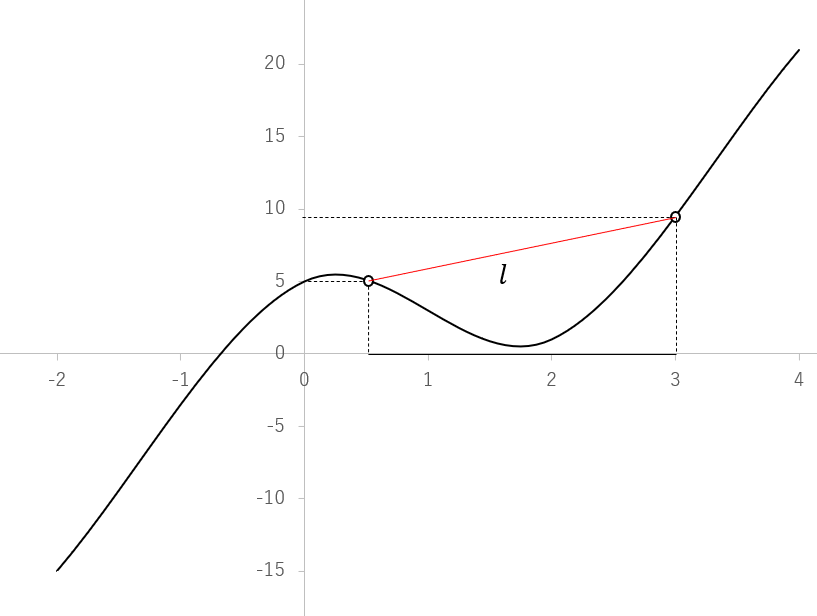
\includegraphics[scale=0.3]{img/QuuNote/heikinhenkaritu.png}
                \caption{平均変化率と直線}
            \end{figure}

            上図のように、平均変化率は二点を結んだ直線$l$の傾きを表している。また$a=x_1,b=x_2$と置き、$a$と$b$の差を$h=b-a$と置けば、
            \begin{equation}
                \frac{f(a+h)-f(a)}{h}
            \end{equation}
            と表すこともできる。
            
            次に点$x=b$を点$x=a$に限りなく近づける場合を考えよう。これは$a$と$b$との距離が限りなく小さくなることを意味するので$h\to 0$の極限である。すなわち
            \begin{equation}
                \lim_{h\to 0}\frac{f(a+h)-f(a)}{h}
            \end{equation}
            となる。この極限値が存在する場合、$f(x)$は$x=a$で\textbf{微分可能}であるという。また、その値を$x=a$における$f(x)$の\textbf{微分係数}といい、$f'(a)$と表す。
            \clearpage
            $h$は右側(正の側)から0に近づく場合と左側(負の側)から0に近づく場合がある。
            前者を\textbf{右方微分係数}といい
            \begin{equation}
                f'(a+0)=\lim_{h\to +0}\frac{f(a+h)-f(a)}{h}
            \end{equation}
            と表す。同様に後者を\textbf{左方微分係数}といい
            \begin{equation}
                f'(a-0)=\lim_{h\to -0}\frac{f(a+h)-f(a)}{h}
            \end{equation}
            と表す。微分可能とは$f'(a+0)$と$f'(a-0)$が存在して、$f'(a+0)=f'(a-0)$となることと同義である。
            もし$f(x)$が$x\geq a$で定義されている場合は、$x=a$における右方微分係数が存在していればよく、$x\leq a$で定義されている場合は左方微分係数が存在していればよい。
            \\

            では次に微分係数の幾何学的な意味について考えていこう。そのためには$b$を$a$に徐々に近づけた場合の$a-b$を結ぶ直線を書くとわかりやすい。
            \begin{figure}[h]
                \centering
                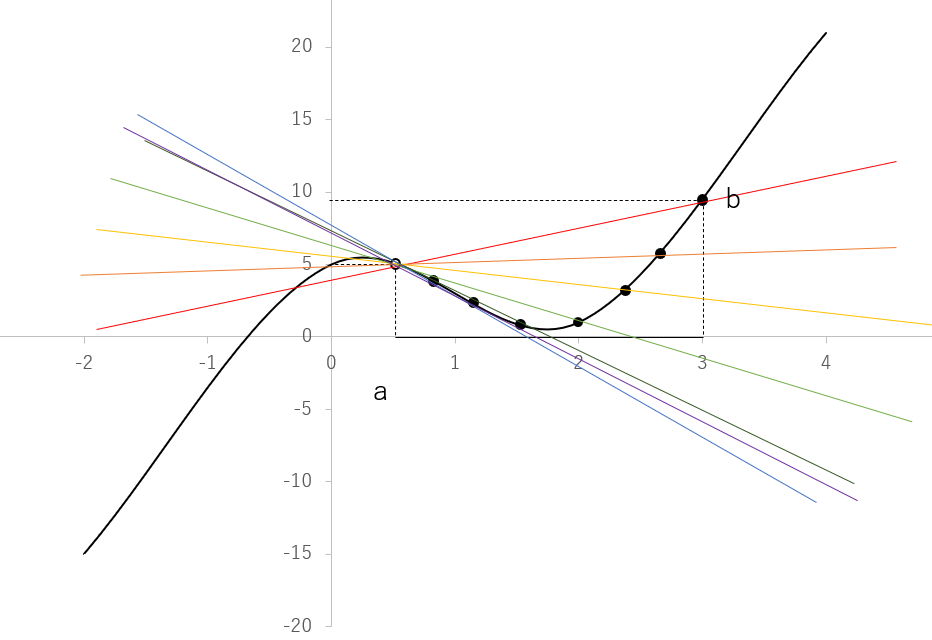
\includegraphics[scale=0.5]{img/QuuNote/differentialCoefficieant_Graph.png}
                \caption{点$b$を徐々に近づけた場合の直線の変化}
            \end{figure}

            この図を見ると$b$が$a$に近づくにつれて、二点を結んだ直線も点$a$の\textbf{接線}に近づいていることがわかる。
            つまり$x=a$における微分係数は点$a$の接線の傾きを表している。
        \clearpage
        \subsection{微分可能性と連続性}
            今度は関数が$f(x)$が$x=a$で微分可能であることと連続であることの違いについて考えていこう。
            一見するとこれら二つは同値であるかのように見える。\footnote{昔の数学者たちの間でも長らく連続関数は明らかに微分可能と考えられていたらしい。だからこそワイエルシュトラスの$W(x)$関数
            のような連続なのにいたるところで微分不可能な関数が発見されたときは、数学界に大きな衝撃を与えたそうだ。\\参考書籍:\url{https://www.iwanami.co.jp/book/b480065.html}}
            実際初等関数は連続である区間についてすべて微分可能である。では初等関数ではない関数である$y=|x|$で考えてみよう。
            もちろん$x>0$では$y=x$、$x<0$では$y=-x$であるので、微分可能である。(実際に試すとよい)
            しかし$x=0$においては微分可能ではない。\footnote{幾何学的に言えば接線が二本引けてしまうことが理由となる。つまり微分可能性とはその点においてただ一つ接線が引けることと理解できる。\label{微分可能性の幾何学的意味}}それを今から示す。

            微分可能であることは、右方微分係数と左方微分係数が一致すればよいことであるが
            \begin{equation}
                \frac{|0+h|-|0|}{h}=\frac{|h|}{h}
            \end{equation}
            なので、
            \begin{align}
                y'(+0)&=\lim_{h\to +0}\frac{|h|}{h}=\lim_{h\to+0}\frac{h}{h}=1\\
                y'(-0)&=\lim_{h\to -0}\frac{|h|}{h}=\lim_{h\to -0}\frac{-h}{h}=-1
            \end{align}
            となり右方微分係数と左方微分係数が一致しない。したがって$y=|x|$は$x=0$で微分可能ではないので、
            $y=|x|$は連続であるが微分可能でない関数であることがわかる。

            では逆に$f(x)$が$x=a$で微分可能であるときはどうであろうか。$f(x)$が$x=a$で微分可能であるとき
            \begin{equation}
                \lim_{h\to 0}(f(a+h)-f(a))=\lim_{h\to 0}\frac{f(a+h)-f(a)}{h}\cdot h=\lim_{h\to 0}f'(a)\cdot h=0 
            \end{equation}
            また、$\displaystyle \lim_{h\to 0}(f(a+h)-f(a))=\lim_{h\to 0}f(a+h)-\lim_{h\to 0}f(a)=\lim_{h\to 0}f(a+h)-f(a)$なので、
            \begin{equation}
                \lim_{h\to 0}f(a+h)=f(a)
            \end{equation}
            が成り立つ。$h=b-a$であったことを思い出すと、$h\to 0$のとき$b\to a$なので
            \begin{equation}
                \lim_{b\to a}f(b) = f(a)
            \end{equation}
            つまり$x=a$で$f(x)$は連続の条件を満たす。\\\\
            \noindent
            以上をまとめると\fbox{$f(x)$が$x=a$で微分可能$\Rightarrow$$f(x)$は$x=a$で連続}である。 \\

            ちなみに、$x=a$で$f(x)$が不連続である場合は、対偶を取ればわかるように微分可能ではない。これは微分係数の定義からもわかる。
        \clearpage
        \subsection{導関数の定義}
            関数$f(x)$の微分係数は$f'(a)$であり、これは$x=a$の点において$y=f(x)$上の接線の傾きを意味していることは前回学んだ。
            では次に任意の$x$の値に対して$f(x)$の接線の傾きを返す関数を考えてみよう。この間数は以下のように定義できる。
            \begin{equation}
                f'(x)=\lim_{h\to 0}\frac{f(x+h)-f(x)}{h}
            \end{equation}
            このような関数$f'(x)$を$f(x)$の\textbf{導関数}という。$x=a$のときの導関数の値が$f'(a)$であり、これは$x=a$の微分係数である。

            導関数には以下のような書き方がある。
            \begin{equation}
                \frac{dy}{dx},\quad\frac{df}{dx},\quad y',\quad f'(x),\quad\frac{d}{dx}y,\quad\frac{d}{dx}f(x),\quad D_xf(x),\quad Df(x)
            \end{equation}
            このうち$\frac{d}{dx}$\footnote{読み方は分子から。「でぃーわいでぃーえっくす」など。}の書き方はライプニッツ、$f',y'$の書き方はラグランジュによるものである。$D_x,D$はコーシーによる。
            ライプニッツの書き方は導関数の意味が明瞭であるが書く際に場所を取ってしまったりするので簡潔なラグランジュの書き方も使われる。(コーシーの書き方は演算子であることが明瞭である気がする。)このノートはどちらもその
            場合に応じて使い分けていく。
            ちなみに、変数が時間である場合など、物理関係では$\dot{x}(t)$などとして表すこともある。これはニュートンの書き方である。\\

            試しに、$f(x)=x$の導関数を求めてみる。
            \begin{equation}
                f'(x)=\lim_{h\to 0}\frac{f(x+h)-f(x)}{h}=\lim_{h\to 0}\frac{(x+h)-x}{h}=1
            \end{equation}
            したがって、$f(x)=x$の導関数は$f'(x)=1$であることがわかる。これは定数関数であるので$x$の値によらない。
            つまり$y=x$はどの点でも傾きが同じであることがわかる。実際グラフを想像すれば直線で傾きは一定である。\\

            一般に$f,g$が微分可能、$a=定数$であるとき以下の公式が成り立つ。
            \begin{alignat}{3}
                &(a)' &&= 0\\
                &(a f(x))' &&= af'(x)\\
                &(f(x)\pm g(x))' &&=f'(x)\pm g'(x)
            \end{alignat}
            どれも定義からすぐに導出できる。気になる人は試してみてほしい。
        \clearpage
        \basicquestion 以下の問いに答えよ。

            \paragraph{問1}次の関数の(\hspace{2mm})内の区間での平均変化率を求めよ。
            \begin{alignat*}{2}
                &(1)y=x^2+1 &&(x=1\to 3)\\
                &(2)y=x^3+x^2+x+1 &&(x=-1\to 1)\\
                &(3)y=\sin x &&(x=\frac{\pi}{6}\to\frac{\pi}{3})
            \end{alignat*}

            \paragraph{問2}次の関数を微分せよ。\\
            \noindent
            $(1)y=x+1$\hspace{5mm}
            $(2)y=5$\hspace{5mm}
            $(3)y=x^3$\hspace{5mm}
            $(4)y=ax+b$\hspace{5mm}
            $(5)y=a(x+p)^2+q$

            
            \paragraph{問3}$y=\sqrt{x}\hspace{1mm}(x\geq 0)$が微分可能であるか調べよ。

            \paragraph{問4}以下の式を証明せよ。
            \begin{equation*}
                \frac{d}{dx}(af(x))=a\frac{d}{dx}f(x)
            \end{equation*}
            ただし、$f(x)$が微分可能とする。
        \clearpage
        \section{導関数の計算}
            \subsection{基礎的な関数の導関数}
                \noindent
                ここでは初等関数の基礎的な関数$x^n,\sin x,e^x,\log x$などの導関数を求めていく。\\

                まず、$e^x$から考えてみよう。ひとまず定義に従えば
                \begin{equation}
                    \lim_{h\to 0}\frac{e^{x+h}-e^{x}}{h}=e^x\lim_{h\to 0}\frac{e^h-1}{h}
                \end{equation}
                と変形できる。そこで、出てきた極限について逆数をとり$t=e^h-1$とおいて計算していく。
                \begin{equation}
                    \lim_{h\to 0}\frac{h}{e^h-1}=\lim_{t\to 0}\frac{\log(t+1)}{t}=\lim_{t\to 0}\log(1+t)^\frac{1}{t}
                \end{equation}
                と変形できるので、$e$の定義式\eqref{eq:define_e}より真数は$e$となる。したがってこの極限は$1$となるので
                \begin{equation}
                    (e^x)'=e^x \cdot \lim_{h\to 0}\frac{e^h-1}{h}=e^x \cdot 1 =e^x
                \end{equation}
                つまり$e^x$は\underline{微分しても形が変わらない}のである。
                また、この結果を使えば一般の指数関数$a^x$の導関数も簡単に求まる。$(e^{ax})'=ae^{ax}$が成り立つ(演習問題)ことから
                \begin{equation}
                    (a^x)'=(e^{\log(a^x)})'=(e^{x\log a})'=e^{x\log a}\log a=a^x\log a
                \end{equation}

                つぎに、$\log x$について考えてみる。これも定義に従って
                \begin{equation}
                    \lim_{h\to 0}\frac{\log(x+h)-\log x}{h}=\lim_{h\to 0}\frac{\log\left(\frac{x+h}{x}\right)}{h}=\lim_{h\to 0}\log\left(1+\frac{h}{x}\right)^\frac{1}{h}
                \end{equation}
                ここで$t=\frac{h}{x}$と置けば
                \begin{equation}
                    \lim_{t \to 0}\log(1+t)^\frac{1}{xt}=\lim_{t\to 0}\frac{\log(1+t)^\frac{1}{t}}{x}=\frac{\log(e)}{x}=\frac{1}{x}
                \end{equation}
                と求まる。

                次に、$x^n$で求めてみよう。ただし$n$は自然数であるとする。一般に、
                \begin{equation}
                    (x+a)^n=x^n+{}_nC_1ax^{n-1}+{}_nC_2a^2 x^{n-2}+\cdots +{}_nC_ma^{m}x^{n-m}+\cdots {}_nC_1a^{n-1}x+a^n\quad(\text{\textbf{二項定理}})\label{eq:二項定理}
                \end{equation}
                が成り立つので
                \begin{alignat}{1}
                    (x^n)'&=\lim_{h\to 0}\frac{(x+h)^n-x^n}{h}=\lim_{h\to 0}\frac{{}_nC_1hx^{n-1}+{}_nC_2h^2 x^{n-2}+\cdots +{}_nC_mh^{m}x^{n-m}+\cdots +{}_nC_1h^{n-1}x+h^n}{h}\\
                    &=\lim_{h\to 0} {}_nC_1 x^{n-1}+(h\text{についての多項式})=nx^{n-1}
                \end{alignat}
                要するに$x^n$の微分は\underline{肩をおろして1を引く}のである。
                \clearpage
                最後に$\sin x$の導関数を求めてみよう。こちらも定義通りに計算して
                \begin{equation}
                    (\sin x)'=\lim_{h\to 0}\frac{\sin(x+h)-\sin x}{h}=\lim_{h\to 0}\frac{2\cos(\frac{2x+h}{2})\sin(\frac{h}{2})}{h}=\lim_{h\to 0}\cos (x+\frac{h}{2})\cdot \lim_{h\to 0}\frac{\sin\frac{h}{2}}{\frac{h}{2}}=\cos x
                \end{equation}
                最後の極限は式\eqref{eq:limit of sin/x}を利用した。\\

                これで基礎となる関数の導関数はほとんど導出できた。以下公式としてまとめる。一部導出していないものもあるが演習問題で導出する。これくらいは後々の計算のためにも覚えておくとよい。

                \begin{screen}
                    \begin{alignat*}{2}
                        &(x^n)'=nx^{n-1} && (a^x)'=a^x\log a\\
                        &(e^x)'=e^x && (\log x)'=\frac{1}{x}\\
                        &(\sin x)'=\cos x \quad&& (\cos x)'=-\sin x
                    \end{alignat*}
                \end{screen}
            \clearpage
            \subsection{積の微分}
                今度は 関数同士の積について、公式を導出してみよう。$f,g$は微分可能であるとする。このとき、
                \begin{equation}
                    (f(x)g(x))'=\lim_{h\to 0}\frac{f(x+h)g(x+h)-f(x)g(x)}{h}
                \end{equation}
                である。当然このままでは計算できないので少し式をいじってあげよう。仮定より分子にどうにかして$f(x+h)-f(x)$もしくは$g(x+h)-g(x)$
                を作れないか考えてみる。そこで分子に$-f(x+h)g(x)+f(x+h)g(x)=0$を加えてあげると
                \begin{equation}
                    \frac{f(x+h)(g(x+h)-g(x))+g(x)(f(x+h)-f(x))}{h}=\frac{f(x+h)(g(x+h)-g(x))}{h}+\frac{g(x)(f(x+h)-f(x))}{h}
                \end{equation}
                とできる。あとは$f,g$が微分可能であるので$h\to  0$の極限を取れば
                \begin{equation}
                    (f(x)g(x))'=f(x)g'(x)+f'(x)g(x)\label{eq:積の微分公式}
                \end{equation}
                こうして積の微分公式が得られた。では、この公式を用いて$\displaystyle y=x^{-n}=\frac{1}{x^{n}}$の導関数も求めてみよう。
                \begin{equation}
                    (1)'=\left(\frac{x^n}{x^{n}}\right)'=nx^{n-1}\cdot \frac{1}{x^{n}}+x^n\cdot \left(\frac{1}{x^n}\right)'=\frac{n}{x}+x^{n}y'=0
                \end{equation}
                であるため、$y'=$の形に整理すれば
                \begin{equation}
                    y'=\frac{-n}{x^{n+1}}=(-n)\cdot x^{(-n)-1}\label{eq:積微分による1/x^nの微分}
                \end{equation}
                つまり、任意の整数について$(x^n)'=nx^{n-1}$が成り立つことが示せた。\footnote{この例は積の微分公式を使う練習としてはあまり適していない。商の微分を用いるか合成関数の微分法を用いることで見通しよく求められる。}\\

                もう少し簡単な問題で積の微分公式を使う練習をしてみよう。
                \paragraph{例題}$y=x\sin x$のとき$y'$を求めよ。\\
                $f=x,g=\sin x$とおいて式\eqref{eq:積の微分公式}を適応すると$f'=1,g'=\cos x$だから
                \begin{equation}
                    y'=fg'+f'g=x\cos x+\sin x
                \end{equation}
                と求まる。
            \clearpage
            \subsection{商の微分}
                積の微分について考えたら次は商の微分についても考えたくなるものである。商の微分公式について以下にのべる。
                \begin{equation}
                    \left(\frac{f(x)}{g(x)}\right)'=\frac{f'(x)g(x)-f(x)g'(x)}{\left\{g(x)\right\}^2}\label{eq:商の微分公式}
                \end{equation}
                もちろん$f,g$は微分可能であり$g(x)\neq 0$であるとする。頭の痛くなる形をしていて、覚えるのに苦労しそうである。
                覚え方は人によってさまざまだろうが、例えば「分子は積の微分の符号反転で分母は二乗する」という覚え方もある。導出については
                演習問題とする。

                商の微分について$f=1$の特別な場合を知っておくと計算が早くなることがある。試しに公式に代入してみると
                \begin{equation}
                    \left(\frac{1}{g}\right)'=\frac{0\cdot g-1\cdot g'}{g^2}=-\frac{g'}{g^2}
                \end{equation}
                となる。最後の符号を忘れないように注意しよう。ここまで覚える必要はないが知っておけば多少楽できる。\\

                ではこれを使って$y=x^{-n}$の導関数を導出してみよう。$f=1,g=x^n$として公式に代入すればよい。
                \begin{equation}
                    y'=-\frac{(x^n)'}{(x^n)^2}=-\frac{nx^{n-1}}{(x^n)^2}=-\frac{n}{x^{n+1}}=(-n)\cdot x^{(-n)-1}
                \end{equation}
                となり、式\eqref{eq:積微分による1/x^nの微分}と同じ結果が得られた。こちらの方が自然な導出である。

                次に$y=\tan x$の導関数を導出してみよう。この関数は$\sin x$などと違って定義から計算すると骨が折れる。しかし、商の微分公式を用いれば
                \begin{equation}
                    y'=\left(\frac{\sin x}{\cos x}\right)'=\frac{\cos^2 x-(-\sin^2 x)}{\cos^2 x}=\frac{1}{\cos^2 x}
                \end{equation}
                と楽に導出できる。
            \clearpage
            \subsection{合成関数の微分}
                では次に合成関数の微分について考えてみる。$y=f(g(x))$として考えてみる。このとき
                \begin{equation}
                    y'=\lim_{h\to 0}\frac{f(g(x+h))-f(g(x))}{h}=\lim_{h\to 0}\frac{f(g(x+h))-f(g(x))}{g(x+h)-g(x)}\cdot \frac{g(x+h)-g(x)}{h}
                \end{equation}
                であるので、$h'=g(x+h)-g(x)$と置けば、$h\to 0$で$h'\to0$なので、
                \begin{equation}
                    \lim_{h'\to 0}\frac{f(g(x)+h')-f(g(x))}{h'}\cdot \lim_{h\to 0}\frac{g(x+h)-g(x)}{h}=f'(g(x))\cdot g'(x)
                \end{equation}
                となる。$u=g(x)$とおいてこれをライプニッツの記号で書けば
                \begin{equation}
                    \frac{dy}{dx}=\frac{dy}{du}\frac{du}{dx}\label{eq:合成関数の微分}
                \end{equation}
                こうすれば`形式的に'約分しているように見ることができる。ちなみにこの合成関数の微分の公式を\textbf{チェイン・ルール}という。
                
                合成関数の微分公式を用いれば一般の$m$について$(x^m)'=mx^{m-1}$が証明できる。それを今から示す。\footnote{これは対数微分法でも示せる。そもそも対数微分法も今回のやり方も本質的には同じである。}
                \begin{equation}
                    (x^m)'=(e^{\log x^m})'=(e^{m\log x})'=e^{m\log x}\cdot (m\log x)'=x^{m}\cdot \frac{m}{x}
                \end{equation}
                と計算できるので、
                \begin{equation}
                    (x^m)'=mx^{m-1}
                \end{equation}
                
                ほかにも$(2x+1)^5$を微分するとき、通常なら展開して項別微分する必要があるが、合成関数を用いれば
                \begin{equation}
                    \left\{(2x+1)^5\right\}'=5(2x+1)^4\cdot (2x+1)'=10(2x+1)^4
                \end{equation}
                と非常に簡単に求められる。より一般的には
                \begin{equation}
                    (f(ax+b))'=af'(ax+b)
                \end{equation}
                である。
            \clearpage
            \subsection{逆関数の微分}
                前回までで和・差・積・商のすべての場合について、微分の公式を導入した。これさえあればどんな関数でも微分できそうであるが、実はそうではない。
                例えば$\arcsin x$は、$\sin x$の逆関数であること以外何も関数についてわかっていない。このような関数の微分について考えよう。

                まず、一価単調連続関数$f(x)$について、逆関数を$y=f^{-1}(x)$と表すことにすれば、導関数の定義より
                \begin{equation}
                    \lim_{h\to 0}\frac{f^{-1}(x+h)-f^{-1}(x)}{h}
                \end{equation}
                ここで$y=f^{-1}(x)$と置くと、$x=f(y)$である。また、$Y=f^{-1}(x+h)$と置けば$x+h=f(Y)$である。したがって$h=f(Y)-f(y)$である。$h\to 0$のとき$Y\to y$だから$h'=Y-y$と置けば$h'\to 0$である。
                \begin{equation}
                    \lim_{h'\to 0}\frac{h'}{f(y+h')-f(y)}=\lim_{h'\to 0}\frac{1}{\displaystyle\frac{f(y+h')-f(y)}{h'}}
                \end{equation}
                ここで$f(x)$が微分可能であるとすれば、この極限は収束して
                \begin{equation}
                    \frac{dy}{dx}=\frac{1}{\displaystyle\frac{dx}{dy}}\label{eq:逆関数の微分公式}
                \end{equation}
                となる。これが逆関数の微分公式である。形式的には$dy,dx$を一つの量とみなして変形した形と一致する。\\

                ではこの公式を用いて件の$\arcsin x$を求めてみることにしよう。$y=\arcsin x$とすれば当然$x=\sin y$であるから、
                \begin{equation}
                    \frac{dy}{dx}=\frac{1}{\displaystyle\frac{dx}{dy}}=\frac{1}{\displaystyle\frac{d}{dy}\sin y}=\frac{1}{\cos y}=\frac{1}{\sqrt{1-\sin^2 y}}=\frac{1}{\sqrt{1-x^2}}
                \end{equation}
                と求まった。つぎに$y=\log x$について、公式を適用してみよう。逆関数が$e^x$であることに注意すれば
                \begin{equation}
                    \frac{dy}{dx}=\frac{1}{\frac{d}{dy}e^{y}}=\frac{1}{e^y}=\frac{1}{x}
                \end{equation}
                となり、公式が正しいことも確認できる。
            \clearpage
            \subsection{微分}
                ここでは微分という概念について述べる。突然だが微分可能な関数$f$について$y=f(x)$のグラフを考えてみる。この時グラフ上の点$(x,y)$
                は、必ず接線を持つはずである。\footref{微分可能性の幾何学的意味}このとき、その接線上の点$(X,Y)$について$dx=X-x,dy=Y-y$となるような
                座標の変動$dx,dy$を定義してあげると
                \begin{equation}
                    dy=f'(x)dx
                \end{equation}
                は、点$(x,y)$の接線の方程式と全く同じものであることがわかる。この時$dx=\Delta x$とすると、
                グラフ上の座標の変動$\Delta y$は必ずしも$dy$と等しくはならない。このような$dx,dy$をそれぞれ$x,y$の\textbf{微分}という。\\

                これらの意味するところについて述べたいのはやまやまだが、ここでは記号的な話にのみ焦点を当てる。形式的な話であるので得られた結果が正しい可能性はないし、
                そもそもここからすべての導関数が導出できるわけではないだろうが、便利なので紹介する。

                まずは、演算の規則について、次の三つがある。
                \begin{enumerate}
                    \item $dy=f'(x)dx$
                    \item $d(u\pm v)=du\pm dv$
                    \item $d(uv)=vdu+udv$
                \end{enumerate}
                
                これを用いて一つ導関数を求めてみよう。例えば陰関数$F(x,y)=x^2+y^2-r^2=0$について、$\frac{dy}{dx}$を求めてみることにする。まず、$x,y$を両辺に分け、それぞれ$d$(ディー)して
                \begin{equation}
                    d(x^2-r^2)=d(y^2)
                \end{equation}
                演算の規則2より、$d(x^2-r^2)=d(x^2)-d(r^2)$と分けられる。この時、$r$は$x,y$によらないと考えているので$d(r^2)=0$である。よって、
                \begin{equation}
                    2xdx=2ydy
                \end{equation}
                式を変形すると、
                \begin{equation}
                    \frac{dy}{dx}=\frac{x}{y}
                \end{equation}
                となる。まるで魔法にかけられたみたいにあっさり求まってしまったが、この結果は正しいのだろうか?試しに$y>0$として元の式を変形すると$y=\sqrt{r^2-x^2}$となる。
                このとき、$x$微分すると
                \begin{equation}
                    \frac{dy}{dx}=\frac{x}{\sqrt{r^2-x^2}}=\frac{x}{y}
                \end{equation}       
                と確かに一致することがわかる。        
            \clearpage
            \basicquestion 以下の問いに答えよ。
            
                \paragraph{問1}以下の関数の導関数を求めよ。\\
                $(1)y=x^2+1$\hspace{3mm}
                $(2)y=\cos x+\sin x$\hspace{3mm}
                $(3)y=\log 2x$\hspace{3mm}
                $(4)y=\cos^{-1}x$\hspace{3mm}
                $(5)y=e^{\tan x}$\hspace{3mm}
                $(6)y=e^{x^2}\cos 2x$\\
                $\displaystyle(7)y=\log(x+\sqrt{x^2+1})$\hspace{3mm}
                $(8)y=f^{-1}(x)\quad (f(x)=x^3)$

                \paragraph{問2}以下を示せ。\\
                (1)商の微分公式\eqref{eq:商の微分公式}を示せ。\\
                (2)$(e^{ax})'=ae^{ax}$を導関数の定義から導出せよ。\\
                (3)$\cos x$の導関数を$\sin^2 x+\cos ^2 x=1$の関係を利用して導出せよ。ただし$\cos x\neq 0$であるとする。

                \paragraph{問3}以下の関数の導関数を工夫して求めよ。\\{\scriptsize ヒント:(1)(2)両辺対数を取るか$e^{\log f(x)}$の形にせよ。(3)普通に解いてもよいが$x=\tan \theta$と置いて合成関数の微分公式を用いると楽に出せる。}\\
                $\displaystyle(1)y=\sqrt[3]{\frac{x^2+1}{(x+1)^2}}\quad(x>-1)$\hspace{3mm}
                $(2)y=x^x$\hspace{3mm}
                $\displaystyle(3)y=\sin^{-1}\frac{x}{\sqrt{1+x^2}}$

                \paragraph{問4}双曲線関数について、$\sinh x,\cosh x$の導関数を導出せよ。

                \paragraph{問5}以下の公式について、後の問いに答えよ。
                \begin{eqnarray}
                    \sin\alpha\cos\beta=\frac{1}{2}\left\{\sin(\alpha+\beta)+\sin(\alpha-\beta)\right\}\label{eq:和積の公式sinαcosβ}
                \end{eqnarray}
                \begin{enumerate}\setcounter{enumi}{0}\renewcommand{\labelenumi}{(\arabic{enumi})}
                    \item 公式\eqref{eq:和積の公式sinαcosβ}を示せ。
                    \item 公式\eqref{eq:和積の公式sinαcosβ}の両辺を$\alpha$微分せよ。
                    \item 公式\eqref{eq:和積の公式sinαcosβ}の両辺を$\beta$微分せよ。
                \end{enumerate}
                
            \clearpage
            \section{微分法の応用}
                \subsection{関数の増減}
                    この節からは微分法の応用について述べる。まずは、微分法を用いて関数の増減について調べていこう。ひとまず
                    微分係数が何を示しているかを復習しておくと、これは$y=f(x)$のグラフにおいてその点の接線の傾きを示しているのだった。
                    傾きの大きさ(度合い)は一旦無視してその符号にのみ着目すると、傾きが正であるとき(一次関数のグラフと同様)その点周辺で$f(x)$は増加しており
                    逆に負の場合は減少していることがわかる。すなわち次の結果が得られる。
                    \begin{screen}
                        ある$x$の区間$I$について
                        \begin{itemize}
                            \item $f'(x)>0$である場合は$y=f(x)$は区間$I$で\underbar{単調増加}
                            \item $f'(x)<0$である場合は$y=f(x)$は区間$I$で\underbar{単調減少}
                        \end{itemize}
                        が成り立つ。
                    \end{screen}
                    例えば、$y=x^2$は$(x^2)'=2x$なので、$x>0$で単調増加しており$x<0$で単調減少している。

                    次に、グラフが単調増加から単調減少もとい単調減少から単調増加に変わる点について考察をしていこう。
                    ひとまず$y=f(x)$が$x=a$で単調増加から単調減少に変わった場合を考えてみる。この時微小な$\varepsilon>0$
                    を用いて$f'(a-\varepsilon)>0,f'(a+\varepsilon)<0$と書け、$x=a$で符号が変わっていることが想像できる。
                    符号が変わる点は$0$であることと同じであるため、$x=a$について$f'(a)=0$だとわかる。同様に単調減少から単調増加
                    に変わる場合も同じく$f'(a)=0$となる。また、$f'(a-\varepsilon)>0,f'(a+\varepsilon)<0$は点$a$の周り$[a-\varepsilon,a+\varepsilon]$
                    において$f(a)$が最大値であることを意味する。同様に、$f'(a-\varepsilon)<0,f'(a+\varepsilon)>0$の場合も最小値であることを意味する。
                    このような値を総称して\textbf{極値}と呼ぶことは第一部で学んだ。以上をまとめると、次の結果が得られる。
                    \begin{screen}\centerline{
                        $f(a)$が極値$\Rightarrow f'(a)=0$}
                    \end{screen}
                    このとき逆は成り立たないことに注意しなければならない。例えば、$y=x^4-x^3$は$y'=4x^3-3x^2=x^2(4x-3)$となるため、$x=0,\frac{3}{4}$で極値を取りそうである。
                    実際、$y'(\frac{3}{4}-\varepsilon)<0,y'(\frac{3}{4}+\varepsilon)>0$であるため、$x=\frac{3}{4}$では極値を取る。
                    しかし、$y'(0-\varepsilon)<0,y'(0+\varepsilon)<0$であるため、$x=0$では極値を取っていない!その前後の微分係数の符号が変わっているとき
                    を極値というわけである。逆に対偶を取れば、$f'(a)\neq 0$で$f(a)$が極値を取ることもない。そのため、$f'(a)=0$となる$x=a$を調べれば極値の``候補''がわかると考えるとよいのである。
                    \clearpage
                    関数の増減を調べると、グラフを書くことが容易になる。その際表の形にまとめて置くとグラフを書きやすい。
                    \begin{table}[h]
                        \centering
                        \begin{tabular}{|c||c|c|c|c|c|}\hline
                            $x$ & $\cdots$ & $0$ & $\cdots$ & $\frac{3}{4}$ & $\cdots$ \\\hline
                            $f'(x)$ & $-$ & $0$ & $-$ & $0$ & $+$ \\\hline
                            $f(x)$ & $\searrow $ & $0$ & $\searrow$ & $-\frac{27}{256}$ & $\nearrow$ \\\hline
                        \end{tabular}
                        \caption{$f(x)=x^4-x^3$の増減表}\label{ta:f(x)=x^4-x^3の増減表}
                    \end{table}

                    実際のグラフは以下のようになる。
                    表\ref{ta:f(x)=x^4-x^3の増減表}の矢印とグラフの増減が一致していることがわかる。
                    \begin{figure}[h]
                        \centering
                        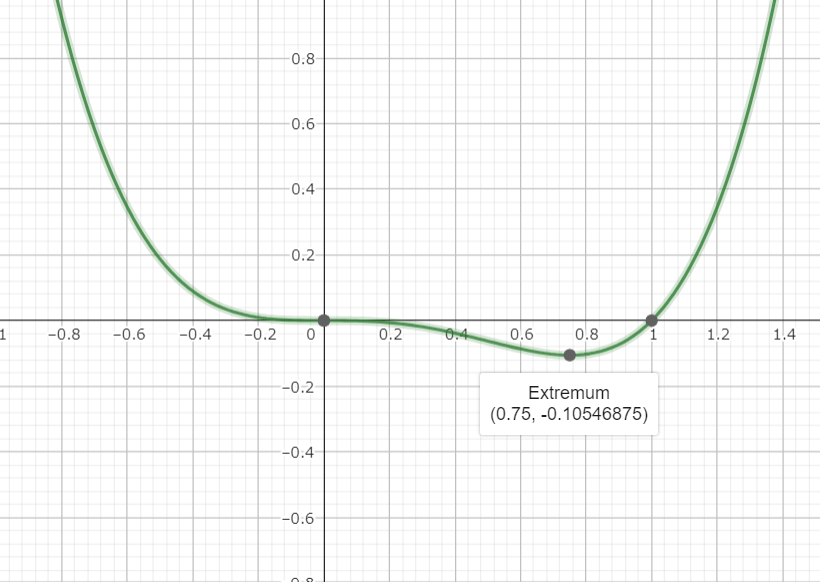
\includegraphics[scale=0.4]{img/QuuNote/x^4-x^3Graph.png}
                        \caption{$f(x)=x^4-x^3$のグラフ}\label{fig:x^4-x^3グラフ}
                    \end{figure}
                \clearpage
                \subsection{関数の変曲点}
                    さて、図\ref{fig:x^4-x^3グラフ}に着目すると$x=0$の前後で同じ単調減少でもすこし形が異なる様子が見られる。
                    $x<0$ではグラフの形が\textbf{下に凸}になっているが、$0<x<\frac{3}{4}$では\textbf{上に凸}になっている。
                    この違いは何なのだろうか。結論から述べるとこれは導関数の増減の変化から生じたものである。
                    例えば、$f'(x)$の導関数を求めると$f''(x)=12x^2-6x$であり$x=0$で$f''=0$である。つまり$x=0$で$f'(x)$の増減の仕方が変化した
                    わけである。$x<0$では$f''>0$なので$f'$は単調増加する、すなわち$f(x)$の減少の割合が小さくなっていくのである。これは下に凸にあたる。
                    一方$0<x(<\frac{1}{2})$では$f'$は単調減少する、つまり$f(x)$の減少の割合が大きくなっていくのである。これは上に凸にあたる。
                    ところで$f''$は$x=\frac{1}{2}$でも$0$になる。つまり$x>\frac{1}{2}$で$f''>0$なのでこのとき$f'$はまた単調増加し、$f(x)$の減少の割合が小さくなる。
                    これは上に凸に当たる。こうして減少の割合が小さくなっていき、$x=\frac{4}{3}$を超えると$f'>0$となる。いま$f'$は単調増加するわけだから、これ以降は$f(x)$
                    の増加の割合が大きくなっていくわけである。

                    以上をまとめると次の結果が得られる。
                    \begin{screen}
                        ある$x$の区間$I$について
                        \begin{itemize}
                            \item $f''(x)>0$である場合は$y=f(x)$は区間$I$で\underline{下に凸}
                            \item $f''(x)>0$である場合は$y=f(x)$は区間$I$で\underline{上に凸}
                        \end{itemize}
                        が成り立つ。ただし、$f(x)$が二階微分可能であるとする。
                    \end{screen}
                    ここで二階微分という言葉が出てきたが、これは単に二回微分できるという意味である。ここで
                    $f''=0$を満たす点$(x,y)$のことを\textbf{変曲点}という。名前から推察できるように下に凸・上に凸というのは
                    グラフの曲がり方のことを言っており、変曲点はその曲がり方が変わる点である。今回の場合は$(0,0),(\frac{1}{2},-\frac{1}{16})$である。これを用いればグラフの形をより正確に書くことができる。

                    では二階微分を用いて先ほどの表\ref{ta:f(x)=x^4-x^3の増減表}を書き直してみると、
                    \begin{table}[h]
                        \centering
                        \begin{tabular}{|c||c|c|c|c|c|c|c|}\hline
                            $x$ & $\cdots$ & $0$ & $\cdots$ & $\frac{1}{2}$ & $\cdots$ & $\frac{3}{4}$ & $\cdots$ \\\hline
                            $f'(x)$ & $-$ & $0$ & $-$ & $-$ & $-$ & $0$ & $+$ \\\hline
                            $f''(x)$ & $+$ & $0$ & $-$ & $0$ & $+$ & $+$ & $+$ \\\hline  
                            $f(x)$ & \ser  & $0$ & \sel & $-\frac{1}{16}$ & \ser &$-\frac{27}{256}$ & \ner \\\hline
                        \end{tabular}
                        \caption{$f(x)=x^4-x^3$の増減表(変曲点付き)}\label{ta:f(x)=x^4-x^3の増減表(変曲点付き)}
                    \end{table}

                    矢印を直線ではなく若干曲げることで上に凸・下に凸を表現した。
                \clearpage
                \subsection{関数の最大・最小}
                    さて、ここまでグラフについての応用を述べたが、それ以外にも関数の増減を調べることでわかることがある。
                    それは特定の区間内における$f(x)$の最大値・最小値である。具体的に言えばその区間内の極値と区間の端点の値とを
                    比べればよい。なぜなら、端点から極値までの値は単調に増加・減少するからである。そしてここから、$f(x)$が
                    極大値(極小値)を一つだけ持つなら、それが$f(x)$の最大値(最小値)であることもわかる。\\

                    関数の最大・最小がわかることは、関数の大小関係を比べる際に役立つ。例えば、$x\geq \sin x\quad(0\leq x < 2\pi)$
                    を示すとする。$f(x)=x-\sin x$とおいて微分すると$f'=1 - \cos x = 0$となる。$[0,2\pi)$の区間でこの方程式の解は$x=0$のみであり、
                    $x>0$で$f'>0$であるため、$[0,2\pi$)で$f$は単調増加である。すなわち$x=0$が$f$の最小値でありその値は$f(0)=0$となるため、$f(x)\geq 0$と
                    書ける。よって移項して$x\geq \sin x$だと示せた。
                    \begin{figure}[h]
                        \centering
                        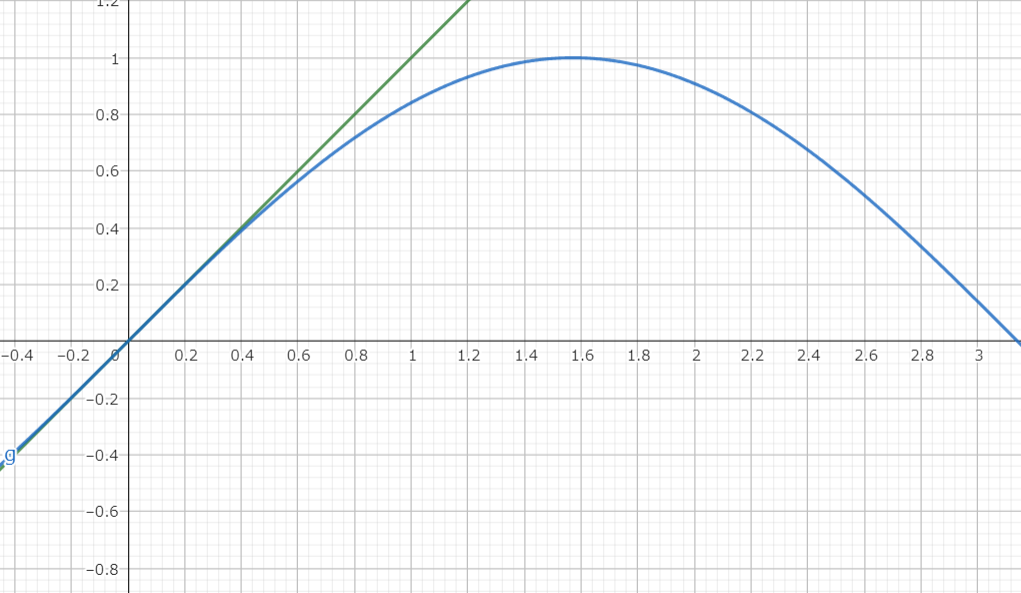
\includegraphics[scale=0.5]{img/QuuNote/x-sinxGraph.png}
                        \caption{$y=x,y=\sin x$のグラフ}
                    \end{figure}
                \clearpage
                \subsection{物理と微分}
                    この節の最後に物理と微分との関係について述べよう。力学では速度・加速度というものを学んだ。例えば速度は、「平均の速度」と「瞬間の速度」というものがあったと思う。
                    瞬間の速度の定義は
                    \begin{equation}
                        \frac{\Delta x}{\Delta t}
                    \end{equation}
                    であり、瞬間の速度は$\Delta t$を極めて小さくしていった場合の速度であった。この極めて小さく,というのは数学的には$\Delta t\to 0$の極限の操作をとることである。
                    つまり、瞬間の速度というのは平均の速度$\bar{v}$を$\Delta t\to 0$の極限値であり、これは変位$x(t)$の時間微分に等しい。
                    数式で書けば
                    \begin{equation}
                        v=\frac{dx}{dt}=\dot{x}(t)
                    \end{equation}
                    である。同様に、「瞬間の加速度」も
                    \begin{equation}
                        a=\frac{dv}{dt}=\frac{d^2 x}{dt^2}=\ddot{x}
                    \end{equation}
                    記号$d^2/dt^2$は二階微分を表す。このことから有名なニュートンの運動方程式も
                    \begin{equation}
                        F=m\ddot{x}
                    \end{equation}
                    という微分方程式になることがわかる。さて、ここからは少し背伸びしてベクトル解析の内容に入る。
                    というのも、変位や力など物理で出てくる量というのは大抵ベクトルが多いわけで、スカラー量の微分だけでは
                    応用例を紹介するのも難しいわけである。ベクトルの微分というと難しそうに聞こえるが、実は単純である。
                    ベクトルの関数$\bm{f}(t) =[f(t),g(t)]$\footnote{これをベクトル値関数という。}であるので、これを$t$で微分することは各成分を微分することであり、
                    $\dot{\bm{f}}=[f',g']$である。例えば運動方程式は
                    \begin{equation}
                        \bm{F}=m\ddot{\bm{x}}\label{eq:ニュートンの運動方程式}
                    \end{equation}
                    となる。また、位置ベクトルを$\bm{r}$とすると速度ベクトルは$\bm{v}=\dot{\bm{r}}$であり、加速度ベクトルは$\bm{a}=\ddot{\bm{r}}$である。
                    では、これを用いて等速円運動の速度ベクトルと加速度ベクトルを導いてみよう。簡単のため原点を中心とする円上の運動で、円の半径は$1$であり、$t=0$で座標は$(1,0)$とする。
                    このとき、位置ベクトルは$\bm{r}(t)=[\cos t,\sin t]$である。このとき、速度ベクトルは$\bm{v}=[-\sin t,\cos t]$であり、
                    加速度ベクトルは、$\bm{a}=[-\cos t,-\sin t]=-\bm{r}$となる。また、$\bm{r}\cdot \bm{v}=\bm{v}\cdot\bm{a}=0$である。
                    したがって、等速円運動では加速度ベクトルは常に円の中心を向き、位置ベクトルと速度ベクトル、速度ベクトルと加速度ベクトルはそれぞれ直行することがわかる。

                    さて、この結果を式\eqref{eq:ニュートンの運動方程式}に代入してみると、次のようになる。
                    \begin{equation}
                        \bm{F}=m\ddot{\bm{x}}=-m\bm{r}
                    \end{equation}
                    つまり、等速円運動では原点に向かって力が発生するのである。これを\textbf{向心力}という。一方、等速円運動する物体と
                    同じ座標系では加速度は0なわけだから、慣性の法則が成り立つように$m\ddot{\bm{r}}$という力を考え式を立てると$(-m\ddot{\bm{r}})+(m\ddot{\bm{r}})=m\cdot (0)$となる。
                    すなわち、等速円運動する座標系では向心力と逆向きの見かけ上の力が働いていることになる。これを\textbf{慣性力}といい、特に円運動の場合は\textbf{遠心力}という。
                    ちなみに等速円運動に限らず、物体の運動の加速度は接線方向の加速度ベクトルと法線方向のベクトルの加速度ベクトルの和として表せ、
                    これを運動方程式に代入した時の法線加速度の項が向心力になる。
                \clearpage
                \basicquestion 以下の問いに答えよ。

                \paragraph{問1}次の関数のグラフをかけ。\\
                $(1)y=x^3-x^2$\hspace{3mm}
                $\displaystyle(2)y=\frac{1}{1+x^2}$\hspace{3mm}
                $\displaystyle(3)y=e^{-x^2}$\hspace{3mm}
                $\displaystyle(4)y=\frac{\log x}{x}$

                \paragraph{問2}次の関数の(\hspace{1mm})内での最大・最小を求めよ。\\
                $(1)y=x^5-x^3+1\quad(-1\leq x\leq 1)$\hspace{3mm}
                $(2)e^x(x-1)\quad(-1\leq x\leq 2)$

                \paragraph{問3}$e^x \geq x+1 \quad (x\geq0)$を示せ。

                \paragraph{問4}図\ref{fig:直流回路}の直流回路について、最初に流れる電流$I$は以下の式で表される。
                \begin{equation*}
                    I=\frac{E}{R_0+R}\quad(\text{オームの法則})
                \end{equation*}
                また、可変抵抗器$R$で消費される電力$P$は$P=I^2R$である。この時、可変抵抗器で消費される最大の電力$P_{max}$
                の値を求めよ。また、この時の可変抵抗器の値を求めよ。

                \begin{figure}[h]
                    \centering
                    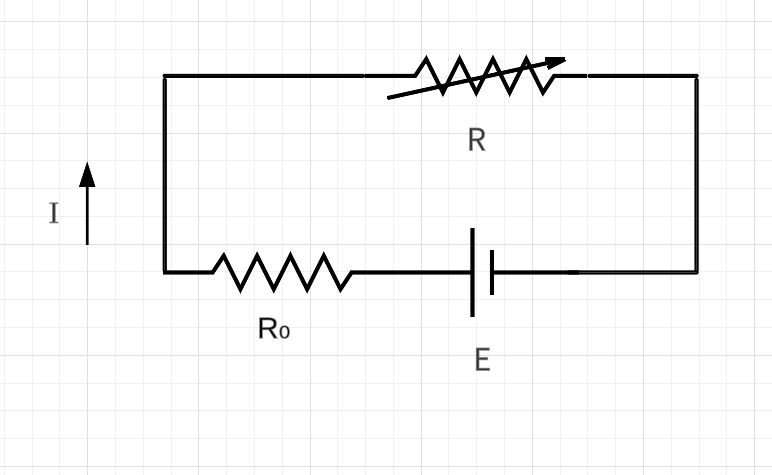
\includegraphics[scale=0.5]{img/QuuNote/tyokuryuukairo.png}
                    \caption{直流回路}\label{fig:直流回路}
                \end{figure}
            \clearpage
            \section{微分法諸定理}
                \subsection{$n$階微分とライプニッツの公式}
                    $y=f(x)$の導関数は$f'(x)$と表記される。では二階微分した場合はどうなるのかというと、これは変曲点の話ですでに出てきた通り$f''(x)$
                    である。これに準じて、三階微分、四階微分、...も$f'''(x),f''''(x),\cdots$と続く。しかしこれだと勝手が悪いので$'$の数だけ上に添え字で書くことが多い。
                    つまり、$f'''(x)=f^{(3)}(x),f''''(x)=f^{(4)}(x)$である。また、$n$階の導関数$f^{(n)}(x)$は$y^{(n)},D_x^{(n)} y,\displaystyle \frac{d^n y}{dx^n}$と書いたりもする。
                    これらは$n$次導関数ともいう。

                    \paragraph{例}$y=a^{x}$は$y'=a^x\log a,y''=a^x(\log a)^2,y^{(3)}=a^x(\log a)^3$である。一般に$y^{(n)}=a^x(\log a)^n$\\

                    さて、ここで積の$n$階微分について考えてみよう。\footnote{足し算・引き算は線形性より$(u\pm v)^{(n)}=u^{(n)}\pm v^{(n)}$がすぐわかってつまらない。かといって商の微分や合成関数の微分は計算が複雑すぎて
                    公式を導出するのも大変である。(なおかつその公式も複雑である。)}とりあえず、$n=1,2$のときで計算してみると
                    \begin{align*}
                        (uv)^{(1)}&=uv'+u'v\\
                        (uv)^{(2)}&=(uv'+u'v)^{(1)}=(uv')'+(u'v)'=u'v'+uv''+u''v+u'v'\\
                        &=u''v+2u'v'+uv''
                    \end{align*}
                    $n=1$のときは積の微分公式である。$n=2$は二項定理に形が似ている。$n=0$は微分していないことを意味するので、$u^{(2)}v^{(0)}+2u^{(1)}v^{(1)}+u^{(0)}v^{(2)}$
                    と書けばより二項定理っぽいことがわかる。実際$(u+v)^2=u^2v^0+2u^1v^1+u^0v^2$で形が一緒である。ちなみに$n=3$も$(uv)^{(3)}=u^{(3)}v+3u^{(2)}v^{(1)}+3u^{(1)}v^{(2)}+uv^{(3)}$
                    となって形が二項定理と一緒である。よって$n$階微分は次のような形になると予想される。
                    \begin{equation*}
                        (uv)^{(n)}={}_nC_0u^{(n)}v+{}_nC_1u^{(n-1)}v^{(1)}+{}_nC_2u^{(n-2)}v^{(2)}+\cdots + {}_nC_mu^{(n-m)}v^{(m)}+\cdots+{}_nC_nuv^{(n)}
                    \end{equation*}
                    ではこれを数学的帰納法を用いて証明しよう。まず$n=1$のときは明らかに成り立つ。一般に$n=i$のときまで成り立つと仮定すると$n=i+1$のときは
                    \begin{equation*}
                        (uv)^{(i+1)}=\left((uv)^{(i)}\right)'
                    \end{equation*}
                    となるので、
                    \begin{equation*}
                        \cdots + _iC_m(u^{(i-m)}v^{(m)})'+\cdots=\cdots_iC_{(m-1)}(u^{(i+2-m)}v^{(m-1)}+u^{(i+1-m)}v^{(m)}) + _iC_m(u^{(i+1-m)}v^{(m)}+u^{(i-m)}v^{(m+1)})+\cdots
                    \end{equation*}
                    式を整理して
                    \begin{equation*}
                        _iC_0u^{(i+1)}v+\left(_iC_0+_iC_1\right)u^{(i)}v^{(1)}+\cdots+\left(_iC_{(m-1)}+_iC_m\right)u^{(i+1-m)}v^{(m)}+\cdots+_iC_iuv^{(i+1)}
                    \end{equation*}
                    ここで、${}_iC_0={}_iC_i=1$であるため${}_iC_0=_{i+1}C_0,{}_iC_i={i+1}C_{i+1}$である。また、一般に${}_{i+1}C_m={}_iC_{m-1}+_iC_m$であるので、
                    \begin{equation*}
                        (uv)^{(i+1)}={}_{i+1}C_0u^{(i+1)}v+{}_{i+1}C_1u^{(i)}v^{(1)}+\cdots+{}_{i+1}C_{m}u^{(i+1-m)}v^{(m)}+\cdots+{}_{i+1}C_{i+1}uv^{(i+1)}                    
                    \end{equation*}
                    前述したように$n=1$のときは成り立つので、数学的帰納法より予想が正しいことが証明された。
                    \clearpage
                    したがって次の公式が得られる。
                    \begin{equation}
                        (uv)^{(n)}={}_nC_0u^{(n)}v+{}_nC_1u^{(n-1)}v^{(1)}+{}_nC_2u^{(n-2)}v^{(2)}+\cdots + {}_nC_mu^{(n-m)}v^{(m)}+\cdots+{}_nC_nuv^{(n)}\label{eq:ライプニッツの公式}
                    \end{equation}
                    これは\textbf{ライプニッツの公式}と呼ばれ、記号$\sum$を使って次のようにも書ける。
                    \begin{equation}
                        (uv)^{(n)}=\sum_{k=0}^{n} {_nC_k}u^{(n-k)}v^{(k)}
                    \end{equation}
                    こちらの方が簡潔に書ける。さらに、二項係数を$\dbinom{n}{k}$と書くことにすれば
                    \begin{equation}
                        (uv)^{(n)}=\sum_{k=0}^{n} \dbinom{n}{k}u^{(n-k)}v^{(k)}
                    \end{equation}
                    二項係数は$\binom{n}{k}$を使う教科書などのほうが多く、より一般的な書き方のようである。どちらの記号がよくてどちらがよくないかの判断は
                    こちらからは何とも言えないが、二項係数的な意味のときは$\binom{n}{k}$、組み合わせ論の話のときには$_nC_k$で使い分ければいいのではないだろうか。
                    これは好みのような気もする。
                \clearpage
                \subsection{ロルの定理}
                    ここではロルの定理について述べる。先に定理の内容についてあげておく。
                    \begin{itembox}{\textbf{ロルの定理}}
                        $[a,b]$で連続で$(a,b)$で微分可能な関数$f(x)$について、$f(a)=f(b)$ならば$f'(c)=0$となるような点$c\in(a,b)$が存在する。
                    \end{itembox}
                    これはグラフを書けば明らかである。$x$が$a\to b$に移動するとき、仮に$f(x)$が定数関数でなければ、
                    始めは$f(x)>f(a)$もしくは$f(x)<f(a)$になるはずである。しかし、$f(b)=f(a)$なので$x$が$b$に近くなるにつれて$f(a)$に近づかなければならない。
                    つまりどこかで増加から減少(もしくはその逆)になる点\footnote{これが極値であることはもう既知であろう。}が存在するはずなのである。$f(x)$が定数関数のときは明らかで$f'(x)=\frac{d}{dx}(\text{定数})=0$
                    である。

                    この定理は図を見ると意味がつかみやすい。区間を$[0,\pi]$でとっても$[-\pi,0]$でとっても$[-\pi,\pi]$でとっても良いが、
                    取った区間の間では必ず$f'(c)=0$となる$c$が存在しているのが一目でわかる。

                    \begin{figure}[h]
                        \centering
                        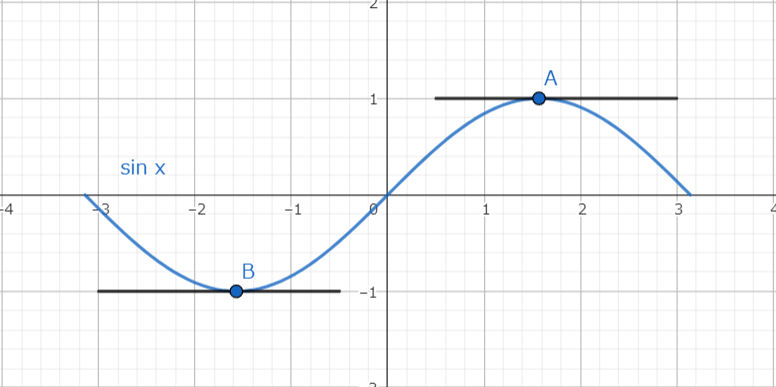
\includegraphics[scale=0.5]{img/QuuNote/rollTheory.png}
                        \caption{ロルの定理}
                    \end{figure}
                \clearpage
                \subsection{平均値の定理}
                    ここでは平均値の定理について述べる。こちらもロルの定理と同様に定理の内容からあげておく。
                    \begin{itembox}{\textbf{平均値の定理}}
                        $[a,b]$で連続で$(a,b)$で微分可能な関数$f(x)$について、
                        \begin{equation}
                            f'(c)=\frac{f(b)-f(a)}{b-a}\label{eq:平均値の定理}
                        \end{equation}
                        となるような点$c\in(a,b)$が存在する。
                    \end{itembox}
                    左辺は、$f(x)$の$(a,b)$上のある点での接線の傾きである。一方右辺は、以前述べた平均変化率の式そのままである。
                    すなわち平均値の定理は、点$(a,f(a)),(b,f(b))$を結んだ直線の傾きと接線の傾きが一致するような点が区間$(a,b)$に
                    少なくとも一つ存在することを示している。

                    それではお待ちかねの証明を示そう。まず、
                    \begin{equation*}
                        g(x)=\frac{f(b)-f(a)}{b-a}(x-a)+f(a)-f(x)
                    \end{equation*}
                    としておくことにする。このとき$g(x)$は$[a,b]$で連続で$(a,b)$で微分可能である。また$g(a)=g(b)=0$であることがわかる。
                    よってロルの定理が使えるので、$g'(c)=0$を満たす$c\in(a,b)$が存在するといえる。$g'(c)$を計算すると
                    \begin{equation*}
                        g'(c)=\frac{f(b)-f(a)}{b-a}-f'(c)=0
                    \end{equation*}
                    すなわち式\eqref{eq:平均値の定理}が成り立つ。$\square$

                    平均値の定理は様々な式の形に書き換えることができる。例えば
                    \begin{equation}
                        f(b)=f(a)+(b-a)f'(c)
                    \end{equation}
                    などはすぐ思いつくだろう。また、$a<c<b$なのだから$0<\theta<1$とすれば$c=a+\theta(b-a)$と書けるので
                    \begin{equation}
                        f(b)=f(a)+(b-a)f'(a+\theta(b-a))\quad(0<\theta<1)
                    \end{equation}
                    ともかける。またこれを微分係数のときと同じ要領で$h=b-a$と置けば
                    \begin{equation}
                        f(a+h)=f(a)+hf'(a+\theta h)\quad(0<\theta<1)\label{eq:平均値の定理1}
                    \end{equation}
                    とできる。さらに$a=x,h=\Delta x$と置けば
                    \begin{equation}
                        f(x+\Delta x)=f(x)+\Delta xf'(x+\theta\cdot\Delta x)\quad (0<\theta<1)\label{eq:平均値の定理x用}
                    \end{equation}
                    となる。もちろんこれらは式\eqref{eq:平均値の定理}を書き換えただけに過ぎないわけだが、目的によって
                    使い分けができるようになる。例えば、$\sqrt{5}$の近似値を平均値の定理で求めてみることにする。元の式からでは
                    どう求めるか見当もつかないが、式\eqref{eq:平均値の定理1}を用いれば$\sqrt{5}=\sqrt{4+1}$であるため、$f(x)=\sqrt{x}$と置けば
                    \begin{equation*}
                        f(4+1)=f(4)+f'(4+\theta)=2+\frac{1}{2\sqrt{4+\theta}}\thickapprox 2+\frac{1}{2\sqrt{4}}=2.25
                    \end{equation*}
                    として比較的自然に求められる。ちなみに$\sqrt{5}=2.23606\dots$であるので近似値の精度はそこまでよくない。
                \clearpage
                \subsection{コーシーの平均値の定理}
                    先ほど述べた平均値の定理を一般化してみよう。次の二つの関数$f,g$を考える。
                    この二つの関数は$[a,b]$で連続で、$(a,b)$で微分可能であるとする。またこの区間内では$g'\neq 0$であるとする。
                    この時平均値の定理から
                    \begin{equation*}
                        g(b)-g(a)=(b-a)g'(c_1)\quad(a<c_1<b)
                    \end{equation*}
                    $g'(c_1)$は仮定によって$0$ではないので、当然左辺も$0$ではない。そこで、
                    \begin{equation*}
                        \lambda=-\frac{f(b)-f(a)}{g(b)-g(a)}
                    \end{equation*}
                    とおき、関数
                    \begin{equation*}
                        F(x)=f(x)+\lambda g(x)
                    \end{equation*}
                    を作る。このとき、
                    \begin{align*}
                        F(a)&=f(a)+\lambda g(a)=\frac{f(a)(g(b)-g(a))-(f(b)-f(a))g(a)}{g(b)-g(a)}=\frac{f(a)g(b)-f(b)g(a)}{g(b)-g(a)}\\
                        &=\frac{(f(a)-f(b))g(b)+(g(b)-g(a)f(b))}{g(b)-g(a)}=f(b)+\lambda g(b)=F(b)
                    \end{align*}
                    であるので、ロルの定理が使えて、
                    \begin{equation*}
                        F'(c)=0\quad(a<c<b)
                    \end{equation*}
                    よって、
                    \begin{equation*}
                        F'(c)=f'(c)+\lambda g'(c)=0\leftrightarrow -\lambda = \frac{f'(c)}{g'(c)}
                    \end{equation*}
                    したがって次の\textbf{コーシーの平均値の定理}が得られる。
                    \begin{equation}
                        \frac{f(b)-f(a)}{g(b)-g(a)}=\frac{f'(c)}{g'(c)}\quad(a<c<b)\label{eq:コーシーの平均値の定理}
                    \end{equation}
                    ここで$g(x)=x$と置けば、平均値の定理\eqref{eq:平均値の定理}である。平均値の定理はコーシーの平均値の定理と区別して
                    ラグランジュの平均値の定理とも呼ばれる。
    
                \clearpage
                \subsection{ロピタルの定理}
                    極限値の計算を行っているときに、しばし
                    \begin{equation*}
                        \frac{0}{0},\quad\frac{\infty}{\infty},\quad\infty -\infty,\quad\infty\cdot\infty
                    \end{equation*}
                    などの\textbf{不定形}に遭遇するだろう。こういう不定形の極限値の計算で頭を抱えた経験も多いはずだ。不定形の解消には
                    様々な方法があるが、ここでは$0/0,\infty/\infty$の不定形に対して抜群な効果を発揮するロピタルの定理を示そう。
                    
                    例えば、$x\to a$の極限で$f(x)/g(x)\to 0/0$になってしまったとしよう。この時、$f'(x)/g'(x)$が極限値$b$に収束するならば、
                    $f(x)/g(x)$も同じ極限値$b$に収束する。なぜならコーシーの平均値の定理より、$f(a)=g(a)=0$のとき、$x>a$である$x$に対して
                    \begin{equation*}
                        \frac{f(x)}{g(x)}=\frac{f(x)-f(a)}{g(x)-g(a)}=\frac{f'(c)}{g'(c)}\quad(a<c<x)
                    \end{equation*}
                    ここで$x\to a$とすれば$c\to a$である。今$x>a$で考えているが、$x<a$の場合も同様なので、
                    \begin{equation}
                        \lim_{x\to a}\frac{f(x)}{g(x)}=\frac{f'(a)}{g'(a)}\label{ロピタルの定理}
                    \end{equation}
                    これを\textbf{ロピタルの定理}\footnote{ド・ロピタルの法則とも。}をいう。また、$f'(a)/g'(a)$が不定形$0/0$になるのなら
                    その時はもう一度ロピタルの定理を適用してあげて$f''(a)/g''(a)$と拡張できる。またロピタルの定理は$\infty/\infty$の不定形にも
                    適用できる。\footnote{証明は難しいので省略。$\varepsilon-\delta$論法を使えばできる。}

                    ロピタルの定理を用いて極限値を求めてみる。
                    \paragraph{例}
                        \begin{align*}
                            &(1) \lim_{x\to 0}\frac{\cos x-1}{x}=\lim_{x\to 0}\frac{-\sin x}{1}=0\\
                            &(2) \lim_{x\to \infty}\frac{e^{x}}{x}=\lim_{x\to\infty}\frac{e^x}{1}=\infty\\\
                            &(3) \lim_{x\to \infty}\frac{x^3+2x^2+1}{2x^3+1}=\lim_{x\to \infty}\frac{3x^2+4x}{6x^2}=\lim_{x\to\infty}\frac{6x+4}{12x}=\lim_{x\to\infty}\frac{6}{12}=\frac{1}{2}
                        \end{align*}
                        (1)は$0/0$、(2)は$\infty/\infty$の不定形である。また(3)はロピタルの定理を三回適用した場合である。
                    以下にロピタルの定理の間違った適用例を上げよう。
                    \begin{equation*}
                        \lim_{x\to 0}\frac{x}{\cos x}=\lim_{x\to 0}\frac{1}{-\sin x}=-\infty
                    \end{equation*}    
                    これは$0/0$の不定形でも$\infty/\infty$の不定形でもない。そもそも不定形ですらない。ロピタルの定理は使う前に条件をみたすかを確認しておきたいものである。
                    
                \clearpage
                \subsection{テイラーの定理}
                    最後に、テイラーの定理について述べよう。これはコーシーの平均値の定理とはまた違った平均値の定理\eqref{eq:平均値の定理}の一般化である。
                    先に定理について述べる。
                    \begin{itembox}{\textbf{テイラーの定理}}
                        関数$f(x)$が$[a,b]$で$n$階まで連続な導関数をもち、$(a,b)$で$n+1$階微分可能であるとき、ある点$c\in(a,b)$が存在し
                        \begin{equation}
                            f(b)=f(a)+f'(a)(b-a)+\frac{1}{2!}f''(a)(b-a)^2+\cdots+\frac{1}{n!}f^{(n)}(a)(b-a)^n+R_{n+1}\label{eq:テイラーの定理}
                        \end{equation}
                        ただし$R_{n+1}$は剰余項といい、
                        \begin{equation}
                            R_{n+1}=\frac{1}{(n+1)!}f^{(n+1)}(c)(b-a)^{n+1}\quad(a<c<b)
                        \end{equation}
                    \end{itembox}
                    $n=0$のときは平均値の定理\eqref{eq:平均値の定理}と同じである。証明は複雑であるが、平均値の定理と同様に証明できる。(証明は演習問題とする。)

                    平均値の定理のときと同様に、テイラーの定理から様々な表式を求めてみよう。平均値の定理と同様に$c=a+\theta(b-a)\quad(0<\theta<1)$と置く。
                    さらに$b=x$とすれば
                    \begin{alignat}{1}        
                        f(x)=&{}f(a)+f'(a)(x-a)+\frac{1}{2!}f''(a)(b-a)^2+\cdots+\frac{1}{n!}f^{(n)}(a)(x-a)^{n}\notag\\
                        &{}+\frac{1}{(n+1)!}f^{(n+1)}(a+\theta(x-a))(x-a)^{n+1}\label{eq:テイラー展開}
                    \end{alignat}
                    が得られる。これを関数$f(x)$の点$a$における\textbf{テイラー展開}という。さらに、テイラー展開の特別な場合として$a=0$を代入すれば
                    \begin{equation}
                        f(x)=f(0)+f'(0)x+\frac{1}{2!}f''(0)x^2+\cdots+\frac{1}{n!}f^{(n)}(0)x^n+\frac{1}{(n+1)!}f^{(n+1)}(\theta x)x^{n+1}\label{eq:マクローリン展開}
                    \end{equation}
                    これを関数$f(x)$の\textbf{マクローリン展開}という。テイラーの定理というとあまり馴染みのない言葉であるが、
                    テイラー展開/マクローリン展開と聞くと、理工学ではよく出てくるので知っている人も多いはずだ。
                    教科書などでは$R_{n+1}$を省略して$+\cdots$で終わっているものもあるかもしれないが、厳密に言えば間違いである。

                    \paragraph{マクローリン展開の例}$0<\theta<1$であるとする。
                        \begin{align}
                            e^x&=1+\frac{x}{1!}+\frac{x^2}{2!}+\cdots+\frac{x^n}{n!}+R_{n+1}\quad &&R_{n+1}=e^{\theta x}\frac{x^{n+1}}{(n+1)!}\label{eq:e^xのマクローリン展開}\\
                            \sin x &=x-\frac{x^3}{3!}+\frac{x^5}{5!}+\cdots+\frac{(-1)^{n-1}x^{2n-1}}{(2n-1)!}+R_{2n+1}\quad &&R_{2n+1}=\frac{(-1)^nx^{2n+1}}{(2n+1)!}\cos\theta x \label{eq:sin xのマクローリン展開}\\
                            \cos x &=1-\frac{x^2}{2!}+\frac{x^4}{4!}+\cdots+\frac{(-1)^{n}x^{2n}}{(2n)!}+R_{2n+2}\quad &&R_{2n+2}=\frac{(-1)^{n+1}x^{2n+2}}{(2n+2)!}\cos\theta x\label{eq:cos xのマクローリン展開}\\
                            \log(1+x) &= x-\frac{x^2}{2}+\frac{x^3}{3}+\cdots+(-1)^{n-1}\frac{x^n}{n}+R_{n+1}\quad &&R_{n+1}=\frac{(-1)^nx^{n+1}}{n+1}\left(\frac{1}{1+\theta x}\right)^{n+1}\label{eq:log(x+1)のマクローリン展開}
                        \end{align}
                    
                    さて、このような展開を用いれば関数$f(x)$を近似できるわけだが、より良く近似する際には項の数を増やし、$R_{n+1}$を
                    できるだけ小さくする必要があると予想できる。そこで、数列$\{R_n\}=R_1,R_2,R_3,\dots,R_n,\dots$を考え、数列$\{R_n\}$
                    が0に収束するときを考えてみよう。このとき
                    \begin{equation}
                        \lim_{n\to \infty}R_n=0
                    \end{equation}
                    であるので、より多くの項を取る($n\to\infty$)ほど、展開はよい近似になる。よって
                    \begin{equation}
                        f(x)=f(a)+f'(a)(x-a)+\cdots+f^{(n)}(a)\frac{(x-a)^n}{n!}+\cdots\label{eq:テイラー級数(テイラー展開)}
                    \end{equation}
                    と書く。最後の$\cdots$はどこまでも項を足していくことを意味する。この時\eqref{eq:テイラー級数(テイラー展開)}を\textbf{テイラー級数}という。
                    特に$a=0$なら、
                    \begin{equation}
                        f(x)=f(0)+f'(0)x+\cdots+f^{(n)}(0)\frac{x^n}{n!}+\cdots\label{eq:マクローリン級数(マクローリン展開)}
                    \end{equation}
                    となり、これを\textbf{マクローリン級数}と呼ぶ。

                    式\eqref{eq:テイラー級数(テイラー展開)}や式\eqref{eq:マクローリン級数(マクローリン展開)}は無限個の項を足し合わせており、このようなものを\textbf{無限級数}\footnote{加法はふつう有限のときに定義されるわけだから、無限個の和というのは形式的な表現である。実際の定義はのちに述べる。}という。
                    無限級数については第IV部で詳しく述べることにする。が面白い性質があるので先回りして紹介しておこう。
                    その性質とは、項別微分・項別積分ができることである。積分についてはまだ扱っていないので項別微分のみに着目しよう。これは名前の通り、項別に微分することができるということである。
                    例えば、$\sin x$のマクローリン級数は
                    \begin{equation}
                        \sin x=x-\frac{x^3}{3!}+\frac{x^5}{5!}+\cdots+\frac{(-1)^{n-1}x^{2n-1}}{(2n-1)!}+\cdots
                    \end{equation}
                    であり、左辺を微分すると$\cos x$である。一方右辺も項別に微分すると
                    \begin{equation}
                        \cos x = 1-\frac{x^2}{2!}+\frac{x^4}{4!}+\cdots+\frac{(-1)^{n-1}x^{2n-2}}{(2n-2)!}+\cdots
                    \end{equation}
                    となり$\cos x$のマクローリン級数\footnote{$2n-2=2(n-1)$なので$n'=n-1$と置けばきれいになる。}と一致する。この結果を用いれば$f(x)$の$n$次の微分係数を求めることなしに
                    マクローリン級数が求められることになる。
                \clearpage
                \basicquestion 以下の問いに答えよ。
                \paragraph{問1}次の関数の三次導関数を求めよ。\\
                $(1)y=(2x+1)^3$\hspace{3mm}
                $(2)\displaystyle y=\frac{1}{1+x}$\hspace{3mm}
                $(3)y=\sin(2x)$\hspace{3mm}
                $(4)y=xe^x$\hspace{3mm}
                $\displaystyle(5)y=\frac{\sin(2x)}{1+x}$

                \paragraph{問2}次の関数の$n$次導関数を求めよ。\\
                $(1)y=e^{-x}$\hspace{3mm}
                $(2)y=\cos x$\hspace{3mm}
                $(3)y=x^n$\hspace{3mm}
                $(4)y=\log(1+x)$

                \paragraph{問3}次の極限をロピタルの定理を用いて求めよ。\\
                $\displaystyle(1)\lim_{x\to 0}\frac{x-\log(1+x)}{x^2}$\hspace{3mm}
                $\displaystyle(2)\lim_{x\to 0}\frac{\sin^{-1}x}{x} $\hspace{3mm}
                $\displaystyle(3)\lim_{x\to \infty}\frac{\log x}{x}$\hspace{3mm}
                $\displaystyle(4)\lim_{x\to+0}x^x$\hspace{3mm}
                $\displaystyle(5)\lim_{x\to\infty}\log(1+e^x)^{\frac{1}{x}}$

                \paragraph{問4}次の極限をテイラー展開またはマクローリン展開を用いて求めよ。\\
                $\displaystyle(1)\lim_{x\to 0}\frac{x-\sin x}{x^3}$\hspace{50mm}
                $\displaystyle(2)\lim_{x\to \infty}\left\{\sqrt{x^2-3x+1}-x\right\}$

                \paragraph{問5}次の問いに答えよ。
                \begin{enumerate}\setcounter{enumi}{0}\renewcommand{\labelenumi}{(\arabic{enumi})}
                    \item $e^x$のマクローリン展開\eqref{eq:e^xのマクローリン展開}を示せ。
                    \item (1)の$x$に$ix$を代入せよ。
                    \item $\sin x$のマクローリン展開と$\cos x$のマクローリン展開と(2)から次の\textbf{オイラーの公式}\footnote{この公式は抜群に役に立つ。数学以外の様々な顔でも出し、特に$x=\pi$を代入した結果は人類の至宝とも称される。覚えておいて損はないと断言できる。}を導け。
                        \begin{equation}
                            e^{ix}=\cos x+i\sin x
                        \end{equation}
                \end{enumerate}
                
                \paragraph{問6}関数$f(x)$が$[a,b]$で$n$階まで連続な導関数を持ち、$(a,b)$で$n+1$階微分可能であるとする。また、次の二つをつくる。
                \begin{equation*}
                    g(x)=-f(b)+f(x)+f'(x)(b-x)+\frac{1}{2!}f''(x)(b-x)^2+\cdots+\frac{1}{n!}f^{(n)}(x)(b-x)^n+K(b-x)^{n+1}
                \end{equation*}
                \begin{equation*}
                    K=\frac{1}{(b-a)^{n+1}}\left[f(b)-\left\{f(a)+f'(a)(b-a)+\frac{1}{2!}f''(a)(b-a)^2+\cdots+\frac{1}{n!}f^{(n)}(a)(b-a)^n\right\}\right]
                \end{equation*}
                この時、テイラーの定理\eqref{eq:テイラーの定理}を証明せよ。
            \clearpage
            \section{第II部演習問題}
            \paragraph{問1}次の関数を微分せよ。\\
                $[1]y=x^3+x^2+x+1$\hspace{3mm}
                $[2]y=\cos^2 x-\sin^2 x$\hspace{3mm}
                $[3]y=\sinh(2x)$\hspace{3mm}
                $[4]y=\log\log\log x$\hspace{3mm}
                $[5]y=\log_{10}x$\\
                $[6]y=\cos(2\cos^{-1}x)$\hspace{3mm}
                $[7]y=\sin^{4}(3x)$\hspace{3mm}
                $\displaystyle[8]y=\frac{1}{\sqrt[3]{x^2+1}}$
            
            \paragraph{問2}次の関数のグラフをかけ。\\
                $[1]y=x^2e^x$\hspace{40mm}
                $[2]y=x^2\log x$\hspace{40mm}
                $[3]y=e^x\cos x$
            \paragraph{問3}次の極限を求めよ。\\
                $\displaystyle[1]\lim_{x\to 1}\frac{1+\cos\pi x}{(x-1)^2}$\hspace{10mm}
                $\displaystyle[2]\lim_{x\to 0}\frac{\sin x-x\cos x}{x^2\log(1+x)}$\hspace{10mm}
                $\displaystyle[3]\lim_{x\to\infty}\left\{\sqrt{(x+a)(x+b)}-\sqrt{(x-a)(x-b)}\right\}$
            \paragraph{問4}平均値の定理\eqref{eq:平均値の定理}を用いて$x>0$ならば$\sin x<x$を示せ。

            \paragraph{問5}次の問いに答えよ。
                \begin{enumerate}
                    \item $y=\tan^{-1}x$をマクローリン展開せよ。
                    \item 次を示せ。
                    \begin{equation*}
                        \frac{\pi}{4}=1-\frac{1}{3}+\frac{1}{5}-\cdots
                    \end{equation*}
                \end{enumerate}
            \paragraph{問6}次のマクローリン展開を証明し、これを用いて$\log 2$の値を小数点以下4位まで求めよ。
                \begin{equation*}
                    \log\left(\frac{1+x}{1-x}\right)=2\left(x+\frac{x^3}{3}+\frac{x^5}{5}+\cdots\right)
                \end{equation*}
            
            \paragraph{問7}$(1+x)^{\alpha}\quad(\alpha\text{は実数})$のマクローリン展開を求め、二項定理\eqref{eq:二項定理}を証明せよ。

            \paragraph{問8}以下の問いに答えよ。
                \begin{enumerate}\setcounter{enumi}{0}\renewcommand{\labelenumi}{(\arabic{enumi})}
                    \item $x,y$が変数$t$の関数として与えられているとき、$y$を$x$の関数(またはその逆)として考えられる。このとき、次の\textbf{媒介変数表示の微分公式}を導け。
                    \begin{equation}
                        \frac{dy}{dx}=\frac{\frac{dy}{dt}}{\frac{dx}{dt}}\label{eq:媒介変数の微分公式}
                    \end{equation}
                    \item 次の関数について$dy/dx$を求めよ。\\
                    $[1]x=\sin \theta,y=\cos\theta$\hspace{30mm}
                    $[2]x=t^3+2t,y=-t^2+3t$
                \end{enumerate}
            
            \paragraph{問9}次の関数の与えられた$x$の値に対応する点における接線の方程式を求めよ。\\
                $[1]y=x^3-3x^2\quad(x=3)$\hspace{10mm}
                $[2]y=\tan x\quad(x=0)$\hspace{10mm}
                $\displaystyle[3]y=\frac{\sin x}{x}\quad(x=\pi)$
            \paragraph{問10}$y=a^x$を$a$で微分せよ。

            \paragraph{問11}次の関数の導関数の$x=0$での連続性を調べよ。
                \begin{equation}
                    f(x)=\left\{\begin{array}{cc}
                        x^2\sin\frac{1}{x}&(x\neq 0)\\
                        0&(x=0)
                    \end{array}\right.
                \end{equation}
            \clearpage
            \paragraph{問12}1つの平面の両側に二点$A,B$が与えられているとする。
            動点$P$がこの平面の両側でそれぞれ一定の速さ$v_a,v_b$で運動するとき、$P$が
            $A$から$B$まで最短の時間で行くべき経路を求めよ。(解析概論より)
            \begin{figure}[h]
                \centering
                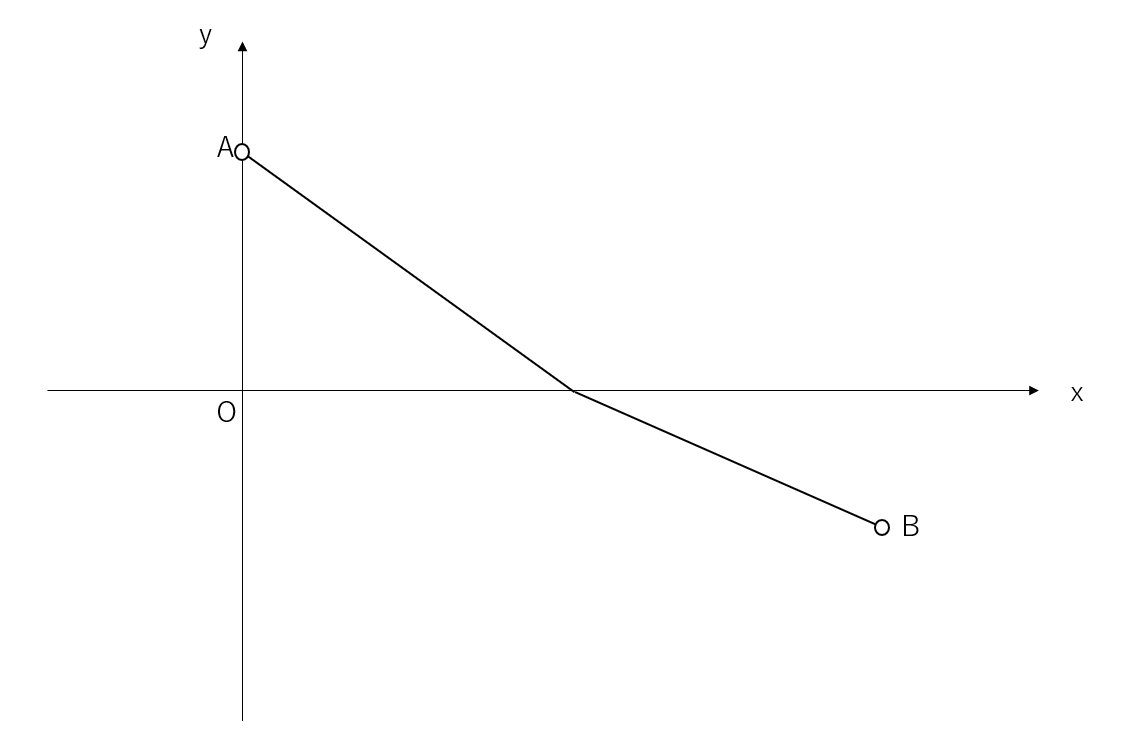
\includegraphics[scale=0.3]{img/QuuNote/snellQuestion.png}
                \caption{最短経路を求めよ}
            \end{figure}

            \paragraph{問13}次の\textbf{微分方程式}について以下の問いに答えよ。
                \begin{equation*}
                    y'-y^2-1=0
                \end{equation*}
                \begin{enumerate}\renewcommand{\labelenumi}{(\arabic{enumi})}
                    \item $y=\tan x$が方程式の解の一つであることを確かめよ。
                    \item (1)以外にどのような解が考えられるか。考えられる解を一つ答えよ。
                \end{enumerate}
            
            \paragraph{問14}指数関数$e^x$は$x$のどんな正のべきよりも早く増加し、対数関数$\log x$は
            $x$のどんな正のべきよりもゆっくり増加することを示せ。   
            
            \linktoMOKUZI
    \clearpage

    \part{積分$\int$}
        \vspace{\stretch{1}}
        \begin{screen}
            ついに微分積分の``積分''の話に移る。積分法は、微分方程式を解いたり、面積を求めたり...と様々な応用例がある。
            微分と違って具体的なイメージがしやすい反面、公式をそのまま適用できる場合が少なく、計算が難しい。
            微分と同じで慣れるまで問題をたくさん解くことで、ある程度感覚がつかめてくる。積分には定積分と不定積分の
            二つがあり、これらは互いに独立した概念である。順番としては不定積分,定積分,の順に扱う。
            歴史的には定積分,微分,不定積分の順に発明されたというのだから、面白い。なお、ここで扱うのはリーマン積分
            である。
        \end{screen}
        \clearpage
        \section{不定積分}
            \subsection{不定積分とは}
                これまで扱ってきた微分は現象の微小な変化を解析するものだった。しかし、現実には現象からある瞬間の変化を調べることに加えて、
                ある一瞬の変化から現象自身を得る必要も出てくる。実際の自然現象などは常に変化し続けており、それを定式化(方程式)にするには、
                ある瞬間の変化量を使うほうがその現象を本質的に見ることができる。例を示そう。例えば、空気抵抗を無視した
                物体の落下運動は最初の落下地点の高さをを$x_0$とすると$x(t)=-\frac{1}{2}gt^2+x_0$と表すことができる。
                しかし、変位の二階時間微分が加速度であることを考えれば$\ddot{x}=-g$と簡潔に表せる。
                これだけ見ると、別に微分を使って表す必要もなさそうである。では空気抵抗がある場合を考えてみよう。
                空気抵抗が速度に定数$k$で比例すると仮定すれば、微分を使わずに表すと\footnote{間違っているかも?各自で確認することをお勧めする。}
                \begin{equation}
                    x(t)=-\frac{m^2g}{k^2}e^{\frac{k}{m}t}+\frac{mg}{k}t+\frac{m^2g}{k^2}-\frac{mg}{k}+x_0
                \end{equation}
                のようになる。ちなみに$m$は質点の質量である。一方後者の方法で表すと
                \begin{equation}
                    m\ddot{x}=k\dot{x}-mg\label{eq:空気抵抗ありのときの落下運動}
                \end{equation}
                明らかに後者の方が簡単である。しかも後者の良いところは、初期条件($t=0$で$x=x_0$など)に関係なく同じ表式が得られるところで、
                これが現象の本質を表していることを示している。

                一方で、物理現象の本質を明らかにすることとは別に実際にその表式(今回の場合は変位)を得たい場合もある。
                その場合は式\eqref{eq:空気抵抗ありのときの落下運動}のような\textbf{微分方程式}では困るわけである。
                $y'=x$のような簡単な微分方程式なら$(x^2)'=2x$から簡単に解が予想できるが、$y'=x^2$や$y'=\sin 2x$など
                問題のたびに微分から予想していては大変である。また、式\eqref{eq:空気抵抗ありのときの落下運動}みたいに式が複雑になっていくと
                解の一つを予想するだけで苦労してしまう。そこで、微分と逆の演算である\textbf{積分}が登場する。この積分を学べば
                $y'(x)=f(x)$タイプの微分方程式はある程度統一的に解くことができるようになるのである。\\

                ここで、不定積分を(狭い範囲で)定義しよう。ある連続関数$f(x)$に対して
                \begin{equation}
                    F'(x)=f(x) \label{eq:原始関数定義}
                \end{equation}
                となる関数$F(x)$が存在した時、この関数$F(x)$を$f(x)$の原始関数、もしくは\textbf{不定積分}\footnote{実はこれは不定積分ではなく、原始関数の定義である。一般に原始関数と不定積分が等しくなる保証はないわけだが、
                $f$が連続関数であればこれらは同義になる。我々は今基本的に連続関数のみ扱いたいわけだから、これらを同じものとして扱っている。}という。
                この時$f(x)$を被積分関数といい、不定積分を次のように表す。
                \begin{equation}
                    F(x)=\int f(x)dx = \int dx f(x) \label{eq:不定積分の書き方}
                \end{equation}
                上のように$f(x)$と$dx$の順序はどちらでもよい。$f$があまりにも複雑なら最後に$dx$をつけ忘れてしまうかもしれない。その場合は後者の方がいい。
                一方多項式の間に積分が挟まれていて、どこからどこまでが$f$なのかがわかりにくいときなどは前者を使えばいい。

                ある関数の不定積分が$F(x)$なら、当然それに定数を加えた$F(x)+C$も$f$の不定積分になる。なぜなら
                \begin{equation*}
                    (F(x)+C)'=F'(x)+(C)'=F'(x)=f(x)
                \end{equation*}
                となるから当然である。つまり不定積分は定数の分だけ``不定''なのである。このような任意定数を積分定数という。
                
                また、定義から明らかに
                \begin{equation}
                    \int \frac{df}{dx}dx = f(x)+C
                \end{equation}
                であることがわかる。もちろん常にこんな簡単な積分ばかりではない。

                \paragraph{例}$\displaystyle\int x dx$を求める。$(x^2)'=2x$だから$x=\frac{1}{2}(x^2)'$
                \begin{equation*}
                    \int x dx = \int \frac{1}{2}(x^2)'dx=\frac{1}{2}\int (x^2)'dx=\frac{1}{2}x^2+C\quad (\text{$C$は積分定数})
                \end{equation*}

                上記の例のように、不定積分は微分演算の逆演算である。このことを利用して次節で様々な公式を導出する。
            \clearpage
            \subsection{不定積分の公式}
                ここでは不定積分の性質と公式についてまとめる。以下積分定数を省略する。まずは加法性について。
                \begin{equation}
                    \int \left\{f(x)\pm g(x)\right\}dx=\int f(x)dx\pm \int g(x)dx \label{eq:不定積分の加法性}
                \end{equation}
                である。これは定義からわかる。$f,g$の不定積分を$F(x),G(x)$と表すことにすれば
                \begin{equation}
                    (F(x)\pm G(x))'=(F(x))'\pm(G(x))'
                \end{equation}
                だから、これを両辺不定積分すれば
                \begin{equation}
                    F(x)\pm G(x)=\int \left\{(F(x))'+(G(x))'\right\}dx=\int \left\{f(x)\pm g(x)\right\}dx
                \end{equation}
                となり式\eqref{eq:不定積分の加法性}を得る。

                次に$f(ax+b)$について考えて見る。これも定義から$(F(ax+b))'=\frac{1}{a}F'(ax+b)$なのだから
                \begin{equation}
                    \int f(ax+b)dx=\frac{1}{a}F(ax+b)\label{eq:f(ax+b)の不定積分}
                \end{equation}

                では、それぞれの関数の不定積分を見ていこう。まずは$x^n$について考える。$n\neq -1$のとき
                $x^{n+1}$を微分すると、$(n+1)x^{n}$となるから次の公式が得られる。
                \begin{equation}
                    \int x^n dx = \frac{1}{n+1} x^{n+1}\quad (n\neq -1) \label{eq:x^nの不定積分}
                \end{equation}
                また、$n=-1$のときは$(\log |x|)'=\frac{1}{x}$であるため、
                \begin{equation}
                    \int \frac{dx}{x} = \log |x| \label{eq:1/xの不定積分} 
                \end{equation}

                三角関数については、$(\sin x)'=\cos x,(\cos x)'=-\sin x$であるから
                \begin{equation}
                    \int \sin xdx = -\cos x,\quad \int \cos x dx = \sin x \label{eq:sin,cosの積分}
                \end{equation}
                $\tan x$についても、$(\tan x)'=\frac{1}{\cos ^2x}$であるため
                \begin{equation}
                    \int \frac{1}{\cos^2 x}dx=\tan x \label{eq:tanの不定積分}
                \end{equation}

                指数関数$e^x$についてはどうだろうか。$(e^x)'=e^x$であるから
                \begin{equation}
                    \int e^x dx = e^x \label{eq:expの不定積分}
                \end{equation}
                である。一般の指数関数$a^x$は$(a^x)'=a^x \log a$より
                \begin{equation}
                    \int a^x dx =\frac{a^x}{\log a} \label{eq:a^xの不定積分}
                \end{equation}
                一方対数関数$\log x$の不定積分を求めるには、あるテクニック/公式が必要なのでここでは省略する。\\

                以上で述べたことは、原理を理解するのはもちろん公式として暗記しておくことを勧める。

            \clearpage
            \subsection{置換積分法}
                前節では、単純な関数の積分について述べた。しかし、これらの公式だけではほとんどの積分には太刀打ちできない。例えば
                \begin{equation*}
                    \int x(x^2+1)^{1000}dx
                \end{equation*}
                など、理論上は展開して計算できるが1000乗の展開など想像するだけでぞっとする。また、
                \begin{equation*}
                    \int x\sin(x^2)dx
                \end{equation*}
                などのような複雑な関数の積分はどのようの解けばよいだろうか。

                そこで、このような複雑な積分を計算する方法として\textbf{置換積分}法を紹介する。
                \begin{itembox}{置換積分の公式}
                    関数$\phi(t)$について$x=\phi(t)$と置くとき
                    \begin{equation}
                        \int f(x)dx = \int f(\phi(t))\phi'(t)dt \label{eq:置換積分}
                    \end{equation}
                    が成り立つ。
                \end{itembox}
                \paragraph{証明} 合成関数の微分法によって
                \begin{equation}
                    \frac{d}{dt}F(\phi(t))=F'(\phi(t))\phi'(t)=f(\phi(t))\phi'(t) 
                \end{equation}
                また、$x=\phi(t)$より
                \begin{equation}
                    \frac{d}{dx}F(\phi(t))=\frac{d}{dx}F(x)=f(x)
                \end{equation}
                よってそれぞれ$x,t$で不定積分すれば式\eqref{eq:置換積分}が得られる。\\

                \paragraph{例1}
                \begin{equation*}
                    \int x\sin(x^2)dx
                \end{equation*}
                を求める。$t=g(x)=x^2$と置くと、$g'(x)=2x$であるため、
                \begin{equation*}
                    \int \frac{1}{2}\sin(g(x))g'(x)dx=\int \frac{1}{2}\sin t dt = -\frac{1}{2}\cos t = -\frac{1}{2}\cos x^2
                \end{equation*}\\

                式\eqref{eq:置換積分}の$\phi'(t)$は$\frac{dx}{dt}$のことであるため、書き直すと
                \begin{equation}
                    \int f(\phi(t))\frac{dx}{dt}dt =\int f(x)dx 
                \end{equation}
                となり、あたかも$\frac{dx}{dt}$が$dt$で約分されているように見える。また、$t=g(x)$と置いて$\frac{dt}{dx}$を求める行為は
                形式的には両辺をそれぞれの文字$t,x$で微分して$dt,dx$を付けたものと等しくなる。つまり、$dt=g'(x)dx$を代入したように見える。
                この書き方は便利なのでしばし用いられるが、あくまで形式的なものに過ぎない。
                \clearpage
                \paragraph{例2}
                \begin{equation*}
                    \int \frac{dx}{\sqrt{1+x^2}}
                \end{equation*}
                を求める。$x=\sinh t$と置換すると$dx = \cosh t dt$であるため
                \begin{equation*}
                    \int \frac{\cosh t}{\sqrt{1+(\sinh t)^2}}dt=\int \frac{\cosh t}{\cosh t}dt=\int dt = t = \sinh^{-1} x
                \end{equation*}
                もちろんこのままでもいいが、いい機会なので$\sinh^{-1}x$の具体的な式を求めてみよう。まず、$\sinh$の定義より
                \begin{equation*}
                    x = \sinh t = \frac{e^t-e^{-t}}{2}=\frac{e^{2t}-1}{2e^t}
                \end{equation*}
                よって、両辺に$e^t$をかけて、$e^t$に関する二次方程式を解くと
                \begin{equation*}
                    e^{t} = \frac{2x\pm \sqrt{4x^2+4}}{2}=x\pm\sqrt{x^2+1}
                \end{equation*}
                $e^t>0$より、符号は$+$のみである。したがって、対数を取ると
                \begin{equation}
                    t=\sinh^{-1}x=\log\left(x+\sqrt{x^2+1}\right)\label{eq:arcsinh}
                \end{equation}\\

                さて、例3では式\eqref{eq:置換積分}の右辺から左辺への変形であった。置換積分は$x=\dots$と置く場合と
                $t=\dots$と置く場合とがある。どちらの場合でも対応できるようにしておきたいものである。ちなみに、いままで置換の変数に
                $t$を用いてきたが、こだわらなくてよい。つまり$u=x^2$と置いたり$x=\cos\theta$と置いても何も差し支えない。
            \clearpage
            \subsection{部分積分法}
                置換積分は合成関数の微分から導出されたものであるが、同じように積の微分から新たな公式を導出することができる。それが\textbf{部分積分法}
                であり、置換積分では計算できない積分などに使う。
                \begin{itembox}{部分積分法}
                    関数$f(x),g(x)$について
                    \begin{equation}
                        \int f(x)g'(x) dx = f(x)g(x) - \int f'(x)g(x)dx \label{eq:部分積分法}
                    \end{equation}
                    が成り立つ。
                \end{itembox}
                \paragraph{証明}積の微分公式より
                \begin{equation}
                    (fg)'=f'g+fg' \leftrightarrow fg' = (fg)'-f'g
                \end{equation}
                あとは両辺を積分すれば式\eqref{eq:部分積分法}が得られる。

                \paragraph{例1}
                \begin{equation*}
                    \int x\sin x dx
                \end{equation*}
                を求める。$f(x)=x,g'(x)=\sin x$とすると
                \begin{equation*}
                    \int x(-\cos x)'dx = -x\cos x + \int \cos xdx = -x\cos x+\sin x
                \end{equation*}
                となる。

                例1で、$f,g$をうまく選ばないと悲惨な結果になる。例えば$f=\sin x,g=x$と選ぶと
                \begin{equation*}
                    \int x\sin xdx=\frac{1}{2}x^2\sin x - \int \frac{1}{2}x^2\cos xdx
                \end{equation*}
                とまあより複雑な積分になってしまう。

                \paragraph{例2}$\log x$の不定積分を求める。$(x)'=1$より
                \begin{equation*}
                    \int \log xdx=\int (x)'\log xdx=x\log x - \int x\cdot \frac{1}{x}dx=x\log x-\int dx=x\log x-x
                \end{equation*}
                したがって次の公式が得られた。
                \begin{equation}
                    \int \log xdx=x\log x-x\label{eq:log xの不定積分}
                \end{equation}\\

                部分積分は、$fg$のうちすくなくとも片方の関数が微分したら周期的に元に戻る関数であるときによく使われる印象である。\footnote{例えば、$\sin x$は4回微分したら元の関数に戻る。$e^x$は1回である。}
                また、積分漸化式の問題でも用いられる。
            \clearpage
            \subsection{有理関数の不定積分}
                有理関数$R(x)$の不定積分については次の重要な性質がある。
                \begin{screen}\centering
                    有理関数$R(x)$は\underbar{必ず不定積分できる}。
                \end{screen}
                ここでいう``不定積分できる''とは、その関数の不定積分が初等関数の範囲で表せられることを言う。\footnote{一般に、初等関数の原始関数が初等関数になる\underbar{ことは起こりえない}。$e^{-x^2},\sin x/x$などが有名な例である。}
                今からこれを示すが、この証明を理解することよりも有理関数の不定積分ができることを覚えておくことのほうが重要である。\\

                さて、有理関数において分母の次数より分子の次数が高いとき、それは多項式と分母の次数のほうが高い有理関数の和で表すことができる。これには正式の除算を用いればよい。
                例えば、$\frac{x^3+2}{x+1}=x^2-x+1+\frac{1}{x+1}$
                
                多項式の積分の方が積分できるのはすぐわかるので、注目すべきは有理関数のほうである。この時この有理関数は
                \begin{equation}
                    \frac{1}{(ax+b)^n}\text{と}\frac{px+q}{\left\{(x-a)^2+b^2\right\}^n}
                \end{equation}
                の和の形に必ず分解することができる。\footnote{参考:\url{https://www.math.titech.ac.jp/~hoya/Teaching/calculusI2023PDF/bubunbunsu.pdf}}
                
                まず前者の積分であるが、これは簡単である。公式を用いて
                \begin{equation}
                    \int \frac{dx}{(ax+b)^n} = \left\{\begin{array}{lc}
                        \displaystyle \frac{1}{a(-n+1)}\frac{1}{(ax+b)^{n-1}} & (n\neq 1) \\
                        \displaystyle \frac{1}{a}\log|ax+b| & (n=1)
                    \end{array}\right.
                \end{equation}
                となる。後者は少し難しい。式を変形すると
                \begin{equation*}
                    \frac{px+q}{\left\{(x-a)^2+b^2\right\}^n}=\frac{p}{2}\frac{2(x-a)}{\left\{(x-a)^2+b^2\right\}^n}+\frac{(q+pa)}{\left\{(x-a)^2+b^2\right\}^n}
                \end{equation*}
                と分けられる。右辺第一項の積分は、$t=(x-a)^2+b^2$の置換を行うと
                \begin{equation*}
                    \frac{p}{2}\int \frac{dt}{t^n}=\frac{p}{2(-n+1)}\frac{1}{t^{n-1}}=\frac{p}{2(-n+1)}\frac{1}{\left\{(x-a)^2+b^2\right\}^{n-1}}
                \end{equation*}
                となる。問題は二項目の積分であり、これを直接解こうとすると大変である。ここは、積分を$I_n$と置いて$n$についての漸化式を作る。定数部分は関係ないので省略する。
                \begin{align*}
                    I_n &= \int \frac{dx}{\left\{(x-a)^2+b^2\right\}^n}=\int \frac{dt}{(t^2+b^2)^n} = \frac{t}{(t^2+b^2)^n} - \int (-2n)\cdot\frac{t^2}{(t^2+b^2)^{n+1}}dt\\
                        &= \frac{t}{(t^2+b^2)^n}+2n\int \frac{t^2+b^2-b^2}{(t^2+b^2)^{n+1}}dt=\frac{t}{(t^2+b^2)^n}+2nI_n-2nb^2I_{n+1}
                \end{align*}
                $n+1=m$と置き、式を整理すると、
                \begin{equation}
                    I_m = \frac{1}{b^2}\left[\frac{2m-3}{2m-2}I_{m-1}+\frac{1}{2(m-1)}\frac{(x-a)}{\left\{(x-a)^2+b^2\right\}^{m-1}}\right] \label{eq:有理関数の不定積分漸化式}
                \end{equation}
                \clearpage
                式\eqref{eq:有理関数の不定積分漸化式}から、$I_m$を求めるには$I_{m-1}$を、$I_{m-1}$を求めるには$I_{m-2}$を・・・とどんどん遡っていき$m=2$まで行くと、不定積分は求められる。
                なぜなら$m=2$つまり$n=1$のとき
                \begin{equation*}
                    I_1 = \int \frac{dx}{(x-a)^2+b^2}=\frac{1}{b}\tan^{-1}\left(\frac{x-a}{b}\right) 
                \end{equation*}
                となるからである。以上の結果から有理関数の不定積分は\underline{常に求められる}。\\

                とはいえ、有理関数の不定積分を求めることは簡単なことではなく、計算は煩雑になりがちである。
                大事なのは、冒頭でも述べた通り不定積分できるという認識を持っておくことである。

                \paragraph{例1}
                \begin{equation*}
                    \int \frac{dx}{x^2-1}
                \end{equation*}
                を求める。分母を因数分解すると$x^2-1=(x-1)(x+1)$であるため、
                \begin{equation*}
                    \frac{1}{x^2-1}=\frac{1}{(x-1)(x+1)}=\frac{1}{2}\left(\frac{1}{x-1}-\frac{1}{x+1}\right)
                \end{equation*}
                と部分分数分解して
                \begin{equation*}
                    \int \frac{dx}{x^2-1}=\frac{1}{2}\left(\int \frac{dx}{x-1}-\int \frac{dx}{x+1}\right)=\frac{1}{2}\left(\log|x-1|-\log|x+1|\right)=\frac{1}{2}\log\left|\frac{x-1}{x+1}\right|
                \end{equation*}

                上の例では部分分数分解が簡単にできるが、中には部分分数分解すること自体が大変な場合もある。
                \paragraph{例2}
                \begin{equation*}
                    \frac{1}{x^3+1}
                \end{equation*}
                を部分分数分解する。分母を因数分解すると$x^3+1=(x+1)(x^2-x+1)$より
                \begin{equation*}
                    \frac{1}{x^3+1}=\frac{1}{(x+1)(x^2-x+1)}=\frac{A}{x+1}+\frac{Bx+C}{x^2-x+1}
                \end{equation*}
                と置いて\footnote{二項目は分母が二次式なので分子は$(n-1)=1$次式で置く。}、この恒等式から$A,B,C$を求めればよい。\footnote{$1/(x^2-1)$のときも同様に求めてよい。ただこの場合は簡単なので省いただけ。}
                両辺の分母に$(x+1)(x^2-x+1)$を掛けると
                \begin{equation*}
                    1 = A(x^2-x+1)+(Bx+C)(x+1)=(A+B)x^2+(-A+B+C)x+(A+C)
                \end{equation*}
                となるため、
                \begin{equation*}
                    \left\{\begin{array}{rrccccl}
                        &A&+&B& &&=0\\
                        -&A&+&B&+&C & = 0\\
                        &A&&&+&C &=1
                    \end{array}\right.
                \end{equation*}
                の連立方程式を解く。あとは代数の計算なので普通に解けばよい。係数的にクラメルの公式が簡単である。
                $(A,B,C)=(\frac{1}{3},-\frac{1}{3},\frac{2}{3})$より
                \begin{equation*}
                    \frac{1}{x^3+1}=\frac{1}{3}\left(\frac{1}{x+1}+\frac{-x+2}{x^2-x+1}\right)
                \end{equation*}

            \clearpage
            \basicquestion 以下の問いに答えよ。積分定数は省略してもよい。

            \paragraph{問1}次の不定積分を求めよ。\\
                $(1)\displaystyle \int x^3dx$\hspace{3mm}
                $(2)\displaystyle \int \sin(-x) dx$\hspace{3mm}
                $(3)\displaystyle \int \left(e^{2x}+\frac{1}{x^2}\right)dx$\hspace{3mm}
                $(4)\displaystyle \int \frac{dx}{ex}$\hspace{3mm}
                $(5)\displaystyle \int \left(\tan^2 x + 1\right)dx$\hspace{3mm}
                $(6)\displaystyle \int \sin x\cos xdx$\\

            \paragraph{問2}次の不定積分を(\hspace{1mm})内の置換によって求めよ。\\
                $(1)\displaystyle \int x\cos(x^2)dx \quad (t=x^2)$\hspace{3mm}
                $(2)\displaystyle \int x^2(x^3-1)^2dx\quad (t=x^3-1)$\hspace{3mm}
                $(3)\displaystyle \int \frac{dx}{x^2+1}\quad (x=\tan \theta)$\\
                $(4)\displaystyle \int \frac{dx}{\sqrt{1-x^2}}\quad (x=\sin \theta)$\hspace{3mm}
                $(5)\displaystyle \int \sin^3 x\cos x dx \quad(t=\sin x)$\\
            
            \paragraph{問3}次の不定積分を部分積分法で求めよ。{\scriptsize (3)ヒント:$I=$と置き、二回部分積分せよ。}\\
                $(1)\displaystyle \int x\cos xdx$\hspace{3mm}
                $(2)\displaystyle \int xe^x dx$\hspace{3mm}
                $(3)\displaystyle \int e^x\cos xdx$\hspace{3mm}
                $(4)\displaystyle \int \log(x^2+1)dx$\hspace{3mm}
                $(5)\displaystyle \int \sqrt{a^2-x^2}dx$

            \paragraph{問4}次の不定積分を部分分数分解を用いて求めよ。\\
                $(1)\displaystyle \int \frac{dx}{x^2-3x+2}$\hspace{20mm}
                $(2)\displaystyle \int \frac{dx}{(x^2+1)(x-2)}$\hspace{20mm}
                $(3)\displaystyle \int \frac{dx}{x^2-a^2}\quad (a>0)$\\

            \paragraph{問5}以下証明せよ。
                \begin{enumerate}\setcounter{enumi}{0}\renewcommand{\labelenumi}{(\arabic{enumi})}
                    \item $\displaystyle \int \sinh x dx = \cosh x$を示せ。
                    \item $\sin x,\cos x$の有理関数を$f(\sin x,\cos x)$と表す\footnote{例えば、$\frac{\sin x}{1+\cos x}$は、$f(X,Y)=\frac{X}{1+Y}$の形である。引数が二つあると二変数関数みたいに見えるが実際には$x$だけの関数である。}
                    とする。このとき不定積分
                        \begin{equation*}
                            \int f(\sin x,\cos x)dx
                        \end{equation*}
                        は$t=\tan\frac{x}{2}$の置換により必ず積分できることを示せ。
                \end{enumerate}
        \clearpage
        \section{定積分}
            \subsection{面積を求めるには}
                不定積分の話はいったん忘れて、一度素朴な話題に移ろう。古来より様々な図形の面積が求められた。
                もっとも有名で美しい図形でよく上げられるのは円である。図形の面積の求め方には大きく二つある。この二つの方法で円の面積を求めてみることにしよう。

                まず、最初に思いつく方法としては\textbf{取りつくし法}だろう。これはすでに面積が既知である図形(例えば長方形)などの図形で、円を
                埋め尽くして面積を求める方法で、やり方は至極簡単である。
                \begin{figure}[h]
                    \centering
                    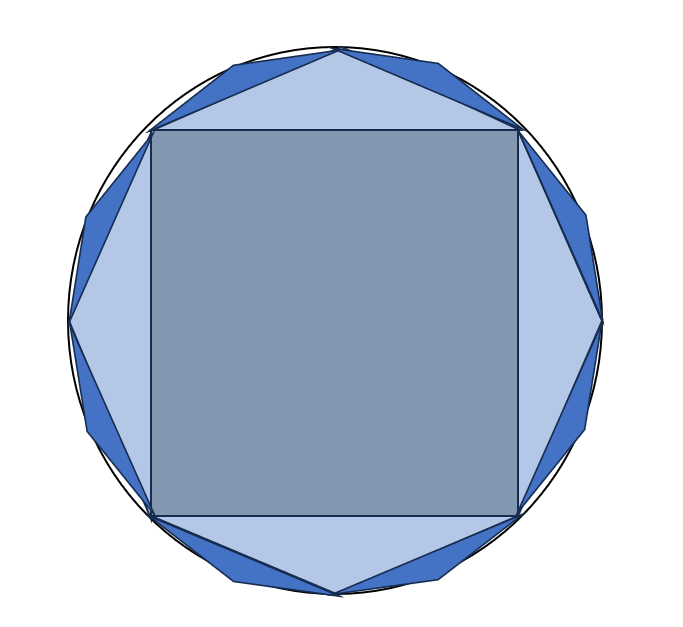
\includegraphics[scale=0.35]{img/QuuNote/Tritukusi.png}
                    \caption{取りつくし法による円の面積}
                \end{figure}

                ただ、取りつくし法の問題点は一般性がないことである。例えば上記の例では正方形と二種類の二等辺三角形で円の面積を近似しているが、
                正$n$角形で近似する方法もある。しかし、対象の図形が楕円などで異なった場合は、その図形に応じて取りつくしの方法も変わってしまう。

                そこで古代から考えられてきたもう一つの方法として\textbf{区分求積法}がある。
                これは図形を短冊状の図形に区切ってそれぞれの面積を面積を求め、それらを足す方法である。
                \begin{figure}[h]
                    \centering
                    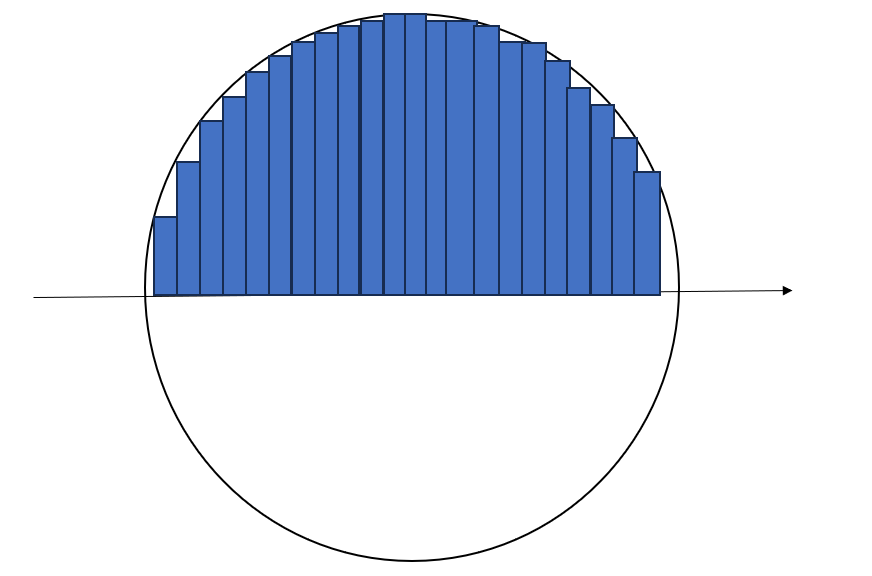
\includegraphics[scale=0.35]{img/QuuNote/kubunkyuseki.png}
                    \caption{区分求積法による半円の面積}
                \end{figure}

                これの良いところは。図形の形によらず同じ方法で図形の面積が求められることである。そのため図形の上部を
                を適当な関数で表せればよいことになる。区分求積法も古来より用いられてきた方法であるが、実際に面積を求めるのは
                簡単なことではない。そこで、\textbf{定積分}が登場する。
            \clearpage
            \subsection{定積分の定義}
                以下に定積分の定義を述べよう。まず、xy平面上の関数$y=f(x)$の区間$[a,b]$での面積を求めることを考える。簡単にするために、$[a,b]$で$f\geq0$であるとする。
                $[a,b]$の間に$x_0=a,x_1,x_2,\dots,x_n=b$の$n+1$個の点を考え、$z_k \in [x_{k-1},x_{k}]$である任意の点$z_1,z_2,z_3,\dots,z_{n}$を考える。
                $\Delta x_k=x_{k}-x_{k-1}$と定義すると、$y=f(x)$と直線$x=a,x=b$とx軸で囲まれた面積$S$の近似値$S_{\Delta}$は次のように与えられることがわかる。
                \begin{equation}
                    S_{\Delta} = \sum_{k=1}^{n}f(z_k)\Delta x_{k} \label{eq:リーマン和の定義}
                \end{equation}
                式\eqref{eq:リーマン和の定義}で定義された量$S_{\Delta}$を\textbf{リーマン和}\footnote{本によっては積和と呼ぶこともある。このノート中はどちらとも使っているかもしれない。}と呼ぶ。この積和に$n\to \infty$の極限を取る\footnote{高専の教科書では$\Delta x_k \to 0$としているが、このノートでは解析概論等の数学書に合わせ$n\to 0$とする。どちらも本質は同じである。}、つまり
                分割の数を極限まで大きくして、ある一定の値に収束したとき、これを
                \begin{equation}
                    \int_a^b f(x)dx = \lim_{n\to\infty}\sum_{k=1}^{n}f(z_k)\Delta x_k \label{eq:定積分の定義}
                \end{equation}
                と表す。この左辺を$y=f(x)$の区間$[a,b]$での\textbf{定積分}といい、この値は$S$に等しい。(下図\eqref{fig:定積分図}参照)

                \begin{figure}[h]
                    \centering
                    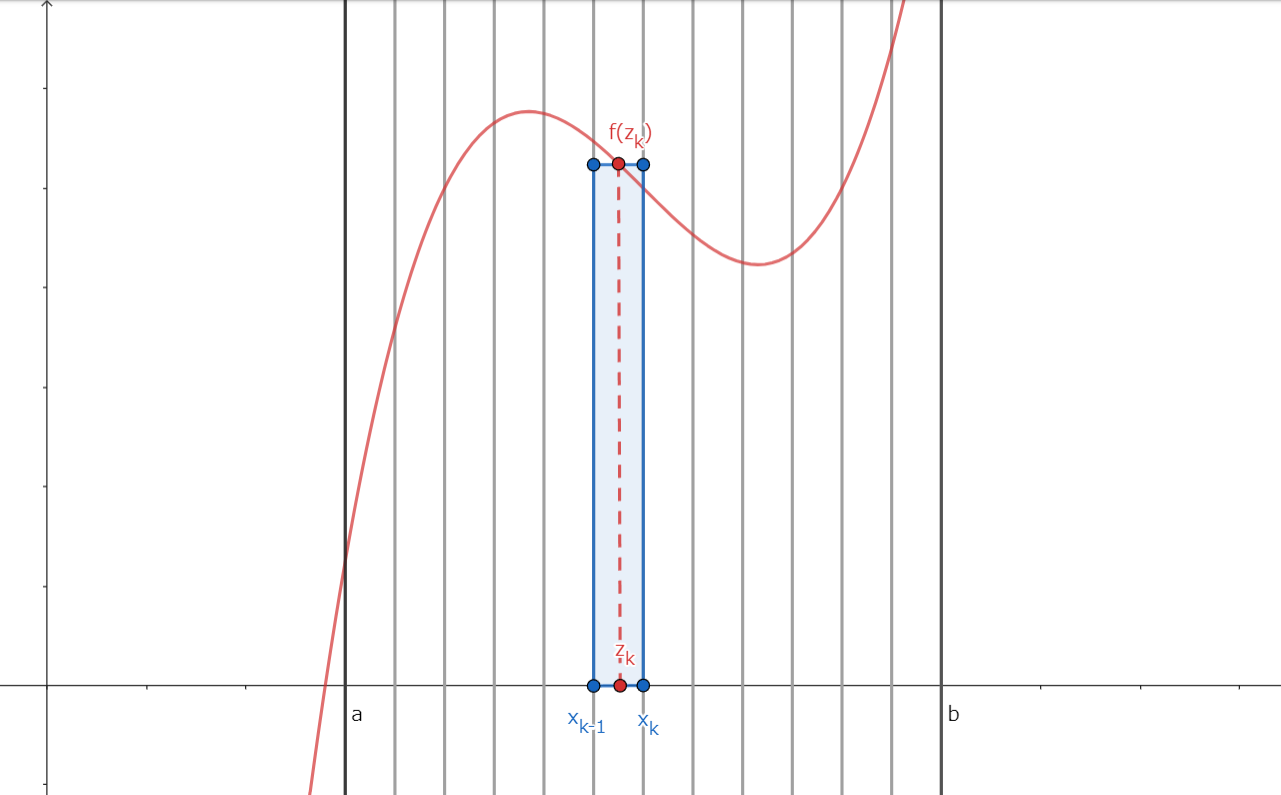
\includegraphics[scale=0.35]{img/QuuNote/integral_picture.png}
                    \caption{定積分の定義}\label{fig:定積分図}
                \end{figure}

                記号$\int_a^b f(x)dx$について、$a,b$をそれぞれ積分下限、積分上限という。また、変数$x$を\textbf{積分変数}という。
                定積分は数値であるので、積分変数によってその結果は変わらない。すなわち
                \begin{equation}
                    \int_a^b f(x)dx = \int_a^b f(t)dt
                \end{equation}
                のように、積分変数を$x$としても$t$としても同じである。式\eqref{eq:定積分の定義}について、右辺の極限が存在するとき、
                $f(x)$は\textbf{積分可能である}という。$f(x)$が連続関数ならば常に積分可能である。

                先ほどの過程では$f(x)\geq0$としてきたが、もちろん$f\leq0$の場合でも同様に定義される。積和の定義から、$f\leq0$であれば
                定積分は``負''の面積を与えることがわかる。
                \clearpage
                さて、試しに$f(x)=c(\text{定数})$の場合の定積分を求めてみよう。これは長方形の面積を求めることになるから当然答えは$c(b-a)$である。
                \begin{equation*}
                    \int_a^b cdx = \lim_{n\to 0}\sum_{k=1}^{n} c\Delta x_k = c\lim\sum (x_{k}-x_{k-1})
                \end{equation*}
                あとは$\Sigma$の定義から
                \begin{equation*}
                    c\lim\sum (x_k-x_{k-1})=c\lim\left\{(x_1-x_0)+(x_2-x_1)+\cdots+(x_{n-1}-x_{n-2})+(x_n-x_{n-1})\right\}=c\lim (x_{n}-x_0)
                \end{equation*}
                $x_n=b,x_0=a$であるから結局
                \begin{equation}
                    \int_a^b cdx = c(b-a) \label{eq:int_cdx}
                \end{equation}
                となる。なお、上記のように$\sum,\lim$の記号を一部省略して書くことはしばし用いられる。このノートでも以降頻繁に用いる。

                $f(x)=c$というもっとも単純な場合でさえこの計算量なのだから、$f$がもっと複雑になると計算量も途方のないものになる。しかし安心してほしい。
                数値計算等を除いて式\eqref{eq:定積分の定義}を用いて積分を計算することはほとんどない。実はもっと賢いやり方が存在するのである。
            \clearpage
            \subsection{定積分の性質}
                ここでは定積分の諸性質についてまとめる。仮定として$f,g$は区間$[a,b]$で連続であるとする。
                \begin{enumerate}\setcounter{enumi}{0}\renewcommand{\labelenumi}{(\arabic{enumi})}
                    \item $\displaystyle \int_a^b \left\{f(x)\pm g(x)\right\}dx=\int_a^b f(x)dx\pm\int_a^b g(x)dx\label{eq:定積分の加法性}$
                    \item $\displaystyle \int_a^b cf(x)dx=c\int_a^b f(x)dx \quad (c\text{は定数})$
                    \item $x\in [a,b]$で$f\geq 0$ならば$\displaystyle\int_a^b f(x)dx\geq 0 \label{eq:被積分関数が正なら面積も正}$
                    \item $x\in [a,b]$で$f\geq g$ならば$\displaystyle\int_a^b f(x)dx\geq \int_a^b g(x)dx\label{eq:関数と積分値の大小関係}$
                    \item $\displaystyle \int_a^b f(x)dx = f(c)(b-a)\quad (c\in (a,b))\label{eq:積分の平均値の定理}$
                    \item $\displaystyle \int_a^bf(x)dx=\int_a^c f(x)dx+\int_c^b f(x)dx \quad(c\in(a,b))\label{eq:定積分の区間についての加法性}$
                    \item $\displaystyle \int_a^b f(x)dx = -\int_b^a f(x)dx\label{eq:int[a,b]=-[b,a]}$
                    \item $\displaystyle \int_a^a f(x)dx=0\label{eq:int[a,a]=0}$
                    \item $\displaystyle \left|\int_{a}^{b}f(x)dx\right|\leq \int_{a}^{b}|f(x)|dx$\label{eq:積分の三角不等式}
                \end{enumerate}
                式\eqref{eq:積分の平均値の定理}は(積分の)\textbf{第一平均値定理}\footnote{平均値の第一定理とも。文脈によっては単に平均値の定理とも呼ぶこともある。}と呼ばれる。性質\eqref{eq:int[a,b]=-[b,a]}は性質というよりは
                このように定める(定義)として考えるとよい。\footnote{線積分を学ぶと、この定義が見通しよくなる。なぜなら左辺は$C:a\to b$の曲線に沿った積分$\int_C$であるためである。}数学書の中にはこれを証明させるものもあるが気にしなくてよい。性質\eqref{eq:定積分の区間についての加法性}も同様である。
                性質\eqref{eq:定積分の加法性},\eqref{eq:被積分関数が正なら面積も正}と\eqref{eq:int[a,b]=-[b,a]}から性質\eqref{eq:関数と積分値の大小関係}と性質\eqref{eq:int[a,a]=0}は容易に証明できるので演習問題とする。よって\eqref{eq:積分の平均値の定理}とを示す。\footnote{なお、性質\eqref{eq:積分の三角不等式}も簡単に示せる。時間がある人はやってみよう。}

                \paragraph{平均値の定理の証明}
                    $f(x)$が定数関数なら明らかに式\eqref{eq:積分の平均値の定理}が成り立つ。よって$f(x)$は区間$[a,b]$で最大値$M$と最小値$m$を取るとする。この時
                    \begin{equation*}
                        m\leq f(x) \leq M
                    \end{equation*}
                    である。性質\eqref{eq:関数と積分値の大小関係}より
                    \begin{equation*}
                        \int_a^b mdx \leq \int_a^b f(x)dx \leq \int_a^b Mdx
                    \end{equation*}
                    $m,M$は$x$によらない定数なので
                    \begin{equation*}
                        m(b-a) \leq \int f(x)dx \leq M(b-a)
                    \end{equation*}
                    各辺を$b-a$で割ると
                    \begin{equation*}
                        m \leq \frac{1}{(b-a)}\int_a^b f(x)dx \leq M
                    \end{equation*}
                    $f(x)$は$[a,b]$で連続関数だから、中間値の定理\eqref{eq:中間値の定理}より、
                    \begin{equation*}
                        \frac{1}{b-a}\int_a^b f(x)dx = f(c)
                    \end{equation*}
                    となるような点$c$が区間$(a,b)$内に存在する。よって、平均値の定理\eqref{eq:積分の平均値の定理}が証明された。$\square$
                平均値の定理はしばし次のように書くこともある。
                \begin{equation}
                    \int_{a}^{b}f(x)dx = (b-a)f(a+\theta(b-a))\quad (0<\theta < 1) \label{eq:積分の平均値の定理θ}
                \end{equation}
                これは$\theta$をラグランジュの平均値の定理\eqref{eq:平均値の定理1}と同じように使っている。

                性質\eqref{eq:定積分の区間についての加法性}では$a<c<b$としているが、性質\eqref{eq:int[a,b]=-[b,a]}を規約することで、この条件がなくても
                常に\eqref{eq:定積分の区間についての加法性}が成り立つ。

                \vspace{\stretch{1}}
                \hrulefill

                余談だが、
                \begin{equation*}
                    \int_I dx = \int_{a}^{b}dx = b-a
                \end{equation*}
                は$I=[a,b]$の長さを表す。同様にして二重積分についても
                \begin{equation*}
                    \iint _D dx dy = S(D)
                \end{equation*}
                は領域$D$の面積$S(D)$を表す。ここまでくればもちろん三重積分についても
                \begin{equation*}
                    \iiint _D dx dy dz = V(D)  
                \end{equation*}
                が領域$D$の体積$V(D)$だと予想がつく。(実際そうである。)このノートや高専2年生では多重積分のタの字も出てこないが、
                こういうちょっとした知識を学ぶだけでも楽しい。
            \clearpage
            \subsection{微積分学の基本定理}
                ここでは解析学上もっとも重要な定理(言いすぎ?)である微積分学の基本定理について述べる。最も重要なのでていねいに導出することにする。

                まず、関数$f(x)$について、$F(x)$を次のように定める。
                \begin{equation*}
                    F(x)=\int_a^x f(x)dx
                \end{equation*}
                このとき、$F(x+\Delta x)$は区間の加法性\eqref{eq:定積分の区間についての加法性}より
                \begin{equation*}
                    F(x+\Delta x)=\int_a^{x+\Delta x}=\int_a^x + \int_{x}^{x+\Delta x}=F(x)+\int_x^{x+\Delta x}f(x)dx
                \end{equation*}
                よって、移項して平均値の定理\eqref{eq:積分の平均値の定理θ}より
                \begin{equation*}
                    F(x+\Delta x)-F(x)=\Delta xf(x+\theta\Delta x)\quad (0<\theta<1)
                \end{equation*}
                式を整理すると
                \begin{equation*}
                    f(x+\theta \Delta x) = \frac{F(x+\Delta x)-F(x)}{\Delta x}
                \end{equation*}
                ここで、$\Delta x\to 0$の極限を取ると
                \begin{equation*}
                    f(x)=F'(x)
                \end{equation*}
                すなわち
                \begin{equation}
                    f(x)=\frac{d}{dx}\int_a^x f(x)dx\label{eq:微積分学の基本定理}
                \end{equation}
                これが\textbf{微積分学の基本定理}である。この定理は微分と積分が互いに逆の演算であることを示している。
                すなわち$F$は$f$の原始関数になる。$f$が\underline{連続であれば}それが可能なのである。

                $F$が$f$の原始関数であるということは$F+C$も$f$の原始関数である。
                \begin{equation*}
                    F(x)+C = \int_a^x f(x)dx
                \end{equation*}
                ここで$x=a$とすると性質\eqref{eq:int[a,a]=0}より
                \begin{equation*}
                    F(a)+C=0 \leftrightarrow C=-F(a)
                \end{equation*}
                よって、$x=b$とすれば
                \begin{equation}
                    \int_a^b f(x)dx = F(b)-F(a) \label{eq:微積分学の第二基本定理} 
                \end{equation}
                これを\textbf{微積分学の第二基本定理}という。この表現に倣って\eqref{eq:微積分学の基本定理}は微積分学の第一基本定理と呼ばれる。

                式\eqref{eq:微積分学の第二基本定理}の右辺は次の便利な表記法がある。
                \begin{equation*}
                    \left[F(x)\right]_a^b = F(x)\left|_a^b\right. = F(b)-F(a)
                \end{equation*}
                \clearpage
                不定積分については、以前すでに不完全であるが定義した。そこで、本当の不定積分の定義を述べようと思う。そもそも、不定積分は
                定数分の不定性はなく、ある点$a$で固定して定義される。\footnote{本によっては、$\int_a^x$と$\int_b^x$は定数分の差しかないので下限を省略して$\int $を不定積分と定義するものもある。}
                \begin{equation}
                    F(x)=\int_{a}^{x}f(x)dx
                \end{equation}
                これが点$a$における不定積分の定義である。ちなみにイギリスかどこかの数学書では不定積分を
                \begin{equation*}
                    \int^x f(x)dx
                \end{equation*}
                と表記するらしい。

                定積分の計算で公式\eqref{eq:微積分学の第二基本定理}を用いるときは、積分範囲に気を付けなければならない。例えば、
                \begin{equation*}
                    \int_{-1}^{1} \frac{dx}{x} = \left[\log|x|\right]_{-1}^1=\log|1|-\log|-1|=0
                \end{equation*}
                と行うのは不適である。被積分関数が$x=0$で不連続になってしまうからである。多価関数の場合は、関数が連続になるように
                分枝を取らなければならない。
            \clearpage
            \subsection{定積分の計算}
                ここでは定積分の計算について述べる。
                \paragraph{置換積分法}
                    関数$x=\phi(t)$について、$\phi(t)$と$\phi'(t)$が$[\alpha,\beta]$で連続であり$a=\phi(\alpha),b=\phi(\beta)$とする。このとき
                    \begin{equation}
                        \int_{a}^{b}f(x)dx = \int_{\alpha}^{\beta}f(\phi(t))\phi'(t)dt\label{eq:置換積分_定積分}
                    \end{equation}
                    が成りたつ。これを置換積分という。

                    公式\eqref{eq:置換積分_定積分}の証明を行おう。
                    \begin{equation*}
                        F(x)=\int_{a}^{x}f(x)dx
                    \end{equation*}
                    と置くと
                    \begin{equation*}
                        \frac{dF}{dt}=\frac{dF}{dx}\frac{dx}{dt}=f(x)\phi'(t)
                    \end{equation*}
                    であるため、両辺を$\int_{\alpha}^{\beta}$で積分すると
                    \begin{equation*}
                        F(\phi(\beta))-F(\phi(\alpha))=\int_{\alpha}^{\beta}f(\phi(t))\phi'(t)dt
                    \end{equation*}
                    左辺は$F(b)-F(a)=\int_a^b $であるため、公式\eqref{eq:置換積分_定積分}を得る。

                \paragraph{部分積分法}
                    関数$f,g$について、どちらの関数も$[a,b]$で微分可能であり、$f',g'$が連続であれば
                    \begin{equation}
                        \int_a^b f(x)g'(x)dx = \left[f(x)g(x)\right]_a^b - \int_a^b f'(x)g(x)dx \label{eq:部分積分_定積分}
                    \end{equation}
                    が成り立つ。これを部分積分という。

                    公式\eqref{eq:部分積分_定積分}の証明を行う。まず、明らかに次が成り立つ。
                    \begin{equation*}
                        (fg)' = fg' + f'g
                    \end{equation*}
                    よって、移項すれば
                    \begin{equation*}
                        fg' = (fg)' - f'g
                    \end{equation*}
                    ここで両辺を$\int_a^b$で積分すれば公式\eqref{eq:部分積分_定積分}を得る。\\

                    まとめると、置換積分も部分積分も、不定積分のときとやっていることは変わらない。積分区間等に気を付けさえいれば不定積分と同様に
                    計算してよいのである。これも基本定理のもたらした恩恵である。
            \clearpage
            \subsection{広義積分}
                ここでは定積分の定義を拡張した広義積分を扱う。具体的には次の二つの場合を扱う。
                \begin{enumerate}
                    \item 積分区間内で不連続な点が有限個存在する
                    \item 積分上限・下限の片方もしくは両方がが無限大である
                \end{enumerate}
                今までの仮定では被積分関数は区間内で連続であったが、この広義積分では不連続な点(有限個)や区間が無限大など
                広義の意味での定積分を考えるのである。そういう意味で広義積分というわけである。

                \paragraph{被積分関数が不連続}
                    $f(x)$が$[a,b)$で連続であるとする。この時、極限
                    \begin{equation*}
                        \lim_{\varepsilon \to +0}\int_{a}^{b-\varepsilon}f(x)dx
                    \end{equation*}
                    が存在すれば、その極限値を
                    \begin{equation*}
                        \int_{a}^{b}f(x)dx
                    \end{equation*}
                    と表す。同様に$(a,b]$で連続である場合も、極限
                    \begin{equation*}
                        \lim_{\varepsilon\to +0}\int_{a+\varepsilon}^{b}f(x)dx
                    \end{equation*}
                    が存在すれば、その極限値を
                    \begin{equation*}
                        \int_{a}^{b}f(x)dx
                    \end{equation*}
                    このようにすれば$a\leq c \leq b$であるような$x=c$において$f(x)$が不連続である場合は、下の右辺の極限が存在すると仮定すると
                    \begin{equation*}
                        \int_{a}^{b}f(x)dx = \lim_{\varepsilon_1\to +0}\int_{a}^{c-\varepsilon_1}f(x)dx+\lim_{\varepsilon_2\to +0}\int_{c+\varepsilon}^{b}f(x)dx
                    \end{equation*}       
                    と計算すればよいことがわかる。このとき$\varepsilon_1,\varepsilon_2$はそれぞれ独立に極限を取ることに注意。\footnote{一方で$\varepsilon_1=\varepsilon_2$として極限を取ることもある。これをコーシーの主値積分という。}\\
                    上記の極限が収束するとき、\textbf{広義積分は収束する}という。\footnote{実際に広義積分が収束するのを示すためには、よくコーシーの収束条件を使われる。}\\

                    例えば、$1/\sqrt{x}$は$x=0$で不連続であるが、
                    \begin{equation*}
                        \int_{0}^{1}\frac{dx}{\sqrt{x}}=\lim_{\varepsilon\to +0}\int_{\varepsilon}^{1}\frac{dx}{\sqrt{x}}=\lim_{\varepsilon\to+0}\left[2\sqrt{x}\right]_{\varepsilon}^1=\lim_{\varepsilon\to +0}2-2\sqrt{\varepsilon}=2
                    \end{equation*}
                    よって、広義積分は収束してその値は$2$である。一方で$1/x$について$[-1,1]$で積分すると$x=0$で不連続であることに注意すれば
                    \begin{equation*}
                        \int_{-1}^{1}\frac{dx}{x}=\lim_{\substack{\varepsilon_1\to +0\\\varepsilon_2\to +0}}\int_{-1}^{-\varepsilon_1}\frac{dx}{x}+\int_{\varepsilon_2}^{1}\frac{dx}{x}=\lim_{\substack{\varepsilon_1\to +0\\\varepsilon_2\to +0}}\left(\log\varepsilon_1-\log\varepsilon_2\right)
                    \end{equation*}
                    である。この極限は存在しない(発散する)ので、広義積分は収束しない。つまりは$\displaystyle \int_{-1}^{1}\frac{dx}{x}$は無意味。
                \clearpage
                \paragraph{積分区間が無限大}
                    関数$f(x)$が$x\geq a$で連続であるとする。このとき極限
                    \begin{equation*}
                        \lim_{b\to \infty}\int_{a}^{b}f(x)
                    \end{equation*}
                    が存在すれば、それを
                    \begin{equation*}
                        \int_{a}^{\infty}f(x)dx
                    \end{equation*}
                    と表す。同様にして
                    \begin{align*}
                        \int_{-\infty}^{b}f(x)dx=\lim_{a\to -\infty}\int_{a}^{b}f(x)dx\\
                        \int_{-\infty}^{\infty}f(x)dx=\lim_{\substack{a\to -\infty\\b\to\infty}}\int_{a}^{b}f(x)dx
                    \end{align*}
                    も定義される。\\
                    上式の極限が収束するとき、\textbf{広義積分は収束する}という。\\

                    これも例を挙げてみよう。例えば
                    \begin{equation*}
                        \int_{0}^{\infty}\frac{dx}{1+x^2}=\lim_{b\to\infty}\int_{0}^{b}\frac{dx}{1+x^2}=\lim_{b\to\infty}\left[\arctan(x)\right]_0^b=\lim_{b\to\infty}\arctan b=\frac{\pi}{2}
                    \end{equation*}
                    と計算できる。ちなみにこの結果、すなわち$1/(1+x^2)$の$[0,\infty)$の広義積分が$\pi/2$になるという事実は覚えておくとよい。
                    一方で、
                    \begin{equation*}
                        \int_{1}^{\infty}\frac{dx}{\sqrt{x}}=\lim_{b\to\infty}\int_{1}^{b}\frac{dx}{\sqrt{x}}=\lim_{b\to \infty}\left[2\sqrt{x}\right]_1^b=\lim_{b\to \infty}2(\sqrt{b}-1)
                    \end{equation*}
                    は右辺の極限が発散するので、広義積分$\displaystyle\int_{1}^{\infty}\frac{dx}{\sqrt{x}}$は意味を持たないことがわかる。\\

                    今あげた計算を見れば、広義積分について大まかに理解できると思う。本来連続な区間でしか定義していない定積分を不連続点を含む区間や、無限区間で
                    定義することがわかればよい。どちらの場合にせよ、連続な区間に分けて最後に極限を取るのである。このことを\underline{十分理解できている}なら、実際の計算では
                    \begin{equation*}
                        \int_{0}^{\infty}\frac{dx}{1+x^2}=\left[\arctan x\right]_0^\infty = \frac{\pi}{2}
                    \end{equation*}
                    と略記してもよい。無限区間の積分は、この微分積分以外にも当たり前のように顔を出す。ぜひともこの機会に慣れておきたいものである。
            \clearpage
            \basicquestion 以下の問いに答えよ。
                \paragraph{問1}定積分の性質\eqref{eq:定積分の加法性},\eqref{eq:被積分関数が正なら面積も正}を用いて性質\eqref{eq:関数と積分値の大小関係}を、性質\eqref{eq:int[a,b]=-[b,a]}を用いて性質\eqref{eq:int[a,a]=0}を示せ。

                \paragraph{問2}定積分の定義より$\int_{0}^{1}xdx$を計算せよ。ただし$z_k=x_k$とし、$[0,1]$は丁度$n$等分するものとする。

                \paragraph{問3}以下の定積分の値を求めよ。ただし$0\leq \epsilon < 1$である。\\
                $(1)\displaystyle \int_{0}^{\pi}\sin x dx$\hspace{3mm}%それにしてもあのsinの曲線下の面積がこんなに簡単に求まるなんて、ただただ驚くばかりである。
                $(2)\displaystyle \int_{0}^{\frac{1}{2}}\frac{dx}{\sqrt{1-x^2}}$\hspace{3mm}
                $(3)\displaystyle \int_0^2 x^2e^{x}dx$\hspace{3mm}
                $(4)\displaystyle \int_{-3}^3\left(x^5+x^4+x^3+x^2+5\right)dx$\hspace{3mm}
                $(5)\displaystyle \int_0^\pi \frac{dx}{1+\epsilon\cos x}$

                \paragraph{問4}次の広義積分を求めよ。\\
                $(1)\displaystyle \int_{-1}^{-\infty}\frac{dx}{x^4}$\hspace{3mm}
                $(2)\displaystyle \int_0^1 \log xdx$\hspace{3mm}
                $(3)\displaystyle \int_0^1 \frac{dx}{x\log x}$\hspace{3mm}
                $(4)\displaystyle \int_0^a \frac{dx}{\sqrt{ax-x^2}}\quad(a>0)$\hspace{3mm}
                $(5)\displaystyle \int_0^\infty \frac{dx}{x^3+1}$

                \paragraph{問5}以下の式を示せ。ただし$m,n$は正整数とする。
                \begin{equation*}
                    \int_{0}^{2\pi}\cos mx\cos nx dx = \begin{cases}
                        0 & (m\neq n)\\ \pi & (m=n)
                    \end{cases}
                \end{equation*}

                \paragraph{問6}次の積分(広義積分)が収束するための$k$の範囲を求めよ。
                \begin{equation*}
                    \int_1^\infty \frac{dx}{x^{k}}
                \end{equation*}

                \paragraph{問7}関数$f(x)$が偶関数であることを$f=f_e$、奇関数であることを$f=f_o$と表記することにする。この時以下を示せ。
                \begin{equation}
                    \int_{-a}^a f(x)dx = \begin{cases}
                        \displaystyle 2\int_{0}^{a}f(x)dx & (f=f_e) \\ 0 & (f=f_o)
                    \end{cases}\label{eq:定積分と偶関数・奇関数}
                \end{equation}

                \paragraph{問8}次の問いに答えよ。
                \begin{enumerate}\setcounter{enumi}{0}\renewcommand{\labelenumi}{(\arabic{enumi})}
                    \item $\displaystyle \int_0^\pi \frac{\sin x}{1+\cos^2 x}dx$を求めよ。
                    \item $x\to\pi -x$の置換により$\displaystyle \int_{0}^{\pi}xf(\sin x)dx=\frac{\pi}{2}\int_{0}^{\pi}f(\sin x)dx$を示せ。\\ただし、$f(\sin x)$は$\sin x$の有理関数である。
                    \item $\displaystyle \int_{0}^{\pi} \frac{x\sin x}{1+\cos^2 x}dx$を求めよ。
                \end{enumerate}
            \clearpage
        \section{積分法の応用}
            \subsection{面積・体積} 
                ここからは定積分の応用を述べる。まずは定積分を用いて面積・体積を求める。面積については、定積分の定義を述べる際に
                触れたが、実は体積も求められる。

                関数$f(x)$と$g(x)$について、区間$[a,b]$で$f(x)\geq g(x)$となるとき、曲線$y=f,y=g$と直線$x=a,x=b$で囲まれた図形の面積は
                \begin{equation}
                    \int_{a}^{b} \left\{f(x)-g(x)\right\}dx \label{eq:曲線で囲まれた面積}
                \end{equation}
                特に、$f\leq 0$であれば
                \begin{equation}
                    -\int_a^b f(x)dx \label{eq:-負の面積}
                \end{equation}
                例として、円の面積を求めてみよう。半径$r$の半円の上部$y\geq 0$の面積は
                \begin{equation*}
                    S=\int_{-r}^{r}\sqrt{r^2-x^2}dx
                \end{equation*}
                で与えられる。$x=r\sin\theta$の置換を行うと、$dx=r\cos\theta d\theta$であるため
                \begin{equation*}
                    S=\int_{-\frac{\pi}{2}}^{\frac{\pi}{2}}\sqrt{r^2-r^2\sin^2\theta}\cdot r\cos\theta d\theta=r^2\int_{-\frac{\pi}{2}}^{\frac{\pi}{2}}\cos^2\theta d\theta=2r^2\int_{0}^{\frac{\pi}{2}}\cos^2\theta d\theta
                \end{equation*}
                半角の公式$\displaystyle \cos^2\theta = \frac{1+\cos2\theta}{2}$であるため、
                \begin{equation*}
                    S=2r^2\int_{0}^{\frac{\pi}{2}}\frac{1+\cos 2\theta}{2}d\theta=2r^2\left[\frac{\theta+\frac{1}{2}\sin 2\theta}{2}\right]_0^{\frac{\pi}{2}}=\frac{\pi}{2}r^2
                \end{equation*}
                よって、円の面積の公式$\pi r^2$が導けた。

                次に体積を求めてみよう。x軸上のある点$x$において断面積$S(x)$であるとき、区間$[a,b]$での体積$V$は
                \begin{equation}
                    V=\int_a^b S(x)dx \label{eq:体積の公式}
                \end{equation}
                で求まる。もちろんこれだけではよくわからないだろうから、図を見て理解しよう。
                \begin{figure}[h]
                    \centering
                    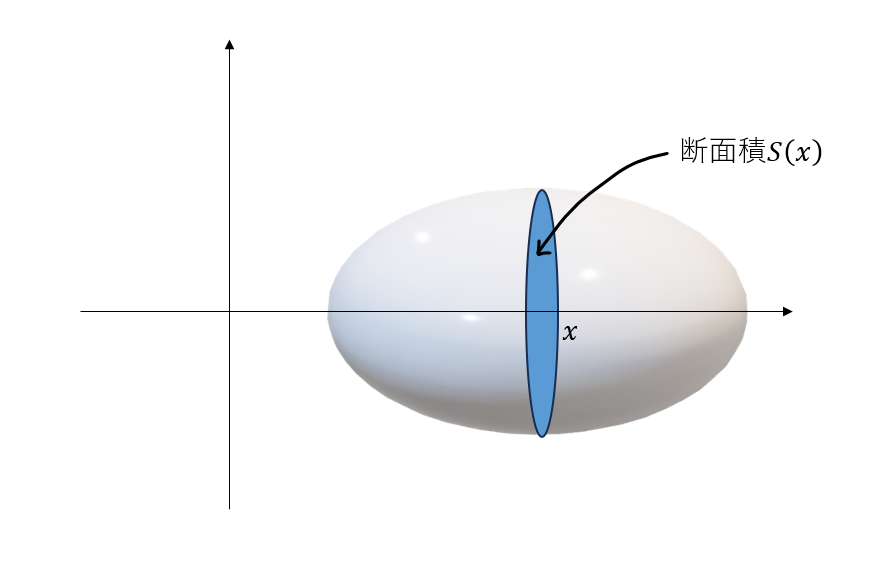
\includegraphics[scale=0.3]{img/QuuNote/Sx_V.png}
                    \caption{立体の体積と断面積}
                \end{figure}

                まず、公式中の断面積というのはx軸に垂直な平面で切った時の面積となる。これに$dx$を掛けた量$S(x)dx$は
                微小体積$dV$を表すことは容易に想像できる。その微小体積を$[a,b]$まで集めた($\int$した)ものが$V$となる。少し直感的な説明\footnote{安易に$dx$や$dV$といった量を出したが、これらはあいまいに使っていると感じると思う。ただ、$d$が「微小の」というニュアンスを持っていることはこれまでの話でなんとなく理解できるだろう。}になってしまったが、
                ここはイメージさえできればよい。

                公式\eqref{eq:体積の公式}を用いれば、$y=f(x)$をx軸で回転したときの回転体の公式も導出できる。これも図を見て考えればわかる。

                \begin{figure}[h]
                    \centering
                    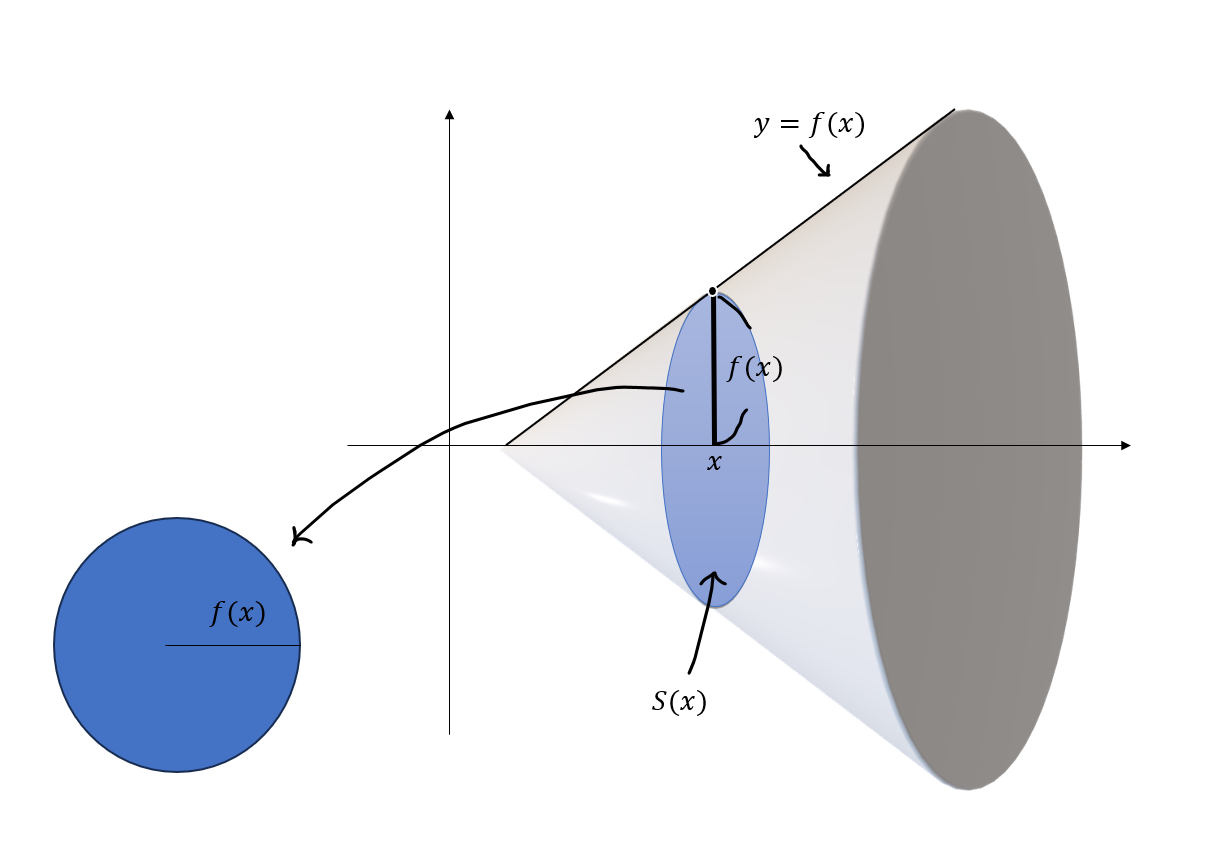
\includegraphics[scale=0.5]{img/QuuNote/rolling_Sx.png}
                    \caption{回転体の体積}
                \end{figure}

                図からわかるように、$y=f(x)$を回転させた回転体の断面積$S(x)$は円の面積の公式$\pi r^2$より$S(x)=\pi\left[f(x)\right]^2$となる。
                したがって、回転体の体積$V$は
                \begin{equation}
                    V=\pi\int_{a}^{b}\left[f(x)\right]^2 dx \label{eq:回転体の体積}
                \end{equation}
                で求まる。
            \clearpage
            \subsection{曲線の長さ}
                次に曲線$y=f(x)$の``長さ''を求めるとする。こちらは直感的な説明ではなく、より厳密に述べることにする。
                
                まず、区間$[a,b]$に分点$x_0=a,x_1,x_2,\dots,x_{n-1},x_n=b$を定め、$\Delta x_k=x_k - x_{k-1},\Delta y_k = f(x_k)-f(y_{k-1})$とする。
                この時、区間$[x_k,x_{k-1}]$の曲線の長さは($\Delta x_k$が十分小さいとすれば)$\displaystyle \Delta l_k = \sqrt{\Delta x_k^2+\Delta y_k^2}=\sqrt{1+\left(\frac{\Delta y_k}{\Delta x_k}\right)^2}\Delta x_k$と近似できる。
                ここで平均値の定理\eqref{eq:平均値の定理}より、
                \begin{equation*}
                    \Delta l_k=\sqrt{1+\left(\frac{\Delta y_k}{\Delta x_k}\right)}\Delta x_k = \sqrt{1+\left(\frac{dy}{dx}(z_k)\right)}\Delta x_k
                \end{equation*}
                となるような$x_{k-1}<z_k<x_k$が存在する。$y=f(x)$の区間$[a,b]$での曲線の長さは、分割の数$n$を限りなく大きくしたときの$\sum \Delta l_k$に等しいから
                \begin{equation}
                    \int_{a}^{b} \sqrt{1+\left(\frac{dy}{dx}\right)^2}dx \label{eq:曲線の長さ}
                \end{equation}
                となる。

                \begin{figure}[h]
                    \centering
                    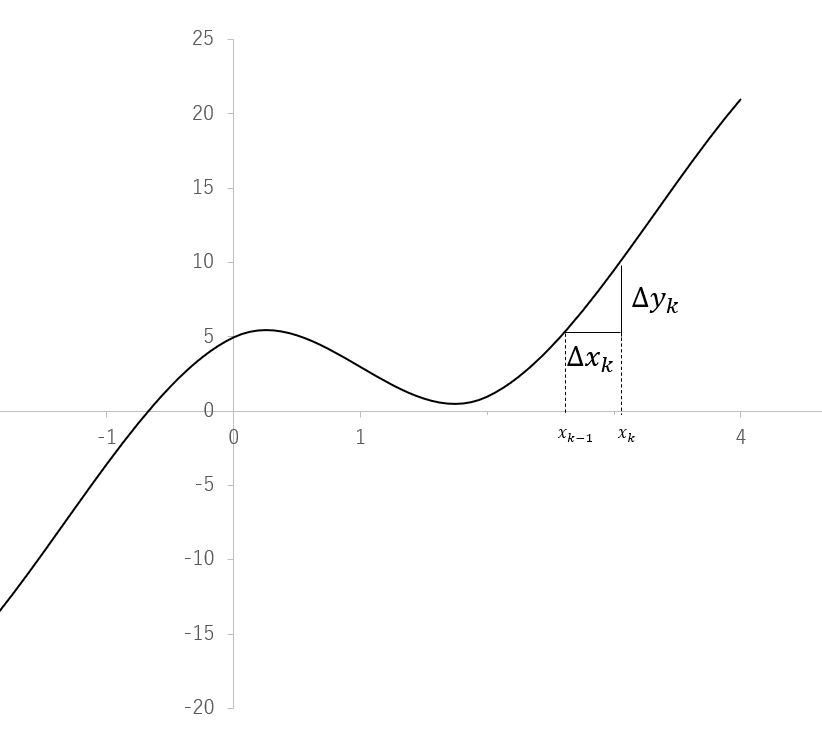
\includegraphics[scale=0.35]{img/QuuNote/curve_length.png}
                    \caption{曲線の長さ}
                \end{figure}

                これを使って、半径$r$の円周の長さを求めてみる。円の方程式$x^2+y^2=r^2$より、$\displaystyle \left(\frac{dy}{dx}\right)^2=\frac{x^2}{r^2-x^2}$だから
                \begin{equation*}
                    2\int_{-r}^{r}\sqrt{1+\frac{x^2}{r^2-x^2}}dx=4\int_{0}^{r}\frac{r}{\sqrt{r^2-x^2}}dx=4r\sin^{-1}\frac{r}{r}=2\pi r
                \end{equation*}
                最初の$\times 2$は、元の積分が半円の演習を求めていることによる。よって、円周の公式$2\pi r$が導けた。
            \clearpage
            \subsection{数値積分法}
                最後に数値積分法について簡単であるが述べる。これまでの計算では原始関数が簡単に求まるものばかりであったが、実際は原始関数を求めるのが難しいものもある。むしろそのほうが多いといってもいい。
                しかし、原始関数が求められなくても定積分なら(近似して)求められることもある(定義\eqref{eq:定積分の定義}参照)。
                ここでは近似計算の公式を紹介し、実際に面積を近似してみよう。なお、以降の計算では計算量の関係から関数電卓を用いることを
                強くすすめる。

                \paragraph{矩形法}まずはもっとも単純な矩形法から述べる。これは積分区間をある一定の幅(\textbf{刻み幅})で区切り、
                被積分関数を、その毎区間の左端での関数値で一定と近似して定積分を求める方法である。刻み幅を$h$と表すことにすれば、この表式は次のようになる。
                \begin{equation}
                    \int_{a}^{b}f(x)dx \approx \sum_{k=1}^{(b-a)/h}f(a+(k-1)h)\cdot h \label{eq:矩形法}
                \end{equation}
                こういうのは数式や説明を見るより、実際の計算を見たほうが理解しやすいだろう。$f(x)=x^2$の$[0,2]$の定積分を
                矩形法で計算してみる。刻み幅は$h=0.5$とする。
                \begin{equation*}
                    \int_{0}^{2}x^2 dx \approx f(0)\cdot h + f(0.5)\cdot h+f(1.0)\cdot h + f(1.5)\cdot h = 0+0.125+0.5+1.125=1.75
                \end{equation*}
                よって近似値は$1.75$である。実際の値は$\frac{8}{3}\approx 2.67$なので、精度はあまりよくない。刻み幅が大きすぎるのも原因であるが、矩形法自体近似計算としてよい計算方法ではないのもある。

                \paragraph{台形公式}次に、面積を台形の形で近似する方法を述べる。矩形法では長方形で近似するので、区間の右端の値と$f(a+(k-1)h)$との差が大きいと誤差が大きくなるのは容易に想像できるだろう。
                しかし、台形で近似すれば、その誤差は三角形$(a+(k-1)h,f(a+(k-1)h)),(a+kh,f(a+(k-1)h)),(a+kh,f(a+kh))$の分だけ小さくなるのである。
                
                \begin{figure}[h]
                    \centering
                    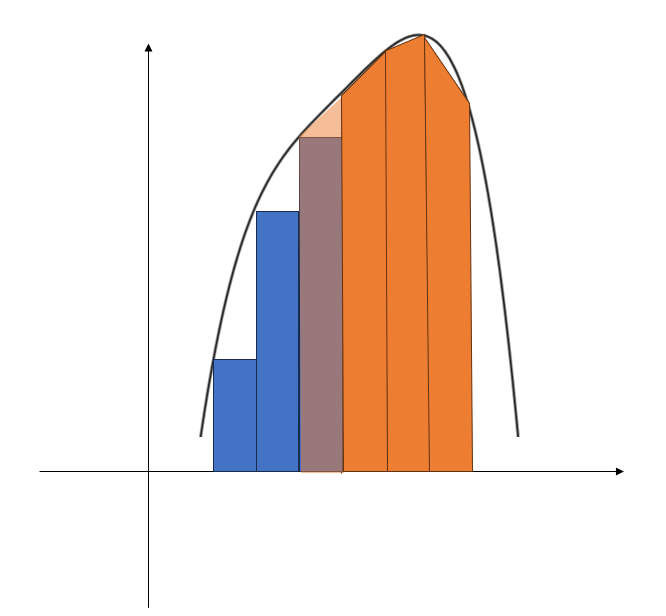
\includegraphics[scale=0.5]{img/QuuNote/trapezoidalRule.png}
                    \caption{矩形法(青)と台形近似(橙)の比較}\label{fig:矩形法と台形公式}
                \end{figure}

                分割の数を$n$とし、刻み幅を$h=\frac{b-a}{n}$とすると、図\ref{fig:矩形法と台形公式}からもわかるように各台形の面積は
                \begin{equation*}
                    \frac{1}{2}h(f(a+(k-1)h)+f(a+kh))
                \end{equation*}
                で表せられるのだから、この$n$個の台形面積の和を取れば
                \begin{equation*}
                    \frac{1}{2}h(f(a)+f(a+h))+\frac{1}{2}h(f(a+h)+f(a+2h))+\cdots+\frac{1}{2}h(f(a+(n-1)h)+f(b))
                \end{equation*}
                したがって、以下の\textbf{台形公式}が得られる。
                \begin{equation}
                    \int_{a}^{b}f(x)dx \approx \frac{h}{2}\left\{f(a)+2f(a+h+2f(a+2h)+\cdots+2f(a+(n-1)h)+f(b))\right\}\label{eq:台形公式}
                \end{equation}

                \paragraph{シンプソンの公式}最後にシンプソンの公式について述べる。こんどは面積を$n=2m$個の帯に分割する。もちろん刻み幅$h=(b-a)/n=(b-a)/2m$である。
                この帯を2つで一つのセットと考えれば、合計$m$個のセットができる。それぞれのセットについて、各点$P_{2k-2},P_{2k-1},P_{2k}$を通る放物線で近似することを考えると、
                面積は以下の式で与えられる。
                \begin{equation}
                    \frac{h}{3}\left\{f(a+(2k-2)h)+4f(a+(2k-1)h)+f(a+2kh)\right\} \label{eq:シンプソン各面積}
                \end{equation}
                
                \begin{figure}[h]
                    \centering
                    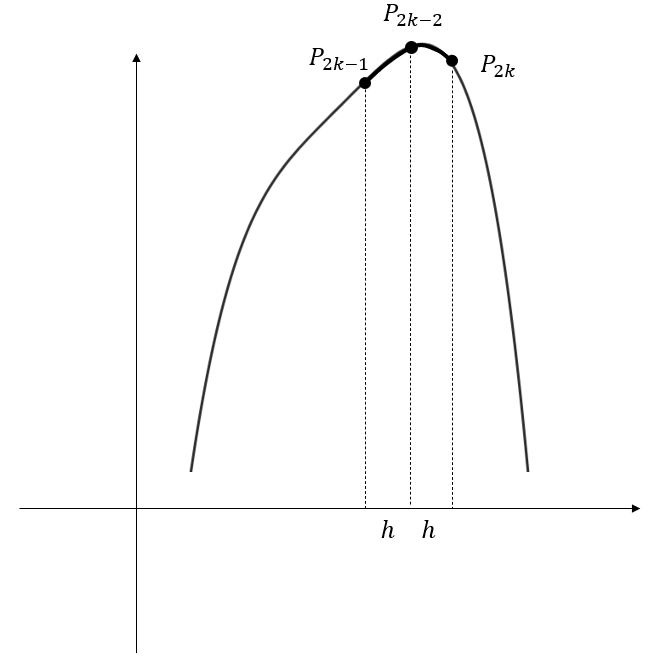
\includegraphics[scale=0.5]{img/QuuNote/simpsonLow.png}
                    \caption{シンプソンの公式}
                \end{figure}

                なぜなら、三点$\displaystyle Q_0(\alpha,y_0),Q_1\left(\frac{\alpha+\beta}{2},y_1\right),Q_2(\beta,y_2)$を通る放物線$y=Ax^2+Bx+C$の面積は
                \begin{equation*}
                    \int_{\alpha}^{\beta}ydx = \int_{\alpha}^{\beta} \left\{Ax^2+Bx+C\right\}dx = \frac{(\beta-\alpha)}{3}\left\{A(\alpha^2+\alpha\beta+\beta^2)+\frac{3}{2}+B(\beta+\alpha)+3C\right\}
                \end{equation*}
                となり、放物線は$Q_0,Q_1,Q_2$を通るから
                \begin{align*}
                    y_0 &= A\alpha^2+B\alpha+C \\
                    y_1 &= A\left(\frac{\alpha+\beta}{2}\right)^2+B\left(\frac{\alpha+\beta}{2}\right)+C\\
                    y_2 &= A\beta^2+B\beta+C 
                \end{align*}
                よって、
                \begin{equation*}
                    y_0+4y_1+y_2=2\left\{A(\alpha^2+\alpha \beta+\beta^2)+\frac{3}{2}B(\alpha+\beta)+3C\right\}
                \end{equation*}
                したがって、
                \begin{equation*}
                    \int_{\alpha}^{\beta}ydx=\frac{\beta-\alpha}{3}\left(y_0+4y_1+y_2\right)
                \end{equation*}
                が得られる。だから$Q_0=P_{2k-2},Q_1=P_{2k-1},Q_2=P_{2k}$と考えれば、各面積は式\eqref{eq:シンプソン各面積}で与えられるのである。

                長々と書いてしまったが、$m$個の面積を上記のように近似すれば、\textbf{シンプソンの公式}が得られる。
                \begin{equation}
                    \begin{split}
                        \int_{b}^{a}f(x)dx \approx &\frac{h}{3}\{f(a)+4f(a+h)+2f(a+2h)+4f(a+3h)+2f(a+4h)\\ &+\cdots+2f(a+(2m-2)h)+4f(a+(2m-1)h)+f(b)\}
                    \end{split}\label{eq:シンプソンの公式}
                \end{equation}\\

                今回は、数値積分法として三つの方法\footnote{なお、高専の情報基礎では矩形法のみ扱う。先生はシンプソンの公式などを紹介したそうであったが。}を紹介したが、式の複雑さからもわかるように最も誤差が小さく計算できるのはシンプソンの公式である。
                プログラミングの知識がある人はそれぞれの方法で計算して誤差を比較してみると楽しい。もちろん上記以外の数値積分の方法も存在する。気になったら調べてみるとよい。
            \clearpage
            \basicquestion 以下の問いに答えよ。

                \paragraph{問1}楕円$\displaystyle\frac{x^2}{a^2}+\frac{y^2}{b^2}=1\quad (a,b>0)$の面積を求めよ。

                \paragraph{問2}$y^2=4px$と$x^2=4py\quad (p>0)$で囲まれた図形の面積を求めよ。

                \paragraph{問3}半径$r$の球の体積の公式を導け。

                \paragraph{問4}カテナリー$y=\cosh x$の$-1\leq x\leq 1$での長さを求めよ。

                \paragraph{問5}底面の半径$r$、高さ$h$の円錐の体積の公式を導け。

                \paragraph{問6}$\displaystyle \int _0^1 \frac{4}{1+x^2}dx$を台形公式とシンプソンの公式を用いて求めよ。ただし、どちらも$n=4$とする。
            \clearpage
            \section{第III部演習問題}
            \paragraph{問1}以下の不定積分を求めよ。\\
                $\displaystyle [1]\int (x^2+1)^3dx$\hspace{3mm}
                $\displaystyle [2]\int x^2\cos xdx$\hspace{3mm}
                $\displaystyle [3]\int \frac{dx}{\sin x}$\hspace{3mm}
                $\displaystyle [4]\int \tan xdx$\hspace{3mm}
                $\displaystyle [5]\int \sin^5 xdx$
                $\displaystyle [6]\int \frac{dx}{\sqrt{(x-\alpha)(x-\beta)}}$\hspace{3mm}
                $\displaystyle [7]\int \frac{x^2}{(x+1)^2(x-2)}dx$\hspace{3mm}
                $\displaystyle [8]\int\frac{dx}{a^2\cos^2 x+b^2\sin^2 x}\quad(ab\neq 0)$ \hspace{5mm}
                $\displaystyle [9]\int \sqrt{1+\cos x}dx$
            
            \paragraph{問2}以下の定積分(広義積分も含む)を求めよ。\\
                $\displaystyle [1]\int_1^2\frac{5x^2-3x+4}{\sqrt{x}}dx$\hspace{3mm}
                $\displaystyle [2]\int_{-\infty}^{\infty}\frac{dx}{\cosh x}$\hspace{3mm}
                $\displaystyle [3]\int_1^e \frac{\sin(\pi\log x)}{x}dx$\hspace{3mm}
                $\displaystyle [4]\int_1^2 \frac{x-1}{x^2}e^xdx$\hspace{3mm}
                $\displaystyle [5]\int_0^1 \frac{dx}{(x^2+1)^{\frac{5}{2}}}$\hspace{3mm}
                $\displaystyle [6]\int_0^{\frac{\pi}{2}}|\sin x-2\cos x|dx$\hspace{3mm}
                $\displaystyle [7]\int_0^{\frac{\pi}{2}}\log\sin xdx$\hspace{3mm}
                $\displaystyle [8]\int_0^3\frac{dx}{(3-x)^{\frac{3}{2}}}$\hspace{3mm}
                $\displaystyle [9]\int_0^\infty e^{-wx}dx $\hspace{3mm}
                $\displaystyle [10]\int_0^1\frac{dx}{\left[ax+b(1-x)\right]^2}$
            
            \paragraph{問3}以下の図形の面積・体積を求めよ。
                \begin{enumerate}\setcounter{enumi}{0}\renewcommand{\labelenumi}{(\arabic{enumi})}
                    \item $y=\sin x,y=\cos x$と直線$x=0,\pi$に囲まれた図形の面積
                    \item $x^2+(y-a)^2 = r^2$をx軸周りに回転してできる立体(トーラス)の体積
                \end{enumerate}
            
            \paragraph{問4}$s>0$で定義される(実は複素数まで定義できる!)関数$\Gamma(s)$の定義は
                \begin{equation}
                    \Gamma(s) = \int_{0}^{\infty}x^{s-1}e^{-x}dx \label{eq:ガンマ関数}
                \end{equation}
                である。この$\Gamma(s)$を\textbf{ガンマ関数}という。この時以下を示せ。
                \begin{enumerate}\setcounter{enumi}{0}\renewcommand{\labelenumi}{(\arabic{enumi})}
                    \item $\Gamma(s+1)=s\Gamma(s)$
                    \item $\Gamma(n+1)=n!\quad (n\in \mathbb{N})$
                \end{enumerate}

            \paragraph{問5}$m,n$を負でない整数とするとき、次の積分を求めよ。
                \begin{equation*}
                    \int_0^1 x^m(1-x)^ndx
                \end{equation*}

            \paragraph{問6}$n=0,1,2,\dots$とするとき、次の定積分を求めよ。
                \begin{equation*}
                    G_{n}=\int_{-\infty}^{\infty}x^{n}e^{-x^2}dx
                \end{equation*}
                ただし、$\displaystyle \int_{-\infty}^{\infty}e^{-x^2}dx=\sqrt{\pi}$(\textbf{ガウス積分})は用いてよい。

            \paragraph{問7}$x$と$\sqrt{ax^2+bx+c}\quad(a>0)$の有理関数$f(x,\sqrt{ax^2+bx+c})$について、$t=\sqrt{ax^2+bx+c}+\sqrt{a}x$と置換することにより
                \begin{equation*}
                    \int f(x,\sqrt{ax^2+bx+c})dx
                \end{equation*}
                は必ず積分できることを示せ。
            \clearpage
            \paragraph{問8}以下の問いに答えよ。
            \begin{enumerate}\setcounter{enumi}{0}\renewcommand{\labelenumi}{(\arabic{enumi})}
                \item $n=0,1,2,\dots$とするとき
                    \begin{equation*}
                        I_n=\int_{n\pi}^{(n+1)\pi}dxe^{-x}\sin x
                    \end{equation*}を求めよ。
                \item 以下の積分を求めよ。
                    \begin{equation*}
                        I=\int_{0}^{\infty}dx e^{-x}|\sin x|
                        \end{equation*}
            \end{enumerate}

            \paragraph{問9}以下の$g(x)$について、$g'(x)$を求めよ。
                \begin{equation*}
                    g(x)=\int_{0}^{x}f(t)\cos(x+t)dt
                \end{equation*}
                
            \paragraph{問10}%mynote 59参照
                半径$r$の直円柱について、底面の直径$AB$を通り、平面と$\frac{\pi}{4}$の角をなす平面で切るとき、
                底面と平面の間の部分の体積$V$を以下の指示に従って求めよ。
                \begin{enumerate}
                    \item 底面の円周上の点$P$と円の中心$O$とがなす角を$\theta$とする(下図参照)。このとき、直径$AB$に対して垂直な平面で図形を切った時の断面積を$\theta$を用いて表せ。
                    \item $\theta$を十分小さな$\Delta \theta$だけ動かした点の位置を$P'$とするとき、この体積の微小変化分$\Delta V$を求めよ。
                    \item 立体の体積$V$を求めよ。
                \end{enumerate}
                \begin{figure}[h]
                    \centering
                    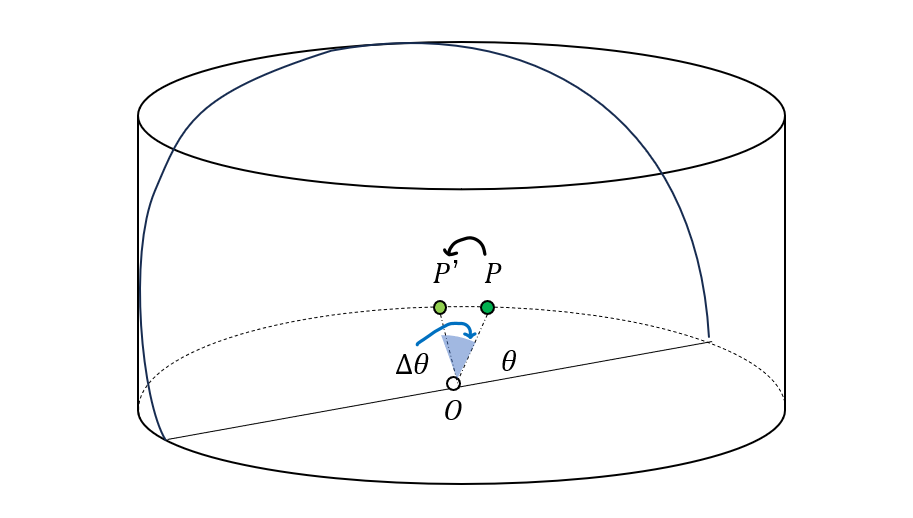
\includegraphics[keepaspectratio,scale=0.5]{img/QuuNote/questionForIntegral.png}
                    \caption{直円柱を平面で切る}
                \end{figure}
            \linktoMOKUZI
    \clearpage

    \part{無限級数$\sum$}
    \vspace{\stretch{1}}
    \begin{screen}
        いよいよ最後の部である無限級数に入る。ここでは主に無限級数が収束するかどうかの判定がメインになる。収束の判定には様々な方法があるが、まずは自分が気に入ったもの一つを会得するのがよいだろう。
        また、ここではべき級数についても扱う。べき級数には収束する範囲内において``一様収束''するという性質がある。この一様収束という概念がとっつきにくいが、
        これを満たす関数級数は微分積分の観点において非常によい性質を持っているのである。無限級数の話はこれから先の数学等でもひんぱんに用いられる非常に重要なものの基礎である。
        これを土台にして複素関数論・フーリエ級数・微分方程式も発展している。
    \end{screen}
    \clearpage
        \section{無限級数とは}
            \subsection{無限級数の定義}
                まずは、無限級数の定義について述べよう。まず無限数列を$\left\{a_n\right\}=a_1,a_2,a_3,\dots$とする。このとき、これらの和を取り
                \begin{equation}
                    a_1+a_2+a_3+\dots \label{eq:無限級数の直感的な定義}
                \end{equation}
                を考え、これを
                \begin{equation}
                    \sum_{n=1}^{\infty}a_n,\quad \sum_{n} a_n,\quad \sum a_n \label{eq:無限級数の書き方}
                \end{equation}
                とかく。これを\textbf{無限級数}または単に級数と呼ぶ。無限級数の書き方は上記の三つが主であるが、もちろん最初の書き方が一番丁寧である。

                加法は通常有限の項に対して定義されるので、上記の定義は形式なものになる。そこで、$\left\{a_n\right\}$の第$n$部分和$\left\{S_n\right\}$を
                \begin{equation*}
                    S_n = a_1+a_2+a_3+\cdots+a_n
                \end{equation*}
                と考えれば、式\eqref{eq:無限級数の直感的な定義}は、$S_n$の$n\to \infty$の極限を取ることと同じになる。よって、
                \begin{equation}
                    S=\lim_{n\to \infty}S_n
                \end{equation}
                の極限値$S$が存在すれば、$S=\sum a_n$と書き、無限級数は\textbf{収束する}という。また、この$S$を無限級数の和という。逆に、極限値が有限確定ではない場合、この級数は\textbf{発散する}という。\\

                以下に無限級数の性質を述べる。
                \begin{enumerate}
                    \item 無限級数の各項に0じゃない定数を書けても、その級数の収束or発散は変わらない。\\特に、$S=\sum a_n\leftrightarrow kS=\sum k a_n$
                    \item 級数に有限個の項を足し引きしても、その級数の収束or発散は変わらない。
                    \item $\sum a_n$が収束するならば$\lim a_n=0$
                \end{enumerate}
                特に性質3が重要で、これを言い換えると「$\lim a_n \neq 0 \rightarrow \sum a_n$は発散」となる。これを用いれば、級数が発散するかどうか調べることができる。注意しなければいけないのは、
                これの逆について、すなわち$\lim a_n=0$のときについては何も言及していないことである。すなわち、たとえ$a_n$が0に収束しようとも、その近づき方があまりにもゆっくりだった場合は級数が発散してしまうのである。

                例えば、$a_n=\sqrt{n+1}-\sqrt{n}$は、$\lim a_n = 0$であるが、
                \begin{equation*}
                    S_n = a_1+a_2+\cdots+a_n = (\sqrt{2}-\sqrt{1})+(\sqrt{3}-\sqrt{2})+\cdots+(\sqrt{n+1}-\sqrt{n})=\sqrt{n+1}-1
                \end{equation*}
                であるため、$S_n=\sum a_n$は発散してしまう。
            \clearpage
            \subsection{単調で有界な数列}
                次節以降で無限級数の収束を判定する方法等について述べるために、ここでは数列の補足を行う。\\

                まずは、有界について説明しよう。すべての$n$について、$a_n\leq M$となる定数$M$が存在するとき、
                数列$\{a_n\}$は\textbf{上に有界}であるという。この時の$M$を\textbf{上界}という。一方、すべての$n$
                について、$m\leq a_n$となる定数$m$が存在するとき、$\{a_n\}$は\textbf{下に有界}であるという。この時の
                $m$を\textbf{下界}という。すべての$n$に対して、$m\leq a_n \leq M$であれば、数列$\{a_n\}$は\textbf{有界である}という。

                収束する数列は、すべて有界である。それを今から示そう。まず、仮定により
                \begin{equation*}
                    n \geq  N \Rightarrow |a_n - \alpha|<\varepsilon
                \end{equation*}
                となるような$N(\varepsilon)$が存在する。$\varepsilon$は任意の正数だから、例えば$\varepsilon=1$とすると、
                $a_{N(1)},a_{N(1)+1},\cdots < |\alpha|+1$である。\footnote{$|a_n-\alpha|\geq ||a_n|-|\alpha||\geq |a_n|-|\alpha|$を用いた。}$n<N(1)$である各要素の数は有限個だから、これらの最大値は
                必ず確定することができる。したがって、$M=\max(|a_1|,|a_2|,|a_3|,\dots,|a_{N(1)-1}|,|\alpha|+1)$として$M$を定めると、
                $|a_n| \leq M$すなわち$-M\leq a_n \leq M$となる定数$M$が存在する。よって、収束する数列は必ず有界であることが示された。$\square$

                収束すればかならず有界であるが、その逆、すなわち「有界である数列は必ず収束する」は必ずしも成り立たないことに注意しよう。
                例えば、$a_n=(-1)^{n}$は、$-1\leq a_n\leq 1$で有界であるが、$n$を大きくしても$-1,1-1,1,\cdots$として値が確定しない(収束しない)。\\

                次に、単調数列について説明しよう。数列$\{a_n\}$について、$a_{n+1}>a_{n}$であるとき、この数列は\textbf{単調増加}であるという。
                また、等号を含めてた$a_{n+1}\geq a_n$ならば、この数列は\textbf{広義の単調増加}であるという。同様にして、$a_{n+1}< a_n$なら\textbf{単調減少}、
                等号を含めて$a_{n+1}\leq a_n$なら\textbf{広義の単調減少}であるという。
                単調増加数列と単調減少数列を総称して、\textbf{単調数列}という。\\

                さて、いま、有界な広義単調増加数列
                \begin{equation*}
                    a_1 \leq a_2 \leq a_3 \leq \cdots \leq a_{n} \leq \cdots   
                \end{equation*}
                を考えよう。この数列は(広義の)単調増加であるから、$n$をどんどん大きくしていくと、$a_n$
                はどんどん大きくなっていく。等号も含めているので、途中で一定の値になることはあるが、値が減少することはない。
                一方この数列は有界であるから、$a_n \leq  M$で上から抑えられているので、増加のスピードはだんだん減少していくはずである。
                そうすれば、やがて$a_n$はある一定の値に近づいていくことが容易に想像できるだろう。この一定の値は極限値である。
                同様のことは、広義単調減少数列にも言える。以上をまとめると
                \begin{screen}
                    \centerline{すべての有界な広義の単調数列は収束する。}
                \end{screen}
                \paragraph*{例}$a_n = 1 - \frac{1}{n}$は、単調増加で$0\leq a_n < 1$で有界であるので、
                収束する。実際、$\lim a_n =1$
            \clearpage
            \basicquestion 以下の問いに答えよ。

                \paragraph{問1}次の無限級数が収束するか発散するかを調べ、収束するならその和を答えよ。\\
                $(1)\displaystyle\sum n$\hspace{3mm}
                $(2)\displaystyle\sum (-1)^{n}$\hspace{3mm}
                $(3)\displaystyle\sum \frac{n}{n+1}$\hspace{3mm}
                $(4)\displaystyle\sum \frac{1}{n(n+1)}$\hspace{3mm}
                $(5)\displaystyle\sum \frac{n}{(n+1)!}$

                \paragraph{問2}以下の数列が収束することを示せ。\\
                $\displaystyle (1)\frac{n}{2n+1}$\hspace{30mm}
                $\displaystyle (2)\frac{1}{2}\left(1-\frac{1}{3^n}\right)$\hspace{30mm}
                $\displaystyle (3)\frac{1}{\sqrt{n}}$

                \paragraph{問3}$\sum a_n$が収束するならば$\lim a_n =0$ を示せ。

                \paragraph{問4}\textbf{等比級数}$\displaystyle \sum_{n=1}^{\infty} ar^{n-1} \quad (a\neq 0)$が収束する$r$の条件を求めよ。

                \paragraph{問5}古代ギリシャの自然哲学者ゼノンは「ある地点に到達するためには、その半分の中間点に到達しなければならない。
                さらにその中間点に到達するためには、その中間点までの半分に到達しなければならない。この論法を繰り返していくと、結局いつまでたっても最初の目標地点には到達できない」
                というパラドクスを述べた。一見これは正しそうに見えるが、実は誤りである。なぜなら、この論理の前提が「距離を無限に分割するためには無限の時間がかかる」となっているからである。
                
                では、このゼノンのパラドクスが誤りであることを級数を使って示せ。
        \clearpage    
        \section{正項級数と収束判定}
            \subsection{正項級数}
                級数$\sum a_n$のすべての項が負ではない級数を\textbf{正項級数}という。正項級数の収束するには、部分和からなる数列$\{S_n\}$
                が有界であればよい。なぜなら、$S_n=a_1+a_2+\cdots+a_n$で、各項が$a_n \geq 0$だから、当然$S_n \geq a_1+a_2+\cdots+a_{n-1}=S_{n-1}$
                したがって、$\{S_n\}$は広義単調数列となるので、有界であれば収束する。すなわち$\sum a_n$は収束する。逆に、$\sum a_n$が収束すれば
                収束する数列はすべて誘拐なのだから、数列$\{S_n\}$は有界である。

                まとめると、正項級数$\sum a_n$は、\underline{第n部分和がnに関係しないある定数より小さいときに限り収束する。}

                \paragraph{例}正項級数$\displaystyle \sum \left(\frac{1}{2}\right)^n$は、$\displaystyle S_n = 1-\left(\frac{1}{2}\right)^n$
                だから、有界。すなわち$\sum (1/2)^n$は収束。

                \begin{figure}[h]
                    \centering
                    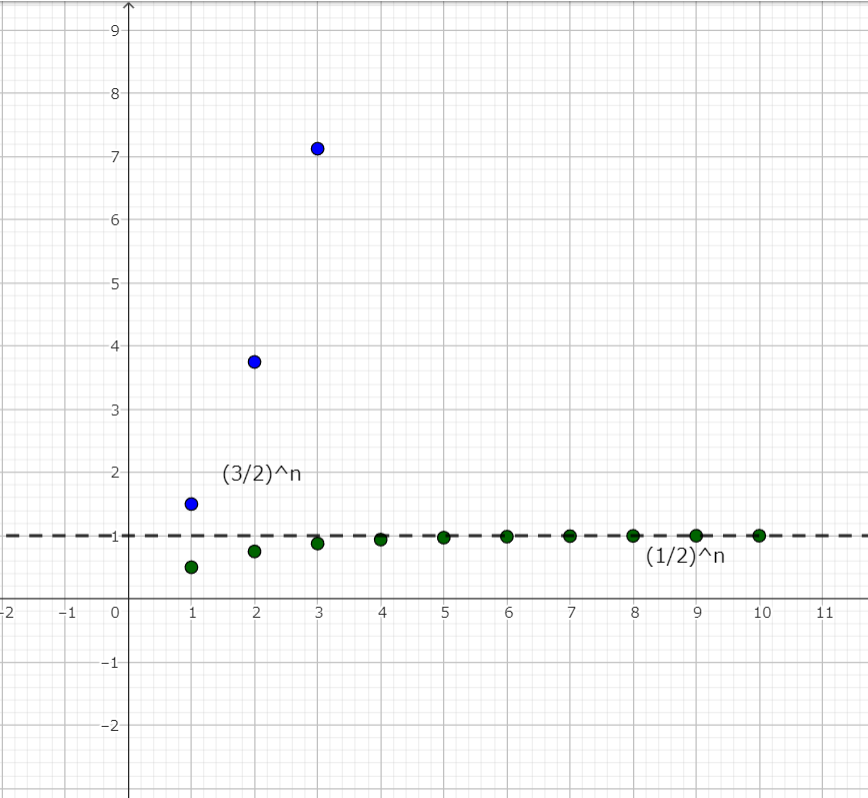
\includegraphics[scale=0.5]{img/QuuNote/seikoukyusu.png}
                    \caption{$n=10$までの部分和の比較}
                \end{figure}
            \clearpage
            \subsection{判定法}
                これから正項級数の収束・発散を判定する方法をいくつか述べる。

                \paragraph{比較法}正項級数$\sum a_n , \sum b_n$に対して、
                \begin{equation}
                    a_n \leq b_n \quad (n\geq N) \label{eq:比較法}
                \end{equation}
                であるとすれば、
                \begin{itemize}
                    \item $\sum b_n$が収束するとき、$\sum a_n$は収束する。
                    \item $\sum a_n$が発散するとき、$\sum b_n$は発散する。
                \end{itemize}
                これはよく考えたら当たり前のように感じる。証明もすごく簡単で、比較法の条件\eqref{eq:比較法}より、
                $n$が十分大きいとき$\sum^n a_n \leq \sum^n b_n$だから\footnote{$\sum^n a_n$は$a_n$の第$n$部分和を表すことにする。}、
                $\sum b_n$が収束するなら、ある定数$M$が存在して$\sum^n a_n \leq \sum^n b_n \leq M$となる。したがって$0\leq \sum^n a_n \leq M$となり、
                $\sum a_n$の$n$部分和も有界。よって$\sum a_n$も収束。さらに対偶を取れば$\sum a_n$が発散するとき$\sum b_n$も発散するとわかる。

                応用上は$N=1$として用いることが多い、また、級数の各項を定数倍しても級数の収束・発散は変わらないから、条件\eqref{eq:比較法}は$k>0$として
                $a_n \leq k b_n$としても、上記の判定法の結果は変わらない。

                これは最も基本的かつ有用な判定法である。以降の判定法もこの判定法から導出されるものが多い。この判定法は無意識に(わざわざ「比較法より」と書かずに)用いられる
                ことがよくある。\\

                \textbf{[例]}\hspace{1mm}$\displaystyle\sum \frac{1}{e^n + 1}$が収束するか調べる。明らかに$\displaystyle \frac{1}{e^n+1}\leq \frac{1}{e^n}$であり、$\sum e^{-n}$は収束するから
                $\displaystyle\sum \frac{1}{e^n+1}$も収束する。

                上の例からわかるように比較法の``キモ''はシグマの中の不等式評価をいかにうまくできるかにかかっている。例のような簡単な級数ならすぐ浮かぶが、中には
                技巧的な評価を行うもの(例えば調和数列など)もある。

                \paragraph{コーシーの判定法}正項級数$\sum a_n$において、
                \begin{equation}
                    \lim_{n\to \infty}\sqrt[n]{a_n} = L \label{eq:コーシーの判定法}
                \end{equation}
                とすると、
                \begin{itemize}
                    \item $0\leq L <1$ならば、$\sum a_n$は収束する。
                    \item $L>1$ならば、$\sum a_n$は発散する。
                \end{itemize}
                \paragraph{ダランベールの判定法}正項級数$\sum a_n$において、
                \begin{equation}
                    \lim_{n\to \infty}\frac{a_{n+1}}{a_n}=L\label{eq:ダランベールの判定法}
                \end{equation}
                とすると、
                \begin{itemize}
                    \item $0\leq L <1$ならば、$\sum a_n$は収束する。
                    \item $L>1$ならば、$\sum a_n$は発散する。
                \end{itemize}
                \clearpage
                コーシーの判定法もダランベールの判定法も、ともに等比級数と比較することで得られる。\sout{証明は}\\\sout{演習問題としよう。}\\

                \textbf{[例]}\hspace{1mm}$\displaystyle \sum_{n=0}^\infty \frac{x^n}{n!}$は$x$が有限な正の数であるとき収束することを示す。ダランベールの判定法を用いると
                \begin{equation*}
                    \lim_{n\to\infty}\frac{{x^{n+1}}/{(n+1)!}}{{x^n}/{n!}}=\lim_{n\to\infty}\frac{x}{n+1}=0
                \end{equation*}
                したがって、$L=0$より$\displaystyle\sum \frac{x^n}{n!}$は収束する。ちなみにこの級数の和は$e^x$である。\\

                どちらの判定法も\underline{$L=1$のときには何も言っていない(役に立たない)}ことに注意しよう。例を挙げるなら、
                $\sum 1/n^p$は、ダランベールの判定法を用いると
                \begin{equation*}
                    \lim_{n\to \infty}\frac{a_{n+1}}{a_n}=\lim_{n\to\infty}\frac{1/(n+1)^p}{1/n^p}=\lim_{n\to \infty}\frac{n^p}{(n+1)^p}=\lim_{n\to\infty}\frac{1}{\left(1+\frac{1}{n}\right)^p}=1
                \end{equation*}
                となり、$p$の値によらず$L=1$となってしまう。しかし実際には$p>1$なら収束し、$p\geq 1$なら発散するのである。

                \paragraph{積分判定法}正項級数を$\sum a_n$とする。このとき、関数$f(x)$を次のように選ぶ。$f$は$x\geq N$で$f>0$で、連続な広義減少
                関数であり、$x=N,N+1,N+2,\cdots$の点で、$a_{N},a_{N+1},a_{N+2},\cdots$を取るとする。すなわち
                \begin{equation*}
                    f(n)=a_n \quad (n=N,N+1,N+2,\cdots)
                \end{equation*}
                とする。このとき、無限積分
                \begin{equation*}
                    \int_{N}^{\infty}f(x)dx = \lim_{M\to\infty}\int_{N}^{M}f(x)dx \label{eq:積分判定法}
                \end{equation*}
                が収束すれば、正項級数$\sum a_n$は収束する。発散についても同様である。

                積分判定法のイメージにはグラフを書くことをお勧めする。級数の$n$部分和の図形的な意味も考えるとわかると思う。例えば、$N=1$で考えてみよう。$S_n=a_1+a_2+\cdots +a_n=1\times a_1 + 1\times a_2 +\cdots+1\times a_n$
                であるから、$S_n$は横の長さが1、縦の長さが$a_n$の各長方形の面積の和だと考えられる。$f$は広義の単調減少だから、これら長方形は各区間$[1,2],[2,3],\cdots,[n,n+1]$における各$f(x)$グラフ下の面積よりも大きい。
                すなわち
                \begin{equation*}
                    S_n \geq \int_1^{n+1} f(x)dx
                \end{equation*}
                である。また、各長方形の高さを$a_1\Rightarrow a_2,a_2\Rightarrow a_3,\cdots,a_{n}\Rightarrow a_{n+1}$とすれば、その面積の総和は
                $1\times a_{2}+1\times a_3+\cdots+1\times a_{n+1}=S_{n+1} - a_1$である。これらの各面積は$f$が広義単調減少だから、各$f(x)$のグラフ下の面積よりも小さい。
                すなわち
                \begin{equation*}
                    \int_{1}^{n+1}f(x)dx \geq S_{n+1}-a_1
                \end{equation*}
                である。
                \clearpage
                以上2つの不等式を合わせると、
                \begin{equation*}
                    S_n \geq \int_{1}^{n+1}f(x)dx \geq S_{n+1}-a_1
                \end{equation*}
                となるので、$n\to \infty$で積分が収束するかどうかが$S_n$が収束するかどうか、すなわち級数が収束するかどうかと同じだとわかるのである。\footnote{例えば$I_{n+1}=\int^{n+1}$を一つの数列と考えれば、この広義積分が収束するとき数列$I_n$は有界である。よって$\int^{n+1}\geq S_{n+1}-a_1$の不等式から、$S_n$も有界、つまり収束する。
                発散についても、$I_n$は広義単調増加するので考えられる発散の仕方は$I_n\to \infty$のみ。このとき不等式より$S_n \geq \infty$であるので、$S_n$は発散する。}

                積分判定法を用いれば、級数$\displaystyle \sum\frac{1}{n^p}$の収束・発散も調べられる。まず、$f$として$f(x)=1/x^p$を選べば、$f(n)=1/n^p =a_n \quad (n\geq 1)$となる。よって、
                積分$\displaystyle \int_{1}^{\infty}\frac{dx}{x^p}$が収束・発散の条件を調べればよい。積分の部の基本問題にあったように、$p>1$ならこの無限積分は収束し、$p\leq 1$なら発散する。
                したがって、級数$\displaystyle \sum \frac{1}{n^p}$は$p>1$ならば収束し、$p\leq 1$なら発散する。

                なお、$p>1$なる区間では級数の和は$p$の関数であるから、変数を$s$に変え、その関数を$\zeta(s)$とかく。これを\textbf{ゼータ関数}という。実は$s$は複素数まで
                拡張できる!実際、$\Re s > 1$であればゼータ関数は収束する。さらに解析接続\footnote{解析的延長とも。}という方法を用いればもっと広い範囲、例えば$\zeta(-1)$などまで
                関数を定義することができる。しかし、これは複素解析の話であり、このノートで扱う範囲を大きく超えているのでここでは扱わない。  
                
                \paragraph{名前がない判定法}上記の$\sum \frac{1}{n^p}$の性質と、比較法とを組み合わせると、次の判定法が得られる。この判定法は名前は私が知る限りでは無い。

                正項級数$\sum a_n$に対して、
                \begin{equation}
                    \lim_{n\to\infty}n^p a_n = A \label{eq:名もなき判定法}
                \end{equation}
                を計算する。
                \begin{itemize}
                    \item $p>1$で$A$が有限ならば、$\sum a_n$は収束する。
                    \item $p\leq 1$で$A\neq 0$(無限大も含めて)なら、$\sum a_n$は発散する。
                \end{itemize}
                ちなみにこの判定法に限らず、たいていの判定法を導出するにはコーシーの収束判定法\footnote{これは数列に関するコーシーの収束定理から導ける。}という方法を用いるが、このノートでは扱わないので証明を載せることはできない。\\

                \textbf{[例]}\hspace{1mm}$\sum \sin^2(\frac{1}{n})$の収束を調べる。十分大きい$n$について$\sin \frac{1}{n} = \frac{1}{n}$が成り立つ\footnote{イメージは$x\to 0$で$\sin x/x\to 1$であることから。}ので、$p=2$として
                $\lim n^2\cdot\frac{1}{n^2}=\lim 1=1=A.$したがって、$A$は有限なので級数は収束する。

                \paragraph{ラーベの判定法}正項級数を$\sum a_n$とすると、
                \begin{equation}
                    \lim_{n\to\infty}n\left(\frac{a_n}{a_{n+1}}-1\right)=r \label{eq:ラーベの判定法}
                \end{equation}
                このとき、$r>1$ならば収束し、$r<1$ならば発散する。
            \clearpage
            \subsection{交項級数}
                これまでは、級数の各項の符号が同じ場合についてのみ扱った。ここからは符号が一定でない場合の級数も含めて扱っていく。

                まず、符号が交互に代わる級数(\textbf{交項級数})を考えよう。これは各項が負ではない数列$\left\{b_n\right\}$を用いて
                \begin{equation}
                    b_1-b_2+b_3-b_4+\cdots
                \end{equation}
                と表せられる。交項級数は以下の条件が満たされるときに収束する。
                \begin{enumerate}
                    \item $0\leq b_{n+1}\leq b_n$
                    \item $\lim b_n = 0$
                \end{enumerate}
                上記の条件が満たされていると仮定して収束することを示す。この時、最初の$2M$項の和は
                \begin{equation}
                    S_{2M}=(b_1-b_2)+(b_3-b_4)+(b_5-b_6)+\cdots +(b_{2M-1}-b_{2M})\label{eq:交項級数証明用1}
                \end{equation}
                また、
                \begin{equation}
                    S_{2M}=b_1-(b_2-b_3)-(b_4-b_5)-\cdots - (b_{2M-2}-b_{2M_1})-b_{2M}\label{eq:交項級数証明用2}
                \end{equation}
                式\eqref{eq:交項級数証明用1}では、すべての(\hspace{2mm})が負ではない。したがって、
                \begin{equation}
                    S_{2M}\geq 0,\quad S_2\leq S_4\leq\cdots\leq S_{2M}
                \end{equation}
                また、式\eqref{eq:交項級数証明用2}でも、(\hspace{2mm})内の量はすべて負ではないし、$b_{2M}\geq 0$であるから、$S_{2M}\leq b_1$である。
                したがって、
                \begin{equation}
                    0\leq S_2\leq S_4\leq\cdots\leq S_{2M}\leq b_1
                \end{equation}
                すなわち、$\left\{S_{2M}\right\}$は広義単調減少で有界であるから、収束し、極限値$S$を持つ。

                さらに、$S_{2M+1}=S_{2M}+b_{2M+1}$であるから、$\lim b_{2M+1}=0$より
                \begin{equation*}
                    \lim_{n\to\infty}S_{2M+1}=\lim_{n\to\infty}\left\{S_{2M}+b_{2M+1}\right\}=S+0=S
                \end{equation*}
                よって、この級数の第$n$部分和$S_n$は、$n$が偶数でも奇数でも極限値$S$を持ち、収束する。

                \paragraph{例}$\displaystyle\sum (-1)^{n+1}\frac{1}{n}$は収束する。なぜなら、$\displaystyle 0\leq \frac{1}{n+1}\leq \frac{1}{n}$であり、$\displaystyle\lim_{n\to \infty}\frac{1}{n}=0$
                であるから、交項級数の収束条件が満たされる。
            \clearpage
            \subsection{絶対収束級数}
                今度は符号の制限をなくし、任意の符号を持つ数列$\{a_n\}$からつくられる級数
                \begin{equation*}
                    \sum a_n = a_1+a_2+a_3+\cdots+a_n+\cdots \label{eq:絶対収束用級数}
                \end{equation*}
                を考えよう。この級数の各項の絶対値を取った
                \begin{equation*}
                    \sum |a_n| = |a_1|+|a_2|+|a_3|+\cdots+|a_n|+\cdots\label{eq:絶対収束用級数_絶対値}
                \end{equation*}
                は正項級数である。

                このとき、級数\eqref{eq:絶対収束用級数_絶対値}が収束するならば、級数\eqref{eq:絶対収束用級数}は\textbf{絶対収束する}といい、
                このような級数を\textbf{絶対収束級数}という。

                それぞれの級数の第$n$部分和を
                \begin{equation*}
                    S_n = \sum_{k=1}^{n}a_k,\quad T_n = \sum_{k=1}^{n}|a_k|
                \end{equation*}
                と置けば、
                \begin{equation*}
                    S_n+T_n=(a_1+|a_1|)+(a_2+|a_2|)+\cdots+(a_n+|a_n|)\leq 2(|a_1|+|a_2|+\cdots+|a_n|)
                \end{equation*}
                である。ここで$\sum a_n$が絶対収束するとすれば、$a_n+|a_n|\leq 0$であることを併せて、$S_n+T_n$は
                有界な広義の単調増加数列となる。すなわち、$\lim (S_n+T_n)$は収束する。よって、$\lim S_n$も収束する。
                つまり、絶対収束級数は``絶対に''収束するのである。名前負けしてないのが面白い。

                逆に、$\sum a_n$は収束するが、$\sum|a_n|$が発散するとき、$\sum a_n$は\textbf{条件収束する}という。
                またこの級数を\textbf{条件収束級数}という。\\

                以前正項級数の判定法を述べたが、これは絶対収束の判定にも使うことができる。むしろ、絶対収束の判定のために
                これまでの判定法を述べたのである、というのは過言か。

                \paragraph{例}級数
                \begin{equation*}
                    \sum_{n=0}^{\infty}\frac{x^n}{n!}
                \end{equation*}
                は、すべての有限な$x$に対して絶対収束する。なぜなら、ダランベールの判定法を用いると、
                \begin{equation*}
                    \lim_{n\to \infty}\frac{{|x^{n+1}|}/{(n+1)!}}{{|x^n|}/{n!}}=\lim_{n\to\infty}\frac{|x|}{n+1}=0
                \end{equation*}
                よって、この級数は絶対収束し、収束する。
            \clearpage
            \basicquestion 以下の問いに答えよ。
                \paragraph{問1}比較法を用いて、次の級数の収束、発散を調べよ。\\
                $\displaystyle(1)\sum_{n=2}^{\infty}\frac{1}{\log n}$\hspace{15mm}
                $\displaystyle(2)\sum_{n=1}^{\infty}\frac{\log n}{n^3+1}$\hspace{15mm}
                $\displaystyle(3)\sum_{n=1}^{\infty}\frac{n^2+1}{n^3+1}$

                \paragraph{問2}コーシーの判定法かダランベールの判定法を用いて、次の級数の収束、発散を調べよ。\\
                $\displaystyle(1)\sum_{n=1}^{\infty}\frac{1}{n^n}$\hspace{15mm}
                $\displaystyle(2)\sum_{n=1}^{\infty}n^5e^{-n^2}$\hspace{15mm}
                $\displaystyle(3)\sum_{n=1}^{\infty}\left(\frac{n}{2n+1}\right)^n$

                \paragraph{問3}積分判定法より、次の級数の収束、発散を調べよ。\\
                $\displaystyle(1)\sum_{n=1}^{\infty}\frac{n}{n^2+2}$\hspace{15mm}
                $\displaystyle(2)\sum_{n=1}^{\infty}ne^{-n^2}$\hspace{15mm}
                $\displaystyle(3)\sum_{n=2}^{\infty}\frac{1}{n\log n}$

                \paragraph{問4}$\lim n^p a_n$を計算することで、次の級数の収束、発散を調べよ。\\
                $\displaystyle(1)\sum_{n=1}^{\infty}\frac{n}{3n^3-1}$\hspace{15mm}
                $\displaystyle(2)\sum_{n=1}^{\infty}\frac{\log n}{\sqrt{n+2}}$\hspace{15mm}
                $\displaystyle(3)\sum_{n=1}^{\infty}\sin^3\left(\frac{1}{n}\right)$

                \paragraph{問5}次の級数の収束、絶対収束を調べよ。\\
                $\displaystyle(1)\sum_{n=1}^{\infty}\frac{(-1)^{n-1}}{n^2}$\hspace{15mm}
                $\displaystyle(2)\sum_{n=1}^{\infty}(-1)^{n-1}\frac{\log n}{n^3+1}$\hspace{15mm}
                $\displaystyle(3)\sum_{n=1}^{\infty}\frac{(-1)^{n-1}}{n}$
                
                \paragraph{問6}次の収束・発散を調べよ。\\
                $\displaystyle (1)\sum_{n=1}^{\infty}\frac{(a+1)(2a+1)\cdots(na+1)}{(b+1)(2b+1)\cdots(nb+1)}\quad (a,b>0)$\\
                $\displaystyle (2)\sum_{n=2}^{\infty}(-1)^n\frac{\log n}{n}$\\
                $\displaystyle (3)\sum_{n=1}^{\infty}\frac{(a+1)(a+2)\cdots(a+n)}{(b+1)(b+2)\cdots(b+n)}\quad (a,b>0)$

                \paragraph{問7}条件$0\leq b_{n+1} \leq b_n,\lim b_n =0$を満たす交項級数$b_1-b_2+b_3-\cdots$において、ある項までで打ち切ることによる
                誤差は、次の項の絶対値より小さい。これを示せ。ただし、誤差とは級数をある項までで打ち切った時の和と級数の和との差の絶対値とする。
            \clearpage
        \section{関数級数}
            いよいよ最後の節となった。ここでは関数列からなる級数である関数級数について、一様収束という概念と絡めて述べていく。
            \subsection{一様収束}
                一般に、\textbf{関数列}$\{u_n(x)\}=u_1(x),u_2(x),\dots$から作られる級数を\textbf{関数級数}という。
                \begin{equation}
                    \sum_{n=1}^{\infty}u_n=u_1(x)+u_2(x)+\cdots\label{eq:関数級数}
                \end{equation}
                例えば、フーリエ級数やべき級数がある。フーリエ級数はフーリエ解析で特別詳しく扱うだろうからここでは深く述べない。その代わり、べき級数について後になって扱う。
 
                さて、関数級数\eqref{eq:関数級数}の第$n$部分和を$f_n(x)$で表すことにすれば、
                \begin{equation}
                    f_n(x)=u_1(x)+u_2(x)+\cdots+u_n(x)\label{eq:関数級数のn部分和}
                \end{equation}
                である。この時、任意の正数$\varepsilon>0$に対して、\underline{$x$に関係ない}数$N$が存在して、$n\geq N$のすべての$n$に対して
                \begin{equation}
                    |f(x)-f_n(x)|<\varepsilon\quad (n\geq N)\label{eq:一様収束}
                \end{equation}
                が成り立つならば、この級数は\textbf{一様収束}するという。そして、$f(x)$を\textbf{関数級数の和}という。下線部のところの条件が重要で、
                この時$N=N(\varepsilon)$であり、$N=N(\varepsilon,x)$であってはいけないのである。\footnote{逆に、$x$にも依存して$f$が決まる場合は\textbf{各点収束する}という。}

                一様収束と収束の違いはどのようなものだろうか。たとえば簡単なものとして、$f_n(x) = e^{-nx}$を$0\leq x< \infty$考えてみよう。この時$n\to \infty$の極限でこの級数は収束して、
                \begin{equation*}
                    \lim_{n\to\infty}f_n(x)=\begin{cases}
                        1\quad &(x=0)\\0\quad &(x>0)
                    \end{cases}
                \end{equation*}
                である。しかし、一様収束はしない。なぜなら、$x>0$のとき、$1>e^{-nx}$であるから、
                \begin{equation*}
                    |f(x)-f_n(x)|=|1-e^{-nx}|=1-e^{-nx}<\varepsilon\quad (\varepsilon < 1)
                \end{equation*}
                となればよいが、そのためには
                \begin{equation*}
                    N=\left\lfloor\frac{1}{x}\log\left(\frac{1}{1-\varepsilon}\right)\right\rfloor+1
                \end{equation*}
                と$N$を取らなければならない。ここで、ガウス記号\footnote{実数$x$に対して整数$n$が$n\leq x<n+1$であるとき、$n=\lfloor x\rfloor$と表す。}を用いた。$N$は$x$が$0$に近づくにつれて大きくとらなければならない。すなわち、
                $N$は$\varepsilon$だけでなく$x$にも依存してしまっているのである。
            \clearpage
            \subsection{一様収束の性質}
                ここからは、関数級数が一様収束すると何がうれしいのかについて述べる。まず、区間$a\leq x\leq b$で$\{u_n(x)\}$の各項が連続であるとしよう。この時、この関数列から作られる級数
                \begin{equation*}
                    \sum_{n=1}^{\infty}u_n(x)=u_1(x)+u_2(x)+u_3(x)+\cdots
                \end{equation*}
                を考えるとしよう。また、第$n$項までの和を
                \begin{equation*}
                    f_n(x)=u_1(x)+u_2(x)+u_3(x)+\cdots +u_n(x)
                \end{equation*}
                と置く。

                \paragraph{連続性}連続関数級数$\sum u_n(x)$が和$f(x)$に一様収束するなら、$f(x)$は連続な関数である。言い換えると、一様収束するなら$f_n(x)$の連続性は$f(x)$に遺伝する。

                これを一様収束の定義から導出してみよう。まず、$x$と$x+h$が区間$[a,b]$内にあるとする。このとき、
                \begin{align*}
                    |f(x+h)-f(x)|&=|f(x+h)-f_n(x+h)+f_n(x+h)-f_n(x)+f_n(x)-f(x)|\\ &\leq |f(x+h)-f_n(x+h)|+|f_n(x+h)-f_n(x)|+|f_n(x)-f(x)|
                \end{align*}
                である。まず、$f_n$が一様収束するのだから、$n$を十分大きくとると
                \begin{equation*}
                    |f(x+h)-f_n(x+h)|<\frac{\varepsilon}{3},\quad |f(x)-f_n(x)|<\frac{\varepsilon}{3}
                \end{equation*}
                とできる。さらに、$f_n$は連続であるから、
                \begin{equation*}
                    |f_n(x+h)-f_n(x)|<\frac{\varepsilon}{3}\quad (|h|<\delta)
                \end{equation*}
                となるように$\delta$を取ることができる。\footnote{なぜなら、十分大きく$n$を取っているので、その値を$N_0(\frac{\varepsilon}{3})$とすれば、$f_{N_0(\frac{\varepsilon}{3})}$は連続なので、ある$\delta_{N_0(\frac{\varepsilon}{3})}$が存在するはずである。ここでは関数列$\{f_n(x)\}$の中から一つ関数を取ってくるのがポイントである。そうしないとそれぞれの$n$に対して$\delta_n$が存在してしまうため、例えば$\delta=\delta_n$と選ぼうとすると、$n$に依存してしまうのである。}
                よって、
                \begin{equation*}
                    |f(x+h)-f(x)|<\varepsilon \quad (|h|<\delta)
                \end{equation*}
                が成り立つので、$f(x)$は連続である。

                この定理の対偶を取れば、次の事実が得られる。それは、和$f(x)$がある点で不連続ならば、級数$\sum u_n(x)$はその点を含む区間で一様収束しない。

                例えば、$f_n(x)=e^{-nx}$は、$f(x)$が$x=0$で不連続であるため、区間$[0,\infty)$で一様収束しない。
                \clearpage
                \paragraph{項別積分}連続関数級数$\sum u_n(x)$が和$f(x)$に一様収束すれば、
                \begin{equation}
                    \sum_{n=1}^{\infty}\int_{a}^{b}u_n(x)dx = \int_a^b f(x)dx \label{eq:項別積分}
                \end{equation}
                すなわち、一様収束すれば級数は項別に積分できる。

                これも、一様収束の定義から導出できる。まず、部分和$f_n(x)$と和$f(x)$は$a\leq x\leq b$で連続だから積分できる。
                したがって、任意の$\varepsilon>0$に対し、$x$と無関係な$N$が存在して、$n\geq N$なら、
                \begin{equation*}
                    \left|\int_{a}^{b}f_n(x)dx -\int_a^b f(x)dx\right|=\left|\int_{a}^{b}f_n(x)-f(x)dx\right|\leq \int_{a}^{b}|f_n(x)-f(x)|dx<\int_{a}^{b}\varepsilon dx=\varepsilon(b-a)
                \end{equation*}
                とできる。ここで、積分$\int_{a}^{b}f_ndx$を数列と見れば、
                \begin{equation*}
                    \lim_{n\to\infty}\int_{a}^{b}f_n(x)dx = \int_{a}^{b}f(x)dx=\int_{a}^{b}\lim_{n\to \infty}f_n(x)dx
                \end{equation*}
                を意味する。すなわち、\eqref{eq:項別積分}が示された。

                これは、一様収束する関数列は\underline{積分と極限が交換できる}ことを示している。この性質は非常に重要で、安易に積分記号と極限を入れ替えてはいけないことを思い出させてくれる。

                \paragraph{項別微分}連続関数級数$\sum u_n(x)$が和$f(x)$に一様収束\footnote{実はこの時$\{f_n\}$が一様収束ではなく、各点収束でもこれは成り立つ。}し、導関数から作られた連続関数級数$\sum u_n'(x)$が和$g(x)$に一様収束すれば、
                \begin{equation}
                    \frac{d}{dx}f(x)=g(x) \Leftrightarrow \frac{d}{dx}\sum_{n=1}^{\infty}u_n(x)=\sum_{n=1}^{\infty}\frac{d}{dx}u_n(x) \label{eq:項別微分}
                \end{equation}
                すなわち、級数$\sum u_n(x)$は項別微分ができる。

                もちろんこれも一様収束の定義から導出できる。ということで示していく。まず、$g(x)=\sum u_n'(x)$は一様収束するから、項別に積分ができて、
                \begin{equation*}
                    \int_{a}^{x}g(x)dx = \sum_{n=1}^{\infty}\int_{a}^{x}u_n'(x)dx = \sum_{n=1}^{\infty}\left\{u_n(x)-u_n(a)\right\}=f(x)-f(a)
                \end{equation*}
                よって、両辺を$x$微分すれば、式\eqref{eq:項別微分}を得る。

                これは、部分和$f_n(x)=u_1(x)+u_2(x)+\cdots+u_n(x)$が作る関数列に対して、微分と極限が交換できることを示している。
                \begin{equation*}
                    \frac{d}{dx}\lim_{n\to\infty}f_n(x)=\lim_{n\to\infty}\frac{d}{dx}f(x)
                \end{equation*}\\

                上記の結果をまとめると、一様収束する連続関数級数は連続であり、項別に微分積分できる。これは、有限個の項の和$u_1(x)+u_2(x)+\cdots+u_n(x)$
                が持つ性質が成り立つということである。一様収束が持つ性質のよさがわかってもらえただろうか。正直一様収束性をいちいち気にして極限と積分を入れ替える
                なんて面倒なことをしたくないものだが、厳密な論理のためにはこれは必要なのである。
            \clearpage
            \subsection{べき級数}
                ついに最後の項に入る。ここではべき級数(巾級数)について述べる。べき級数は解析学で最も重要な級数であり、これを用いれば、関数の性質を調べたり近似したり、より広い範囲の関数を扱えるようになる。
                べき級数がなぜ大事かについては最後にまとめて述べることにして、まずはその性質を調べていこう。\\

                まず、$a_0,a_1,a_2,a_3\cdots$を定数として、無限級数
                \begin{equation}
                    \sum_{n=0}^{\infty}a_n x^n =a_0+a_1x+a_2x^2+a_3x^3+\cdots\label{eq:べき級数}
                \end{equation}
                を$x$の\textbf{べき級数}という。本によっては整級数と書くこともある。また、
                \begin{equation}
                    \sum_{n=0}^{\infty}a_n (x-a)^n =a_0+a_1(x-a)+a_2(x-a)^2+a_3(x-a)^3+\cdots
                \end{equation}
                を$x-a$のべき級数という。これは式\eqref{eq:べき級数}で$x=(x-a)$としたものだから以降は$\sum a_nx^n$の形で扱う。

                さて、べき級数の収束について基本的なことを述べよう。
                \begin{itembox}{アーベルの定理(?)}
                    もしべき級数$\sum a_nx^n$が$x=x_0$のときに収束すれば、$|x|<|x_0|$であるすべての$x$の値に関して絶対収束し、領域$|x|<|x_0|$に含まれる
                    任意の閉区域において一様に収束する。
                \end{itembox}
                まずはこれを証明しておく。まず、$|x|<|x_0|$である$x$をもちいて、べき級数を次のように変形する。
                \begin{equation*}
                    \sum a_nx^n = \sum a_n x_0^n\cdot\left(\frac{x}{x_0}\right)^n
                \end{equation*}
                ダランベールの判定法から
                \begin{equation*}
                    L=\lim \left|\frac{a_{n+1}x_0^{n+1}\cdot \left(\frac{x}{x_0}\right)^{n+1}}{a_{n}x_0^{n}\cdot\left(\frac{x}{x_0}\right)^{n}}\right|=\lim\left|\frac{a_{n+1}x_0^{n+1}}{a_{n}x_0^{n}}\right|\cdot \lim\left|\frac{\left(\frac{x}{x_0}\right)^{n+1}}{ \left(\frac{x}{x_0}\right)^{n}}\right|=\lim\left|\frac{a_{n+1}x_0^{n+1}}{a_{n}x_0^{n}}\right|\cdot \left|\frac{x}{x_0}\right|
                \end{equation*}
                ここで、$x_0$の点においてべき級数が収束すると仮定すれば、最後の極限値$L_0$は$0\leq L_0<1$である。条件から$\left|\frac{x}{x_0}\right|<1$であるから、$0\leq L<1$、すなわち級数は収束する。よって$|x|<|x_0|$である$x$について級数は絶対収束する。また、$\sum a_nx_0^n$は収束するのだから、十分大きな$n$に対しては$|a_nx_0^n| < \varepsilon$とできる。
                すなわち、
                \begin{equation*}
                    \left|\sum_{k}^\infty a_kx^k - \sum_k^{\text{十分大きな}n}a_kx^k\right|=\left|\sum_{k=n+1}a_kx^{k}\right|\leq \sum_{n}|a_kx^k|=\sum_{n}|a_kx_0^k\cdot \frac{x^k}{x_0^k}|<\varepsilon\sum_{n}\left|\frac{x}{x_0}\right|^k=\varepsilon\cdot \frac{\left|\frac{x}{x_0}\right|^n}{1-\left|\frac{x}{x_0}\right|}
                \end{equation*}
                とできる。最後の等式は級数を最初の変形のように分けて実際に計算することで得られる。ここで、先ほども述べたように$\left|\frac{x}{x_0}\right|<1$であるから
                \begin{equation*}
                    \left|\sum_{k}^\infty a_kx^k - \sum_k^{\text{十分大きな}n}a_kx^k\right|<\frac{\varepsilon}{1-\left|\frac{x}{x_0}\right|}
                \end{equation*}
                $\varepsilon$は任意であるから、結局$n$を十分大きくすれば、($x$の値に関係なく)$|\sum^{\infty}-\sum^{n}|$をいくらでも小さくできる。すなわち、べき級数$\sum a_nx^n$は$|x|<|x_0|$に含まれる任意の兵区域において一様に収束する。$\square$


                もし、$x=x_0$で発散すれば、そのべき級数は$|x|>|x_0|$であるすべての$x$に対して発散する。なぜなら、仮にある$|x_1|>|x_0|$である点$x=x_1$で収束するとすれば、当然$x=x_0$も収束することになるため、仮定に反してしまう。

                以上をまとめると、べき級数を収束せしめる$|x|$の値には上限があることがわかる。これを$r$と置けば、べき級数は$|x|<r$であるとき、
                すなわち原点中心半径$r$の円の内側にあるときに収束し、円の外側にあるときに発散する。このような円をべき級数の収束円といい、その半径$r$を\textbf{収束半径}という。
                いまは$x$の範囲が一次元的(x軸)であるため、円のイメージを持ちにくいが、$x$を複素数$z=x+iy$に拡張すれば、$z$の範囲は二次元的(実軸と虚軸)になるので、自然な命名であるように感じる。
                もっとも、それは複素解析の範囲であるのでここでは扱わないが。

                なお、べき級数が任意の$x$に対して収束するなら$r=\infty$とし、$x=0$以外では収束しないときは$r=0$とする。例えば、$\sum x^n$の収束半径は$r=1$である。また、$\sum x^n/n!$は$r=\infty$である。
                \clearpage
                収束半径$r$は、ダランベールの判定法とコーシーの判定法を用いれば、以下の公式で求められる。
                \begin{equation}
                    r=\lim_{n\to\infty}\left|\frac{a_n}{a_{n+1}}\right|\label{eq:ダランベールの判定法と収束半径}
                \end{equation}
                \begin{equation}
                    \frac{1}{r}=\lim_{n\to\infty}\sqrt[n]{|a_n|}\label{eq:コーシーの判定法と収束半径}
                \end{equation}

                \paragraph{例}べき級数$\displaystyle\sum_{n=1}^\infty(-1)^{n-1}\frac{x^n}{n}$が収束する$x$の範囲を求める。公式\eqref{eq:ダランベールの判定法と収束半径}を用いると、
                \begin{equation*}
                    r=\lim_{n\to\infty}\left|\frac{(-1)^{n-1}\frac{1}{n}}{(-1)^n\frac{1}{n+1}}\right|=\lim_{n\to\infty}\left|\frac{n+1}{n}\right|=1
                \end{equation*}
                よって、$|x|<1$では収束する。$|x|=1$では、まず$x=1$のとき、級数$\sum (-1)^{n-1}\frac{1}{n}$は収束する。一方$x=-1$のとき、級数$\sum \frac{1}{n}$は収束しない。
                まとめると、収束する範囲は$-1<x\leq 1$である。

                上の例からわかるように、$|x|=r$のときは個別に収束するかどうか調べなければならない。つまり、区間の端点$x=r,x=-r$のときを調べればよい。\\

                先ほどの定理でも述べたように、べき級数は$|x|<r$で一様収束する。すなわち、以下の性質が成り立つ。
                \begin{enumerate}
                    \item[\textbf{連続性}] 開区間$|x|<r$で連続な関数を表す。
                        \begin{equation}
                            f(x)=\sum_{n=0}^{\infty}a_nx^n = a_0+a_1x+a_2x^2+\cdots
                        \end{equation}
                    \item[\textbf{項別積分}] 開区間$|x|<r$の任意の点において、項別積分が可能で、得られたべき級数$\sum a_n x^{n+1}/(n+1)$は同じ収束半径$r$をもち、その級数の和は$f(x)$を積分したものと等しい。
                        \begin{equation}
                            \int_{0}^{x}f(x)dx=\sum_{n=0}^{\infty}\frac{a_n}{n+1}x^{n+1}
                        \end{equation}
                    \item[\textbf{項別微分}] 開区間$|x|<r$の任意の点において、項別積分が可能で、得られたべき級数$\sum a_n nx^{n-1}$は同じ収束半径$r$をもち、その級数の和は$f(x)$を微分したものと等しい。 
                        \begin{equation}
                            \frac{d}{dx}f(x)=\sum_{n=1}^{\infty}nc_{n}x^{n-1}
                        \end{equation}
                \end{enumerate}

                項別微分の性質から、収束半径$r$を持つべき級数は何回でも項別微分可能で、収束半径はすべておなじ$r$であることがわかる。もちろん項別積分についても同様のことが言える。
                このことから、関数をべき級数表示してみよう。まず、収束半径を$r$として、
                \begin{equation*}
                    f(x)=c_0+c_1x+c_2c^2+\cdots\quad (|x|<r)
                \end{equation*}
                であるとしよう。この時、項別微分を次々に行うと、
                \begin{align*}
                    f'(x)&=c_1+2c_2x+3c_3x^2+\cdot\\
                    f''(x)&=2c_2+3\cdot 2 c_3x+4\cdot 3c_{4}x^2\\
                    &\cdots\cdots\\
                    f^{(n)}(x)&=n!c_n+(n+1)n\cdots3\cdot2c_{n+1}x+\cdots
                \end{align*}
                である。ここで、$x=0$を代入すれば、
                \begin{equation*}
                    c_0=f(0),\quad c_1=f'(0),\quad 2c_2=f''(0),\cdots,n!c_n = f^{(n)}(0),\cdots
                \end{equation*}
                が得られる。すなわち、
                \begin{equation}
                    f(x)=f(0)+\frac{f'(0)}{1!}x+\frac{f''(0)}{2!}x^2+\cdots+\frac{f^{(n)}(0)}{n!}x^n+\cdots\quad(|x|<r)\label{eq:マクローリン級数}
                \end{equation}
                が得られる。この級数は$f(x)$をマクローリン展開したものと同じであるので、\textbf{マクローリン級数}という。

                同様に、$|x-a|<r$で収束するべき級数に対しても、
                \begin{equation}
                    f(x)=f(a)+\frac{f'(a)}{1!}(x-a)+\frac{f''(a)}{2!}(x-a)^2+\cdots+\frac{f^{(n)}(a)}{n!}(x-a)^n+\cdots\quad(|x-a|<r)\label{eq:テイラー級数}
                \end{equation}
                が成り立つ。これを\textbf{テイラー級数}という。\eqref{eq:マクローリン級数}も合わせてテイラー級数ということもある。

                以下に主な関数のマクローリン展開を上げよう。
                \begin{align}
                    \frac{1}{x+1}&=\sum_{n=0}^{\infty}(-1)^nx^n \quad &&(-1<x<1)\label{eq:1/x+1のマクローリン級数}\\
                    e^x &= \sum_{n=0}^{\infty}\frac{x^n}{n!} &&(-\infty<x<\infty)\label{eq:expのマクローリン級数}\\
                    \sin x &= \sum_{n=0}^{\infty}(-1)^n\frac{x^{2n+1}}{(2n+1)!} &&(-\infty<x<\infty)\label{eq:sin xのマクローリン級数}\\
                    \cos x &= \sum_{n=0}^{\infty}(-1)^n\frac{x^{2n}}{(2n)!} &&(-\infty<x<\infty)\label{eq:cos xのマクローリン級数}\\
                    \log(x+1) &= \sum_{n=0}^{\infty}(-1)^n\frac{x^{n+1}}{(n+1)} &&(-1<x\leq 1)\label{eq:log x+1のマクローリン級数}
                \end{align}
                最後の収束範囲について気を付けなければならない。これに限らず、(基本的には)公式はまず適用条件を確かめる必要がある。

                以前も述べたように、べき級数は$x$を複素数$z$まで拡張して定義することができる。そして、複素数に拡張したとしても上式\eqref{eq:expのマクローリン級数},\eqref{eq:sin xのマクローリン級数},\eqref{eq:cos xのマクローリン級数}
                の収束半径は$r=\infty$のままである。よって、$e^x$に$x=i\theta$を入れれば、
                \begin{equation}
                    e^{i\theta}=\cos\theta + i\sin\theta
                \end{equation}
                が導ける。つまり、三角関数が(複素)指数関数に含まれてしまうのである!これを\textbf{オイラーの公式}という。

                最後に、べき級数がなぜ大事なのかについて少しだけだが述べよう。まずはやはり関数の近似が行える点だろう。これにはテイラー級数やマクローリン級数を用いればよい。
                次に、初等関数で表せない関数だとしても、べき級数で書けば情報を得ることができる。例えば、不定積分
                \begin{equation*}
                    f(x)=\int_{0}^{x}e^{-x^2}dx
                \end{equation*}
                は初等関数で表せないが、被積分関数をべき級数で表し、項別積分すれば、有用な表式が得られる。さらに、べき級数は収束範囲内の$x$に対して一つの値$y$を与える。
                これにより、より広い範囲の関数を扱う対象とできるようになる。
                \clearpage
            \subsection{補足}
                重要であるが、本文の流れを損なわないために書けなかったこと等について軽くまとめておく。
                \begin{itembox}{アーベルの連続定理}
                    べき級数$f(z)=\sum a_nz^n$が収束円の円周上の点$z=\zeta$において収束すれば、$z$が半径に沿って$\zeta$に近づくとき
                    \begin{equation}
                        \lim_{z\to\zeta}f(z)=\sum_{n=0}^{\infty}a_n\zeta^n
                    \end{equation}
                \end{itembox}
                これは自明ではない。なぜなら、上記等式は
                \begin{equation*}
                    \lim_{z\to\zeta}\left(\lim_{n\to\infty}\sum_{k=0}^{n}a_kz^{k}\right)=\lim_{n\to\infty}\left(\lim_{z\to\zeta}\sum_{k=0}^{n}a_kz^{k}\right)
                \end{equation*}
                を意味するが、極限$\lim$を無頓着に入れ替えてはいけないことはよくわかっていることだろう。つまりこの定理の意味とは、右辺の極限が確定ならば、$\lim$の入れ替えが可能であるというのである。
                なお、これは複素数まで拡張した場合のべき級数で、これを実数版に直すなら、例えば$r=1$のときは、
                \begin{equation*}
                    \lim_{x\to 1-0}f(x)=f(1)
                \end{equation*}
                である。\\

                \begin{itembox}{フーリエ級数展開}
                    区間$[-\pi,\pi]$において与えられた関数$f(x)$は\underline{或る条件}のもとにおいて、次の三角級数に展開される。
                    \begin{equation}
                        f(x)=\frac{a_0}{2}+\sum_{n=1}^{\infty}\left\{a_n\cos(nx)+b_n\sin(nx)\right\}\label{eq:フーリエ級数}
                    \end{equation}
                    このような級数を$f(x)$のフーリエ級数(フーリエ級数展開)という。もし、このような展開が可能であるとして、$f$が積分可能で、さらに級数に項別積分ができるとすれば、$a_n,b_n$は確定して、
                    \begin{equation*}
                        a_n=\frac{1}{\pi}\int_{-\pi}^{\pi}f(x)\cos(nx)dx,\quad b_n=\frac{1}{\pi}\int_{-\pi}^{\pi}f(x)\sin xdx
                    \end{equation*}
                    である。ただし、$a_n$において$n=0,1,2,\cdots$であり$b_n$において$n=1,2,\cdots$である。
                \end{itembox}
                すこしだけフーリエ解析の内容を入れてみた。これがフーリエ級数展開できる条件を導くのは今の状態ではとても難しいので省略する。\footnote{むしろ証明を補足でしたらそれは果たして補足といえるのだろうか?}例えば高木貞二の解析概論を参照。

                とはいえ、いきなりこの式を丸暗記するというのも難しい話である。そこで以下で、フーリエ級数の各係数$a_n,b_n$がどのようにして上記のように与えられているかを簡単に追ってみようと思う。説明を簡単にするために厳密な説明等がなされていない場合があるが大目に見てほしい。

                まず、$0$ではない有限個または無限この関数の集まりを関数系と呼ぶと呼ぶことにする。ここでいう$0$ではないの意味は、$f(x)=0$となる$x$が存在しないという意味ではなく、どんな$x$に対しても$f(x)=0$である関数ではないという意味である。すなわち、恒等的に$0$ではない関数という意味である。さて、その関数系のすべての関数$\phi_n(x)$が
                ある変域において定義され、$|\phi_n(x)|,[\phi_n(x)]^2$がその辺域内の任意の区間において積分可能だとする。

                一般に
                \begin{equation*}
                    C_0\phi_0+C_1\phi_1+C_2\phi_2+\cdots+C_n\phi_n = 0
                \end{equation*}
                が、定数$C_0=C_1=C_2=\cdots=C_n=0$のときのみ成立するとき、上記の関数系を\textbf{線形独立}な関数系といい、そうでなければ線形従属な関数系という。ここあたりは線形代数と同じで特別難しくないだろう。

                さて、関数系が定義された変域内の任意の区間$(a,b)$について
                \begin{equation*}
                    (\phi_m,\phi_n)=\int_{a}^{b} \phi_m(x)\phi_n(x)dx \quad (m,n =0,1,2,\dots)
                \end{equation*}
                と定め、$(i+1,j+1)$成分が$(\phi_i,\phi_j)$である行列の行列式を$\Delta$とおくことにしよう。ただし$i,j=0,1,2\dots,n$である。実はこの時、上記の関数系が線形独立ではないための必要十分条件として$\Delta = 0$が得られる。
                すなわち、関数系が線形独立であるには$\Delta \neq 0$であればよい。

                次に関数系の任意の関数の間に
                \begin{equation*}
                    \int_{a}^{b}\phi_m(x)\phi_n(x)dx = 0 \quad (m\neq n)
                \end{equation*}
                の関係が成り立つとき、この関数系は区間$(a,b)$において互いに直行系を構成すると呼ぶ。さらに、
                \begin{equation*}
                    \int_{a}^{b}\phi_n^2(x)dx=1
                \end{equation*}
                であれば、この関数系は\textbf{正規直交関数系}であると呼ぶ。例えば、
                \begin{equation*}
                    \frac{1}{\sqrt{2\pi}},\frac{1}{\sqrt{\pi}}\cos x,\frac{1}{\sqrt{\pi}}\sin x,\frac{1}{\sqrt{\pi}}\cos 2x,\frac{1}{\sqrt{\pi}}\sin 2x,\dots
                \end{equation*}
                は区間$(a,a+2\pi)$で正規直交関数系である。また、明らかに$\Delta =1$であるから、正規直交関数系は線形独立な関数系である。

                では、この関数系について変域を$-\pi\leq x\leq \pi$と定めて、この変域内で定義された関数系について
                \begin{equation*}
                    f(x)=\frac{A_0}{\sqrt{2\pi}}+\frac{A_1}{\sqrt{\pi}}\cos x+\frac{B_1}{\sqrt{\pi}}\sin x+\frac{A_2}{\sqrt{\pi}}\cos 2x+\frac{B_2}{\sqrt{\pi}}\sin 2x+\cdots
                \end{equation*}
                と置くことにしよう。もちろんこの関数系によって$f(x)$が上記のような級数に展開できるとは限らないのではあるが、この場のみそれが可能であるとしよう。加えて、この級数が一様収束するとしてみよう。
                このときの級数の各係数$A_0,A_1,B_1,A_2,B_2,\dots$を求めてみよう。まず、両辺を$\int_{-\pi}^{\pi}\frac{1}{\sqrt{2\pi}}dx$で積分すれば、正規直交関数系の自分自身の関数以外の積の積分は$0$となり、自分自身なら$1$となる性質から
                \begin{equation*}
                    \frac{1}{\sqrt{2\pi}}\int_{-\pi}^{\pi}f(x)dx = \int_{-\pi}^{\pi}\frac{1}{\sqrt{2\pi}}\cdot\frac{A_0}{\sqrt{2\pi}}dx = A_0
                \end{equation*}
                同様にして、ほかの係数についてもそれぞれ$\int_{-\pi}^{\pi}\frac{1}{\sqrt{\pi}}\cos nxdx,\int_{-\pi}^{\pi}\frac{1}{\sqrt{\pi}}\sin nxdx$を両辺にかければ
                \begin{align*}
                    A_n&=\frac{1}{\sqrt{\pi}}\int_{-\pi}^{\pi}f(x)\cos xdx \\
                    B_n&=\frac{1}{\sqrt{\pi}}\int_{-\pi}^{\pi}f(x)\sin xdx
                \end{align*}
                が得られる。ここで、$a_0/2 = A_0/\sqrt{2\pi},A_n/\sqrt{\pi}=a_n,B_n/\sqrt{\pi}=b_n$と置けば、最初に述べた\eqref{eq:フーリエ級数}と一致するわけである。

                長々と話してしまったが、フーリエ級数の係数が上記の式で与えられることの理解の助けとなれば幸いである。より厳密なことを学びたい人は、専用の教科書や、高木貞二の解析概論、寺澤寛一の自然科学者のための数学概論等を読み漁っていただきたい。後ろ二つの本は上の内容を書く際の参考にさせていただいた。\\

                フランスの数学者フーリエは、(厳密な理論ではないが)この理論を熱伝導の問題を研究中に考えたという。彼の主張では、すべての関数が三角級数で表せると大きく出ている。もちろんこれは間違いで
                当時の数学者からも批判が殺到した。しかし、当時の曖昧であった極限の概念等が、フーリエの主張をきっかけにして次々に見直されていき、解析学の厳密に大きく貢献した。さらに、このフーリエ級数から
                始まるフーリエ解析ではフーリエ変換という手法が生まれ、これは微分方程式を解くときなど、様々な場面で活用されている。

                \paragraph{例}
                \begin{align*}
                    x&=2\sum_{n=1}^{\infty}\frac{(-1)^{n-1}}{n}\sin nx\\
                    |x|&=\frac{\pi}{2}-\frac{4}{\pi}\sum_{n=1}^{\infty}\frac{1}{(2n-1)^2}\cos((2n-1)x)
                \end{align*}
            \clearpage
            \basicquestion 以下の問いに答えよ。
                \paragraph{問1}$f_n(x)=nxe^{-nx^2}(n=1,2,3,\cdots,0\leq x\leq 1)$とする。この時、
                    \begin{equation*}
                        \lim_{n\to \infty}\int_{0}^{1}f_n(x)dx\text{と}\int_{0}^{1}\lim_{n\to \infty}f_n(x)dx
                    \end{equation*}
                    を比べ、その結果を説明せよ。

                \paragraph{問2}次のべき級数が収束する$x$の範囲を求めよ。\\
                    $\displaystyle(1)\sum_{n=1}^{\infty}nx^n$\hspace{25mm}
                    $\displaystyle(2)\sum_{n=1}^{\infty}\frac{x^n}{n^3}$\hspace{25mm}
                    $\displaystyle(3)\sum_{n=1}^{\infty}n!(x-1)^n$\hspace{25mm}
                    $\displaystyle(4)\sum_{n=1}^{\infty}(-1)^{n-1}\frac{n}{x^{n-1}}$
                
                \paragraph{問3}公式\eqref{eq:ダランベールの判定法と収束半径}と\eqref{eq:コーシーの判定法と収束半径}を証明せよ。

                \paragraph{問4}べき級数$\sum a_nx^n$が項別微分・積分した後も同じ収束半径を持つことを証明せよ。

                \paragraph{問5}$0<a<b$とする。この時、次の値を求めよ。
                    \begin{equation*}
                        \lim_{n\to\infty}\int_{a}^{b}e^{-nx^2}dx
                    \end{equation*}
        \clearpage
        \section{第IV部演習問題}
            \paragraph{問1}以下の級数の収束・発散を調べよ。\\
            $\displaystyle [1]\sum_{n=1}^{\infty}\frac{5n^2-n+3}{n^3+n^2-2n+1}$\hspace{3mm}
            $\displaystyle [2]\sum_{n=1}^{\infty}\frac{n+\sqrt{n}}{3n^2-2}$\hspace{3mm}
            $\displaystyle [3]\sum_{n=1}^{\infty}\frac{\log n}{n^2+2}$\hspace{3mm}
            $\displaystyle [4]\sum_{n=1}^{\infty}n\sin^2\frac{1}{n}$\hspace{3mm}
            $\displaystyle [5]\sum_{n=1}^{\infty}e^{-n^2}$\hspace{3mm}
            $\displaystyle [6]\sum_{n=1}^{\infty}\frac{\log n}{n}$

            \paragraph{問2}次の級数の収束・絶対収束を調べよ。\\
            $\displaystyle [1]\sum_{n=1}^{\infty}(-1)^{n-1}\frac{1}{3n-1}$\hspace{3mm}
            $\displaystyle [2]\sum_{n=2}^{\infty}(-1)^{n-1}\frac{1}{n\log^2 n}$\hspace{3mm}
            $\displaystyle [3]\sum_{n=1}^{\infty}(-1)^{n-1}\frac{n}{n^2+2}$\hspace{3mm}
            $\displaystyle [4]\sum_{n=1}^{\infty}(-1)^{n-1}\frac{n^2}{n^2+1}$\hspace{3mm}
            $\displaystyle [5]\sum_{n=1}^{\infty}(-1)^{n-1}\frac{1}{2n-1}\sin\frac{1}{\sqrt{n}}$\hspace{3mm}

            \paragraph{問3}次のべき級数が収束する$x$の範囲を求めよ。{\scriptsize (5)は$n\in\mathbb{N}$であることも意識しておくとよい。}\\
            $\displaystyle [1]\sum_{n=1}^{\infty}(-1)^{n-1}\frac{x^n}{n^2}$\hspace{3mm}
            $\displaystyle [2]\sum_{n=1}^{\infty}\frac{x^{n-1}}{n\cdot 3^n}$\hspace{3mm}
            $\displaystyle [3]\sum_{n=1}\frac{(x+4)^{2n-2}}{(2n-2)!}$\hspace{3mm}
            $\displaystyle [4]\sum_{n=1}^{\infty}\frac{e^{nx}}{n^2+n+2}$\hspace{3mm}
            $\displaystyle [5]\sum_{n=1}^{\infty}\frac{1}{(x+n)(x+n-1)}$

            \paragraph{問4}$y=\arctan x$のマクローリン級数を導出したい。以下の問いに答えよ。
            \begin{enumerate}\setcounter{enumi}{0}\renewcommand{\labelenumi}{(\arabic{enumi})}
                \item 公式\eqref{eq:1/x+1のマクローリン級数}を導出せよ。
                \item $\displaystyle \frac{1}{1+x^2}$のマクローリン級数を求めよ。
                \item 上記の結果を用いて、$\arctan x$のマクローリン級数を求めよ。
            \end{enumerate}

            \paragraph{問5}$\displaystyle \zeta(2)= \sum_{n=1}^{\infty}\frac{1}{n^2}=\frac{\pi^2}{6}$である(\textbf{バーゼル問題})。では以下の問いに答えよ。
            \begin{enumerate}\setcounter{enumi}{0}\renewcommand{\labelenumi}{(\arabic{enumi})}
                \item 以下の等式を満たす定数$A,B,C,D$を求めよ。
                    \begin{equation*}
                        \frac{1}{n^2(n+1)^2}=\frac{A}{n^2}+\frac{B}{(n+1)^2}+\frac{C}{n}+\frac{D}{n+1}
                    \end{equation*}
                \item 上記の結果を用いて、$\displaystyle\sum_{n=1}^{\infty}\frac{1}{n^2(n+1)^2}$を求めよ。
            \end{enumerate}

            \paragraph{問6}振り子の運動の周期$T$は、ひもの長さを$l$、重力加速度を$g$、$k$を定数$(k^2<1)$として、
            \begin{equation*}
                T=4\sqrt{\frac{l}{g}}K(k)
            \end{equation*}
            で与えられる。\footnote{\url{https://www.ne.jp/asahi/tokyo/nkgw/www_2/gakusyu/rikigaku/Tanfuriko/Tanfuriko_kaisetu/Tanfuriko_kaisetu.html}}ここで、定積分
            \begin{equation*}
                K(k)=\int_{0}^{\pi}\frac{d\phi}{\sqrt{1-k^2\sin^2\phi}}
            \end{equation*}
            は第一種の\textbf{完全楕円積分}である。この関数(?)は初等関数で表すことができない。

            さて、以下の公式から
            \begin{equation*}
                T=2\pi \sqrt{\frac{l}{g}}\left\{1+\left(\frac{1}{2}\right)^2k^2+\left(\frac{1\cdot 3}{2\cdot 4}\right)^2k^4+\cdots+\left(\frac{(2n-1)!!}{(2n)!!}\right)^2k^{2n}+\cdots\right\}
            \end{equation*}
            を示せ。

                
    \clearpage
    \part{終わりに}
        このノートでは、(高専2年生で扱う)一変数の微分積分+無限級数について主に扱った。ここに書いてあることが大抵わかれば、
        高専2年の数学程度は楽勝であるはずである。数学書も入門書レベルなら読めるはずである。(...読めてほしい。)
        
        さて、何度も言うようにここでは``一変数''関数の微分積分についてのみ扱った。つまり多変数関数についての微分積分は言及してないわけである。
        多変数の微分積分は一変数と違うところが多々ある。例えば、二変数関数について極限を取るときに、一変数の場合はx軸上での近づき方のみ考えていたが
        二変数関数となるとxy`平面'での近づき方を考える必要がある。つまり、x軸上,y軸上に沿って近づく場合以外に$x,y$が同時に動く場合も考えなければならない。
        微分についても多変数の場合は\textbf{偏微分}という名前になり、記号として$\partial$を用いるようになる。積分についても、例えば二変数の場合は積分領域が
        平面となる。

        多変数の微分積分の先にはどんな学問があるのかという話だが、主に「微分方程式」「複素関数論」「ベクトル解析」「フーリエ解析」があげられる。\\

        話は変わるが、このノートを読んでもっと厳密なことを勉強したい、先のことを勉強したい人のためにこのノートを作る際に参考にした書籍を一部上げることにする。
        \begin{enumerate}\setcounter{enumi}{0}\renewcommand{\labelenumi}{(\arabic{enumi})}
            \item \href{https://www.iwanami.co.jp/book/b482316.html}{\textbf{理工系の数学入門コース 新装版 微分積分}}\\ノートで紹介した内容に加えて多変数の微分積分まで扱っている。私が初めて読んだ本でもあり、初学者でも読みやすくなっている。
            このノートの大部分はこの本に影響されているといっても過言ではない。これの姉妹図書である演習版も併用するとなおよい。コラムも面白い。
            \item \href{https://www.iwanami.co.jp/book/b265489.html}{\textbf{解析概論}}\\言わずと知れた解析学の名著。著者は高木貞二。理工学生は一度はこの本を読むべきとまで言われる。実際読んでみると、確かにわかりやすい。
            私自身全部読み切れてはいないが、(それでも)一見の価値ありだと思われる。この本から学ぶことも多かった。
            \item \href{https://www.dainippon-tosho.co.jp/college_math/differential1.html}{\textbf{新 微分積分}I \textbf{改訂版}}\\高専2年生で使われる教科書。一年生の内容から円滑に理解できるように工夫されている。
            しかし、極限の定義があいまいであったり、積分が公式ゲーみたいになっているところはあまりよくない。
            \item \href{https://www.iwanami.co.jp/book/b378350.html}{\textbf{解析入門 上}}\\この本は一人で独習できるように構成されており、微分積分の本としては内容も多い。このノートの内容は上巻に当たり、中巻下巻は、多変数関数の微分積分や
            フーリエ展開、複素解析、微分形式、ルベーク積分などの解析系に加えて、集合論や線形代数の基礎までもが詰まっている。これを読んで高専の数学に挑んだらオーバーキルな気がする。
            このノート程度の内容が大体頭に入っていれば読みやすいと思う。いろいろな事柄についてこのノートより断然詳しく、厳密に扱っている。
            \item \href{https://www.kyoritsu-pub.co.jp/book/b10008061.html}{\textbf{イプシロン・デルタ論法 完全攻略}}\\このノートでは少ししか触れられなかった$\varepsilon-\delta$論法とその周辺について詳しく述べられている。
            非常に分かりやすく、楽しみながら記号論理の基礎から一様収束の証明法までもが身につく。ぜひとも一読しておきたい本である。
            \item \href{https://www.utp.or.jp/book/b302122.html}{\textbf{解析演習}}\\この本ではさまざまな微積分(解析)の問題が載っている。豊富な例題とそれに関連した問題がたくさんあり、これを読むだけでも問題を解く力が付きそうである。扱う内容
            も幅広く、複素関数・ベクトル解析(微分形式も含む!)・フーリエ解析に加えて多様体・複素ベクトル解析という明らかにやばそうなものまで扱っている。また、例題を解く前にまとめられている「要項」では簡単であるが、積分などの定義についてこのノート
            で述べた内容なんかよりもはるかに厳密に書かれている。主に積分の問題を選ぶ際の参考にさせてもらった。
            \item \href{https://ts-webstore.net/?pid=120253578}{\textbf{微積分/基礎の極意}}\\この本は厳密な理論というよりは、計算に重きを置いた本である。しかし、ここで述べられた直感的な説明は微積分の感覚をつかむよい足掛かりになるのではないだろうか。
            このノートで直接参考になった部分は定積分の問題である。
        \end{enumerate}
    \clearpage
    \section{他分野への展望}
        ここでは冒頭で述べた分野について軽く説明していく。
        \begin{enumerate}
            \item \textbf{多変数の微分積分}\\偏微分や多重積分など多変数関数に関する微分積分を扱う。これらの概念は以降の分野でも頻繁に登場する。
            \item \textbf{ベクトル解析}\\ベクトルという量について、微分積分を含めた様々な演算を定義する。電磁気学などの物理でこれらの知識が用いられる。これらを用いることで空間上の曲線などについてその曲がり具合等が調べられたり、物理の場の概念が理解できるようなる。また、線積分という新たな積分も登場する。
            線形代数とも関連する。
            \item \textbf{複素関数論}\\今までは変数が実数である関数について扱ってきたが、これを複素数に拡張した場合の微分積分等を扱う。複素関数の積分は線積分で定義される。また無限級数も複素数に拡張して考えていく。$\zeta$関数との関連も深い。留数定理という非常に強力な定理を導出する。これを使って実数の定積分を簡単に計算できる。
            \item \textbf{常微分方程式}\\未知関数が変数を一つのみ持つ場合の微分方程式について、その計算方法を学ぶ。例を上げると$f'(x)=f(x)$などがある。この辺の知識は物理で必須だと思う。
            \item \textbf{フーリエ解析}\\よく見る「波」についてフーリエ級数やフーリエ変換を用いて明らかにする。関数が$\sin$と$\cos$の和で表せる、という事実はいつ聞いても衝撃である。
        \end{enumerate}
        ここでは主なものを上げたが、もちろんこれ以外にも様々な分野がある。これらを総称して\textbf{解析学}という。解析学は幾何学・代数学を含めた数学の三大分野の一角をなす。
        もっと詳しく知りたい場合は\href{https://qr.paps.jp/8Mfcc}{wikipedia}等を参照するとよい。
    \clearpage
    \section{模範解答}
        次ページから問題の模範解答を示す。
        \clearpage\color{red}
        \subsection{前提知識 基本問題解答}
            \basicanswer 
                \paragraph{問1}以下の主張のうち正しいものには〇を、間違っているものには×をつけよ。
                \begin{enumerate}
                    \item $\sqrt{9}$は無理数である。
                    \item 有理数は全て分子分母が整数である分数の形で表せる。
                    \item $i$は複素数である。
                    \item 有理数の集合は$\mathbb{Q}$として表し、無理数の集合は$\mathbb{N}$で表す。
                    \item 自然数全体の集合(区間)は$(0,\infty]$である。
                \end{enumerate}
                正しいのは1,2,3、間違っているのは4,5
                \paragraph{問2}以下の区間について、数直線上に示せ。もし数直線上に記されていない数字が出てくる場合はそれも記載せよ。
                    \begin{figure}[h]
                        \centering
                        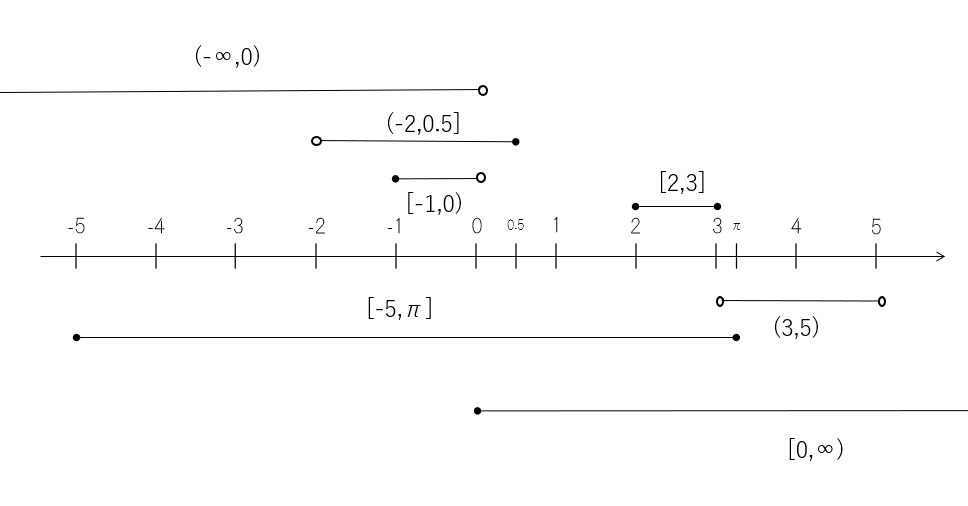
\includegraphics[keepaspectratio,scale=0.6]{img/QuuNote/kihonmondaikaitouzu_1.png}
                        \caption{数直線}
                    \end{figure}

                    $1.\quad [2,3]$\hspace{3mm}
                    $2.\quad (3,5)$\hspace{3mm}
                    $3.\quad [-5,\pi]$\hspace{3mm}
                    $4.\quad (-2,0.5]$\hspace{3mm}
                    $5.\quad [-1,0)$\hspace{3mm}
                    $6.\quad (-\infty,0)$\hspace{3mm}
                    $7.\quad [0,\infty)$\hspace{3mm}
            \clearpage
            \basicanswer
                \paragraph{問1}次の関数が偶関数か奇関数かを判別せよ。

                \noindent
                (1)偶\hspace{3mm}
                (2)奇\hspace{3mm}
                (3)奇\hspace{3mm}
                (4)偶\hspace{3mm}
                (5)奇\hspace{3mm}
                (6)どちらでもない\hspace{3mm}
                (7)偶\hspace{3mm}
                (8)奇

                \paragraph{問2}以下の等式を証明せよ。

                \noindent
                $(1)$加法定理で$\alpha=\beta=x$と置く。$\sin(2x)=\sin x\cos x+\cos x\sin x=2\sin x\cos x$\hspace{1mm}$\cos 2x$も同様。\\
                $(2)$倍角の公式より、$\cos 2x=\cos^2 x-\sin^2 x=1-2\sin^2 x$変形して$x$に$\frac{x}{2}$を代入すれば半角の公式が得られる。$\cos^2 \frac{x}{2}$も同様。\\
                $\displaystyle(3)\sinh(x+y)=\frac{e^{x+y}-e^{-(x+y)}}{2}=\frac{e^{x+y}-e^{x-y}+e^{x-y}-e^{-x-y}}{2}=\frac{e^{x}(e^{y}-e^{-y})+e^{-y}(e^x-e^{-x})}{2}=e^x\sinh y+e^{-y}\sinh x=2\cosh x\sinh y -e^{-x}\sinh y+2\cosh y\sinh x -e^{y}\sinh x$\\
                ここで$\displaystyle e^{-x}\sinh y+e^{y}\sinh x=\frac{e^{y-x}-e^{-y-x}}{2}+\frac{e^{x+y}-e^{y-x}}{2}=\sinh(x+y)$である。\\
                よって、$\displaystyle \sinh (x+y)=2\cosh x\sinh x+2\cosh y\sinh x-\sinh (x+y)\to \sinh(x+y)=\cosh x\sinh x+\cosh y\sinh x$となる。$\cosh (x+y)$についても同様。
                
                \paragraph{問3}以下の値を求めよ。

                \noindent
                $(1)0$\hspace{3mm}
                $(2)\frac{\pi}{6}$\hspace{3mm}
                $(3)0$\hspace{3mm}
                $(4)3$\hspace{3mm}
                $(5)0$\hspace{3mm}
                $(6)1$\hspace{3mm}
                $(7)\frac{\pi}{2}-\cos\log 3\sin\log 2$
                
                \paragraph{問4}$I=271\times 314$と置けば、$\log_{10} I=\log_{10}2.71+\log_{10}3.14+4$である。よって、$\log_{10}I=4.9315$より$I=10^{4.9315}\simeq 85408$
                
                \paragraph{問5}$t=\tan\frac{x}{2}$とするとき、$\sin x,\cos x,\tan x$をそれぞれ$t$を用いた式で表せ。
                \begin{align*}
                    \sin x &=2\sin \frac{x}{2}\cos \frac{x}{2}=\frac{2\tan\frac{x}{2}}{\frac{1}{\cos^2\frac{x}{2}}}=\frac{2t}{1+t^2}\\
                    \cos x &=\cos^2 \frac{x}{2} -\sin^2 \frac{x}{2}=\frac{1-\tan^2\frac{x}{2}}{\frac{1}{\cos ^2\frac{x}{2}}}=\frac{1-t^2}{1+t^2}\\
                    \tan x &=\frac{\sin x}{\cos x}=\frac{\displaystyle\frac{2t}{1+t^2}}{\displaystyle\frac{1-t^2}{1+t^2}}=\frac{2t}{1-t^2}
                \end{align*}
            \clearpage
            \basicanswer 
            
                \paragraph{問1}以下の数列の一般項を示し、それらが収束するかどうか答えよ。\\
                $(1)\frac{n+1}{n}=1+\frac{1}{n}$収束する\hspace{3mm}
                $(2)\frac{1}{3^n}$収束する\hspace{3mm}
                $(3)(-1)^{n+1}$発散する\hspace{3mm}
                $(4)a+(n-1)d$発散する

                \paragraph{問2}仮定より$\displaystyle |a-a_n|<\frac{\varepsilon}{2}\quad(n>N_1),|b-b_n|<\frac{\varepsilon}{2}\quad(n>N_2)$となる$N_1,N_2$が存在する。ここで、$N_1,N_2$のうち大きい方をとり
                \footnote{ここで大きい方を取ることで、必ず仮定の条件を満たす。例えば$N_1>N_2$であるとき$N=N_1$と取れば、どちらの数列に対しても$\ldots<\frac{\varepsilon}{2}$となるが、$N=N_2$と取ってしまうと$N_1>n>N_2$であるような$n$に対して$|a-a_n|<\frac{\varepsilon}{2}$が保証できないのである。}
                、それを$N=\max(N_1,N_2)$と置けば$n>N$のとき
                \begin{equation*}
                    |(a+b)-(a_n+b_n)|=|(a-a_n)+(b-b_n)|\leq |a-a_n|+|b-b_n|<\frac{\varepsilon}{2}+\frac{\varepsilon}{2}=\varepsilon
                \end{equation*}
                となるような$N$が存在する。よって、証明完了。

                \paragraph{問3}以下計算せよ。\\

                \noindent
                $(1)2$\hspace{3mm}
                $(2)4\pi^2$\hspace{3mm}
                $(3)0$\hspace{3mm}
                $(4)2$\hspace{3mm}
                $(5)0$\hspace{3mm}
                $(6)-1$\hspace{3mm}
                $(7)\frac{1}{2}$\hspace{3mm}
                $(8)1$
                
                \paragraph{問4}次の関数が()内の点において連続であるかどうか調べよ。\\
                $(1)$連続\hspace{1mm}
                $(2)$連続\hspace{1mm}
                $(3)$連続\hspace{1mm}
                $(4)$不連続\hspace{1mm}
                $(5)$連続\\
                $(6)\displaystyle \lim_{x\to 0}f(x)=\lim_{x\to 0}x\sin\frac{1}{x}$に注意する。また、$-1\leq\sin\frac{1}{x}\leq 1$であるため、$-x\leq f(x) \leq x$
                ここで$x\to 0$の極限を取れば$x,-x\to 0$なのではさみうちの原理より$f(x)\to 0.$これは$f(0)=1$と一致しないので、\underbar{不連続}

                \paragraph{問5}方程式$\sin x=x$が区間$[0,\frac{\pi}{2}]$に実数解をもつかどうか調べよ。

                $x=0$で等号が成り立つので実数解は存在する。\\
                (補足)$\cos x=x$の場合でも実数解をもつか考えてみることにする。
                $f(x)=\cos x-x$と置くと、$f(x)$は$[0,\frac{\pi}{2}]$で連続であり
                \begin{equation*}
                    f(0)=1>0,\quad f\left(\frac{\pi}{2}\right)=-\frac{\pi}{2}<0
                \end{equation*}
                したがって中間値の定理より区間$[0,\frac{\pi}{2}]$に$\cos x=x$は実数解をもつ。
        \clearpage
        \subsection{微分法 基本問題解答}
            \basicanswer
                \paragraph{問1}次の関数の(\hspace{2mm})内の区間での平均変化率を求めよ。\\
                $(1)4$\hspace{3mm}
                $(2)2$\hspace{3mm}
                $(3)\frac{\sqrt{3}-1}{\pi/3}$

                \paragraph{問2}次の関数を微分せよ。\\
                \noindent
                $(1)y'=1$\hspace{5mm}
                $(2)y'=0$\hspace{5mm}
                $(3)y'=3x^2$\hspace{5mm}
                $(4)y'=a$\hspace{5mm}
                $(5)y'=2a(x+p)q$

                
                \paragraph{問3}$y=\sqrt{x}\hspace{1mm}(x\geq 0)$が微分可能であるか調べよ。

                $x=0$について微分可能性を調べると
                \begin{equation*}
                    \lim_{h\to +0}\frac{\sqrt{0+h}-\sqrt{0}}{h}=\lim_{h\to+0}\frac{\sqrt{h}}{h}=\lim_{h\to+0}\frac{1}{\sqrt{h}}
                \end{equation*}
                この極限は存在しないので、$\sqrt{x}$は($x=0$で)微分可能ではない。

                \paragraph{問4}
                \begin{equation*}
                    \frac{d}{dx}(af(x))=\lim_{h\to 0}\frac{af(x+h)-af(x)}{h}=a\lim_{h\to 0}\frac{f(x+h)-f(x)}{h}=a\frac{d}{dx}f(x)
                \end{equation*}
            \clearpage
            \basicanswer
                \paragraph{問1}以下の関数の導関数を求めよ。\\
                $(1)y'=2x$\hspace{2mm}
                $(2)y'=-\sin x+\cos x$\hspace{2mm}
                $(3)y'=\frac{1}{x}$\hspace{2mm}
                $(4)y'=\frac{-1}{\sqrt{1-x^2}}$\hspace{2mm}
                $(5)y'=\frac{e^{\tan x}}{\cos^2 x}$\\
                $(6)y'=2e^{x^2}(x\cos2x-\sin 2x)$\hspace{3mm}
                $(7)y'=\frac{1}{\sqrt{x^2+1}}$\hspace{3mm}
                $(8)y'=\frac{1}{4\sqrt[4]{x^3}}$

                \paragraph{問2}以下を示せ。\\
                (1)$\displaystyle\frac{\frac{f(x+h)}{g(x+h)}-\frac{f}{g}}{h}=\frac{f(x+h)g-fg(x+h)}{hgg(x+h)}=\frac{g\cdot(f(x+h)-f)-f\cdot(g(x+h)-g)}{hgg(x+h)}$として$h\to0$の極限を取る。もしくは積の微分公式を利用してもよい。\\
                (2)$\displaystyle\frac{e^{a(x+h)}-e^{ax}}{h}=ae^{ax}\frac{e^{ah}-1}{ah}$であり、$h\to0$のとき$ah\to 0$であるため、$(e^{ax})'=ae^{ax}$\\
                (3)$\sin^2 x+\cos ^2 x=1$の両辺を$x$微分すると$2\sin x\cos x+2\cos x(\cos x)'=0$仮定より$\cos x\neq 0$なので、両辺を$2\cos x$で割って移項すると$(\cos x)'=-\sin x$

                \paragraph{問3}以下の関数の導関数を工夫して求めよ。\\
                $\displaystyle(1)y'=\frac{2(x-1)}{3(x+1)\sqrt[3]{(x+1)^2(x^2+1)^2}}$\hspace{3mm}
                $(2)y'=x^x(\log x+1)$\\
                $(3)x=\tan \theta$と置くと、$\displaystyle y=\sin^{-1}\frac{\tan \theta}{\sqrt{1+\tan^2\theta}}=\theta$なので、\\
                $\displaystyle \frac{dy}{dx}=\frac{dy}{d\theta}\frac{d\theta}{dx}=1\cdot\frac{1}{\frac{dx}{d\theta}}=\cos^2 \theta=\frac{1}{1+\tan^2\theta}=\frac{1}{1+x^2}$よって$\displaystyle y'=\frac{1}{1+x^2}$

                \paragraph{問4}双曲線関数について、$\sinh x,\cosh x$の導関数を導出せよ。

                $\sinh x,\cosh x$の定義から求めよ。$(\sinh x)'=\cosh x,(\cosh x)'=\sinh x$

                \paragraph{問5}
                \begin{enumerate}\setcounter{enumi}{0}\renewcommand{\labelenumi}{(\arabic{enumi})}
                    \item 右辺に加法定理を適用して示せ。
                    \item $\displaystyle\cos\alpha\cos\beta=\frac{1}{2}\{\cos(\alpha+\beta)+\cos(\alpha-\beta)\}$
                    \item $\displaystyle\sin\alpha\sin\beta=-\frac{1}{2}\{\cos(\alpha+\beta)-\cos(\alpha-\beta)\}$
                \end{enumerate}
            \clearpage
            \basicanswer 以下の問いに答えよ。

                \paragraph{問1}次の関数のグラフをかけ。\\
                省略

                \paragraph{問2}次の関数の(\hspace{1mm})内での最大・最小を求めよ。\\
                増減表を書いて求めよ。\\
                $(1)$最大値:$\left(\frac{3}{5}\right)^{\frac{5}{2}}-\left(\frac{3}{5}\right)^{\frac{3}{2}}$ 最小値:$-\left(\frac{3}{5}\right)^{\frac{5}{2}}+\left(\frac{3}{5}\right)^{\frac{3}{2}}$\hspace{3mm}
                $(2)$最大値:$e^2\hspace{1mm}(x=2)$ 最小値:$-1\hspace{1mm}(x=0)$

                \paragraph{問3}$e^x \geq x+1 \quad (x\geq0)$を示せ。\\
                $f(x)=e^x-x+1$と置く。この時、$f'(x)=e^x-1=0\leftrightarrow x=0$であり、$x>0$で$f'(x)>0$であるので、$f(x)$は
                $x>0$で単調増加する。よって、$f(x)$の最小値は$x=0$のときであり、その値は$f(0)=e^0-0+1=0$である。
                すなわち$f(x)\geq 0\leftrightarrow e^x\geq x+1$

                \paragraph{問4}図\ref{fig:直流回路}の直流回路について、最初に流れる電流$I$は以下の式で表される。
                \begin{equation*}
                    I=\frac{E}{R_0+R}\quad(\text{オームの法則})
                \end{equation*}
                また、可変抵抗器$R$で消費される電力$P$は$P=I^2R$である。この時、可変抵抗器で消費される最大の電力$P_{max}$
                の値を求めよ。また、この時の可変抵抗器の値を求めよ。

                \begin{equation*}
                    \frac{dP}{dR}=\frac{d}{dR}\left(\frac{E^2R}{(R_0+R)^2}\right)=\frac{E^2(R_0+R)^2-E^2R\cdot2(R_0+R)}{(R_0+R)^4}=\frac{E^2(R_0-R)}{(R_0+R)^3}=0
                \end{equation*}
                $R_0>R>0$のとき$P'>0$であり$R>R_0$のとき$P'<0$なので、$P$は$R=R_0$で最大値を取る。またその値は
                \begin{equation*}
                    P_{max}=\frac{E^2R_0}{(R_0+R_0)^2}=\frac{E^2}{4R_0}
                \end{equation*}
                一般に、直流回路網は図\ref{fig:直流回路}の回路の回路に直せるので、その際にこの公式が使われる。
            \clearpage
            \basicanswer
                \paragraph{問1}次の関数の三次導関数を求めよ。\\
                $(1)y'''=48$\hspace{3mm}
                $(2)\displaystyle y'''=\frac{-6}{(1+x)^4}$\hspace{3mm}
                $(3)y'''=-8\cos(2x)$\hspace{3mm}
                $(4)y'''=e^x(x+3)$\\
                $\displaystyle(5)y'''=\frac{12\sin(2x)}{(1+x)^2}-\frac{6\sin(2x)}{(1+x)^4}-\frac{8\cos(2x)}{1+x}+\frac{12\cos(2x)}{(1+x)^3}$

                \paragraph{問2}次の関数の$n$次導関数を求めよ。\\
                $(1)y^{(n)}=(-1)^ne^{-x}$\hspace{3mm}
                $(2)y=\cos\left(x+\frac{n\pi}{2}\right)$\hspace{3mm}
                $(3)y=n!$\hspace{3mm}
                $(4)y=\frac{(-1)^{n-1}(n-1)!}{(x+1)^{n}}$

                \paragraph{問3}次の極限をロピタルの定理を用いて求めよ。\\
                $(1)\frac{1}{2}$\hspace{2mm}
                $(2)1$\hspace{2mm}
                $(3)0$\hspace{2mm}
                $\displaystyle(4)\lim_{x\to+0}x^x=e^{x\log x}=\lim_{x\to+0}e^{\frac{\log x}{\frac{1}{x}}}$と変形。$\displaystyle\lim_{x\to+0}\frac{\log x}{\frac{1}{x}}=\lim_{x\to+0}x=0$より、答えは$e^{0}=1$
                $\displaystyle(5)\lim_{x\to\infty}\log(1+e^x)^{\frac{1}{x}}=\lim_{x\to\infty}\frac{\log(1+e^x)}{x}=\lim_{x\to\infty}\frac{e^x}{1+e^x}=\lim_{x\to\infty}\frac{e^x}{e^x}=1$

                \paragraph{問4}定数項がない$x$の多項式について$n\to0,\infty$で減少の速さが$x$で抑えられるとき$P(x)$と書く。\footnote{これはあいまいな表現であり、もっと厳密にランダウの記号として数学で定義されている。ここではfeelingで書いた。ちなみにこのランダウは理論物理学で有名なランダウではなく、数学者のランダウである。}\\
                \vspace{1mm}$(1)$$\sin x=x-\frac{1}{3!}x^3+P(x^5)$と書けるので\\
                $\displaystyle\lim_{x\to 0}\frac{x-\sin x}{x^3}=\lim_{x\to 0}\frac{x-\left(x-\frac{1}{3!}x^3+P(x^5)\right)}{x^3}=\lim_{x\to 0}\frac{\frac{1}{3!}x^3-P(x^5)}{x^3}=\lim_{x\to 0}\left\{\frac{1}{3!}-P(x^2)\right\}=\frac{1}{3!}$\\
                \vspace{3mm}\noindent
                $(2)\displaystyle\sqrt{x^2-3x+1}=x\sqrt{1-\left(\frac{3}{x}-\frac{1}{x^2}\right)}$と変形する。このとき$\sqrt{1-x}=1-\frac{1}{2}x-\frac{1}{2!}\cdot\frac{3}{4}x^2\cdots$より\\
                $\displaystyle x\sqrt{1-\left(\frac{3}{x}-\frac{1}{x^2}\right)}=x\left\{1-\frac{1}{2}\left(\frac{3}{x}-\frac{1}{x^2}\right)-\frac{1}{2!}\cdot\frac{3}{4}\left(\frac{3}{x}-\frac{1}{x^2}\right)^2+\cdots\right\}=x\left\{1-\frac{1}{2}\times\frac{3}{x}-P\left(\frac{1}{x^2}\right)\right\}$\\
                $\displaystyle=x-\frac{3}{2}-P\left(\frac{1}{x}\right)$したがって、元の極限は
                $\displaystyle\lim_{x\to \infty}\left\{x-\frac{3}{2}-P\left(\frac{1}{x}\right)-x\right\}=-\frac{3}{2}$

                \paragraph{問5}省略
                
                \paragraph{問6}
                $g(x)$は$[a,b]$で連続で、$(a,b)$で$n+1$階微分可能である。この時、$g(b)=0$がすぐわかる。また、少し計算すれば$g(a)=0$
                もわかる。すなわち$g(a)=g(b)$であるため、ロルの定理より
                \begin{equation*}
                    g'(c)=0\quad(a<c<b)
                \end{equation*}
                である。よって、
                \begin{align*}
                    g'(c)&=f'(c)-f'(c)+f''(c)(b-c)-f''(c)(b-c)+\frac{1}{2!}f'''(c)(b-c)^2+\cdots-\frac{1}{(n-1)!}f^{(n)}(c)(b-c)^{n-1}\\
                    &+\frac{1}{n!}f^{(n+1)}(c)(b-c)^{n}-K(n+1)(b-c)^{n}=0
                \end{align*}
                式を整理して
                \begin{equation*}
                    K=\frac{1}{(n+1)!}f^{(n+1)}(c)
                \end{equation*}
                これを$K$の定義に代入して整理すれば、式\eqref{eq:テイラーの定理}である。$\square$
            \clearpage

        \clearpage
        \subsection{積分 基本問題解答}
            \basicanswer
                \paragraph{問1}次の不定積分を求めよ。\\
                    $(1)\displaystyle \frac{1}{4}x^4$\hspace{3mm}
                    $(2)\displaystyle \cos x$\hspace{3mm}
                    $(3)\displaystyle \frac{1}{2}e^{x}-\frac{1}{x}$\hspace{3mm}
                    $(4)\displaystyle \frac{\log x}{e}$\hspace{3mm}
                    $(5)\displaystyle \tan^2 x + 1=\frac{1}{\cos^2 x}$より$\tan x$\hspace{3mm}
                    $(6)\displaystyle \sin x\cos x=\frac{1}{2}\sin 2x$より$\displaystyle -\frac{1}{4}\cos 2x$

                \paragraph{問2}次の不定積分を(\hspace{1mm})内の置換によって求めよ。\\
                    $(1)\displaystyle \frac{1}{2}\sin(x^2)$\hspace{3mm}
                    $(2)\displaystyle \frac{1}{9}(x^3-1)^3$\hspace{3mm}
                    $(3)\displaystyle \tan^{-1}x$ \hspace{3mm}
                    $(4)\displaystyle \sin^{-1} x$\hspace{3mm}
                    $(5)\displaystyle \frac{1}{4}\sin^4 x$
                
                \paragraph{問3}次の不定積分を部分積分法で求めよ。\footnote{$(3)$はほかにも面白い解きかたがある。例えば、オイラーの公式を使えば積分は$\Re\int e^{(i+1)x}dx$と表せるので、これを解けばよい。}\\
                    $(1)\displaystyle x\sin x+\cos x$\hspace{3mm}
                    $(2)\displaystyle (x-1)e^x$\\
                    $(3)\displaystyle I=e^x\cos x+\int e^x\sin xdx=e^x\cos x+e^x\sin x - \int e^x\cos xdx=e^x(\sin x+\cos x)-I$\\$\therefore I=\frac{e^x}{2}(\sin x+\cos x)$\\
                    $(4)\displaystyle \int=x\log(x^2+1)-2\int \frac{x^2}{x^2+1}dx=x\log(x^2+1)-2\int\left(1-\frac{1}{x^2+1}\right)dx=x\log(x^2+1)-2x+2\tan^{-1}x$\\
                    $(5)\displaystyle I=\int \sqrt{a^2-x^2}dx=x\sqrt{a^2-x^2}+\int \frac{x^2}{\sqrt{a^2-x^2}}dx=x\sqrt{a^2-x^2}-\int\left[\sqrt{a^2-x^2}-\frac{a^2}{\sqrt{a^2-x^2}}\right]dx=x\sqrt{a^2-x^2}+a^2\sin^{-1}\left(\frac{x}{a}\right)-I$
                    したがって、$\displaystyle I=\frac{1}{2}\left[x\sqrt{a^2-x^2}+a^2\sin^{-1}\left(\frac{x}{a}\right)\right]$

                \paragraph{問4}次の不定積分を部分分数分解を用いて求めよ。\\
                    $(1)\displaystyle \log\left|\frac{2-x}{1-x}\right|$\hspace{3mm}
                    $(2)\displaystyle \frac{1}{(x^2+1)(x-2)}=\frac{Ax+B}{x^2+1}+\frac{C}{x-2}$と置けば、$A=\frac{-1}{5},B=\frac{-2}{5},C=\frac{1}{5}$となるので、答えは$\displaystyle \frac{1}{10}\left(-\log(x^2+1)+2\log|x-2|-4\tan^{-1}x\right)$\hspace{3mm}
                    $(3)\displaystyle \frac{1}{2a}\log\left|\frac{x-a}{x+a}\right|$

                \paragraph{問5}以下証明せよ。
                    \begin{enumerate}\setcounter{enumi}{0}\renewcommand{\labelenumi}{(\arabic{enumi})}
                        \item $\sinh x$の定義から導け。
                        \item $t=\tan\frac{x}{2}$と置くと、
                        \begin{equation*}
                            \sin x = \frac{2t}{1+t^2},\quad \cos x = \frac{1-t^2}{1+t^2}
                        \end{equation*}
                        と表せる。また、$t = \tan\frac{x}{2} \rightarrow x = 2\tan^{-1}t $より
                        \begin{equation*}
                            dx = \frac{2}{1+t^2}dt
                        \end{equation*}
                        したがって、元の積分は
                        \begin{equation*}
                            \int f\left(\frac{2t}{1+t^2},\frac{1-t^2}{1+t^2}\right)\frac{2dt}{1+t^2}
                        \end{equation*}
                        となるので、被積分関数は$t$の有理関数に帰着する。よって、必ず積分できる。$\square$
                    \end{enumerate}
                \clearpage
                \basicanswer
                    \paragraph{問1}
                    性質\eqref{eq:関数と積分値の大小関係}は、式を移項して$\int (f-g)dx \geq 0$を示せ。性質\eqref{eq:int[a,a]=0}は、\eqref{eq:int[a,b]=-[b,a]}で$b=a$とし、移項せよ。

                    \paragraph{問2}区間$[0,1]$をちょうど$n$等分すると$x_k=\frac{k}{n}$であり、$\Delta x_k = \frac{1}{n}$となる。したがって、$\displaystyle \int_0^1 xdx = \lim \sum \left(\frac{k}{n}\right) \frac{1}{n}=\lim \frac{1}{n^2} \sum k=\lim_{n\to 0}\frac{n(n+1)}{2n^2}=\frac{1}{2}$

                    \paragraph{問3}以下の定積分の値を求めよ。ただし$0\leq \epsilon < 1$である。\\
                    $(1)\displaystyle 2$\hspace{3mm}
                    $(2)\displaystyle \frac{\pi}{6}$\hspace{3mm}
                    $(3)\displaystyle 2(e^2-1)$\hspace{3mm}
                    $(4)\displaystyle \frac{726}{5}$\hspace{3mm}
                    $(5)t=\tan\frac{x}{2}$と置け。$\displaystyle \frac{\pi}{\sqrt{1-\epsilon^2}}$\\
                    それにしてもあのsinの曲線下の面積(1)がこんなに簡単に求まるなんて、ただただ驚くばかりである。

                    \paragraph{問4}次の広義積分を求めよ。\\
                    $(1)\displaystyle -\frac{1}{3}$\hspace{3mm}
                    $(2)\displaystyle \int_0^1 \log xdx$\hspace{3mm}
                    $(3)\displaystyle \lim_{\varepsilon\to +0}\varepsilon\log \varepsilon = 0$を用いよ。$-1$\\
                    $(4)x=a\sin^2 \theta\quad(0\leq\theta\leq \frac{\pi}{2})$と置換すると$dx = 2a\sin\theta\cos\theta d\theta$より、\\$\displaystyle \int_0^{\frac{\pi}{2}} \frac{2a\sin\theta\cos\theta}{\sqrt{a^2\sin^2\theta-a^2\sin^4\theta}}d\theta=2\int_{0}^{\frac{\pi}{2}}d\theta =\pi$\\
                    $(5)$普通に部分分数分解してもよいが、ここでは違った解き方を示そう。積分変数は何でもよいので、$x\to \frac{1}{x}$の置換を行うと、
                    \begin{equation*}
                        \int_{0}^{\infty}\frac{dx}{x^3+1}=\int_{\infty}^{0}\frac{-\frac{1}{x^2}}{\left(\frac{1}{x}\right)^3+1}dx=\int_{0}^{\infty}\frac{x}{x^3+1}dx
                    \end{equation*}
                    よって、最初の積分と足し合わせると
                    \begin{equation*}
                        \frac{1}{2}\int_{0}^{\infty}\frac{x+1}{x^3+1}dx=\frac{1}{2}\int_{0}^{\infty}\frac{dx}{x^2-x+1}=\frac{1}{2}\int_{0}^{\infty}\frac{dx}{\left(x-\frac{1}{2}\right)^2+\frac{3}{4}}=\left[\frac{1}{\sqrt{3}}\tan^{-1}\frac{x-\frac{1}{2}}{\frac{\sqrt{3}}{2}}\right]_0^\infty=\frac{\pi}{2\sqrt{3}}+\frac{\pi}{6\sqrt{3}}=\frac{2\pi}{3\sqrt{3}}
                    \end{equation*}

                    \paragraph{問5}三角関数の公式を用いて$\cos$の和の形に直し、それぞれ場合分けせよ。

                    \paragraph{問6}次の積分(広義積分)が収束するための$k$の範囲を求めよ。
                    \begin{equation*}
                        \int_1^\infty \frac{dx}{x^{k}}=\lim_{b\to\infty}\left[\frac{1}{1-k}\frac{1}{x^{k-1}}\right]_1^b=\lim \frac{1}{1-k}\left(\frac{1}{b^{k-1}}-1\right)
                    \end{equation*}
                    よって、収束するためには$k-1>0$であればよいので、$k>0$.

                    \paragraph{問7}関数$f(x)$が偶関数であることを$f=f_e$、奇関数であることを$f=f_o$と表記することにする。この時以下を示せ。
                    \begin{equation*}
                        \int_{-a}^a f(x)dx = \int_{0}^{a}+\int_{-a}^{0}
                    \end{equation*}
                    であるため、右辺二項目の積分に$x\to -x$の置換を行うと、
                    \begin{equation*}
                        \int_{-a}^{a}f(x)dx = \int_0^a f(x)dx - \int_{a}^{0}f(-x)dx=\int_{0}^{a}\left\{f(x)+f(-x)\right\} dx
                    \end{equation*}
                    $f=f_e$なら$f(-x)=f(x)$、$f=f_o$なら$f(-x)=-f(x)$であるため、公式\eqref{eq:定積分と偶関数・奇関数}を得る。

                    \paragraph{問8}次の問いに答えよ。
                    \begin{enumerate}\setcounter{enumi}{0}\renewcommand{\labelenumi}{(\arabic{enumi})}
                        \item $\displaystyle \cos x = t$と置け。$\displaystyle \frac{\pi}{2}$
                        \item 置換$x\to\pi -x$を行うと、$\sin(\pi-\theta)=\sin\theta$より、$\displaystyle I=\int_{0}^{\pi}xf(\sin x)dx=\int_{0}^{\pi}(\pi-x)f(\sin(\pi-x))dx = \pi\int_{0}^{\pi}f(\sin x)dx - I.$したがって$\displaystyle I=\frac{\pi}{2}\int_{0}^{\pi}f(\sin x)dx$
                        \item $(1),(2)$の結果を用いる。$\displaystyle\frac{\pi^2}{4}$
                    \end{enumerate}
                \clearpage
                \basicanswer
                    \paragraph{問1}$\displaystyle\frac{x^2}{a^2}+\frac{y^2}{b^2}=1$を変形して、楕円の上半分$(t>0)$の式を求めると$\displaystyle y = \frac{b}{a}\sqrt{a^2-x^2}$となる。あとは$[-a,a]$で積分すれば
                    \begin{equation*}
                        \frac{b}{a}\int_{-a}^{a}\sqrt{a^2-x^2}dx
                    \end{equation*}
                    ところで積分は半径$a$の半円の面積に等しい。したがって、$ab\pi$

                    \paragraph{問2}求める面積は放物線で囲まれた`アメーバ'のような形をしている。二つの放物線が交わるのは
                    $4px = x^2$のとき。すなわち、$x=0,4p$のときであるため、
                    \begin{equation*}
                        \int_{0}^{4p}\left(2\sqrt{px}-\frac{1}{4p}x^2\right)dx = \left[\frac{4}{3}\sqrt{p}\cdot x\sqrt{x}-\frac{x^3}{12p}\right]_0^{4p}=\frac{16}{3}p^2
                    \end{equation*}

                    \paragraph{問3}半径$r$の球は、$y=\sqrt{r^2-x^2}$をx軸周りに回転させた回転体に等しい。よって、
                    \begin{equation*}
                        \pi\int_{-r}^{r}\left\{r^2-x^2\right\}dx = 2\pi\left[r^2x-\frac{x^3}{3}\right]_0^r = \frac{4\pi r^3}{3}
                    \end{equation*}

                    \paragraph{問4}$y'=\sinh x$より、
                    \begin{equation*}
                        \int_{-1}^{1}\sqrt{1+\sinh^2 x}dx =\int_{-1}^{1}\cosh xdx = \sinh(1)-\sinh(-1)=2\sinh 1 \left(=e-\frac{1}{e}\right)
                    \end{equation*}

                    \paragraph{問5}求める円錐は、直線$y=\frac{r}{h}x$を区間$[0,h]$においてx軸周りに回転させた回転体の体積に等しい。
                    \begin{equation*}
                        \pi\int_{0}^{h}\frac{r^2}{h^2}x^2dx = \frac{\pi r^2}{h^2}\cdot \frac{h^3}{3}=\frac{1}{3}\pi r^2h
                    \end{equation*}

                    \paragraph{問6}以下(Excelで計算した結果)を参照。なお真値は$\pi\approx 3.141592653589793238462643$\footnote{参考:\url{https://www.tstcl.jp/ja/randd/pi.php}}
                    \begin{figure}[h]
                        \centering
                        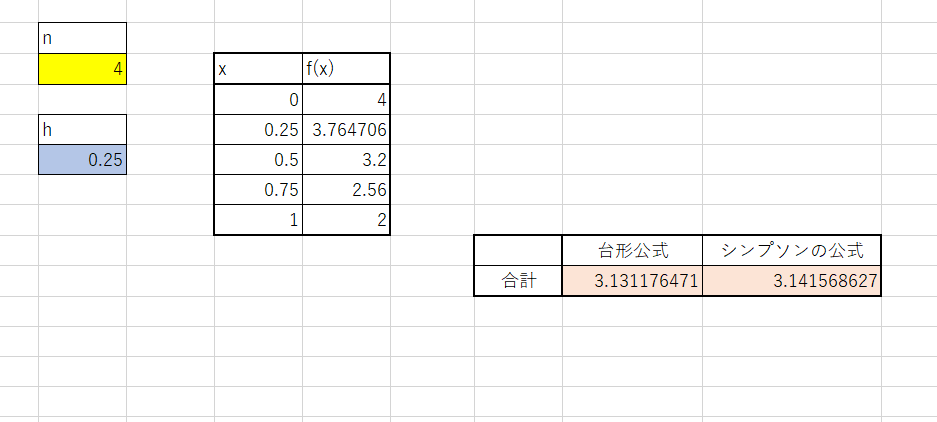
\includegraphics[scale=0.5]{img/QuuNote/kihonmondai_ten.png}
                    \end{figure}
                

                        
        \clearpage
        \subsection{無限級数 基本問題解答}
            \basicanswer 

                \paragraph{問1}次の無限級数が収束するか発散するかを調べ、収束するならその和を答えよ。\\
                $(1)\lim n \neq 0$より発散。\hspace{3mm}
                $(2)\lim (-1)^n\neq 0$より発散。\hspace{3mm}
                $(3)\displaystyle \lim \frac{n}{n+1}\neq 0$より発散。\\
                $(4)\displaystyle\frac{1}{n(n+1)}=\frac{1}{n}-\frac{1}{n+1}$より、$S_n = 1-\frac{1}{n+1}$である。したがって収束して和は$1$\\
                $(5)\displaystyle \frac{n}{(n+1)!}=\frac{n\cdot n!}{(n+1)!\cdot n!}=\frac{1}{n!}-\frac{1}{(n+1)!}$より、$S_n=1-\frac{1}{(n+1)!}$である。したがって収束して和は$1$

                \paragraph{問2}以下の数列が収束することを示せ。\\
                $\displaystyle (1)a_{n+1}-a_n = \frac{n+1}{2n+3}-\frac{n}{2n+1}=\frac{2n^2+3n+1-2n^2-3n}{(2n+3)(2n+1)}=\frac{1}{(2n+3)(2n+1)}>0$したがって、$a_n$は単調増加である。
                さらに、$\displaystyle a_n = \frac{n}{2n+1}=\frac{1}{2}\left(1-\frac{1}{2n+1}\right)$より、$a_n < \frac{1}{2}$である。単調増加だから下界ももちろん存在する。したがって、$a_n$は有界である。
                よって、収束する。$(2),(3)$も同様。

                \paragraph{問3}仮定より級数の$n$部分和を$S_n$と表せば、$\lim S_n$は収束する。ここで、$S_n - S_{n-1} = a_n$であるため、
                $\lim a_n = \lim \{S_n-S_{n-1}\}=S-S=0$である。$\square$

                \paragraph{問4}等比数列の和の公式より、$S_n = \frac{a(1-r^n)}{1-r}$である。したがって、等比級数が収束するかどうかは$r^n$が収束するかどうかと(ほぼ)同じである。この時、$|r|\leq 1$であれば、$r^n$は収束する。
                しかし、$r=1$のとき分母が$0$になるので、答えは$|r|<1$

                \paragraph{問5}移動する初めの場所から目的地までの距離を$l$とする。$n$回目の移動で進む距離は$\frac{l}{2^n}$である。よって、$n$回の移動で最初の地点から
                進んだ合計の距離は$\displaystyle \sum_1^n \frac{l}{2^n}$と表せる。よって、$n\to\infty$の極限を取ると級数は収束してその値は$l$となる。つまり、ゼノンの``論法''を繰り返しても、
                結局最初の目標地点に到達することができる。
            \clearpage
            \basicanswer 
                \paragraph{問1}比較法を用いて、次の級数の収束、発散を調べよ。\\
                $\displaystyle(1)\frac{1}{\log n}>\frac{1}{n}$より、発散\hspace{15mm}
                $\displaystyle(2)\frac{\log n}{n^3+1}<\frac{n}{n^3}=\frac{1}{n^2}$より収束\hspace{15mm}
                $\displaystyle(3)\frac{n^2+1}{n^3+1}\geq  \frac{1}{n}$より、発散

                \paragraph{問2}コーシーの判定法かダランベールの判定法を用いて、次の級数の収束、発散を調べよ。\\
                $\displaystyle(1)$コーシーの判定法を用いる。$L=\lim \sqrt[n]{n^{-n}}=0$よって収束\\
                $\displaystyle(2)$ダランベールの判定法を用いる。$L=\lim \frac{(n+1)^5e^{-(n+1)^2}}{n^5e^{-n^2}}=0$よって収束\\
                $\displaystyle(3)$コーシーの判定法を用いる。$L=\lim \sqrt[n]{\left(\frac{n}{2n+1}\right)^n}=\frac{1}{2}<1$よって収束

                \paragraph{問3}積分判定法より、次の級数の収束、発散を調べよ。\\
                $\displaystyle(1)\int_1^\infty \frac{x}{x^2+2}dx = \left[\frac{1}{2}\log(x^2+2)\right]_1^\infty$よって発散\\
                $\displaystyle(2)\int_1^\infty xe^{-x^2}dx = \left[\frac{1}{2}e^{-x^2}\right]_1^\infty=\frac{1}{2e}$よって収束\\
                $\displaystyle(3)\int_2^\infty \frac{dx}{x\log x}=\left[\log\log x\right]_2^\infty$よって発散

                \paragraph{問4}$\lim n^p a_n$を計算することで、次の級数の収束、発散を調べよ。\\
                $\displaystyle(1)\lim n^2 \cdot\frac{n}{3n^3-1}=\frac{1}{3}$よって収束\hspace{5mm}
                $\displaystyle(2)\lim \sqrt{n}\cdot\frac{\log n}{\sqrt{n+2}}=\infty$よって発散\hspace{5mm}
                $\displaystyle(3)\lim n^3\cdot \sin^3\left(\frac{1}{n}\right)=1$よって収束

                \paragraph{問5}次の級数の収束、絶対収束を調べよ。\\
                $\displaystyle(1)$絶対収束する。\hspace{5mm}
                $\displaystyle(2)$絶対収束する。\hspace{5mm}
                $\displaystyle(3)$絶対収束しない。しかし、$\lim \frac{1}{n}=0$であり、$0< \frac{1}{n+1}< \frac{1}{n}$であるから、収束する。したがって条件収束。
                
                \paragraph{問6}次の収束・発散を調べよ。\\
                $\displaystyle (1)$ダランベールの判定法を用いる。$\displaystyle L=\lim\frac{(a+1)(2a+1)\cdots((n+1)a+1)}{(b+1)(2b+1)\cdots((n+1)b+1)}/\frac{(a+1)(2a+1)\cdots(na+1)}{(b+1)(2b+1)\cdots(nb+1)}=\lim \frac{(n+1)a+1}{(n+1)b+1}=\frac{a}{b}$よって、$a>b$で発散し、$a<b$で収束。$a=b$のとき、級数は$\sum 1$となるので発散する。\\
                $\displaystyle (2)y=\frac{\log x}{x}$と置けば、この関数は$x=e$で極大値を取る。すなわち、$x>e$で単調減少。したがって、離散化した$\frac{\log n}{n}$も$n\geq 3$で単調に減少し、常に0より大きい。さらに、$\lim \frac{\log n}{n}=0$だから、交項級数の収束条件より収束する。\\
                $\displaystyle (3)$ラーベの判定法を用いる。$\displaystyle r=\lim n\left(\left(\frac{(a+1)(a+2)\cdots(a+n)}{(b+1)(b+2)\cdots(b+n)}/\frac{(a+1)(a+2)\cdots(a+n+1)}{(b+1)(b+2)\cdots(b+n+1)}\right)-1\right)=\lim n\left(\frac{n+b+1}{n+a+1}-1\right)=\lim \frac{b-a}{1+(a+1)/n}=b-a$よって、$b-a>1$のとき収束し、$b-a<1$のときに発散。
                $b-a=1$のとき、$b=a+1$であるため、元の級数に代入して計算すれば、$\displaystyle \sum \frac{a+1}{a+1+n}$である。ここで$\lim n\cdot \frac{a+1}{a+1+n}=a+1 \neq 0$より、発散する。
                結局、$b-a>1$のときのみ収束する。

                \paragraph{問7}$n$項で打ち切ったとする。この時、誤差$\varepsilon$は、$\varepsilon=|(-1)^{n}b_{n+1}+(-1)^{n+1}b_{n+2}+(-1)^{n+2}b_{n+3}+(-1)^{n+3}b_{n+4}\cdots|=b_{n+1}-b_{n+2}+b_{n+3}-b_{n+4}+\cdots$である。
                ここで、$\varepsilon=b_{n+1}-\left\{(b_{n+2}-b_{n+3})+(b_{n+4}-b_{n+5})+\cdots\right\}$とすれば、条件から(\hspace{1mm})内はすべて正である。したがって、$b_n\geq b_{n+1} > \varepsilon$すなわち$b_n > \varepsilon $
                が示された。
            \clearpage
            \basicanswer
                \paragraph{問1}
                \begin{equation*}
                    \lim_{n\to \infty}\int_{0}^{1}f_n(x)dx=\frac{1}{2},\int_{0}^{1}\lim_{n\to \infty}f_n(x)dx=0
                \end{equation*}
                である。これは$f_n(x)=nxe^{-nx^2}$が$0$に一様収束しないことに起因する。一様収束であるためには、$0\leq x\leq 1$のどんな$n$においても、$n$を十分に大きくすれば$|f-f_n|=f_n$がいくらでも小さくできなければならない。しかし、$f_n(x)$の最大値
                は、$x=1/\sqrt{2n}$における値$\displaystyle\sqrt{\frac{n}{2}}e^{-\frac{1}{2}}$であり、これは$n\to\infty$とすると限りなく増大する。したがって、$|f-f_n|$を任意に小さくできないので一様収束しない。よって積分と極限が入れ替えられない。



                \paragraph{問2}次のべき級数が収束する$x$の範囲を求めよ。\\
                    $\displaystyle(1)r=\lim\frac{n}{n+1}=1.$また、$x=1,-1$のときは$\lim a_n\neq 0$だから発散。したがって$-1<x<1$\\
                    $\displaystyle(2)r=\lim\frac{1/n^3}{1/(n+1)^3}=\lim\frac{(n+1)^3}{n^3}=1$また、$|x|=1$のとき、級数は(絶対)収束するから$-1\leq x\leq 1$\\
                    $\displaystyle(3)r=\lim\frac{n!}{(n+1)!}=\lim\frac{1}{n+1}=0$よって、$|x-1|=0\leftrightarrow x=1$で収束。\\
                    $\displaystyle(4)r=\lim\left|\frac{(-1)^{n-1}n}{(-1)^n(n+1)}\right|=\lim\frac{n}{n+1}=1$よって、$\left|\frac{1}{x}\right|<1\leftrightarrow 1<x,x<-1$で収束。なお、$x=1,-1$のときは発散する。
                
                \paragraph{問3}公式\eqref{eq:ダランベールの判定法と収束半径}と\eqref{eq:コーシーの判定法と収束半径}を証明せよ。\\

                \eqref{eq:ダランベールの判定法と収束半径}の証明:ダランベールの判定法を用いる。$\displaystyle\lim \left|\frac{a_{n+1}x^{n+1}}{a_nx^n}\right|=|x|\cdot\lim\left|\frac{a_{n+1}}{a_n}\right|<1$であれば収束する。
                すなわち、$\displaystyle|x|<\lim \left|\frac{a_n}{a_{n+1}}\right|$であるとき、べき級数は収束し、この右辺の値は収束半径の定義に他ならない。\\

                \eqref{eq:コーシーの判定法と収束半径}の証明:コーシーの判定法を用いる。$\lim \sqrt[n]{|a_nx^n|}=|x|\cdot \lim\sqrt[n]{|a_n|}<1$のときに収束する。すなわち、$\displaystyle |x| < \lim\frac{1}{\sqrt[n]{|a_n|}}$
                のときに収束し、この時右辺は収束半径に他ならない。

                \paragraph{問4}べき級数$\sum a_nx^n$が項別微分・積分した後も同じ収束半径を持つことを証明せよ。\\
                $\displaystyle r=\lim\left|\frac{a_n}{a_{n+1}}\right|$と置けば、項別微分したら$\sum na_n x^{n-1}$,項別積分したら$\sum 1/(n+1)a_nx^{n+1}$であるため、これらの収束半径を求めると、
                \begin{equation*}
                    r_{\text{微}}=\lim\left|\frac{na_n}{(n+1)a_{n+1}}\right|=\lim\left|\frac{a_n}{a_{n+1}}\right|=r,\quad r_{\text{積}}=\lim \left|\frac{1/(n+1)a_n}{1/(n+2)a_{n+1}}\right|=\lim\left|\frac{a_n}{a_{n+1}}\right|=r
                \end{equation*}
                したがって、項別微分・積分しても収束半径は変わらない。

                \paragraph{問5}$0<a<b$とする。この時、次の値を求めよ。
                    \begin{equation*}
                        \lim_{n\to\infty}\int_{a}^{b}e^{-nx^2}dx
                    \end{equation*}
                    被積分関数を$f_n(x)$と置くと、この関数列は区間$[a,b]$で一様収束する。その理由を今から説明しよう。まず、この関数は$x=0$で最大値を取るが、$a,b>0$であるから積分区間では単調減少である。
                    つまり、$x=a$のときが最大であり、この時任意の正数$\varepsilon>0$に対し、$|f-f_n|=e^{-nx^2}\leq e^{-na^2}<\varepsilon$は、$\displaystyle N=\left\lfloor\frac{1}{a^2}\log\frac{1}{\varepsilon}\right\rfloor +1$と取れば、
                    $n\geq N(\varepsilon)$であるすべての$f_n$は$\varepsilon$で抑えることができる。よって、$f_n$は一様収束する。したがって、極限と積分を入れ替えれば答えは$0$となる。
            \clearpage

        \clearpage
        \subsection{演習問題解答}
            次ページから演習問題の解答を示す。あくまで解答例であることを念頭に置いて読んでほしい。また、どうしても答えが合わない場合はこちらの計算ミスの可能性がある。その際は遠慮なく教えてほしい。
            \clearpage
            \subsection*{第I部解答}
                \paragraph{問1}
                    $[1]\log\frac{1+\sqrt{3}}{2}$\hspace{1mm}
                    $[2]\frac{\pi}{2}$\hspace{1mm}
                    $[3]\frac{1-\sqrt{3}}{2}$\hspace{1mm}
                    $[4]x^2$\hspace{1mm}
                    $[5]0$\hspace{1mm}
                    $[6]0$\hspace{1mm}
                    $[7]1$\hspace{1mm}
                    $[8]\frac{3}{2}$\hspace{1mm}
                    $[9]0$\hspace{1mm}
                    $[10]1$\hspace{1mm}
                    $[11]0$\hspace{1mm}
                    $[12]0$\hspace{1mm}
                    $[13]\frac{1}{2}$\hspace{1mm}
                    $[14]2x$

                \paragraph{問2}$(1)$仮定より、任意の$\varepsilon'>0$に対し、ある$N_0(\varepsilon')$が存在し、$n\geq N_0\Rightarrow |a_n-a|<\varepsilon'$が成り立つ。ここで、
                    \begin{equation*}
                        \left|\frac{a_1+a_2+\cdots+a_n}{n}-a\right|=\left|\frac{a_1-a+a_2-a+\cdots+a_n-a}{n}\right|\leq \frac{|a_1-a|+|a_2-a|+\cdots+|a_n-a|}{n}
                    \end{equation*}
                    と変形でき、さらに仮定の条件より
                    \begin{align*}
                        \frac{|a_1-a|+|a_2-a|+\cdots+|a_n-a|}{n}&=\frac{|a_1-a|+|a_2-a|+\cdots+|a_{N_0}-a|+\cdots+|a_n-a|}{n}\\ &<\frac{|a_1-a|+|a_2-a|+\cdots+|a_{N_0-1}-a|+(n-N_0+1)\varepsilon'}{n}
                    \end{align*}
                    とできる。$\frac{1}{n}\to 0$だから、$\displaystyle \frac{|a_1-a|}{n},\frac{|a_2-a|}{n},\cdots,\frac{|a_{N_0-1}-a|}{n}$は、$n$を十分大きくすれば、任意の正数$\frac{\varepsilon}{2}>0$で抑えることができる。
                    この大きくとったそれぞれの値$N$の最大値を$N_m$とおく。加えて、$\varepsilon'$は任意だから、$\varepsilon'=\frac{\varepsilon}{2}$と置けば、$n\geq N_0\left(\frac{\varepsilon}{2}\right)$のとき
                    $|a_n-a|<\frac{\varepsilon}{2}$である。つまり、$\displaystyle \frac{n-N_0+1}{n}\cdot \varepsilon'=\frac{n-N_0+1}{n}\cdot \frac{\varepsilon}{2}\leq \frac{\varepsilon}{2}$となる。
                    したがって、$N(\frac{\varepsilon}{2})=\max(N_0(\frac{\varepsilon}{2}),N_m(\frac{\varepsilon}{2}))$と定めると、
                    \begin{equation*}
                        n\geq N \Rightarrow \left|\frac{a_1+a_2+\cdots+a_n}{n}-a\right|<\varepsilon
                    \end{equation*}
                    が成り立つ。$\square$\hspace{1mm}
                    $(2)\log n$\hspace{1mm}
                    $(3)a_n=\log\frac{n+1}{n}=\log(1+\frac{1}{n})$と置くと、$\log n = a_1+\cdots+a_n - \log\frac{n+1}{n}$である。
                    \begin{equation*}
                        \lim_{n\to\infty}\frac{\log n}{n} = \lim_{n\to\infty}\frac{a_n}{n}-\lim_{n\to\infty}\frac{1}{n}\log\left(1+\frac{1}{n}\right)
                    \end{equation*}
                    よって、(1)の結果から、一項目の極限は$\lim_{n\to\infty}a_n = \log 1 =0$であり、二項目は$0$に収束する。したがって求める答えは$0$
                
                    \paragraph{問3}$(1)\displaystyle\lim_{x\to -0}\sign x =-1,\lim_{x\to+0}\sign x = 1$より極限が存在しない。したがって不連続。\hspace{1mm}
                        $(2)\displaystyle 0\leq x<1$で$f(x)=0,x=1$で$f(x)=1$である。したがって、$\displaystyle \lim_{x\to1-0}f(x)=0\neq f(1)$より不連続。

                    \paragraph{問4}$\displaystyle \lim_{x\to+0}x^x = \lim_{t\to\infty}\left(\frac{1}{t}\right)^{\frac{1}{t}}=\lim_{t\to\infty}e^{-\frac{\log t}{t}}=e^{-0}=1.$よって、$y=x^x$は$x\to 0$で$x^x\to 1$へと近づくので、
                    $0^0=1$と定義すれば、$y=x^x$を連続にできる(ほかの理由でも可)。ここで、$x=\frac{1}{t}$とおき、問2(3)の結果を用いた。
            \clearpage
            \subsection*{第II部解答}        
                \paragraph{問1}
                    $[1]3x^2+2x+1$\hspace{1mm}
                    $[2]-2\sin 2x$\hspace{1mm}
                    $[3]2\cosh 2x$\hspace{1mm}
                    $[4]\frac{1}{\log\log x}\frac{1}{\log x}\frac{1}{x}$\hspace{1mm}
                    $[5]\frac{1}{x\log 10}$\\
                    $[6](\cos(2\cos^{-1}x))'=(2x^2-1)'=4x$\hspace{1mm}
                    $[7]12\sin^3(3x)\cos(3x)$\hspace{1mm}
                    $[8]\displaystyle \frac{-2x}{3\sqrt[3]{(x^2+1)^4}}$
                
                \paragraph{問2}各自グラフ描画アプリで確認せよ。$[2]$は$y>0$で定義されていることに注意せよ。原点は白丸になっているはずである。
                $[3]$は、とりあえず$[0,2\pi]$の範囲でのグラフを書き、そこから$x\to \pm\infty$の時に振幅がどうなるかを考えると概形がある程度予想ができる。

                \paragraph{問3}$[1]$はロピタルの定理を用いた。$[2],[3]$は関数のマクローリン展開を用いた。
                    \begin{equation*}
                        \lim_{x\to 1}\frac{1+\cos \pi x}{(x-1)^2}=\lim_{x\to\infty}\frac{-\pi\sin\pi x}{2(x-1)}=-\frac{\pi}{2}\lim_{x\to 1}\frac{\pi\cos\pi x}{1}=\frac{\pi^2}{2}
                    \end{equation*}
                    $[2]\displaystyle\sin x = x-\frac{x^3}{3!}+\cdots,\cos x = 1-\frac{x^2}{2!}+\cdots,\log(1+x)=x-\frac{x^2}{2}+\cdots$だから、
                    \begin{equation*}
                        \lim_{x\to0}\frac{\sin x-x\cos x}{x^2\log(1+x)}=\lim_{x\to0}\frac{\frac{2}{3!}x^3-\frac{4}{5!}x^5\cdots}{x^3-\frac{1}{2}x^4+\frac{1}{3}x^5\cdots}=\lim_{x\to0}\frac{\frac{2}{3!}-\frac{4}{5!}x^5/x^3\cdots}{1-\frac{1}{2}x^4/x^3+\frac{1}{3}x^5/x^3\cdots}=\frac{2}{3!}=\frac{1}{3}
                    \end{equation*}
                    $[3]\displaystyle \sqrt{1+x}=1+\frac{x}{2\cdot 1!}-\frac{x^2}{4\cdot 2!}+\frac{x^3}{8\cdot 4!}+\cdots+\frac{(-1)^{n-1}x^n}{2^nn!}+\cdots$を利用する。
                    \begin{equation*}
                        \lim_{x\to\infty}\left\{\sqrt{(x+a)(x+b)}-\sqrt{(x-a)(x-b)}\right\}=\lim_{x\to\infty}x\left\{\sqrt{\left(1+\frac{a}{x}\right)\left(1+\frac{b}{x}\right)}-\sqrt{\left(1-\frac{a}{x}\right)\left(1-\frac{b}{x}\right)}\right\}
                    \end{equation*}
                    と変形する。ここで、$\sqrt{1+x}=\cdots$を代入して、
                    \begin{equation*}
                        \lim_{x\to\infty}x\left\{\left(1+\frac{\frac{a}{x}}{2}-\frac{\left(\frac{a}{x}\right)^2}{4\cdot 2!}\cdots\right)\left(1+\frac{\frac{b}{x}}{2}-\frac{\left(\frac{b}{x}\right)^2}{4\cdot 2!}\cdots\right)-\left(1-\frac{\frac{a}{x}}{2}-\frac{\left(\frac{a}{x}\right)^2}{4\cdot 2!}\cdots\right)\left(1-\frac{\frac{b}{x}}{2}-\frac{\left(\frac{b}{x}\right)^2}{4\cdot 2!}\cdots\right)\right\}
                    \end{equation*}
                    $k=1,2,3,\dots$とすれば、$\displaystyle \lim_{x\to\infty}\frac{1}{x^k}= 0$であるから、$\{$\hspace{2mm}$\}$内は、$\frac{1}{x}$もしくは定数の項にのみ注目すればよい。
                    よって、$\displaystyle \left\{(1+\frac{\frac{a}{x}}{2}+\frac{\frac{b}{x}}{2})-\left(1-\frac{\frac{a}{x}}{2}-\frac{\frac{b}{x}}{2}\right)\right\}=\frac{a+b}{x}$より、求める答えは、$\displaystyle\lim_{x\to\infty}x\left\{\frac{a+b}{x}\right\}=a+b$

                    \paragraph{問4}$-1\leq \sin x \leq 1$だから、$x>1$のときは明らかである。よって、$0<x\leq 1$のときを示す。このとき平均値の定理より、
                    \begin{equation*}
                        \frac{\sin x-\sin 0}{x-0}=\cos \theta x \quad (0<\theta<1)
                    \end{equation*}
                    が成り立つ。条件からわかるように、$0<\theta x<1<\frac{\pi}{2}$である。したがって式を変形すれば、$\sin x = x\cos\theta x < x$が成り立つ。すなわち$x>\sin x$が示された。

                    \paragraph{問5}
                        $\displaystyle 1.\arctan x = x-\frac{x^3}{3}+\frac{x^5}{5}-\cdots +(-1)^n\frac{x^{2n+1}}{2n+1}+R_{2n+2}$\hspace{1mm}$2.\arctan x=\cdots$の式に$x=1$を代入せよ。
                    
                    \paragraph{問6}$\displaystyle \log (1+x)=x-\frac{x^2}{2}+\frac{x^3}{3}-\frac{x^4}{4}+\cdots$を利用する。
                    $\displaystyle \log(1-x)=-x-\frac{x^2}{2}-\frac{x^3}{3}-\frac{x^4}{4}-\cdots$だから、
                    $\displaystyle \log\left(\frac{1+x}{1-x}\right)=\log(1+x)-\log(1-x)=2\left(x+\frac{x^3}{3}+\cdots\right)$
                    あとは$x=\frac{1}{3}$を代入し、5項目ぐらいまで求めれば$\log 2=0.6931\cdots$
                    \clearpage
                    \paragraph{問7}$\displaystyle (1+x)^{\alpha}=1+\alpha x+\frac{\alpha(\alpha-1)}{2!}x^2+\cdots+\frac{\alpha(\alpha-1)\cdots(\alpha-n+1)}{n!}x^n+R_{n+1}$である。
                    ここで$\alpha=n\in\mathbb{N}$とすれば、$\displaystyle R_{n+1}=\frac{\alpha(\alpha-1)\cdots(\alpha-n+1)(\alpha-n)}{(n+1)!}(1+\theta x)^{\alpha-n-1}=0$であるから、
                    有限項となり、これは二項定理\eqref{eq:二項定理}と一致する。

                    \paragraph{問8}$\displaystyle(1)\frac{\frac{dy}{dt}}{\frac{dx}{dt}}=\lim_{\Delta t\to 0}\frac{\frac{\Delta y}{\Delta t}}{\frac{\Delta x}{\Delta t}}=\lim_{\Delta t\to 0}\frac{\Delta y}{\Delta x}.$ここで、$\Delta t\to 0$のとき、$\Delta x=x(t+\Delta t)-x(t)\to 0$だから、
                    $\displaystyle \lim_{\Delta x\to 0}\frac{\Delta y}{\Delta x}=\frac{dy}{dx}\square$\hspace{3mm}$(2)[1]\displaystyle-\frac{1}{\tan\theta}$\hspace{1mm}$[2]\displaystyle\frac{-2t+3}{3t^2+2}$

                    \paragraph{問9}点$(x_0,y_0)$での接線の方程式は、$m$を接線の傾きとして、$y-y_0=m(x-x_0)$である。ここで、$m=f'(x_0)$であることがわかれば、
                    $[1]y=9x-27$\hspace{1mm}$[2]y=x$\hspace{1mm}$[3]y=-\frac{x}{\pi}+1$

                    \paragraph{問10}$\displaystyle \frac{d}{da}a^x = xa^{x-1}$

                    \paragraph{問11}$\displaystyle \lim_{x\to 0}f'(x)=\lim_{x\to 0}\left(2x\sin\frac{1}{x}-\cos\frac{1}{x}\right)$であるが、このとき、$\cos \frac{1}{x}$は収束しない。例えば$x\to +0$のときは$\cos \frac{1}{x}\to \cos \infty$であるが、これは振動してしまう。
                    したがって、$\displaystyle \lim_{x\to 0}f'(x)$が存在しないので$x=0$で不連続。ちなみに、$\displaystyle f'(0)=\lim_{h\to 0}\frac{f(h+0)-f(0)}{h}=\lim_{h\to0}h\sin \frac{1}{h}$であり、
                    この極限は収束するから、$f(x)$は$x=0$で微分可能である。極限が収束する理由は、$0\leq h\sin\frac{1}{h}\leq h$からわかる。(はさみうちの原理を使えばよい。)

                    \paragraph{問12}$OA$の長さを$L$,x軸と$B$との距離を$l$と置く。また、動点$P$がx軸と交わる点を$Q(x,0)$と置く。さらに、$B$とy軸との距離を$X$と置く。(下図参照) 
                        \begin{figure}[h]
                            \centering
                            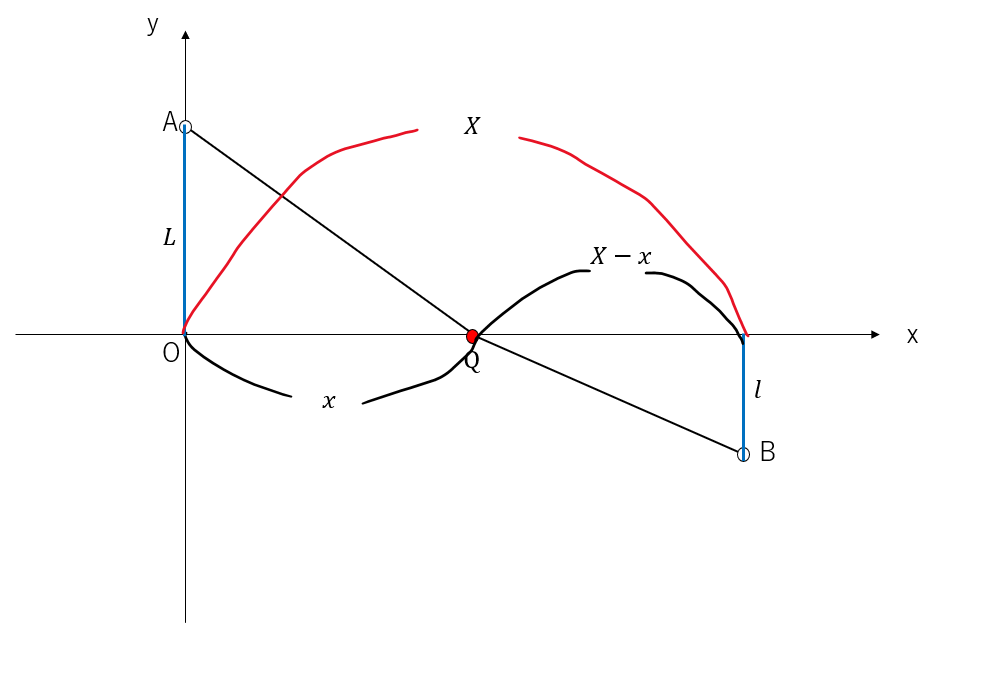
\includegraphics[scale=0.5]{img/QuuNote/Mondai2_12.png}
                        \end{figure}

                        この時、$A$から$B$まででかかる時間を$T(x)$とすると、
                        \begin{equation*}
                            T(x)=\frac{\sqrt{L^2+x^2}}{v_a}+\frac{\sqrt{l^2+(X-x)^2}}{v_b}
                        \end{equation*}
                        となる。よって、$x$微分すると
                        \begin{equation*}
                            \frac{dT}{dx} = \frac{x}{v_a \sqrt{L^2+x^2}}-\frac{X-x}{v_b\sqrt{l^2+(X-x)^2}}
                        \end{equation*}
                        しかし、このまま普通に$T'(x)=0$として$x$を求めようとしても、計算量が膨大で大変なことになる。よって少し賢いやり方をしよう。まず、$T'(0)<0,T'(X)>0$であるから、中間値の定理より
                        $T'(x)=0$をみたす$x$が区間$(0,X)$に少なくとも一つ存在することがわかる。さらに、第一項は単調増加、第二項は単調減少である。したがって、$T'(x)=0$のとき、式を移項すれば
                        $(\text{単調増加})=(\text{単調減少})$となり、解が一つしか存在しないことがわかる。よってその時の値を$x=x_0$とすれば、
                        先ほど述べたように$T'(0)<0,T'(X)>0$だから、$T(x_0)$が極小値であり、この区間で最小値だとわかる。すなわち$x=x_0$が求める解である。

                        とはいえ、何度も言うように$x_0$の値を具体的に求めることが難しい。しかし、我々が今求めたいのは$x_0$の値ではなく最短の経路である。今わかっている情報は$T'(x)=0$が成り立つ
                        とき、最短経路であるということである。これをもっと具体的な式で表してみよう。

                        まず、点$Q_0(x_0,0)$におけるx軸に垂直な直線を考え、この直線と線分$AQ_0$がなす角を$\theta_1$とする。同様に線分$BQ_0$となす角を$\theta_2$とする。
                        この時、$\displaystyle \sin\theta_1 = \frac{x}{\sqrt{L^2+x^2}},\sin\theta_2 = \frac{X-x}{\sqrt{l^2+(X-x)^2}}$である($\sin$の定義)。よって、$T'=0$は次のように書ける。
                        \begin{equation*}
                            T'=\frac{\sin \theta_1}{v_a}-\frac{\sin\theta_2}{v_b}=0
                        \end{equation*}
                        二項目を移項すれば
                        \begin{equation*}
                            \frac{\sin\theta_1}{v_a}=\frac{\sin\theta_2}{v_b}
                        \end{equation*}
                        つまり、この関係を満たす経路が求める経路である。これは光の屈折則(スネルの法則)に他ならない。

                    \paragraph{問13}$(1)y=\tan x$を方程式の左辺に代入し、$=0$になるか確かめよ。\hspace{1mm}$(2)$例えば$y=\tan(x+1).$一般に$y=\tan(x+a)$は解となる。

                    \paragraph{問14}ロピタルの定理を用いよ。
                        \begin{align*}
                            \lim_{x\to\infty}&\frac{x^n}{e^x} = 0\\
                            \lim_{x\to\infty}&\frac{\log x}{x^n} = 0 
                        \end{align*}
                        なお、この問題の結果は非常に重要なので覚えておこう。もっと言えば、$0<a<b$のとき、$n\to\infty$では
                        \begin{equation*}
                            \log n\ll {\small n^a} \ll {\normalsize n^b} \ll {\large e^{n}} \ll {\huge n!} 
                        \end{equation*}
                \clearpage
                \subsection*{第III部解答}
                    以下積分定数を$C$と置く。
                    \paragraph{問1}
                        $\displaystyle[1]\frac{x^7}{7}+\frac{3}{5}x^5+x^3+x+C\hspace{1mm}[2]x^2\sin x+2x\cos x-2\sin x+C\hspace{1mm}[3]\frac{1}{\sin x}=\frac{1}{2\sin\frac{x}{2}\cos\frac{x}{2}}=\frac{1}{2}\frac{1/\cos^2\frac{x}{2}}{\tan\frac{x}{2}}\text{だから}\log\left|\tan\frac{x}{2}\right|+C\hspace{1mm}[4]-\log|\cos x|+C
                        \hspace{1mm}[5]\cos x-\frac{2}{3}\cos^3x+\frac{1}{5}\cos^5x+C$\hspace{1mm}$[6]t^2=x-a$と置くと、$dx = 2tdt$であり、$x-\beta = t^2+\alpha -\beta$であるので、$\displaystyle \int \frac{2t}{\sqrt{t^2(t^2+\alpha-\beta)}}dt=2\int \frac{dt}{\sqrt{t^2+\alpha-\beta}}=2\log\left|t+\sqrt{t^2+\alpha-\beta}\right|=2\log\left|\sqrt{x-a}+\sqrt{x-\beta}\right|+C
                        \hspace{1mm}[7]\frac{x^2}{(x+1)^2(x-1)}=\frac{-1}{3(x+1)^2}+\frac{5}{9(x+1)}+\frac{4}{9(x-2)}\text{だから}\frac{1}{3}\frac{1}{x+1}+\frac{5}{9}\log|x+1|+\frac{4}{9}\log|x-2|+C\hspace{1mm}[8]\frac{1}{ab}\arctan\left(\frac{a}{b}\tan x\right)\hspace{1mm}\sqrt{1+\cos x}=\sqrt{2\cos^2\frac{x}{2}}=\sqrt{2}\cos^2\frac{x}{2}\text{より}2\sqrt{2}\sin\frac{x}{2}+C$
                    
                    \paragraph{問2}
                        $[1]12\sqrt{2}-8\hspace{1mm}[2]\pi\hspace{1mm}[3]\frac{2}{\pi}\hspace{1mm}[4]\frac{1}{x^2}\cdot(x-1)e^x\text{と分けて、$1/x^2$を積分する部分積分を実行。}\frac{e^2}{2}-e\hspace{1mm}[5]x=\tan\theta\text{と置くと}\frac{5}{6\sqrt{2}}\hspace{1mm}[6]\sin x-2\cos x = \sqrt{5}\sin(x-\sin^{-1}\frac{2}{\sqrt{5}})$であるから、区間$[0,\frac{\pi}{2}]$で
                        符号が変わるのは$x=\sin^{-1}\frac{2}{\sqrt{5}}$のとき。よって$[0,\frac{\pi}{2}]=[0,\sin^{-1}\frac{2}{\sqrt{5}}]+[\sin^{-1}\frac{2}{\sqrt{5}},\frac{\pi}{2}]$と区間を分けてそれぞれ計算すれば、$2\sqrt{5}-3$\hspace{1mm}$\displaystyle[7]I=\int_{0}^{\frac{\pi}{2}}\log\sin xdx \overset{x\to\frac{\pi}{2}-x}{=} \int_{0}^{\frac{\pi}{2}}\cos\log xdx=\frac{1}{2}\int_{0}^{\frac{2}{\pi}}\log(\sin x\cos x)dx = \frac{1}{2}\int_{0}^{\frac{\pi}{2}}\log(\frac{1}{2}\sin 2x)dx=\frac{1}{2}\int_{0}^{\frac{\pi}{2}}\log\sin2x-\log 2dx=\frac{\pi}{4}\log 2 + \frac{1}{2}\int_{0}^{\frac{\pi}{2}}\log\sin2xdx.$
                        ここで、最後の積分を$J$と置き、$2x\to x$の置換を行うと、$\displaystyle J=\frac{1}{4}\int_{0}^{\pi}\log\sin xdx =\frac{1}{4}I+ \frac{1}{4}\int_{\frac{2}{\pi}}^{\pi}\log\sin xdx\overset{x\to \pi-x}{=}\frac{1}{4}I+\frac{1}{4}\int_{0}^{\frac{\pi}{2}}\log\sin xdx = \frac{I}{2}.$したがって、$I=\frac{\pi}{4}\log 2 + J =\frac{\pi}{4}\log 2 + \frac{I}{2} \leftrightarrow I=-\frac{\pi}{2}\log 2\hspace{1mm}[8]\infty \hspace{1mm}[9]w>0\text{のとき収束して}\frac{1}{w}$\hspace{1mm}$\displaystyle[10]\frac{1}{ab}$\\
                        $[10]$はファインマンのパラメータ積分と呼ばれる。これにより、一般に$\frac{1}{a^nb^m}$を積分形で表せる。
                    
                    \paragraph{問3}
                        $\displaystyle(1)\int_{0}^{\pi}|\sin x-\cos x|dx = 2\sqrt{2}\hspace{1mm}(2)a>0$で考える。このとき、$y_+ = +\sqrt{r^2-x^2}+a,y_-=-\sqrt{r^2-x^2}+a$と置くと、求める体積は
                        $\displaystyle \pi\int_{-r}^{r}(y_+)^2-(y_-)^2dx = 2\pi a\cdot \pi r^2$となる。$a<0$のときも同様に考えて、$ 2\pi (-a)\cdot \pi r^2.$ここで、回転体の公式\eqref{eq:回転体の体積}を用いた。

                    \paragraph{問4}
                        $(1)g' = e^{-x}$として部分積分する。$\displaystyle\lim_{x\to\infty} \frac{x^s}{e^x}$は、$s>0$より$0$であることを利用せよ。\hspace{1mm}$(2)\gamma(1=1)$と$(1)$の結果を利用せよ。

                    \paragraph{問5}普通に部分積分すればよい。
                        \begin{equation*}
                            \int_{0}^{1}x^{m}(1-x)^ndx = \left[\frac{1}{m+1}x^{m+1}(1-x)^n\right]_0^1 + \int_{0}^{1}\frac{n}{m+1}x^{m+1}(1-x)^{n-1}dx = \frac{n}{m+1}\int_0^1 x^{m+1}(1-x)^{n-1}dx
                        \end{equation*}
                        あとはこれを、あとはこれを$n-1$回繰り返せば、
                        \begin{equation*}
                            \cdots = \frac{n!}{(m+1)(m+2)\cdots(m+n)}\int_{0}^{1}x^{m+n+1}dx = \frac{n!}{(m+1)\cdots (m+n+1)}=\frac{n!m!}{(m+n+1)!}
                        \end{equation*}
                        最後の式変形は分子分母に$m!$をかけた。
                    \clearpage
                    \paragraph{問6}
                        $n$が奇数のとき、被積分関数は機関数だから値は$0$である。(注:本来なら$\int_a^b,a\to\infty,b\to-\infty$なのだから、直ちにこの結果は得られない。しかし、$n=2k+1$と置いて、$t=x^2$の置換を行って実際に計算すると、
                        被積分関数は$t^{k}e^{-t}$の形になり、この$[a^2,b^2]$の積分は、部分積分を繰り返して結局0になる。)

                        よって、$n$が偶数のときを考える。$n=2k\quad(k=0,1,2,\dots)$とすると、
                        \begin{equation*}
                            G_{2k}=\int_{\infty}^{-\infty}x^{2k}e^{-x^2}dx = \left[-\frac{1}{2}e^{-x^2}x^{2k-1}\right]_{-\infty}^{\infty}+(2k-1)\int_{-\infty}^{\infty}x^{2(k-1)}e^{-x^2}dx
                        \end{equation*}
                        ここで、$g'=xe^{-x^2}$として部分積分を行った。さて、[\hspace{2mm}]内は結局0であるから
                        \begin{equation*}
                            G_{2k}=(2k-1)G_{2(k-1)}
                        \end{equation*}
                        よってこの漸化式を解けばよい。$G_0=\sqrt{\pi}$であるから、
                        \begin{equation*}
                            G_{2k} = (2k-1)G_{2(k-1)}=(2k-1)(2k-3)G_{2(k-2)}=\cdots =(2k-1)!!\sqrt{\pi} 
                        \end{equation*}
                        ここで二重階乗$!!$を用いた。例えば、$7!! = 7\times 5\times 3\times 1$である。(後ろのページの付録参照。)\\よってまとめると、$G_{2k}=(2k-1)!!\sqrt{\pi},I_{2k+1}=0.$

                    \paragraph{問7}
                        $t-\sqrt{a}x=\sqrt{ax^2+bx+c}\leftrightarrow t^2-2\sqrt{a}tx+ax^2 = ax^2+bx+c$
                        よって整理して、$\displaystyle x = \frac{1}{c}\left(\frac{t^2}{2\sqrt{a}t+b}\right)\leftrightarrow dx = \frac{1}{c}\left(\frac{2\sqrt{a}t^2+2bt}{(2\sqrt{a}t+b)^2}\right)dt$
                        また、$\displaystyle\sqrt{ax^2+bx+c} = t-\sqrt{a}x =t-\frac{\sqrt{a}}{c}\left(\frac{t^2}{2\sqrt{a}t+b}\right)$

                        したがって、元の積分は
                        \begin{equation*}
                            \int f(x,\sqrt{ax^2+bx+c})dx = \int f\left(\frac{1}{c}\left(\frac{t^2}{2\sqrt{a}t+b}\right),t-\frac{\sqrt{a}}{c}\left(\frac{t^2}{2\sqrt{a}t+b}\right)\right)\frac{1}{c}\left(\frac{2\sqrt{a}t^2+2bt}{(2\sqrt{a}t+b)^2}\right)dt
                        \end{equation*}
                        となり、$t$の有理関数で表せたので必ず積分できる。
                    
                    \paragraph{問8}
                        $(1)\sin(k\pi) =0$と$[\cos (n+1)\pi = \pm 1\leftrightarrow \cos n\pi = \mp 1]\Leftrightarrow \cos(n+1)\pi = (-1)^{n-1}$を利用する。$\int e^{-x}\sin xdx = \frac{-1}{2}e^{-x}\left\{\sin x+\cos x\right\}$より、
                        \begin{equation*}
                            I_n = -\frac{1}{2}\left[e^{-x}(\sin x+\cos x)\right]_{n\pi}^{(n+1)\pi}=\frac{(-1)^n}{2}\left(\frac{1}{e^{(n+1)\pi}}+\frac{1}{e^{n\pi}}\right)=\frac{(-1)^n}{2}(e^{-\pi}+1)e^{-n\pi}
                        \end{equation*}
                        $(2)$求める積分を$[0,\pi],[\pi,2\pi],\dots,[m,(m+1)\pi],\dots$に分割すれば、それぞれは$I_n$で与えられるので、これを足し合わせればよい。$m$回までの和は
                        \begin{equation*}
                            \sum_{n=0}^{m}\int_{n\pi}^{(n+1)\pi}e^{-x}|\sin x|dx = \sum_{n=0}^{m}\left|\frac{(-1)^n}{2}(e^{-\pi}+1)e^{-n\pi}\right| =\frac{e^{-\pi}+1}{2}\sum_{n=0}^{m}e^{-n\pi}=\frac{e^{-\pi}+1}{2}\left\{1+\sum_{n=1}^{m}e^{-n\pi}\right\}
                        \end{equation*}
                        ここで、求める和を$S_m$と置けば、
                        \begin{alignat*}{4}
                            S_m &= &e^{-\pi}+&e^{-2\pi}+&e^{-3\pi}+&\cdots + &e^{-m\pi}&{}\\
                            e^{-\pi}S_m &=&{}&e^{-2\pi}+&e^{-3\pi}+&\cdots + &e^{-m\pi}&+e^{-(m+1)\pi}
                        \end{alignat*}
                        であるから、$S_m-e^{-\pi}S_m = e^{-\pi}-e^{-(m+1)\pi}$である。すなわち、$\displaystyle S_m = \frac{e^{-\pi}(1-e^{-m\pi})}{1-e^{-\pi}}$

                        求める答えは、$m\to\infty$の極限であるから、この時$\displaystyle I=\frac{e^{-\pi}+1}{2}\cdot \left(1+\frac{e^{-\pi}}{1-e^{-\pi}}\right)=\frac{1}{2}\cdot \frac{1+e^{-\pi}}{1-e^{-\pi}.}$なお、
                        $S_m$を求める過程は、等比数列$a_n =ar^{n-1}$と置くと、一般に$\displaystyle S_n =\frac{a(1-r^{n})}{1-r}$で与えられる。 
                    \clearpage
                    \paragraph{問9}
                        \begin{equation*}
                            g(x)=\int_{0}^{x}f(t)\cos(x+t)dt=\int_{0}^{x}\left\{\cos x\cos t-\sin x\sin t\right\}dt=\cos x\int_{0}^{x}f(t)\cos tdt-\sin x\int_{0}^{x}f(t)\sin tdt
                        \end{equation*}
                        であるから、積の微分公式を用いて、\\
                        $\displaystyle g'(x)=\left(-\sin x\int_0^x f(t)\cos tdt+\cos^2xf(x)\right)-\left(\cos x\int_0^xf(t)\sin tdt+\sin^2 xf(x)\right)$すなわち、\\$g'(x)=\cos 2xf(x)-\int_0^xf(t)\sin(x+t)dt.$が答えになる。
                    
                    \paragraph{問10}$(1)$下図を参照。$S(\theta)=\frac{1}{2}r\sin\theta\cdot(r\sin\theta)\tan\frac{\pi}{4}=\frac{1}{2}r^2\sin^2\theta$
                        \begin{figure}[h]
                            \centering
                            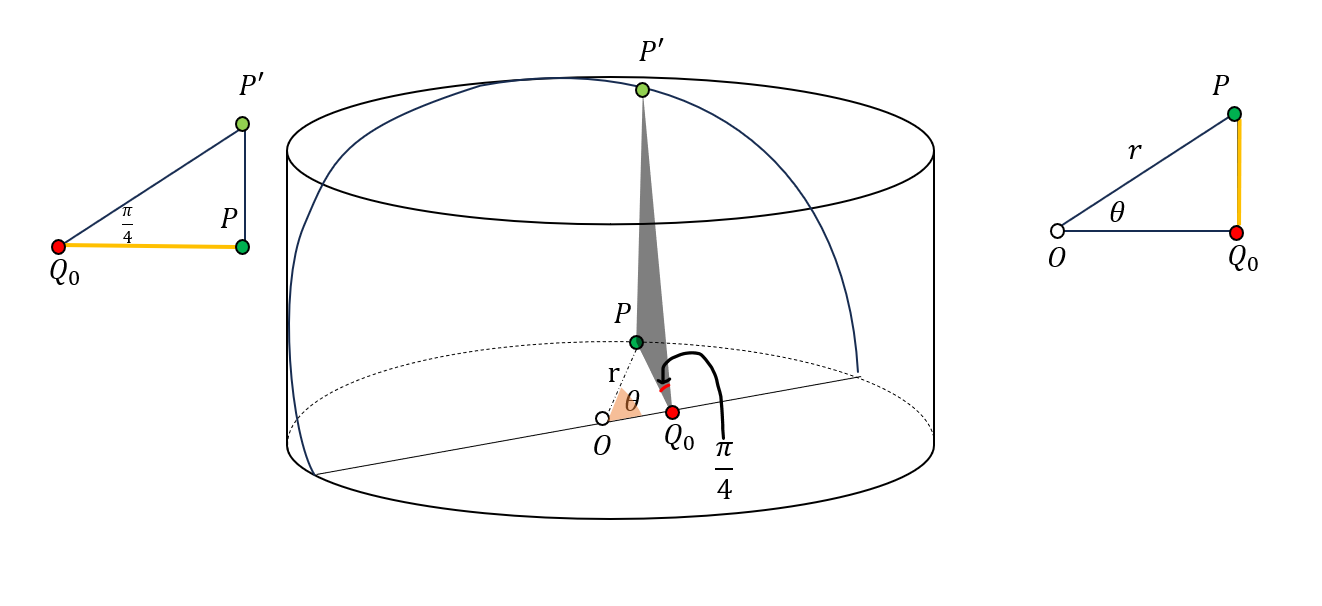
\includegraphics[scale=0.5]{img/QuuNote/Mondai3_10_1.png}
                        \end{figure}

                        $(2)\Delta \theta$が十分小さいとき、体積の微小変化$\Delta V$は以下図の三角柱のように近似できる。
                        \begin{figure}[h]
                            \centering
                            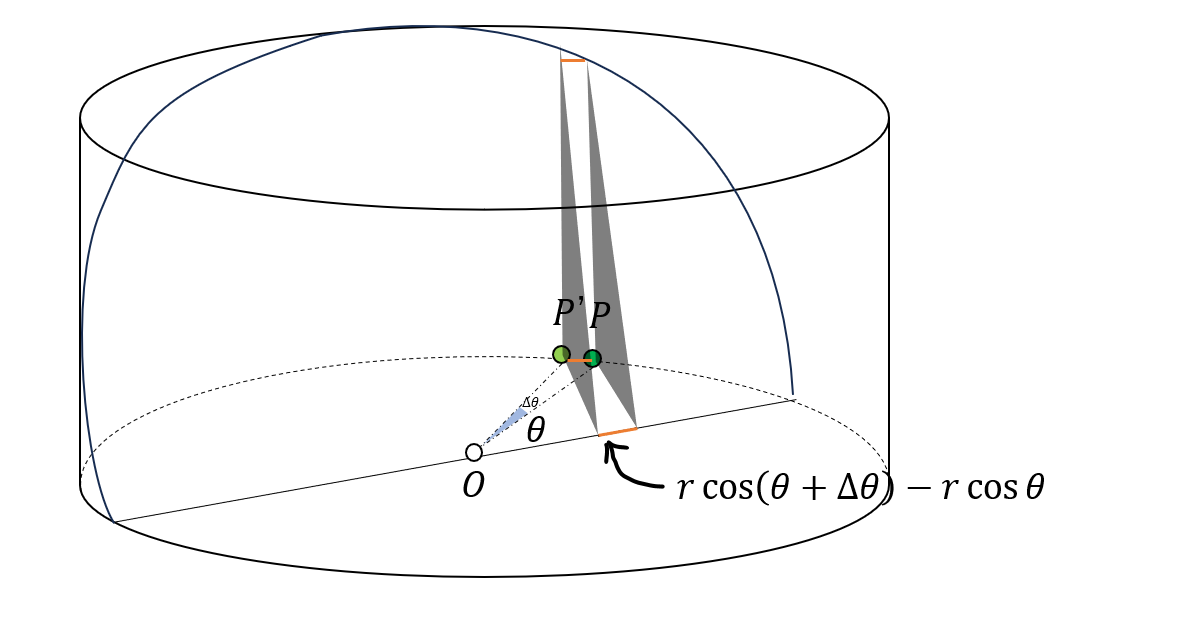
\includegraphics[scale=0.3]{img/QuuNote/Mondai3_10_2.png}
                        \end{figure}

                        \noindent したがって、$\Delta V=S(\theta)(r\cos(\theta+\Delta \theta)-r\cos\theta)=2rS(\theta)\sin\frac{\Delta \theta}{2}\sin\left(\theta+\frac{\Delta\theta}{2}\right).$\\

                        $(3)$求める体積$V$は、区間$\theta\in[0,\pi]$を$n$分割し、各区間の任意の角度を$\theta_k$、各``幅''を$\Delta \theta_k$と置くと、次のように近似できる。
                        \begin{equation*}
                            S_\Delta =\sum_{k=1}^{n}rS(\theta_k)\sin\frac{\Delta\theta_k}{2}\sin\left(\theta_k+\frac{\Delta\theta_k}{2}\right)=2r^3\sum_{k=1}^{n}\sin^2\theta_k \sin\left(\theta_k+\frac{\Delta \theta_k}{2}\right)\cdot \frac{\sin\frac{\Delta \theta_k}{2}}{\frac{\Delta\theta_k}{2}}\Delta \theta_k
                        \end{equation*}
                        ここで、分割数$n$を限りなく大きくすると、$\Delta \theta_k\to 0$だから、$\displaystyle \sin\left(\theta_k +\frac{\Delta\theta_k}{2}\right)\to\sin\theta_k,\frac{\sin\frac{\Delta \theta_k}{2}}{\frac{\Delta\theta_k}{2}}\to 1$であるから、この極限は積分を用いて次のように表せる。
                        \begin{equation*}
                            V=\frac{r^3}{2}\int_{0}^{\pi}\sin^3\theta d\theta
                        \end{equation*}
                        よって、求める体積は$V=\frac{2}{3}r^3.$

                        実は、このやり方を行わなくても、$S(\theta)$を$x$の関数で表せば、これの$[-r,r]$の積分で答えが求められる。このように、図形の体積を求める問題は、
                        断面積の求め方が``かんどころ''になってくる。このやり方のように計算量の少ないやり方もあれば、問題のやり方のように計算量がとんでもないし、近似計算
                        ばかりで厳密な答えなのか疑ってしまうようなやり方もある。それでもこの複雑なやり方を問題に選んだのは、式中に$\sqrt{}$が出てくるのをむやみに嫌がって別の
                        やり方を試そうとする人への警告である。
                \clearpage
                \subsection*{第IV部解答}
                    \paragraph{問1}[1]発散[2]発散[3]収束[4]発散[5]収束[6]$\displaystyle f(x)=\frac{\log x}{x}$と置くと、$f$は$x>e>2$で単調減少だから$\int_3^\infty f(x)dx $
                    が収束するかを調べればよい。この積分は発散するので、発散.

                    \paragraph{問2}
                    絶対収束するとき収束するので、以降わざわざ収束まで書かない。
                    [1]条件収束[2]絶対収束[3]条件収束[4]発散[5]絶対収束.\hspace{2mm}ここで[4]は「$\lim a_n\neq 0\rightarrow\sum a_n$発散」を用いた。
                
                    \paragraph{問3}
                        $[1]-1\leq x\leq 1\hspace{1mm}[2]-3\leq x<3\hspace{1mm}[3]-\infty <x<\infty\hspace{1mm}[4]x\leq 0\hspace{1mm}[5]$
                        $\displaystyle \frac{1}{(x+n-1)(x+n)}=\frac{1}{x+n-1}-\frac{1}{x+n},S_n = \left(\frac{1}{x}-\frac{1}{x+1}\right)+\left(\frac{1}{x+1}-\frac{1}{x+2}\right)+\cdots+\left(\frac{1}{x+n-1}-\frac{1}{x+n}\right)=\frac{1}{x}-\frac{1}{x+n}$
                        したがって、$x\neq 0$で$\displaystyle \lim_{n\to\infty}S_n = \frac{1}{x}.$さらに、$n=1,2,3,\cdots$だから、$n\to\infty$で$x+n \neq 0$であるためには$x\neq -1,-2,-3,\dots$であればよい。したがって、$x\neq  0,1,2,3,\dots$で収束.

                    \paragraph{問4}$(1)\displaystyle f(x)=\frac{1}{x+1}$と置くと、$f^{(n)}(x)=\frac{(-1)^nn!}{(x+1)^{n+1}}$であるので、$f^{(n)}(0)=(-1)^nn!.$よって、$\displaystyle \frac{1}{x+1}=\sum_{n=0}^\infty(-1)^n n!\cdot \frac{x^n}{n!}=\sum (-1)^nx^n.$$x$の収束する範囲は$-1< x< 1.$
                    \hspace{1mm}$(2)f(x)$に$x=x^2$を代入せよ。$\displaystyle \frac{1}{1+x^2}=\sum_{n=0}^\infty (-1)^n x^{2n}.$$x$の収束する範囲は$-1<x<1.$
                    \hspace{1mm}$(3)\int f(x^2)dx =\arctan x$を利用する。$(2)$の式を積分すると、$\displaystyle \arctan x = \int_{0}^{x}\frac{dx}{1+x^2}=\sum_{n=0}^{\infty}\frac{(-1)^n}{2n+1}x^{2n+1}.$
                    $x$の収束する範囲は$-1\leq x\leq 1.$

                    \paragraph{問5}$(1)\displaystyle \frac{1}{n^2(n+1)^2}=\frac{1}{n^2}+\frac{1}{(n+1)^2}-2\left(\frac{1}{n}-\frac{1}{n+1}\right)$\hspace{2mm}
                    $(2)$求める級数の第$n$部分和$S_n$は、$(1)$より$\displaystyle \frac{1}{n}-\frac{1}{n+1}$の項は相殺されて$1-\frac{1}{n+1}$となり、$\displaystyle \frac{1}{n^2}+\frac{1}{(n+1)^2}$の項は、
                    $\displaystyle \sum_{m=1}^{n}\frac{1}{(m+1)^2}=\sum_{m=1}^{n}\frac{1}{m^2}-1+\frac{1}{(n+1)^2}$であるから、
                    \begin{equation*}
                        S_n = 2\sum_{m=1}^{n}\frac{1}{m^2}-1+\frac{1}{(n+1)^2}-2\left(1-\frac{1}{n+1}\right)
                    \end{equation*}
                    ここで$n\to \infty$の極限を取ると、求める級数の和は、$\frac{\pi^2}{3}-2$だとわかる。

                    \paragraph{問6}
                        $\displaystyle f(x)=\frac{1}{\sqrt{1-x}}$と置くと、$f^{(n)}(x)=\frac{(2n-1)!!}{2^n}(1-x)^{-\frac{1}{2}-n}$であるから、$\displaystyle f^{(n)}(0)=\frac{(2n-1)!!}{2^n}$である。
                        したがって、$f(x)$のマクローリン級数は、$\displaystyle f(x)=\sum_{n=0}^{\infty}\frac{(2n-1)!!}{2^nn!}x^n$である。また、収束半径は$r=1$である。
                        ここで、$2^nn!=(2\times 1) \times (2\times 2)\times \cdots\times  (2\times n)=(2n)!!$であるから、$\displaystyle \frac{1}{\sqrt{1-x}}=\sum \frac{(2n-1)!!}{(2n)!!}x^n$とできる。
                        $k^2<1$で、もちろん$\sin^2\phi \leq 1$だから、$0<k^2\sin^2\phi<1$よって、$f(k^2\sin^2\phi)$としてもよい。このとき楕円積分は、
                        \begin{equation*}
                            K(k)=\sum_{n=0}^{\infty}\frac{(2n-1)!!}{(2n)!!}k^{2n}\cdot \int_{0}^{\pi}\sin^{2n}\phi d\phi
                        \end{equation*}
                        である。ここで、積分区間を$[0,\frac{\pi}{2}],[\frac{\pi}{2}\pi]$に分け、後者の積分に$\phi \to \pi -\phi$の置換を行うと、$\displaystyle \int_{0}^{\pi}\sin^{2k}\phi d\phi = 2\int_{0}^{\frac{\pi}{2}}\sin^{2k}\phi d\phi $
                        とできる。よって、$\displaystyle I_m=\int_{0}^{\frac{\pi}{2}}\sin^{m}\phi d\phi$の積分を考察していく。
                        \clearpage
                        $\sin^{m}\phi = \sin\phi\cdot \sin^{m-1}\phi$と変形し、部分積分を行うと、\\
                        $\displaystyle I_m = \left[-\cos\phi\sin^{m-1}\phi\right]_0^{\frac{\pi}{2}}+\int_{0}^{\frac{\pi}{2}}\cos\phi\cdot (m-1)\sin^{m-2}\phi\cdot \cos\phi d\phi=(m-1)\int_{0}^{\frac{\pi}{2}}\sin^{m-2}\phi-\sin^{m}\phi d\phi = (m-1)(I_{m-2}-I_m)$となる。
                        ここで、$\cos^2 \phi =1-\sin^2\phi$を用いた。よって、式を整理して、$\displaystyle I_m=\frac{m-1}{m}I_{m-2}$の漸化式を解けばよい。すぐわかるように、$I_0 = \frac{\pi}{2}$であるから、
                        $m=2k$のとき、
                        \begin{equation*}
                            I_{2k} = \frac{2n-1}{2n}I_{2n-2}=\frac{2n-1}{2n}\frac{2n-3}{2n-2}I_{2n-4}=\cdots=\frac{(2n-1)!!}{(2n)!!}I_0=\frac{(2n-1)!!}{(2n)!!}\frac{\pi}{2}
                        \end{equation*}
                        この結果を$K(k)$の式に代入すれば、
                        \begin{equation*}
                            K(k)=\sum_{n=0}^{\infty}\frac{(2n-1)!!}{(2n)!!}k^{2n}\cdot \left\{\frac{(2n-1)!!}{(2n)!!}\frac{\pi}{2}\right\}=\frac{\pi}{2}\sum_{n=0}^{\infty}\left\{\frac{(2n-1)!!}{(2n)!!}\right\}k^{2n}
                        \end{equation*}
                        したがって、
                        \begin{equation*}
                            T=4\sqrt{\frac{l}{g}}K(k)=2\pi \sum_{n=0}^{\infty}\left\{\frac{(2n-1)!!}{(2n)!!}\right\}^2k^{2n}
                        \end{equation*}
                        が示された。\\

                        なお、途中に出てきた積分$\int_{0}^{\frac{\pi}{2}}\sin^{n}xdx$をウォリス積分という。$n=2m+1$のときは、
                        \begin{equation*}
                            \int_{0}^{\frac{\pi}{2}}\sin^n x dx=\frac{(2m)!!}{(2m+1)!!}
                        \end{equation*}
                        である。ここで$I_1=1$を利用した。
                                            
        \clearpage
            
        \color{black}
        \section{付録}
            \subsection{人名}
                数学を学ぶ上で様々な人の名前を冠した定理や公式が登場する。このノートではカタカナで書いてきたが、実際にほかの書籍を読む際などは英名で書かれる場合が多い。そこで
                以下に対応の表を載せる。「主な定理等」にはその人が発見・発明した解析学関係のことを述べる。
                
                \begin{table}[h]\hspace{-2.5cm}
                    \begin{tabular}{|c|c|c|l|}\hline
                        名前 & 名前(英)& 主な定理等 & メモ\\\hline\hline
                        オイラー & Euler & オイラーの公式など & \begin{tabular}{l}18世紀最大の数学者であり、その業績は解析学に留まらない。\\オイラーの名を冠する定理も多い。\end{tabular}\\\hline
                        ニュートン & Newton & 流率法 & \begin{tabular}{l}古典力学の創始者。\\リンゴの落下から万有引力を思いついた逸話は非常に有名。\end{tabular}\\\hline
                        ライプニッツ & Leibniz & 微積分法の発明 & \begin{tabular}{l}ニュートンとは独立に微積分を発明させた。\\また、記号$\int\frac{d}{dx}$などはライプニッツによるものである。\end{tabular} \\\hline
                        コーシー & Cauchy & コーシーの積分定理 & \begin{tabular}{l}収束について厳密な定義を考え、のちの$\varepsilon-\delta$論法の原型となった。\\複素解析の業績がとくに有名。\end{tabular} \\\hline
                        ラグランジュ &  Lagrange & - & \begin{tabular}{l}解析力学を構築し、ニュートン力学を発展させた。\\ラグランジュの未定乗数法などでもその名前を見かける。\end{tabular}\\\hline
                        リーマン & Riemann & リーマン幾何学/リーマン積分 & \begin{tabular}{l}複素解析のパイオニア。彼が予想したリーマン予想は数学の重要な\\未解決問題の一つであり、ミレニアム懸賞問題のうちの一つである。\end{tabular}\\\hline
                        ガウス & Gauss & - & \begin{tabular}{l}オイラーと双璧をなす19世紀最大の数学者。数論の分野での功績\\が大きい。彼の名前の付いた法則・記号・単位も多い。\end{tabular}\\\hline
                        ウォリス & Wallis & ウォリス積分/ウォリスの公式 & \hspace{2mm}無限大の記号$\infty$を導入した。\\\hline
                        テイラー & Taylor & テイラーの定理/テイラー展開 & \hspace{2mm}特になし\\\hline
                        マクローリン & Maclaurin & マクローリン展開 & \hspace{2mm}特になし\\\hline
                        ベルヌーイ & Bernoulli & - & \begin{tabular}{l}ヨーロッパの数学者一族の総称。ベルヌーイ数、ベルヌーイの定理\\などベルヌーイの名前が付いたものも多い。\end{tabular}\\\hline
                        ロピタル & l'Hôpital & - & \begin{tabular}{l}初めて微分積分の書籍を出したことで有名。\\ちなみにロピタルの定理はロピタル自身が発見したのではなく\\ヨハン・ベルヌーイによるものである。\end{tabular}\\\hline
                        フーリエ & Fourier & フーリエ級数/フーリエ変換 & \begin{tabular}{l}関数を三角関数の級数で表すというアイデアから始まったフーリエ\\解析は、解析学の厳密化に貢献しただけでなく、物理や工学の幅広い\\部分で応用されている。また、ナポレオンのエジプト遠征に同行した\\ことでも有名。\end{tabular}\\\hline
                        デデキント &  Dedekind & - & \begin{tabular}{l}デデキントカット(切断)という方法で実数を定義。これは解析概論\\でも用いられている手法である。\end{tabular}\\\hline
                        {\footnotesize ワイエルシュトラス} & Weierstrass & - & \hspace{2mm}ワイエルシュトラスの$W$関数なども有名。\\\hline
                        ルベーク & Lebesgue & ルベーク積分 & ここら辺の話は集合論とも絡み合って非常に難しい。\\\hline
                    \end{tabular}                    
                \end{table}
            \clearpage
            \subsection{文字・記号とその名称}
                微積分に限らず数学ではよくギリシャ文字や様々な演算子を用いたりする。しかしそれらの文字をどう読むのかまで書いてあるものは少ない。そこで以下に対応表のつけた。
                \begin{table}[h]
                    \caption*{ギリシャ文字}
                    \centering
                    \begin{tabular}{|c|c|l||c|c|l|}\hline
                        大文字 & 小文字 & \multicolumn{1}{c||}{読み方} & 大文字 & 小文字 & \multicolumn{1}{c|}{読み方} \\\hline\hline
                        A & $\alpha$ & アルファ & N & $\nu$ & ニュー\\\hline
                        B & $\beta$ & ベータ & $\Xi$ & $\xi$ & クシー(クサイ)\\\hline
                        $\Gamma$ & $\gamma$ & ガンマ & O & $o$ & オミクロン \\\hline
                        $\Delta$ & $\delta$ & デルタ & $\Pi$ & $\pi$ & パイ\\\hline
                        E & $\varepsilon$ & イプシロン & P & $\rho$ & ロー \\\hline
                        Z & $\zeta$ & ゼータ & $\Sigma$ & $\sigma,\varsigma$ & シグマ\\\hline
                        H & $\eta$ & イータ & T & $\tau$ & タウ\\\hline
                        $\Theta$ & $\theta,\vartheta$ & シータ & $\Upsilon$ & $\upsilon$ & ウプシロン\\\hline
                        I & $\iota$ & イオタ & $\Phi$ & $\phi,\varphi$ & ファイ\\\hline
                        K & $\kappa$ & カッパ & X & $\chi$ & カイ\\\hline
                        $\Lambda$ & $\lambda$ & ラムダ & $\Psi$ & $\psi$ & プサイ\\\hline
                        M & $\mu$ & ミュー & $\Omega$ & $\omega$ & オメガ \\\hline
                    \end{tabular}
                    
                    \caption*{数学の記号}
                    \centering
                    \begin{tabular}{|c|c|l|}\hline
                        記号 & 読み方 & \multicolumn{1}{c|}{意味}\\\hline
                        $\forall$ & 任意の-/すべての- & 全称記号。$\forall x \in \mathbb{N}$は「任意の自然数$x$について-」の意。\\\hline
                        $\exists$ & ある-/-が存在して & 存在記号。$\exists x \in \mathbb{N}$は「ある自然数$x$に対して-」の意。 \\\hline
                        $!$ & 階乗 & ある正の整数から$1$までの整数の積\\\hline
                        $!!$ & 二重階乗(二度びっくり?) & 階乗の一個飛ばし版。ex:\hspace{1mm}$5!!=5\times3\times1/(0)!!=(-1)!!=0$\\\hline
                        $\int$ & インテグラル & 積分 \\\hline
                        $\partial$ & ラウンドディー/デル/パーシャル & 偏微分で用いられる。\\\hline
                        $f^{-1}(x)$ & エフ・インバース・エックス & $f(x)$の逆関数\\\hline
                        $\lim$ & リミット & 極限の操作。通常$\displaystyle\lim_{x\to a}$のように用いる。\\\hline
                        $\nabla$ & ナブラ & 微分作用素の一つ。$\nabla=\left(\frac{\partial}{\partial x},\frac{\partial}{\partial y}\right)$\\\hline
                        $\mathrm{div}$ & ダイバージェンス & ベクトル場に用いる演算子。ベクトル場の発散(divergence)を表す。\\\hline
                        $\mathrm{rot}$ & ローテーション & ベクトル場に用いる演算子。ベクトル場の回転(rotation)を表す。\\\hline
                        $\mathrm{grad}$ & グラディエント & スカラー場に用いる演算子。スカラー場の勾配(gradient)を表す。\\\hline
                        $\varDelta$ & ラプラス作用素/ラプラシアン & 微分作用素の一つ。ナブラ同士の内積として与えられる。\\\hline
                    \end{tabular}
                \end{table}
        \clearpage
        \subsection{ベクトル解析入門}
            本来ならここで終わる予定であったが、シラバスを確認したところ3Eでは専門科目でベクトル解析を扱うようであるのでここで少しだけ勉強しよう。\footnote{25/01/12校正時追加 シラバスではベクトル解析をフルで使う書き方をしていたが、実際はほとんど使わなかった。むしろ飛ばした面積分を使ったのは皮肉か。}\\

            まず、ベクトルについて。こちらは直感的に分かりやすい定義を採用して、``向きと大きさ''を持つ量としよう。スカラーは``大きさ''だけを持つ量とする。
            以降は太字で書いたものをベクトルとする。例えば、$\bm{a}$はベクトルで$a$はスカラーを表す。また、ベクトルの大きさ(長さ)を$|\bm{a}|$や$\|\bm{a}\|$と表す。

            ベクトルには2種類の積が定義できる。一つ目は、スカラー積、いわゆる\textbf{内積}。もう一つはベクトル積、別の言い方をすれば\textbf{外積}である。
            内積は、二つのベクトル$\bm{a},\bm{b}$のなす角度を$\theta$とすれば、$\bm{a}\cdot\bm{b}=\|\bm{a}\|\|\bm{b}\|\cos\theta$であり、外積は、$\bm{i}=[1,0,0],\bm{j}=[0,1,0],\bm{k}=[0,0,1]$
            とすれば、
            \begin{equation}
                \bm{a}\times \bm{b} = 
                \begin{vmatrix}
                    \bm{i} & \bm{j} & \bm{k} \\
                    a_1 & a_2 & a_3 \\
                    b_1 & b_2 & b_3
                    \end{vmatrix}                    
            \end{equation}
            で表せる。これは行列式の中にベクトルが入っているのであくまで形式的な表現であることに注意されたい。外積の演算結果はベクトルである。また、外積の定義からわかるように外積では交換則が成り立たない。
            外積は、二つのベクトル$\bm{a},\bm{b}$に直行するベクトルを与える。三次元だと二つ存在するが、例えばベクトル
            $\bm{a}\times \bm{b}$は、ベクトル$\bm{a}$から$\bm{b}$の方向に右ネジを回すときのネジの進む方向となる。

            次に\textbf{ベクトル値関数}を定義する。これは独立変数(スカラー)を$t$に対して、従属変数は各成分が$t$の関数となるベクトルのことである。これを$\bm{a}(t)$のように書く。
            ベクトルの関数といわれて少し戸惑ってしまうが、少しも怖がる必要はない。ベクトルも所詮スカラーをまとめて扱っているだけなので、結局各成分が$t$の関数となるだけなのである。式で書けば、
            $\bm{a}(t)=[a_1(t),a_2(t),a_3(t)]$である。

            さて、ベクトル値関数といえども関数の仲間であるので、当然微分を定義したくなるのが人間の性であろう。実際定義出来て、
            \begin{equation}
                \frac{d}{dt}\bm{a}(t)=\lim_{t\to 0}\frac{\bm{a}(t+h)-\bm{a}(t)}{h}=[a_1'(t),a_2'(t),a_3'(t)]
            \end{equation}
            である。結局成分を微分するだけである。なお、これは極限や積分についても同じである。

            本来ならここでフレネ・セレの公式やそれに関連する話題などなどを紹介したいが、どうやら3Eでは使わなそうなので今回は割愛する。ここの話もすごく面白いところなので興味を持った人がいたらぜひ勉強してほしい。

            話はいったん多変数の微分積分に移る。まず、二変数関数$z=f(x,y)$について、\textbf{偏微分}を定義する。
            \begin{equation}
                \frac{\partial f}{\partial x}=\lim_{\delta x\to 0}\frac{f(x+\Delta x,y)-f(x,y)}{\Delta x}
            \end{equation}
            を$f(x,y)$の$x$に関する偏導関数といい、$f_x$と略記することもある。もちろん$y$についても定義できる。これらの偏導関数を求めることを偏微分するという。これは多変数関数でも同様に定義される。

            ベクトル解析に話を戻す。まず、空間上の領域$D$の各点に、ベクトル$\bm{f}(x,y,z)$が対応づけられているとき、この領域$D$のことを
            (空間)\textbf{ベクトル場}という。同様にスカラー場も定義される。ベクトル場は領域のことを指すが、ベクトル値関数$\bm{f}$と同一視してよい。

            ここで、\textbf{勾配ベクトル}(gradient)を次のように定義する。
            \begin{equation}
                \mathrm{grad} f = \left[\frac{\partial f}{\partial x},\frac{\partial f}{\partial y},\frac{\partial f}{\partial y}\right]
            \end{equation}
            ここで、$f(x,y,z)$はスカラー場である。勾配ベクトルの物理的意味は、平面スカラー場$f(x,y)$で考えるとわかりやすい。スカラー場の各点$(x,y)$で傾斜が最も
            な方向が勾配ベクトルの方向になる。

            いま、\textbf{ナブラ}(ハミルトン演算子)を定義する。
            \begin{equation}
                \nabla =  \left[\frac{\partial }{\partial x},\frac{\partial }{\partial y},\frac{\partial }{\partial y}\right]
            \end{equation}
            この演算子をスカラー場に作用、すなわち$\nabla f$は、勾配ベクトルと等しいことがすぐわかる。このナブラ記号を使えばベクトル解析の演算子を統一的に表すことできる。

            次に、ベクトル場の\textbf{発散}(divergence)を次のように定義する。$\bm{f}=[f_1,f_2,f_3]$とする。
            \begin{equation}
                \mathrm{div} \bm{f} = \frac{\partial f_1}{\partial x}+\frac{\partial f_2}{\partial y}+\frac{\partial f_3}{\partial z}
            \end{equation}
            定義からわかるように、発散はスカラーである。また、発散はナブラ記号を使えば、$\nabla\cdot \bm{f}$と表すことができる。発散の意味は、名前からも想像できるように、
            ベクトル場のわきだし量を表す。よくたとえで挙がるのが水量である。例えば、すべて同じ方向を向いている水が流れる川に関所を配置した時を考えてみよう。この時、
            関所に入ってくる水と関所から出ていく水の差、すなわち正味の水の流入(出)量が発散に当たる。雨が降ったり、川にホースで水が入れられたりしたら、その地点での水の量は変化する。
            これを数式で表してみる。水の量を$w$,水の位置を$x$と置くと、水の変化量は$\frac{dw}{dx}$で表すことができる。$\frac{dw}{dx}=0$なら、正味の水量の変化は$0$、つまり雨も降っていないし
            ホースで水が足されたりなんかもしていない。しかし、何らかの原因で水が足されると、$\frac{dw}{dx}>0$となる。水量の変化が正、つまり水が足されたというわけである。$\frac{dw}{dx}<0$の場合も同様に考えられる。

            以上をまとめると、$\frac{dw}{dx}$が川の正味の水量変化を表していることになる。今は一次元(川の水の流れが一方向)で考えたが、
            これを二次元、三次元で考えると当然$w$は多変数関数になるので、偏微分が使われる。発散の定義からわかるように、水量の正味の変化は各方向x,y,zの正味の変化を足し合わせたものである。

            最後に、ベクトル場の\textbf{回転}(rotation)を次のように定義する。
            \begin{equation}
                \mathrm{rot}\bm{f}=\left[\frac{\partial f_3}{\partial y}-\frac{\partial f_2}{\partial z},\frac{\partial f_1}{\partial z}-\frac{\partial f_3}{\partial x},\frac{\partial f_2}{\partial x}-\frac{\partial f_1}{\partial y}\right]
            \end{equation}
            複雑そうな式だなぁ...。と少し式のインパクトに気圧されそうになるが、安心してほしい。これもナブラ記号を用いて書けば$\nabla \times \bm{f}$で終わりである。
            ナブラ記号のなんと簡潔なことか。定義を見ればすぐわかるように、回転はベクトルである。これは何を意味しているのだろうか。
            実はこのベクトルの方向を右ネジの進む向きとしたときの、ネジの回る方向がベクトル場$\bm{f}$の回転方向を表している。なぜそうなるかの説明は面倒なのでここではしない。\\

            以上がベクトル解析入門の内容である。本来ならストークスの定理やガウスの発散定理も入れればよかったが、おそらく使わないだろうから泣く泣く飛ばした。そもそも
            限られたページ数ですべてを説明することなど不可能に近いのだから仕方ない。これにより3Eの電磁気学を乗り越えれることを祈るばかりだ。\footnote{25/01/12校正時追加 実際講義を受けた感想としては、ただの``お遊び''のようなものだと感じた。
            心配は杞憂に終わってよかったが、物足りない感じもある。}
        
        \clearpage
            \subsection*{メモ欄}
        \clearpage
            \subsection*{メモ欄}
        \clearpage

        \thispagestyle{fancy}
        \fancyhead{}
        \fancyfoot{\centerline{\hyperref[目次]{目次に戻る}}}

        \vspace{\stretch{1}}
        \begin{figure}
            \centering
            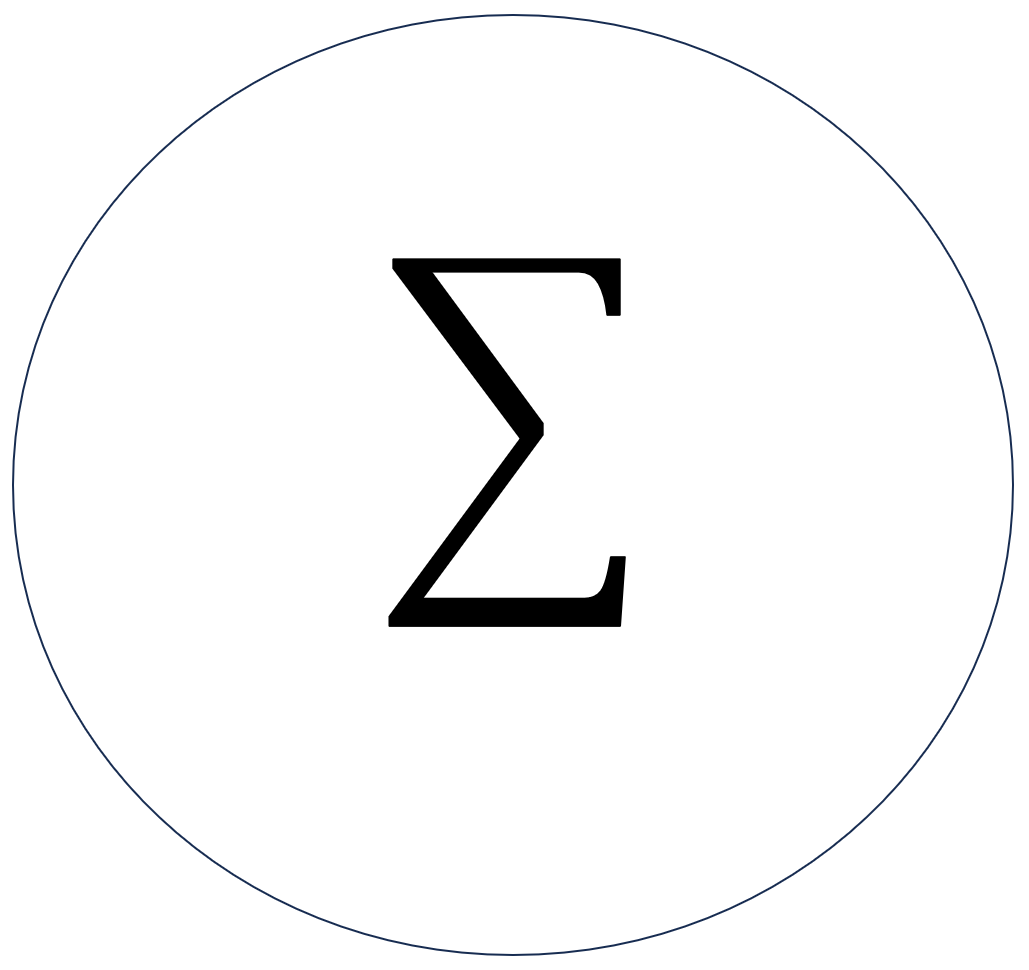
\includegraphics[scale=0.5]{img/QuuNote/icon.png}
        \end{figure}    
        \vspace{\stretch{1}}

        

\end{document}